%%%%%%%%%%%%%%%%%%%%%%%%%%%%%%%%%%%%%%%%%%%%%%%%%%%%%%%%%%%%%%%
\documentclass[12pt]{book}
\usepackage[a4paper,top=1.5in,bottom=1.5in,left=1in,right=1in]{geometry} 
\usepackage{fancyhdr}
\usepackage{fourier-orns}
\pagestyle{fancy}
\usepackage{graphicx}
\usepackage{lipsum} % for dummy text, you can remove this line in your actual document

\usepackage{amsmath, amssymb, bm}
\usepackage{caption}
\usepackage{graphicx} 
\usepackage[colorinlistoftodos]{todonotes}
\usepackage[colorlinks=true, allcolors=teal]{hyperref}
\usepackage{float}
\usepackage{setspace}
% \usepackage{subfigure}
\usepackage{url}
\usepackage{tabularx}
\usepackage[utf8]{inputenc}
\usepackage{mathptmx} %Times Font
\usepackage{titlesec}
\titlespacing{\chapter}{0pt}{0pt}{0pt}
\usepackage{fancyhdr}
\usepackage{etoolbox}
% \usepackage{appendix}
\usepackage{siunitx}
\usepackage{nomencl}
\newcommand{\nomunit}[1]{%
\renewcommand{\nomentryend}{\hspace*{\fill}#1}}
\makenomenclature%
\usepackage{caption}
\usepackage{lipsum}
\usepackage{algpseudocode}
\usepackage{empheq}
\usepackage{mdwlist}
\usepackage{booktabs}
\usepackage{colortbl}
\widowpenalty10000
\clubpenalty10000
\usepackage{moresize}
\usepackage{tabularray}
\usepackage[style=apa, backend=biber]{biblatex}
\usepackage{subcaption}
\usepackage{array}
\usepackage{adjustbox}
% \usepackage{algorithmic}
\usepackage{amsmath}
\usepackage{amsthm}
\usepackage{algorithm}
\usepackage[toc,page]{appendix}

\addbibresource{References.bib}
\DeclareSourcemap{
  \maps[datatype=bibtex]{
    \map{
       \step[fieldsource=title, match=\regexp{\b([A-Z]{2,})\b}, replace={{}{$1}}]
    }
  }
}
 
\DeclareCaptionType{appfigure}[Figure]
\DeclareCaptionType{apptable}[Table]
\renewcommand{\listappfigurename}{List of Appendix Figures}
\renewcommand{\listapptablename}{List of Appendix Tables}
\renewcommand{\thefigure}{\thechapter-\arabic{figure}}
\renewcommand{\thetable}{\thechapter-\arabic{table}}
\renewcommand{\theappfigure}{\thechapter-\arabic{appfigure}}
\renewcommand{\theapptable}{\thechapter-\arabic{apptable}}
\renewcommand{\contentsname}{Table of Contents}
\renewcommand{\thefigure}{\arabic{figure}}
\renewcommand{\thetable}{\arabic{table}}

\newcommand{\chapname}{Chapter }
 
\titleformat{\chapter}[block]
{\bfseries\LARGE\centering}
{}{1em}{}[\rule{\textwidth}{0.3pt}]

\titleformat{\section}
{\bfseries\large}
{\thesection}{1em}{}

\titleformat{\subsection}
{\normalfont\bfseries}
{\thesubsection}{1em}{}

\titleformat{\subsubsection}
{\normalfont\bfseries}
{\thesubsubsection}{1em}{}

\usepackage{fancyhdr}
\usepackage{multirow}
\usepackage{multicol}

\usepackage{placeins}

\makeatletter
\renewcommand*\env@matrix[1][*\c@MaxMatrixColsc]{%
  \hskip -\arraycolsep%
  \let\@ifnextchar\new@ifnextchar%
  \array{#1}}
\makeatother

\usepackage{enumitem}

\usepackage{listings}
\usepackage{color}
 
\definecolor{codegreen}{rgb}{0,0.6,0}
\definecolor{codegray}{rgb}{0.5,0.5,0.5}
\definecolor{codepurple}{rgb}{0.58,0,0.82}
\definecolor{backcolour}{rgb}{0.95,0.95,0.95}

\newcommand{\codesize}{\fontsize{10pt}{11pt}\selectfont}

\lstdefinestyle{mystyle}{
    backgroundcolor=\color{backcolour},   
    commentstyle=\color{codegreen},
    keywordstyle=\color{magenta},
    numberstyle=\tiny\color{codegray},
    stringstyle=\color{codepurple},
    basicstyle=\ttfamily\codesize,
    breakatwhitespace=true,         
    breaklines=true,                 
    captionpos=b,                    
    keepspaces=false,                 
    numbers=left,                    
    numbersep=5pt,                  
    showspaces=false,                
    showstringspaces=false,
    showtabs=false,                  
    tabsize=2,
    showlines = true,
    fontadjust = true,
    framexleftmargin = 10 pt,
    resetmargins = true,
    basewidth = 0.5em
}
 
\lstset{style=mystyle}

\makeatletter
\setlength{\@fptop}{0pt}
\makeatother

\setlength{\floatsep}{0pt}

\newenvironment{Figure}
  {\noindent\minipage{\linewidth}}
  {\endminipage}

\setcounter{secnumdepth}{5}

\hyphenpenalty10000
\usepackage{multicol}
 
%%%%%%%%% MATHEMATICS SHORTHANDS %%%%%%%%%%%%%%%%%%%% 

\newcommand{\C}{\mathbb{C}}
\newcommand{\R}{\mathbb{R}}
\newcommand{\Z}{\mathbb{Z}}
\renewcommand{\d}{\mathrm{d}}
\renewcommand{\bf}[1]{\mathbf{#1}}

\newcommand{\argmax}[1]{\underset{#1}{\operatorname{arg\,max}}}

\newcommand{\kurt}{\mathrm{kurt}}
\newcommand{\round}{\operatorname{round}}

\newcommand{\E}{\operatorname{E}}
\newcommand{\cov}{\operatorname{cov}}
\newcommand{\pcov}{\operatorname{pcov}}

\newcommand*{\vertbar}{\rule[-1ex]{0.5pt}{2.5ex}}
\newcommand*{\horzbar}{\rule[.5ex]{2.5ex}{0.5pt}}

\setlength{\nomlabelwidth}{3cm}
\setlength{\nomitemsep}{-0.5\parsep}

\usepackage{makecell}
\usepackage{emptypage}

\newcolumntype{R}{>{\raggedleft\arraybackslash}X}
\newcolumntype{L}{>{\raggedright\arraybackslash}X}
\newcolumntype{C}{>{\centering\arraybackslash}X}

\usepackage{textcomp}
\usepackage{microtype}

\renewcommand{\headrule}{%
\vspace{-8pt}\hrulefill%
\raisebox{-2.1pt}{\quad\decofourleft\decotwo\decofourright\quad}\hrulefill}
\renewcommand{\sectionmark}[1]{\markright{#1}}



\sloppy
% \raggedright
\raggedbottom

% Set \headheight
\setlength{\headheight}{16.64995pt}

% Optionally adjust \topmargin
\addtolength{\topmargin}{-4.64995pt}

\usepackage{footmisc}

\usepackage{footnote}

\usepackage{tabularray}



\begin{document}

\renewcommand{\thesection}{\arabic{section}} % Change section numbering style


\begin{titlepage}
\begin{figure}[!t]
\centering

\includegraphics[width = 4.2in]{Title/logo.png}
\caption*{}
\end{figure}

\centering
\LARGE{\textbf{PROJECT TITLE GOES HERE}}\\[1in]

\LARGE{\textbf{YOUR NAME}}\\
\normalsize{Matriculation number}\\[0.2in]

\large{Supervisor: XXXXX}\\
\large{Co-supervisor: XXXXX}\\[0.5in]

\large{A Final Year Report submitted to School of Physical and Mathematical Sciences, Nanyang Technological University in partial fulfilment of the requirements for the Degree of }\\[0.1in]

\Large{BACHELOR OF SCIENCE WITH HONOURS IN PHYSICS
}\\[1in]


\Large{2020/2021 Semester 1}
\newpage
\end{titlepage}

% %=== FRONT PART ===
%=== ABSTRCT ===

%\begin{center}
\chapter*{Abstract} 
% \section{Abstract}
\rhead{Abstract}
%\end{center}
% \addcontentsline{toc}{chapter}{Abstract}
% Insert a horizontal line
% \rule{\textwidth}{0.4pt}
% \par\noindent\rule{\textwidth}{0.4pt}

% \vspace*{5mm}
%===============================
% ABSTRACT GOES HERE - 250 words limit
%===============================
Vivamus non vehicula tortor. Aenean tincidunt vel nisi id tincidunt. Aliquam eget sollicitudin ipsum. Curabitur quis malesuada magna. Integer nec condimentum sapien. Donec finibus rutrum tellus vel feugiat. Fusce auctor lectus id nunc dignissim, et ultricies eros volutpat. Pellentesque condimentum sed mi et placerat. Morbi semper, erat vitae sodales lobortis, orci enim viverra urna, et mollis mi dui ut ante. Vestibulum sodales lacinia scelerisque. Donec ut augue tellus. Etiam sit amet lacinia ipsum. Morbi commodo, sem sollicitudin dictum fringilla, libero quam varius erat, vel elementum felis velit ut elit. Fusce at sagittis eros. Phasellus tempor ullamcorper massa, consectetur scelerisque purus facilisis in. Vestibulum tempus eros vel sapien rutrum ullamcorper. Fusce at facilisis risus. Donec porttitor augue eu quam tempor, eget cursus risus commodo. Pellentesque sollicitudin, ipsum in tincidunt sagittis, nibh metus ultrices eros, egestas iaculis arcu justo non lectus. Praesent mollis orci ac sodales mollis. Sed suscipit sollicitudin ex id volutpat. Praesent laoreet molestie cursus. Nam dapibus dapibus bibendum. Donec maximus, velit non commodo porttitor, eros lacus ultrices ante, nec interdum purus mauris quis turpis. Nam dapibus quis lacus sed finibus. Aliquam venenatis, ex sit amet suscipit tempor, leo metus porta nulla, a egestas dui mi non risus. Duis vel libero ut mauris sodales cursus nec nec eros. Donec accumsan justo dolor. Quisque varius sem id dui dignissim, sed porta massa sodales. Nulla facilisi. Phasellus id metus ut enim eleifend volutpat. Fusce iaculis sodales tincidunt. Fusce quis convallis justo. Phasellus elementum, felis vel ultrices ultricies, ex nulla euismod justo, et.
%===============================
\\
\par
\textbf{Keywords:} Blind source separation, Independent component analysis, Independent vector analysis, Sparse component analysis, Automatic speech recognition, Android application development.

%=== END OF ABSTRACT ===

% \newpage

% %=== FRONT PART ===
%=== ACKNOWLEDGEMENT ===

%\begin{center}
\chapter*{Acknowledgement}
\rhead{Acknowledgement}
%\end{center}
\addcontentsline{toc}{chapter}{Acknowledgement}

Lorem ipsum dolor sit amet, consectetur adipiscing elit, sed do eiusmod tempor incididunt ut labore et dolore magna aliqua. Ut enim ad minim veniam, quis nostrud exercitation ullamco laboris nisi ut aliquip ex ea commodo consequat. Duis aute irure dolor in reprehenderit in voluptate velit esse cillum dolore eu fugiat nulla pariatur. Excepteur sint occaecat cupidatat non proident, sunt in culpa qui officia deserunt mollit anim id est laborum.


%=== END OF ACKNOWLEDGEMENT  ===
 
% \newpage 


% \include{Front/Nomenclature}
% \newpage 

% % % \renewcommand{\listfigurename}{Lists of Figures}
% % % % \rhead{Lists of Figures}
% % % \listoffigures 
% % % \addcontentsline{toc}{chapter}{Lists of Figures}

% % % \newpage


% % % \listoftables 
% % % \addcontentsline{toc}{chapter}{Lists of Tables}
% % % % \rhead{Lists of Tables}
% % % \newpage

\tableofcontents
\addcontentsline{toc}{chapter}{Table of Contents}
% \rhead{Table of Contents}
\newpage


% Set the page style to "fancy"...
\pagestyle{fancy}
%... then configure it.

% Clear all headers and footers (see also \fancyhf{})
\fancyhead{}\fancyfoot{}

% Set the header and footer for Even
% pages but omit the zone (L, C or R)
\fancyhead[R]{\nouppercase{\rightmark\hfill\leftmark}}
% \fancyhead[L]{\thepage} % Only show page number

% \fancyhead[R]{\hfill\thepage}
% \fancyhead[R]{\thepage} % Only show page number
\fancyfoot[L]{\rule{\textwidth}{0.4pt}\hspace{1cm} Intelligent Field Robotic Systems}
% \fancyfoot[R]{\rule{\textwidth}{0.4pt}\hspace{1cm} U6972746} % Add the line before the footer text
\fancyfoot[R]{\rule{\textwidth}{0.4pt}\hspace{1cm} \thepage} % Add the line before the footer text
% \fancyfoot[R]{\thepage} % Only show page number


% Some content:
% \renewcommand{\rightmark}{\thesection\ \leftmark} 









% Sections start from here  

% \section{Introduction}

In recent years, the intersection of robotics and agriculture has garnered significant attention due to its potential to revolutionize farming practices and address various challenges in crop cultivation and management. One of the critical issues faced by farmers worldwide is the proliferation of weeds in agricultural fields, which not only compete with crops for essential resources but also pose significant threats to livestock health and food safety. In particular, weeds such as Rumex have been identified as major nuisances in grasslands, where their presence can contaminate forage intended for grazing animals, including cows.

\vspace*{6mm}

The purity of grassland vegetation directly impacts the nutritional quality of forage consumed by livestock, thereby influencing the health and productivity of animals. The ingestion of contaminated forage, tainted with toxic or harmful weed species like Rumex, can lead to adverse health effects in cattle, affecting milk quality and quantity, as well as overall animal welfare. Therefore, the effective removal of weeds, particularly Rumex, from grasslands is imperative to ensure the integrity and safety of livestock feed, as well as the sustainability of agricultural operations.

\vspace*{6mm} 


In response to this pressing agricultural challenge posed by weed infestation in grasslands, this thesis endeavors to pioneer the development and implementation of an innovative coverage path planning (CPP) algorithm. Unlike conventional approaches, this algorithm prioritizes straight paths to optimize energy efficiency, thereby offering versatility across a spectrum of coverage path planning methodologies. While its primary application lies in weed removal within grasslands, its adaptability extends to diverse agricultural contexts, promising enhanced efficiency and sustainability in autonomous robotic operations. CPP plays a crucial role in guiding autonomous robotic systems to systematically traverse and cover an entire area of interest while minimizing overlap and maximizing efficiency. By leveraging advancements in robotics, artificial intelligence, and sensing technologies, CPP algorithms can enable autonomous agricultural robots to navigate complex terrain, identify weed-infested areas, and perform targeted weed removal tasks with precision and efficacy.

\vspace*{6mm} 

The primary objective of this research is to develop a coverage path planning (CPP) algorithm tailored for the intelligent and systematic removal of Rumex weeds from grasslands, thereby promoting the production of high-quality forage and safeguarding the health of grazing animals. This algorithm aims to optimize coverage efficiency, ensuring that all targeted weeds are effectively identified and removed by the robotic system. Through the integration of advanced robotics algorithms, the proposed approach seeks to enhance the efficacy of weed management practices while minimizing reliance on chemical herbicides and manual labor.


\vspace*{6mm} 

This thesis will explore various aspects of coverage path planning (CPP) in the context of agricultural robotics, including but not limited to:
\begin{itemize}

  \item Review of Literature: A comprehensive overview of path planning techniques, including coverage path planning (CPP) and alternatives accommodating non-holonomic constraints. It explores classical and heuristic algorithms, their optimization strategies, and computational complexities, underscoring the importance of effective path planning in agricultural robotics. Through synthesizing diverse research streams, this review informs the development of an innovative CPP algorithm for weed removal.
  
  \item Methodology: We provide an in-depth exploration of the proposed CPP algorithm designed specifically for autonomous weed removal operations. We elucidate the underlying design principles governing the algorithm's development, emphasizing its adaptability to varying terrain and distinct dataset. Furthermore, we outline the computational framework, detailing the algorithm's implementation and optimization strategies to ensure efficient coverage and weed removal. Additionally, we discuss sensor integration strategies, elucidating how sensor data is utilized for perception and decision-making during weed removal tasks. Finally, we delve into the decision-making processes guiding the robotic system's actions, encompassing strategies for global and local path planning and obstacle avoidance to maximize efficiency and effectiveness in weed management operations.
  
  \item Experimental Setup: This section outlines the key considerations for field deployment and validation of the CPP algorithm in real-world grassland environments. It discusses the selection of robotic hardware, focusing on factors such as mobility, durability, and compatibility with the intended application. Additionally, it elaborates on the sensor configurations essential for environmental perception and obstacle detection during weed removal operations. The section also addresses field testing protocols, detailing the procedures for data collection, performance evaluation, and validation of the CPP algorithm's efficacy under actual operating conditions.
  
  \item Results and Analysis: This section presents a comprehensive analysis of experimental findings obtained through both simulation and real-world field trials, encompassing various parameters crucial for field robotics. It includes quantitative assessments of weed removal efficiency, coverage completeness, Energy usage, and to name a few. Furthermore, it compares the performance of the proposed CPP algorithm with other state-of-the-art approaches, considering factors such as path optimality, computational efficiency, and adaptability to different environments. Through a rigorous evaluation framework, this analysis provides valuable insights into the effectiveness and applicability of the CPP algorithm in practical agricultural settings.
  
  \item Discussion and Implications: This section engages in a thorough analysis of the research findings in the context of existing literature, elucidating the alignment and disparities between the proposed CPP algorithm and previous studies. It identifies the strengths and limitations of the algorithm, considering factors such as computational efficiency, scalability, and adaptability to diverse agricultural environments. Furthermore, it explores potential applications of the CPP algorithm beyond weed removal, highlighting its broader implications for sustainable agriculture and livestock management practices. By synthesizing empirical evidence with theoretical insights, this discussion offers valuable perspectives on the future trajectory of autonomous robotics in agriculture.

\end{itemize}

\vspace*{6mm} 


By addressing these key components, this thesis aims to contribute to the advancement of autonomous weed management technologies in the agricultural sector, with a specific focus on improving the health and productivity of grassland ecosystems and ensuring the safety and quality of livestock feed. Through interdisciplinary collaboration and innovative engineering solutions, the integration of CPP algorithms into agricultural robotics holds promise for mitigating weed-related challenges and fostering sustainable farming practices for the benefit of farmers, consumers, and the environment alike.

\vspace*{6mm} 


By meticulously addressing these critical components, this thesis endeavors to significantly propel the evolution of autonomous weed management technologies within the agricultural domain. With a targeted emphasis on enhancing the health and productivity of grassland ecosystems, as well as safeguarding the safety and quality of livestock feed, the research aims to effect tangible improvements across multiple facets of agricultural sustainability.

\vspace*{6mm} 

Through a concerted effort to foster interdisciplinary collaboration and devise innovative engineering solutions, the integration of Coverage Path Planning (CPP) algorithms into agricultural robotics emerges as a beacon of hope for mitigating the myriad challenges posed by weed infestation. This holistic approach not only promises to alleviate immediate concerns for farmers but also extends its benefits to end consumers and the environment at large.

\vspace*{6mm} 

By empowering farmers with efficient and effective weed management tools, the research seeks to enhance agricultural productivity while reducing reliance on conventional, often environmentally detrimental, weed control methods. Moreover, by promoting sustainable farming practices, the integration of CPP algorithms holds the potential to foster long-term environmental stewardship and contribute to the preservation of natural ecosystems.

\vspace*{6mm} 

Ultimately, the overarching goal of this thesis is to usher in a new era of agricultural innovation—one characterized by the harmonious coexistence of technological advancement and environmental conservation. By harnessing the power of robotics and leveraging the principles of sustainable agriculture, the research endeavors to create a brighter future for farmers, consumers, and the planet alike.

\vspace*{6mm} 

need to include the algorithm of the paper as did in the first review paper 

% \newpage 

% \section{Literature Review}


% Path planning algorithms play a crucial role in the field of robotics and autonomous navigation, enabling vehicles to navigate efficiently through complex environments while adhering to various constraints. Over the years, researchers have developed a myriad of algorithms to address different aspects of path planning, ranging from basic techniques to more advanced methodologies. Out of which some of the algorithms relative to coverage path planning adhering to non-holonomic constraints are discussed below.


% \vspace*{6mm} 

% \subsection{Dubin's Path}

% In the realm of geometric analysis and constrained path planning, the pioneering work of L.E. Dubins stands as a cornerstone, providing profound insights into the properties and characteristics of paths subject to curvature constraints. Dubins' seminal exploration, outlined in his paper titled "On Curves of Minimal Length with a Constraint on Average Curvature," lays a robust foundation for understanding the fundamental principles governing constrained path planning, which has profound implications for various fields, including robotics, autonomous navigation, and geometric optimization.

% \vspace*{6mm}


% At the heart of Dubins' research lies the fundamental concept of R-geodesics, which represent paths of minimal length under specified curvature constraints. This notion encapsulates the geometric essence of constrained paths, defining them as combinations of straight lines and circular arcs with a minimum radius of curvature, denoted as R. Dubins' theorem regarding the structure of R-geodesics in two dimensions provides a clear geometric understanding, asserting that such paths consist of no more than three segments, each comprising either a straight line or an arc of a circle with radius R. This theorem not only delineates the structure of minimal paths but also imposes precise constraints on their composition, revealing the inherent elegance and simplicity of paths subject to curvature constraints.

% \vspace*{6mm}


% Furthermore, Dubins' exploration extends beyond characterization to the rigorous proof of the existence of R-geodesics. By leveraging mathematical tools such as Ascoli's theorem and drawing upon concepts from E. Schmidt's proof of A. Schur's Lemma, Dubins establishes the existence of paths of minimal length under average curvature constraints. This proof not only confirms the theoretical existence of such paths but also sheds light on their analytical and geometric properties, offering deeper insights into the nature of constrained curves.

% \vspace*{6mm}


% Dubins' work represents a significant milestone in the study of geometric analysis and constrained path planning, providing not only a solution to a specific geometric problem but also a methodological framework applicable to a broader class of problems in path planning and optimization. The concept of R-geodesics, along with the analytical techniques employed by Dubins, has inspired further research and development in the field, serving as the cornerstone for the design and implementation of algorithms for autonomous navigation systems.

% \vspace*{6mm}


% In summary, Dubins' pioneering research has not only advanced our understanding of constrained path planning but has also catalyzed the development of algorithms and methodologies for efficient and optimal navigation in complex environments. His work continues to influence and inspire contemporary research in geometric analysis and autonomous systems, underscoring its enduring significance in the field of robotics and beyond. The profound insights gleaned from Dubins' contributions have paved the way for the development of innovative solutions to challenging path planning problems, shaping the landscape of autonomous systems and robotics research.










% \subsection{Travelling Salesman Problem (TSP) with Neighborhoods}

% The Traveling Salesman Problem (TSP) stands as a classic conundrum in the realm of optimization, challenging researchers to find the most efficient route for a salesman to visit a set of locations and return to the starting point while minimizing the total distance traveled. This problem, renowned for its computational complexity and practical applications in logistics and route planning, has spurred numerous investigations into variants that reflect real-world scenarios more accurately.

% \vspace*{6mm}

% One such variant, explored in the second paper titled "Approximation Algorithms for TSP with Neighborhoods in the Plane," introduces the concept of TSP with neighborhoods (TSPN). In this formulation, destinations are not singular points but rather areas or neighborhoods, complicating the problem by requiring the salesman to visit each neighborhood at least once without specifying exact points for each visit.

% \vspace*{6mm}

% To address the challenges posed by TSPN, the paper introduces innovative approximation algorithms tailored to different types of neighborhoods, such as line segments or complex shapes described as "fat" regions. A notable contribution is the development of a constant factor approximation algorithm for neighborhoods represented as line segments, signifying a significant advancement in the field of geometric optimization.

% \vspace*{6mm}

% Central to the paper's methodology is the m-guillotine method, a novel approach that recursively subdivides the plane to maintain a near-optimal solution. Theoretical insights, including key theorems, underpin the effectiveness of the approximation algorithms, providing a solid foundation for their practical application in logistics, robotics, and geographic information systems.

% \vspace*{6mm}

% Moreover, the research underscores the importance of geometric optimization in solving real-world problems, emphasizing the potential for these algorithms to be adapted and extended to other planning and routing problems with geographical constraints. By bridging the gap between theoretical computer science and practical applications, the paper sets a precedent for future research, encouraging further exploration into more efficient algorithms, different neighborhood shapes, and the integration of dynamic elements into the TSPN framework.

% \vspace*{6mm}

% This investigation into TSP with neighborhoods not only expands the scope of traditional TSP solutions but also offers valuable insights into optimizing spatial planning tasks in diverse fields. The methodologies and algorithms developed in this research pave the way for more efficient route planning and logistical operations, driving advancements in both theoretical and applied aspects of optimization and geometric analysis.

















% \subsection{On the point-to-point and traveling sales-
% person problems for Dubins’ vehicle.}


% In the pursuit of efficient and realistic navigation solutions for autonomous vehicles and robotics, the challenges associated with path planning for Dubins' vehicles, constrained by their minimum turning radius, have garnered significant attention. The paper titled "On the point-to-point and traveling salesperson problems for Dubins’ vehicle" offers a comprehensive analysis of these challenges and presents innovative methodologies to address them.

% \vspace*{6mm}

% At the core of the research are two fundamental problems: the point-to-point shortest path problem (PTP) and the traveling salesperson problem (TSP) tailored for Dubins’ vehicles. These problems are crucial for developing algorithms capable of computing optimal or near-optimal paths for vehicles subject to nonholonomic constraints.

% \vspace*{6mm}

% The study introduces a novel approach to solving the point-to-point problem for Dubins’ vehicles, leveraging the vehicle’s constrained dynamics to compute the shortest possible path between two points. By providing a detailed analysis of mathematical models and computational algorithms, the authors emphasize the importance of considering nonholonomic constraints in path planning for autonomous vehicle navigation.

% \vspace*{6mm}

% Expanding the complexity of navigation problems, the paper addresses the traveling salesperson problem (TSP) for Dubins’ vehicles, where the vehicle must visit a set of locations in the shortest route without revisiting any. Recognizing the computational difficulty of finding exact solutions for larger sets of points, the authors explore heuristic and approximation algorithms to approximate solutions efficiently.

% \vspace*{6mm}

% The methodology proposed in the paper is grounded in rigorous mathematical formulations and computational geometry, offering a blend of theoretical and practical solutions to the challenges of path planning for Dubins’ vehicles. By addressing both the PTP and TSP, the authors provide a holistic view of navigation problems, showcasing the interplay between optimal path planning and the inherent constraints of vehicle motion.

% \vspace*{6mm}

% Overall, this paper significantly contributes to the literature on autonomous vehicles and robotics, particularly in the context of path planning for nonholonomically constrained vehicles. The exploration of point-to-point and traveling salesperson problems for Dubins’ vehicles not only elucidates inherent challenges but also provides practical solutions applicable in real-world scenarios. The rigorous approach and innovative solutions presented lay a solid foundation for future research, promising the development of more efficient and realistic navigation systems for autonomous vehicles.











% \subsection{Algorithms for the Traveling Salesman Problem with Neighborhoods Involving a Dubins Vehicle}

% The paper under review delves into the intricacies of the Dubins Traveling Salesman Problem (DTSP), a variant of the classic Traveling Salesman Problem (TSP) that incorporates curvature constraints into the salesman's path between waypoints. This problem poses significant computational challenges due to its NP-hard nature, necessitating the development of approximation algorithms for practical solutions.

% \vspace*{6mm}

% The authors begin by highlighting the limitations of existing algorithms for the DTSP, particularly those derived from the Euclidean TSP (ETSP) framework. Through rigorous analysis, they demonstrate that these methods fail to provide satisfactory solutions when waypoints are densely distributed relative to the minimum turning radius of the salesman's path. This critical insight underscores the need for DTSP-specific algorithms tailored to address the curvature constraint effectively.

% \vspace*{6mm}

% To overcome these limitations, the paper introduces two novel heuristics: the nearest neighbor heuristic and an algorithm based on heading discretization. The nearest neighbor heuristic constructs a solution iteratively by selecting the closest not-yet-visited waypoint according to the Dubins metric, which accounts for the curvature constraint. This approach provides a complete DTSP solution, including waypoint ordering and the required heading at each waypoint.

% \vspace*{6mm}

% Building upon insights from curvature-constrained shortest path problems, the second heuristic discretizes potential headings at each waypoint and formulates a generalized asymmetric traveling salesman problem (ATSP). This ATSP is then reduced to a standard ATSP, solvable using existing algorithms. Additionally, the authors propose an algorithm that discretizes potential headings and constructs a graph representing Dubins distances between waypoints. By solving the resulting ATSP, this algorithm approximates a tour through all waypoints, directly addressing the curvature constraint.

% \vspace*{6mm}

% In conclusion, the paper contributes significantly to understanding and solving the DTSP by proving its NP-hardness, illustrating the limitations of existing approximation methods, and introducing innovative heuristics that better account for curvature constraints. These advancements not only provide more effective solutions to the DTSP but also pave the way for future research in developing polynomial-time approximation algorithms free from the highlighted limitations.












% \subsection{Optimizing Autonomous Vehicle Paths with the Dubins Traveling Salesman Problem}


% In the realm of autonomous vehicle navigation, particularly for Unmanned Aerial Vehicles (UAVs), the task of efficiently covering areas with intersecting regions of interest poses a significant challenge. This problem, often encountered in surveillance, reconnaissance, and search-and-rescue operations, involves finding the shortest route for a vehicle to visit multiple target areas while adhering to its physical constraints, such as minimum turning radius and flight restrictions. Mathematically, this challenge can be framed as the Dubins Traveling Salesman Problem with Neighborhoods (DTSPN), an optimization problem that seeks to minimize the total distance traveled while ensuring that each neighborhood is visited at least once.

% \vspace*{6mm}

% The Intersecting Regions Algorithm (IRA), as discussed in the literature, presents a novel approach to address the complexities of the DTSPN. This algorithm leverages the concept of sampling within intersecting regions to construct feasible tours for autonomous vehicles. Unlike traditional methods that overlook the overlap among regions, IRA explicitly considers this overlap, resulting in more efficient path planning and optimized route selection.

% \vspace*{6mm}

% One crucial aspect of IRA is its theoretical underpinning, which provides insights into the efficiency and completeness of the generated paths. Theorem 3.4 establishes that the path length produced by IRA will not exceed that of previous methods, highlighting its effectiveness in minimizing travel distances. Additionally, Corollary 3.5 ensures the resolution completeness of IRA, guaranteeing adequate coverage of all designated regions, even as the sample size increases. These theoretical assurances bolster confidence in IRA's reliability and suitability for real-world applications.

% \vspace*{6mm}

% Moreover, IRA addresses the computational complexity associated with path planning by employing an algorithmic structure that scales polynomially with the problem size. This scalability is essential for practical applications where computational resources are limited, ensuring that IRA remains viable even for large-scale scenarios with numerous regions of interest. Monte Carlo simulations further validate IRA's practical value, demonstrating significant performance improvements in scenarios with high degrees of region overlap.

% \vspace*{6mm}

% In summary, the Intersecting Regions Algorithm (IRA) represents a significant advancement in solving the Dubins Traveling Salesman Problem with Neighborhoods (DTSPN) for autonomous vehicles, particularly UAVs navigating through environments with overlapping regions of interest. By efficiently sampling within these intersections and optimizing the resultant path, IRA ensures comprehensive coverage while maintaining optimal or near-optimal path lengths. Its proven efficiency, backed by both theoretical analysis and empirical validation, positions IRA as a promising solution for enhancing the operational capabilities of UAVs in complex surveillance and reconnaissance missions.

% \vspace*{6mm}

% To further substantiate the significance of IRA and its implications for autonomous vehicle navigation, additional sources from the literature can be explored. These may include research papers, conference proceedings, or technical reports that discuss related topics such as path planning algorithms, optimization techniques, and applications of UAVs in various domains. By integrating insights from multiple sources, a comprehensive understanding of IRA and its contributions to autonomous vehicle navigation can be attained, enriching the discussion and analysis in the literature review section.






% \subsection{Optimizing Dubins Paths with Convex Optimization Techniques}

% The optimization of paths for Dubins vehicles, constrained by their minimum turning radius, presents a complex problem that has garnered significant attention in the field of robotics and autonomous navigation. In a recent research paper, authors delve deep into this intricate challenge, aiming to find the shortest path for Dubins vehicles while adhering to their unique constraints.

% \vspace*{6mm}

% To tackle this problem, the authors adopt a systematic approach, focusing on polygonal paths with specified waypoints. A crucial aspect of their methodology involves spacing these waypoints at a distance that facilitates the construction of Dubins paths while avoiding overly complex path components. By initially setting the minimum distance between waypoints at 8.6 units, they streamline the path construction process and enable the application of convex optimization techniques to identify the shortest possible path.

% \vspace*{6mm}

% However, the optimization problem posed by Dubins paths is not without its complexities. Standard optimization methods face challenges due to the nature of the function being minimized, which involves inverse trigonometric functions. Recognizing this, the authors turn to the ellipsoid method for solving the convex optimization problem. Through detailed analysis, they demonstrate that, under specific constraints and in the absence of sharp turns, the optimal path can be approximated within a desired accuracy in a time complexity that aligns with theoretical expectations for the ellipsoid method in high-dimensional spaces.

% \vspace*{6mm}

% An intriguing extension of their work addresses scenarios with fixed initial and final path directions, introducing additional complexities due to the potential need for circular arcs greater than $\pi$ at the path's endpoints. The authors adeptly navigate this challenge by considering multiple path types with fixed orientations, ensuring robust analysis and applicability even under constrained conditions. This adaptability enhances the practical utility of their findings, offering solutions that can accommodate various initial and final path configurations.

% \vspace*{6mm}

% Moreover, the potential applications of the authors' techniques extend beyond Dubins path optimization. By reducing the problem to a series of convex optimization tasks, the paper sets the stage for more efficient path planning in environments with polygonal obstacles. Once the sequence of contact points and the path's interaction with obstacles are determined, this approach promises significant advancements in robotic navigation, autonomous vehicle routing, and other domains where obstacle avoidance is crucial.

% \vspace*{6mm}

% However, the paper also acknowledges certain limitations and suggests avenues for further research. Exploring the convexity properties of paths involving more complex maneuvers, such as consecutive circular arcs (CCC-paths), could lead to a more generalized and flexible framework for path planning. Additionally, alternative strategies for identifying the shortest path warrant exploration, hinting at the potential for deeper insights into the underlying structure of the problem.

% \vspace*{6mm}

% In summary, the research paper presents significant advancements in the optimization of Dubins paths, offering novel insights and methodologies that could greatly benefit the fields of robotics and autonomous navigation. By addressing both theoretical challenges and practical considerations, the paper lays the groundwork for future explorations into more efficient and adaptable path planning strategies.














% \subsection{Efficient Path Planning for Autonomous Vehicles in Dynamic Environments}


% Navigating narrow and complex environments poses significant challenges for autonomous vehicles, particularly car-like robots operating in constrained spaces. In a recent paper, researchers propose a sophisticated path planning method tailored to address these challenges, emphasizing the generation of paths with continuous curvature to ensure smooth operation.

% \vspace*{6mm}

% The authors introduce a two-phase planning approach that combines global and local strategies to efficiently navigate through narrow areas. In the first phase, they utilize the RTR (Rotate-Translate-Rotate) planner, an adaptation of the Rapidly Exploring Random Tree (RRT) method. This planner focuses on generating paths comprised of straight movements and in-place turning, simplifying complex maneuvering into manageable actions suited for navigating constrained spaces.

% \vspace*{6mm}

% The second phase involves refining the global path using a local planning procedure called TTS. This planner approximates the initial path by a sequence of paths that adhere to the vehicle's curvature constraints, ensuring smooth and feasible trajectories. The TTS planner can generate paths with continuous curvature turns (CC-turns) and straight segments, providing a flexible solution adaptable to various environmental constraints.

% \vspace*{6mm}

% Extensive simulation studies compare the proposed RTR+TTS planning algorithm with other methods based on metrics such as success rate, computation time, and path quality. Results demonstrate that the proposed method achieves high success rates in finding feasible paths while generating paths that are comfortable and "natural" for passengers. In scenarios like parallel parking and navigating narrow corridors, the RTR+TTS method outperforms other approaches in terms of path simplicity and adherence to curvature constraints.

% \vspace*{6mm}

% The paper concludes by highlighting the effectiveness and potential of the planning method for autonomous vehicle navigation in challenging environments. The authors propose further research to explore the algorithm's application in dynamic and unknown spaces, as well as its integration with online map-building algorithms. Ultimately, the goal is to extend the capabilities of autonomous vehicles to operate safely and efficiently in a wider range of scenarios, enhancing their practicality for everyday use.


























% \subsection{Optimizing Dubins Traveling Salesman Problem with Neighborhoods: A Novel Algorithmic Approach}


% The Dubins Traveling Salesman Problem with Neighborhoods (DTSPN) poses a unique challenge in autonomous vehicle navigation, particularly for unmanned aerial vehicles (UAVs) constrained by minimum turning radius requirements. This paper addresses the DTSPN by introducing a specific formulation known as the Dubins Touring Regions Problem (DTRP), aimed at finding an optimal sequence of configurations for entering and exiting regions while minimizing the total path length.

% \vspace*{6mm}

% Unlike the traditional Traveling Salesman Problem (TSP), where the goal is to find the shortest route visiting a set of points, the DTSPN involves regions or neighborhoods, requiring the vehicle to enter each region at least once. This problem is crucial in applications such as autonomous drone surveillance, delivery systems, and robotic exploration, where vehicles must efficiently navigate through specified areas while considering nonholonomic constraints.

% \vspace*{6mm}

% The proposed algorithm for solving the DTRP leverages local iterative optimization techniques, taking into account the unique dynamics of Dubins vehicles. It begins with an initial sequence of region visits derived from solving an Euclidean TSP (ETSP), which serves as a proxy for the region centers. The algorithm then iteratively refines the entry and exit configurations to minimize the total tour length.

% \vspace*{6mm}

% A key aspect of the solution method is its decoupled approach, optimizing the heading and position of each entry point independently. This simplification, facilitated by mathematical techniques that project the problem into a more manageable form, allows for efficient local optimization. The algorithm iterates until no further improvements can be made or a termination criterion is met, incorporating strategies to escape local minima by adjusting vehicle headings and repositioning at region boundaries.

% \vspace*{6mm}

% Empirical validation of the algorithm demonstrates its effectiveness and efficiency across various scenarios, including different region shapes and configurations, particularly in dense environments where regions are close together. Comparative analysis against existing evolutionary algorithms showcases the proposed method's ability to produce high-quality solutions with significantly reduced computational time, making it suitable for real-time applications on modest hardware, such as onboard computers in UAVs.

% \vspace*{6mm}

% In conclusion, the paper significantly advances the applicability of Dubins vehicle path planning in practical scenarios by introducing the DTRP formulation and proposing an efficient local iterative optimization algorithm to solve it. This approach holds promise for enhancing autonomous vehicle routing and navigation in complex environments, with potential real-world implementation in various autonomous systems applications.












% \subsection{Optimal Solution for Generalized Dubins Interval Problem and Its Application to Dubins Traveling Salesperson Problem with Neighborhoods}


% The Generalized Dubins Interval Problem (GDIP) extends the traditional Dubins path problem by incorporating constraints on the initial and final orientations within specified intervals. This paper introduces and evaluates an optimal solution for the GDIP and explores its application to the Dubins Traveling Salesperson Problem with Neighborhoods (DTRP). The GDIP seeks to find an optimal path that minimizes the distance between two points while adhering to turning radius constraints and constraints on starting and ending orientation intervals.

% \vspace*{6mm}

% The authors propose a novel algorithm to efficiently solve the GDIP, demonstrating its utility in solving the DTRP by providing a tight lower bound for the solution cost. This lower bound facilitates informed sampling strategies and enables accurate assessment of solution quality.

% \vspace*{6mm}

% In evaluating the GDIP solution, the paper assesses its computational requirements and compares them with traditional Dubins maneuvers. The findings indicate that while the GDIP solution computes optimal solutions faster, it incurs a higher computational cost due to the increased complexity of considering orientation intervals and additional maneuver types.

% \vspace*{6mm}

% Furthermore, the performance of the algorithm in solving the DTRP is evaluated by analyzing its convergence and efficiency as the number of target regions increases. Results show that the solution cost closely approximates the lower bound with increasing resolution, and the computational time scales approximately linearly with the problem size, demonstrating the algorithm's effectiveness and efficiency in solving complex DTRP instances.

% \vspace*{6mm}

% The paper concludes that the GDIP significantly enhances the solution of the DTRP by providing a tight lower bound for the solution cost, enabling effective informed sampling and accurate estimation of the solution's optimality gap. The experimental results support the hypothesis that the proposed solution can achieve high-quality solutions for problems with up to 100 target regions with an optimality gap of around 1 percent within reasonable computational times.

% \vspace*{6mm}

% In summary, this research extends the Dubins path problem to include orientation interval constraints, offering an optimal solution for the GDIP and applying it to improve the efficiency and accuracy of solving the DTRP. The proposed algorithm demonstrates computational efficiency, scalability, and practical means to evaluate solution quality, making it a valuable tool for applications requiring efficient and reliable path planning in complex environments.

% \subsection{Reeds-Shepp Paths: Enhancing Navigation Flexibility for Autonomous Vehicles}


% Reeds-Shepp paths, introduced by J.A. Reeds and L.A. Shepp in their seminal 1990 paper, offer a versatile solution to the optimal path planning problem for vehicles capable of moving both forwards and backwards. Unlike Dubins paths, which only consider forward movement, Reeds-Shepp paths provide increased flexibility and maneuverability in navigating tight or complex environments, making them well-suited for a range of applications, including robotics and autonomous vehicle navigation.

% \vspace*{6mm}

% Dubins paths, optimized for scenarios where vehicles can only move forward and are constrained by the minimum turning radius, offer simplicity in path computation but may lack maneuverability in obstacle-dense environments. In contrast, Reeds-Shepp paths introduce reverse movement capabilities, effectively doubling the set of possible maneuvers. This additional capability allows for shorter or more feasible paths in scenarios where Dubins paths may fail to provide a viable solution or result in longer paths.

% \vspace*{6mm}

% In agricultural robotics, where precise navigation is crucial for tasks such as weed removal, Reeds-Shepp paths offer significant benefits. Agricultural fields often pose challenges such as tight spaces between crop rows, irregular boundaries, and obstacles like rocks or uneven terrain. The flexibility provided by Reeds-Shepp paths enables agricultural robots to navigate more efficiently in these environments, reducing time and energy consumption. Moreover, the ability to move in reverse allows for more precise positioning during weed removal, enhancing task effectiveness and minimizing crop damage.

% \vspace*{6mm}

% Reeds and Shepp not only introduced Reeds-Shepp paths but also conducted a comprehensive analysis of their mathematical properties, including minimum-length paths under both forward and backward movement constraints. Their work laid the groundwork for subsequent research in optimal control and path planning, emphasizing the importance of considering a vehicle's full range of capabilities when designing navigation algorithms.

% \vspace*{6mm}

% In summary, while Dubins paths offer simplicity for forward movement constraints, Reeds-Shepp paths extend this capability by incorporating reverse movements, providing a more flexible and efficient solution for navigating complex environments. For agricultural ground robots engaged in weed removal tasks, the use of Reeds-Shepp paths can significantly enhance navigation efficiency and task performance, making them a preferred choice for such applications. The concepts and mathematical foundations established in the Reeds-Shepp paper continue to influence the development of path planning algorithms and autonomous systems design across various domains.


% \newpage



later Obstacle literature review:

\subsection{Obstacle Avoidance in Static Environments with Non-Holonomic Constrained Robots: Intro}


Obstacle avoidance is a critical aspect of path planning in robotics, particularly in scenarios where the environment contains static obstacles. The primary objective of obstacle avoidance algorithms is to enable robots to navigate safely through cluttered environments while avoiding collisions with stationary objects. This task becomes especially challenging when considering non-holonomic constraints, which restrict the motion of the robot, often resulting in complex and constrained maneuvering capabilities.

\vspace*{6mm}

In environments with known static obstacles, the focus shifts towards static obstacle avoidance approaches, where the complete information about the map and obstacle locations is available at the beginning of the planning process. These approaches typically leverage the concept of configuration space (C-space), which represents all feasible configurations that the robot can attain without encountering obstacles. By mapping the robot's motion in the real world to its corresponding configurations in the C-space, path planning algorithms can efficiently search for collision-free paths.

\vspace*{6mm}

One of the primary challenges in static obstacle avoidance is the computational complexity involved in searching through the configuration space to find feasible paths. As the dimensionality of the C-space increases with the number of degrees of freedom of the robot and the complexity of the environment, the search space grows exponentially. This exponential growth presents a significant computational burden, making it challenging to find optimal paths, especially in high-dimensional spaces.

\vspace*{6mm}

Non-holonomic constraints further exacerbate the complexity of the path planning process. Non-holonomic constraints arise when the robot's motion is restricted, preventing it from executing certain maneuvers or moving in certain directions. For instance, vehicles with differential steering, such as cars or robots with caster wheels, exhibit non-holonomic constraints as they cannot move sideways or rotate freely like a holonomic robot.

\vspace*{6mm}

Incorporating non-holonomic constraints into path planning algorithms requires careful consideration to ensure that the generated paths adhere to the robot's kinematic limitations while still achieving the desired navigation objectives. This often involves constraining the search space in the configuration space to only consider feasible motions and incorporating motion primitives tailored to the robot's kinematics. Motion primitives are pre-defined elementary motion segments that capture the feasible motions of the robot within its kinematic constraints.

\vspace*{6mm}

Despite the challenges posed by static obstacles and non-holonomic constraints, advancements in path planning algorithms have led to the development of efficient and reliable approaches for obstacle avoidance in static environments. Techniques such as C-space representation, heuristic search algorithms, and motion primitives have been instrumental in enabling robots to navigate safely and effectively through cluttered environments while adhering to their non-holonomic constraints.

\vspace*{6mm}

Overall, obstacle avoidance in static environments with non-holonomic constrained robots represents a challenging yet crucial problem in robotics. By addressing these challenges through innovative algorithmic techniques and leveraging advancements in computational resources, researchers continue to make strides towards developing robust and efficient path planning solutions for a wide range of real-world applications.


\subsection{Random Walk Algorithms for Coverage Path Planning in Robotics}

Random walk (RW) algorithms represent a stochastic approach to coverage path planning (CPP), drawing inspiration from the random movements observed in natural phenomena, such as animal foraging behavior. In environmental exploration and coverage tasks, RW algorithms have gained attention for their simplicity and adaptability. These algorithms typically involve the robot making random movements within the environment to scan and explore uncharted areas.

\vspace*{6mm}

One variant of the RW method involves a fixed linear approach, where the robot randomly turns at angles and moves in straight lines until it encounters a wall or obstacle boundary. This approach, although straightforward, may lead to inefficient coverage, as the robot's movement is not optimized for thorough exploration. However, it has been used in cleaning systems where the objective is to cover as much area as possible within a confined space.

\vspace*{6mm}

On the other hand, the variable step method in RW algorithms offers more flexibility and adaptability, particularly in collaborative mobile robot swarm systems. In this method, the robot computes a set of RW directions based on the probability distribution of step lengths, allowing for more diverse and exploratory movements. Variants of the variable step method include Brownian motion (BM) and Lévy flight (LF). BM involves the robot moving in step lengths with a given distribution and randomly turning, while LF entails the robot traveling distances based on Lévy's probability distribution.

\vspace*{6mm}

Researchers have explored the application of RW algorithms in various contexts, including swarm robotics and multi-robot systems. For example, Martinez et al. proposed a swarm robot system using BM-based RW to enhance area coverage. In this approach, each robot behaves like a particle controlled by signals in the environment, contributing to collective exploration and coverage. Additionally, pheromone-based communication and LF search strategies have been employed to improve efficiency in unknown environments.

\vspace*{6mm}

One of the main advantages of RW algorithms is their simplicity and minimal sensor requirements. Unlike some other CPP algorithms, RW algorithms do not rely heavily on localization sensors, making them easy to deploy and implement. However, their effectiveness is limited in larger environments with obstacles, as the random movements may lead to inefficient coverage and the potential for revisiting the same areas multiple times.

\vspace*{6mm}

In summary, RW algorithms offer a simple yet effective approach to coverage path planning, particularly in small and relatively obstacle-free environments. While they may lack the sophistication of some heuristic-based algorithms, RW algorithms remain a valuable tool in robotics for tasks requiring exploration and coverage in constrained spaces.

\subsection{Chaotic Coverage Path Planning Algorithms in Robotics}

Chaotic Coverage Path Planner (CPP) algorithms offer a deterministic approach to coverage path planning by leveraging chaotic systems to generate trajectories for robotic exploration and surveillance tasks. Unlike stochastic methods like random walk, chaotic CPP ensures high coverage efficiency across the entire workspace by pre-determining the robot's trajectory. One well-known chaotic system used in CPP is Arnold's dynamical system, initially introduced by Sekiguchi and Nakamura. By combining chaotic dynamic variables with the kinematic equations of the mobile robot, controllers are designed to produce chaotic motion, facilitating efficient coverage without the need for obstacle avoidance along boundaries.

\vspace*{6mm}

In addition to Arnold's dynamical system, other chaotic systems such as the Lorenz dynamical system and Chua circuit have been employed in CPP to achieve high coverage rates. For instance, in a 3D non-linear chaotic system, the Lorenz system has been utilized to speed up workspace coverage using hyperchaotic techniques with non-linear open-loop controllers. Similarly, Chua patterns have been integrated into mobile robots to enhance coverage performance. Various chaotic attractors, including those derived from the Chua circuit and Lorenz system, have been proposed for generating coverage trajectories, contributing to improved exploration efficiency.

\vspace*{6mm}

Moreover, discrete-time dynamical systems like the standard (Taylor-Chirikov) and logistic map have been employed in CPP to generate coverage trajectories. These maps, serving as models for 2D and 1D iterated maps, respectively, have been utilized to design random bit generators for trajectory generation. Angular transformations and inverse pheromone methods have also been explored to improve coverage uniformity and reduce memory requirements in chaotic CPP algorithms.

\vspace*{6mm}

Compared to random walk methods, chaotic CPP offers continuous motion, enabling robots to search and locate targets more effectively with a more uniform coverage density. The continuous motion characteristic of chaotic CPP algorithms facilitates faster scanning in unknown environments, making them particularly suitable for exploration and surveillance missions. However, it's important to note that the unpredictable trajectories generated by chaotic CPP algorithms are highly dependent on the kinematic motion of the robot and may require further study, especially concerning coverage time and trajectory predictability.

\vspace*{6mm}

Overall, chaotic CPP algorithms represent a promising approach to coverage path planning, offering unique advantages in terms of efficiency and exploration effectiveness. However, further research is needed to fully understand the implications of their unpredictable trajectories and their performance in various robotic applications.


\subsection{Spanning Tree Coverage Algorithms in coverage path planning}

Spanning Tree Coverage (STC) algorithms represent a methodical approach to coverage path planning by subdividing the workspace into a sequence of disjoint cells and constructing spanning trees within these cells to facilitate optimal pathfinding. One of the key distinctions of STC algorithms is their ability to handle obstacles within the workspace, allowing robots to navigate around or through them to achieve comprehensive coverage.

\vspace*{6mm}

Initially, the workspace is divided into cells either through cell decomposition-based methods or grid-based approaches. Subsequently, a spanning tree is constructed within the corresponding cells, with each cell being further split into sub-cells, typically matching the size of the robot. This enables the robot to systematically cover each unoccupied sub-cell by traversing the spanning tree using algorithms like depth-first search. However, challenges arise when obstacles within mega-cells occupy sub-cells, hindering complete coverage.

\vspace*{6mm}

To address this limitation, researchers have proposed various extensions and modifications to STC algorithms. For instance, the full-STC algorithm allows robots to cover free sub-cells to maximize area coverage. Additionally, online strategies have been developed to enhance coverage efficiency in multi-robot systems, though initial robot positions and backtracking issues may pose challenges.

\vspace*{6mm}

Efforts have also been made to optimize cell assignment and task distribution in STC algorithms. Algorithms based on auction and bidding processes have been proposed for multi-robot CPP, while pseudo-STC methods and wall following algorithms enable robots to navigate around obstacles within mega-cells. Furthermore, improvements in path planning have focused on minimizing backtracking and increasing coverage rates, particularly in scenarios where mega-cells are partially occupied by obstacles.

\vspace*{6mm}

Recent advancements in STC algorithms have aimed to address energy efficiency concerns and fault tolerance in real-world scenarios. Hybrid CPP approaches combining frontier-based exploration with STC algorithms have been proposed to reduce energy usage, while decentralized strategies aim to distribute coverage tasks evenly among robots and ensure task completion even in the event of robot failure. However, challenges such as unbalanced workload distribution and fault tolerance remain significant areas of research in the development of STC algorithms for coverage path planning.
jU6wk8cs
\vspace*{6mm}

Overall, STC algorithms offer a systematic and efficient approach to coverage path planning, particularly in environments with static obstacles. Continued research and innovation in this field are essential to overcome existing challenges and further improve the effectiveness and robustness of STC-based coverage path planning algorithms in real-world applications.

\subsection{Dynamic Programming in Coverage Path Planning}

Dynamic Programming (DP) presents a powerful methodology for optimizing complex problems by breaking them down into simpler sub-problems and then efficiently combining the solutions. In the context of Coverage Path Planning (CPP), DP is employed to tackle the challenge of finding the most efficient coverage path while considering factors such as distance, obstacles, and turns.

\vspace*{6mm}

The key advantage of DP lies in its ability to handle overlapping sub-problems and exploit optimal substructure, making it well-suited for optimizing the sequence of coverage sub-spaces in CPP. By recursively solving these sub-problems and combining their solutions, DP algorithms can efficiently generate globally optimal coverage paths.

\vspace*{6mm}

One application of DP in CPP involves optimizing the sequence of segments and connections to minimize the path length and the number of turns. This approach, demonstrated in various studies, enables the construction of shorter and more efficient coverage paths. Additionally, DP frameworks have been developed to address specific challenges such as coverage overlaps within a given area of interest, with strategies like the bottom-up approach to save memory space and accelerate computation.

\vspace*{6mm}

However, scalability can be a concern when applying DP to large-scale CPP instances, as the sheer complexity of the problem can lead to suboptimal solutions. To mitigate this, researchers have explored hybrid approaches, combining DP with techniques like nearest neighbor algorithms or genetic algorithms (GA) to optimize tours more effectively. By leveraging the strengths of both DP and heuristic methods, these hybrid approaches can produce high-quality solutions for CPP with many regions.

\vspace*{6mm}

Furthermore, advancements in DP-based CPP algorithms have focused on enhancing adaptability and energy efficiency, particularly in dynamic environments. By integrating DP into online CPP algorithms, robots can dynamically adjust their coverage paths based on real-time information, improving overall performance while conserving energy.

\vspace*{6mm}

Despite its effectiveness, DP-based CPP algorithms may face challenges in adapting to highly dynamic environments where obstacles or terrain conditions change frequently. Nonetheless, ongoing research aims to address these challenges and further refine DP-based approaches for CPP, ensuring their applicability and efficiency in various real-world scenarios.

\subsection{Artificial Potential Field Algorithms for Obstacle Avoidance in Coverage Path Planning}

The artificial potential field (APF) algorithm stands out as a widely used method for obstacle detection and navigation toward a goal position in various robotic applications, including Coverage Path Planning (CPP). This approach employs a virtual repulsive force generated around obstacles and an attractive force toward the goal, effectively guiding the robot while maintaining a safe distance from obstacles.

\vspace*{6mm}

In CPP, the APF algorithm plays a crucial role in path planning by ensuring that the robot navigates efficiently through the environment while avoiding collisions with obstacles. Studies such as the one conducted by Sutantyo et al. have demonstrated the effectiveness of combining the APF algorithm with other techniques, such as the LF algorithm, to explore unknown environments and enhance dispersion among multiple robots.

\vspace*{6mm}

However, one limitation of the APF algorithm is its susceptibility to local optima, where the robot may become trapped in certain regions of the environment. To address this challenge, researchers have proposed various strategies to optimize robot trajectories and escape local minima. For instance, Wei et al. introduced an inspection strategy that combines the APF algorithm with particle swarm optimization (PSO), allowing the robot to dynamically adjust its speed and position to avoid local optima.

\vspace*{6mm}

Furthermore, advancements in APF-based CPP algorithms have focused on improving path planning efficiency and scalability. Wang et al. introduced a potential field approach based on information gain and path cost, enabling the robot to find optimized trajectories and prevent entrapment in local minima. Similarly, authors like Jiang and Deng have modified the repulsive potential function of the APF algorithm to enhance obstacle avoidance during inspection missions, particularly in narrow spaces.

\vspace*{6mm}

Despite these advancements, challenges remain, particularly in scenarios involving multiple robots simultaneously navigating toward the same goal. Collision avoidance between robots becomes crucial in such situations to prevent interference and ensure safe and efficient navigation. Addressing this challenge requires further research into developing collision avoidance strategies that can be seamlessly integrated with the APF algorithm, enabling coordinated and collision-free movement among multiple robots in complex environments.

\vspace*{6mm}

In summary, while the APF algorithm offers an effective approach for obstacle avoidance and navigation in CPP, ongoing research efforts aim to enhance its robustness, scalability, and adaptability to address challenges such as local optima and collision avoidance in multi-robot scenarios. These advancements hold the potential to significantly improve the performance and applicability of APF-based CPP algorithms in real-world robotic applications.

\subsection{Sampling-Based Planning Algorithms for Coverage Path Planning}

Sampling-based planning algorithms have emerged as powerful tools for solving complex planning problems in a variety of robotic applications, including Coverage Path Planning (CPP). These algorithms, which utilize random sampling methods, offer heuristic and optimal solutions to navigate through challenging environments effectively.

\vspace*{6mm}

One of the recent advancements in sampling-based planning is the integration of probability sampling techniques. Probability sampling-based planning (SBP) algorithms leverage probabilistic approaches to address planning problems more efficiently. These algorithms involve mapping the environment from configuration space using a node sampling strategy, which entails randomly generating a set of nodes in the search environment. This approach allows for a more comprehensive exploration of the environment, particularly in scenarios where sensor-based inspection, such as visual-based inspection, is essential for coverage.

\vspace*{6mm}

Two notable sampling-based planners commonly used in CPP are the Probabilistic Roadmap (PRM) and the Rapidly Exploring Random Tree (RRT). The PRM algorithm constructs a roadmap of the environment by sampling configurations and connecting them with collision-free paths. This roadmap serves as a global map of the environment, enabling efficient path planning between start and goal configurations. On the other hand, the RRT algorithm rapidly explores the configuration space by iteratively sampling random configurations and expanding the tree toward unexplored regions. RRTs are particularly effective in dynamic environments where real-time planning is required.

\vspace*{6mm}

The probabilistic completeness of SBP algorithms ensures that they can effectively handle complex planning scenarios and provide solutions that are both heuristic and optimal. By leveraging randomness in the sampling process, these algorithms can navigate through uncertain and cluttered environments, making them suitable for various robotic applications, including CPP.

\vspace*{6mm}

Overall, sampling-based planning algorithms, especially those incorporating probability sampling techniques like PRM and RRT, offer versatile and efficient solutions for CPP by effectively exploring and navigating complex environments while ensuring probabilistic completeness and optimality in path planning.


\subsection{Probabilistic Roadmap Planning for Coverage Path Planning}

The Probabilistic Roadmap (PRM) planner is a widely used approach for path planning and query in robotics, particularly in scenarios where the configuration space is complex and obstacle-ridden. The PRM algorithm consists of two main phases: planning and query.

\vspace*{6mm}

In the planning phase, the PRM algorithm randomly generates a specified number of nodes within the robot's configuration space. These nodes represent potential configurations or states of the robot. The algorithm then connects pairs of nodes in the configuration space using straight lines while ensuring that these lines do not intersect with any obstacles in the environment. This process results in the creation of a roadmap, which is essentially a graph representing feasible paths through the configuration space.

\vspace*{6mm}

During the query phase, the PRM algorithm is tasked with planning a path between the initial and goal configurations provided by the user or the system. This involves utilizing the roadmap generated in the planning phase to efficiently search for a collision-free path from the initial configuration to the goal configuration. The path planning process often involves employing search algorithms like the A* algorithm to find the optimal path through the roadmap.

\vspace*{6mm}

Researchers and practitioners have applied PRM in various robotics applications, ranging from search and rescue operations to industrial automation. For example, in a search and rescue scenario following an earthquake, PRM can help autonomous robots navigate through cluttered and hazardous environments to locate and assist survivors. In industrial settings, PRM has been used to optimize paths for robotic arms, ensuring collision-free movement and efficient task completion.

\vspace*{6mm}

One notable application of PRM is its combination with the A* algorithm to generate collision-free and optimal paths for industrial robots. By leveraging PRM for path generation and A* for path optimization, researchers have been able to reduce cycle times and improve the efficiency of robotic operations in manufacturing environments.

\vspace*{6mm}

Despite its effectiveness, PRM does have some limitations. One challenge is that the random placement of nodes during the planning phase may limit the coverage area of the robot, particularly near boundaries and obstacles. Additionally, when a collision occurs with an obstacle, PRM removes the corresponding nodes and edges associated with that collision, which can lead to discontinuities in the roadmap. Furthermore, PRM may incur high computational complexity and time overhead, especially when dealing with a large number of nodes in densely populated environments, despite its probabilistic completeness.

\vspace*{6mm}

Overall, while PRM offers a powerful solution for path planning in robotics, its effectiveness depends on careful parameter tuning and consideration of its limitations in specific application contexts.


\subsection{Rapidly Exploring Random Tree (RRT) Algorithm for Coverage Path Planning}

The Rapidly Exploring Random Tree (RRT) algorithm is a powerful planning technique used to efficiently explore and search in high-dimensional configuration spaces, making it particularly well-suited for robotics applications where the environment is complex and dynamic. Unlike traditional methods, RRT employs an incremental approach to construct a tree structure that represents feasible paths through the configuration space.

\vspace*{6mm}

The RRT algorithm is designed to handle kinodynamic planning, allowing robots to navigate through environments with dynamic obstacles and constraints effectively. One of its key advantages is its ability to rapidly search for feasible paths without requiring a precomputed roadmap during the learning phase, making it faster than some other planning techniques like Probabilistic Roadmap (PRM) for single-query problems.

\vspace*{6mm}

Researchers have extensively studied and improved the RRT algorithm to enhance its performance and versatility in various robotics applications. For instance, the bidirectional RRT approach accelerates the exploration process by growing trees from both the initial and goal configurations simultaneously, enabling the algorithm to find shorter paths by connecting the trees. Although the paths generated by RRT may not always be optimal, modified variants like RRT* have been developed to provide asymptotically optimal solutions, improving path quality and efficiency.

\vspace*{6mm}

Applications of RRT extend beyond path planning to cover diverse tasks such as coverage sampling and multi-goal planning. By combining RRT with other algorithms like Genetic Algorithms (GA), researchers have developed hybrid approaches that address complex planning problems more effectively. For instance, the multi-directional fixed nodes RRT* algorithm optimizes trajectory planning for multiple points of interest (POIs) by exploring the neighborhood and using GA to find the shortest path to visit a sequence of POIs.

\vspace*{6mm}

Furthermore, recent advancements in RRT-based algorithms, such as the Random Kinodynamic Inspection Tree (RKIT), integrate kinodynamic planning with coverage path planning to address challenges in 3D environments. RKIT efficiently identifies feasible coverage plans by generating intermediate points and employing a steering function to navigate through obstacles while considering differential constraints.

\vspace*{6mm}

Despite its strengths, challenges remain in applying RRT to narrow passage scenarios where robots must navigate through cluttered and confined spaces. Future research efforts could focus on adapting RRT variants to optimize area coverage in challenging environments, thereby advancing the capabilities of robotics systems in real-world applications.


\subsection{Next-Best-View (NBV) Planning for Coverage Path Planning}

The sampling-based view planning approach is a sophisticated solution for addressing optimization problems in robotics, particularly in tasks requiring both view planning and motion planning. This approach combines sensor-based planning with algorithms that determine the optimal viewpoints for sensing and exploration tasks. View planning plays a crucial role in various applications, such as modeling and exploration, where sensors guide the robot's vision system to achieve specific objectives, such as coverage or target observation.

\vspace*{6mm}

One common objective in view planning is to identify the minimal set of viewpoints necessary to cover the entire target structure or region. This problem is akin to the Set Cover Problem (SCP) or the Traveling Salesman Problem (TSP), where the goal is to minimize the number of viewpoints or optimize the sequence of viewpoints to maximize coverage efficiency. Researchers have developed variant planning algorithms, including greedy strategies, optimal strategies, and decomposition planners, to solve these coverage planning problems effectively.

\vspace*{6mm}

Many studies have focused on addressing online Coverage Path Planning (CPP) problems by utilizing approaches like the Next-Best-View (NBV) planner. The NBV planner selects suitable viewpoints based on the current robot location and sensor information, enabling efficient reconstruction of target structures or regions. Structural Inspection Planner (SIP) algorithms and probabilistic analysis techniques have been employed to optimize the tour of viewing poses, ensuring comprehensive coverage while minimizing energy consumption.

\vspace*{6mm}

Incorporating sequential viewpoint planning is another critical aspect of view planning, involving modeling information gain in 3D environments using techniques like voxel or surface mesh representations. Learning-based NBV algorithms estimate optimal viewpoints by evaluating a set of voxels and iteratively planning the next scan. Additionally, methods like Structure from Motion (SfM) are used to reconstruct target regions and generate high-quality 3D data for accurate coverage planning.

\vspace*{6mm}

To improve coverage completeness and efficiency, researchers have explored various exploration strategies, including multi-layer CPP techniques and combinations of local and global exploration algorithms. These approaches leverage sampling-based algorithms like Rapidly Exploring Random Trees (RRT) or RRT* to navigate through unknown environments and optimize coverage paths while avoiding obstacles.

\vspace*{6mm}

Despite significant progress, challenges remain in achieving a balance between model quality and computation time, particularly in large-scale environments. Future research directions may involve refining sampling algorithms, enhancing geometric accuracy, and developing real-time implementations to address the complexities of robotics applications effectively.

\subsection{Greedy Search Algorithms in Coverage Path Planning}

The greedy search algorithm is a heuristic method commonly used in optimization problems, where decisions are made at each step based solely on the local optimal choice, without considering the global implications of those choices. One well-known example of a greedy algorithm is Dijkstra's algorithm, often used in pathfinding and navigation tasks. While the greedy algorithm is simple to implement and fast, it does not guarantee finding the globally optimal solution due to its short-term decision-making process.

\vspace*{6mm}

Graph search algorithms, such as the A* algorithm, D* algorithm, and Theta* algorithm, are commonly employed in robotics to plan and optimize coverage paths. These algorithms utilize various strategies, including boustrophedon motion or spiral patterns, to navigate through environments efficiently. In coverage path planning, the robot may encounter obstacles or blind spots, requiring re-planning of the path to ensure complete coverage of the region of interest. The search algorithms play a crucial role in identifying the shortest path between nodes in a graph, facilitating the robot's movement from one position to another while maximizing coverage efficiency.

\vspace*{6mm}

When the robot encounters obstacles or falls into a blind spot, the search algorithm dynamically re-plans the path to guide the robot to the next optimal position, ensuring continuous coverage of the region of interest. However, path searching in large grid maps poses computational challenges due to the high computation cost associated with exploring a vast search space.

\vspace*{6mm}

Despite these challenges, advancements in search algorithms have significantly improved search efficiency and coverage path planning in robotics. Future research may focus on developing more efficient search algorithms capable of handling large-scale environments and reducing computation costs to further enhance coverage path planning in robotics applications.


\subsection{Depth-First Search (DFS) and Breadth-First Search (BFS) in Coverage Path Planning}

Depth-first search (DFS) and breadth-first search (BFS) are fundamental graph traversal algorithms used to explore nodes in a graph data structure. While both algorithms have their advantages and disadvantages, they are commonly employed in coverage path planning (CPP) to optimize path sequences.

\vspace*{6mm}

DFS is a recursive algorithm that explores as far as possible along each branch before backtracking. It is well-suited for scenarios with finite depth spaces and can optimize path sequences by minimizing overlap and the number of turns. However, DFS may not be suitable for infinite depth spaces, and it does not guarantee finding an optimal solution, such as the shortest coverage path.

\vspace*{6mm}

In contrast, BFS systematically explores all neighbor nodes at the present depth before moving on to nodes at the next depth level. While BFS guarantees finding the shortest path in terms of number of steps, it can consume large memory space due to the high branching factor in the search space.

\vspace*{6mm}

Researchers have applied both DFS and BFS techniques in various CPP scenarios to optimize coverage paths. For example, Kabir et al. utilized DFS to create cleaning trajectories, while Barrientos et al. suggested a waveform planner based on BFS to generate coverage paths with minimal turns. Wang et al. employed BFS to reduce the uncovered area in CPP, although this approach may lead to uncovered edges in certain scenarios.

\vspace*{6mm}

Additionally, DFS and BFS have been combined with other techniques to address specific challenges in CPP. For instance, knowledge reasoning combined with BFS can help robots avoid dynamic obstacles in uncertain environments, reducing repetition rates and computation time. Miao et al. proposed a distribution technique using sub-map decomposition and BFS methods to decompose unknown maps into sub-areas and distribute robots efficiently for coverage.

\vspace*{6mm}

Overall, while DFS and BFS algorithms can effectively optimize coverage paths in scenarios with small graphs, their applicability may vary depending on the specific characteristics of the environment and the requirements of the CPP task at hand.


\subsection{Dijkstra's Algorithm in Coverage Path Planning}

Dijkstra's algorithm is a versatile graph search technique used to find the shortest path from a single source node to all other nodes in a graph with non-negative edge costs. It operates by iteratively selecting the node with the lowest total cost from the source node and updating the costs of its neighboring nodes accordingly.

\vspace*{6mm}

In the context of coverage path planning (CPP), Dijkstra's algorithm has been applied in various scenarios to optimize path sequences and minimize traversal costs. Almadhoun et al. demonstrated an efficient path coverage approach by employing Dijkstra's algorithm to explore and visit all nodes with minimum cost in an indoor environment. This application ensures thorough coverage while minimizing resource consumption.

\vspace*{6mm}

Yehoshua et al. introduced a spiral spanning tree coverage (STC) approach for optimizing coverage paths, complemented by Dijkstra's algorithm to find the minimum weighted path. By leveraging Dijkstra's algorithm, they achieve efficient path planning, enhancing the overall coverage percentage.

\vspace*{6mm}

Additionally, Cheng et al. utilized Dijkstra's algorithm to calculate the shortest paths between subgraphs within stripe layers, facilitating fast path searching and reducing the total action cost to maximize area coverage. This strategy aims to minimize revisited nodes, optimizing the coverage process.

\vspace*{6mm}

Furthermore, Rosa et al. demonstrated task planning for multi-robot systems using Dijkstra's algorithm within a honeybee (hexagonal) structure. This application showcases the algorithm's adaptability to various planning tasks within complex environments.

\vspace*{6mm}

While Dijkstra's algorithm is effective for finding paths with minimum cost, it may not always produce optimal results in terms of travel distance. Zhang et al. addressed this limitation by considering additional factors such as turning times and angles in the cost function, enhancing the algorithm's performance.

\vspace*{6mm}

Overall, Dijkstra's algorithm plays a crucial role in optimizing coverage paths in CPP by efficiently finding paths with minimal cost, although it may require further refinement to address specific optimization objectives such as minimizing travel distance.


\subsection{A* Algorithm in Coverage Path Planning}

The A* algorithm is a widely used graph search algorithm that efficiently determines the shortest path from a starting node to a goal node in a graph, taking into account both the actual cost of reaching a node from the start node and the estimated cost of reaching the goal node from the current node. This heuristic approach allows A* to prioritize nodes that are likely to lead to the optimal solution, making it particularly effective in pathfinding tasks where minimizing cost is crucial.

\vspace*{6mm}

In the context of coverage path planning (CPP), the A* algorithm has been utilized to optimize path sequences and reduce processing time while ensuring comprehensive coverage. Viet et al. implemented CPP using the A* algorithm in conjunction with a backtracking approach to achieve optimal coverage. Despite the potential for large memory requirements to store backtracking points, this method allows for efficient path planning and coverage optimization.

\vspace*{6mm}

Cai et al. described the application of the A* algorithm to search for the shortest path from escaping a dead node to an uncovered area, addressing challenges associated with obstacle avoidance. However, traditional A* algorithms may encounter difficulties covering cells around obstacles, particularly when moving diagonally, and may lead to high rates of cell revisitation and overlapping without fully covering adjacent cells.

\vspace*{6mm}

To mitigate these challenges, Le et al. proposed a modified version of the A* algorithm tailored specifically for CPP. This modified algorithm incorporates boundary waypoints and obstacle waypoints to reduce revisitation ratios and increase coverage ratios compared to traditional A* implementations. By optimizing the path planning process, this approach enhances coverage efficiency and reduces unnecessary revisits, resulting in more effective coverage paths.

\vspace*{6mm}

Overall, the A* algorithm offers significant advantages over traditional search algorithms like DFS and BFS, particularly when the location of the target is known. Its ability to balance efficient pathfinding with comprehensive coverage makes it a valuable tool in CPP applications, especially when combined with specialized modifications to address specific challenges encountered in complex environments.

\subsection{D* Algorithm in Coverage Path Planning}

The D* algorithm, a variant of the optimal A* algorithm, has emerged as a powerful tool for pathfinding in dynamic environments. Unlike traditional algorithms that require complete replanning from scratch when encountering obstacles, D* is capable of dynamically replanning paths by efficiently applying cost path optimization solutions as the robot navigates through changing environments.

\vspace*{6mm}

Researchers such as Dakulovic et al. have demonstrated the effectiveness of the D* algorithm in reducing node revisitation and minimizing overlapping paths during the path re-planning process. By computing cost values strategically, D* algorithm implementations can adapt to dynamic scenarios, ensuring efficient and obstacle-free navigation.

\vspace*{6mm}

Incorporating advancements such as active SLAM (Simultaneous Localization and Mapping), Maurovic et al. have extended the capabilities of the D* algorithm by introducing modifications with negative edge weights. This enhancement enables D* to explore dynamic environments more effectively, facilitating robust navigation even in complex and evolving surroundings.

\vspace*{6mm}

The D* Lite algorithm, a refined version of D*, further improves path re-planning efficiency by leveraging information from previous searches. Luo et al. utilized D* Lite as a global path planner, complementing it with techniques like ant colony optimization (ACO) to address tasks such as the Traveling Salesman Problem (TSP). This integration enhances overall navigation performance, minimizing distances traveled along planned trajectories in exploration missions.

\vspace*{6mm}

Moreover, recent advancements like the AD* algorithm offer optimal pathfinding through online re-planning for dynamic obstacle avoidance. AD* builds upon the strengths of D* Lite, providing even more robust navigation solutions for environments with rapidly changing conditions.

\vspace*{6mm}

In summary, the choice between algorithms like A* and D* Lite depends on specific task requirements. While A* remains a versatile option for pathfinding, D* Lite excels in dynamic environments where efficient replanning is essential. These advancements in pathfinding algorithms have significant implications for robotics applications, enabling agile and adaptive navigation strategies in real-world scenarios.


\subsection{Theta* Algorithm in Coverage Path Planning}

The Theta* algorithm presents a significant advancement over discrete search methods like A* and D* by enabling pathfinding in continuous space. Unlike its predecessors, Theta* considers any angle pathfinding, allowing for more flexible and efficient navigation in grid maps. This flexibility is particularly useful in scenarios where precise path planning is essential.

\vspace*{6mm}

Choi et al. demonstrated the practical application of Theta* in online Coverage Path Planning (CPP) for cleaning robots, leveraging boustrophedon motion to optimize local backtracking paths. By determining backtracking points based on pass knowledge, the algorithm streamlines navigation, improving coverage time in unknown environments. However, Theta* may not always yield globally optimal solutions regarding path length.

\vspace*{6mm}

In three-dimensional spaces, the Lazy Theta* algorithm proves more adept at pathfinding on cubic grids due to the increased number of neighbors per node compared to two-dimensional grids. Faria et al. implemented frontier cell exploration with Lazy Theta* in a 3D Octomap framework, effectively navigating and avoiding obstacles. Additionally, efforts to enhance Lazy Theta* efficiency include reducing the number of generated neighbors to lower computation costs and incorporating flyby sampling techniques for smoother path generation and coverage without overlap.

\vspace*{6mm}

Despite its advantages, Lazy Theta* does not guarantee optimal path lengths, highlighting a potential area for further improvement. Nevertheless, these advancements in continuous space pathfinding algorithms have significant implications for robotics applications, offering more robust and adaptable navigation solutions in complex and dynamic environments.


\subsection{Evolutionary Algorithms}


In the realm of path planning for robotics, evolutionary algorithms (EAs) and human-inspired approaches have garnered considerable attention for their ability to find optimal or near-optimal solutions to complex optimization problems. One prominent example is Genetic Algorithms (GA), a metaheuristic inspired by natural genetic evolution, which has been extensively employed in solving various path planning problems. GA operates by iteratively evolving a population of potential solutions through mechanisms like crossover and mutation, eventually converging towards a solution that meets predefined criteria.

\vspace*{6mm}


While GA offers the advantage of global search capability, it often suffers from poor stability and high computation time, particularly in scenarios with large search space complexity. To address these limitations, researchers have proposed enhancements such as multi-objective GA and hybrid approaches combining GA with other techniques like Dynamic Programming (DP) or simulated annealing. These adaptations aim to improve convergence speed and solution quality while mitigating the computational burden.

\vspace*{6mm}


Another noteworthy EA is Differential Evolution (DE), which offers advantages such as quick convergence and robustness. DE operates by iteratively generating trial vectors through mutation, recombination, and selection processes, making it particularly suitable for optimization problems with complex search spaces. Researchers have explored various modifications to DE, such as combining it with roulette and multi-neighborhood operations, to enhance its performance in path planning tasks.

\vspace*{6mm}


In addition to EAs, swarm intelligence algorithms have gained prominence for their ability to emulate collective behavior observed in natural systems. Particle Swarm Optimization (PSO), Ant Colony Optimization (ACO), and Bee Colony Optimization (BCO) are notable examples of swarm intelligence algorithms applied to path planning. These algorithms leverage the collective intelligence of swarm agents to efficiently explore and optimize paths in complex environments. However, they may face challenges such as local optima trapping and slow convergence rates, prompting researchers to propose enhancements like distributed algorithms and improved pheromone updating rules.

\vspace*{6mm}


On the other hand, human-inspired algorithms, such as neural networks and reinforcement learning (RL), draw inspiration from the workings of the human brain to optimize decision-making processes in path planning. Neural networks, including feedforward and convolutional architectures, have been utilized to learn complex mappings between sensory inputs and actions, enabling robots to navigate and plan paths in dynamic environments. Reinforcement learning, a subset of machine learning, allows agents to learn optimal behaviors through trial-and-error interactions with the environment. RL algorithms like Q-learning and Deep Q-Networks (DQN) have shown promise in optimizing path planning tasks, albeit with challenges related to convergence speed and scalability.

\vspace*{6mm}


Despite their potential, evolutionary and human-inspired approaches may not be suitable for scenarios requiring real-time path planning or where computational efficiency is paramount. These methods typically involve iterative optimization processes that will incur significant computation time, making them less practical for time-sensitive applications. Thus, while these approaches offer valuable insights into path planning optimization, their adoption will depend on the specific requirements and constraints of the robotics task at hand.



\vspace*{6mm}




Genetic Evolution:

Genetic Algorithms (GAs) have been extensively explored in the field of path planning for robotics, drawing inspiration from natural genetic evolution. By mimicking biological processes such as crossover and mutation, GAs iteratively evolve a population of potential solutions towards optimal or near-optimal paths. Researchers have applied GAs to various path planning problems, including the Travelling Salesman Problem (TSP) and coverage path planning (CPP). However, despite their global search capability, GAs often suffer from poor stability and high computational complexity, particularly in scenarios with large search spaces. While efforts have been made to enhance GA performance through multi-objective optimization and hybrid approaches, these methods still require significant computational resources and may not be suitable for real-time path planning applications.

\vspace*{6mm}


Swarm Intelligence:

Swarm intelligence algorithms, such as Particle Swarm Optimization (PSO), Ant Colony Optimization (ACO), and Bee Colony Optimization (BCO), have gained popularity for their ability to emulate collective behaviors observed in natural systems. These algorithms leverage the collective intelligence of swarm agents to efficiently explore and optimize paths in complex environments. However, they may face challenges such as local optima trapping and slow convergence rates, limiting their applicability in time-sensitive path planning tasks. While enhancements like distributed algorithms and improved pheromone updating rules have been proposed to address these challenges, swarm intelligence algorithms still require significant computational resources and may not meet the real-time constraints of robotics applications.

\vspace*{6mm}


Ecology:

Ecological algorithms, such as Invasive Weed Optimization (IWO), offer an alternative approach to path planning inspired by the distribution and colonization behaviors of natural systems. These algorithms aim to efficiently explore and optimize paths by mimicking ecological processes. While IWO has shown promise in optimizing path planning tasks, it may still suffer from high computational complexity and limited scalability, particularly in large-scale environments. Furthermore, the application of ecological algorithms in robotics may require extensive parameter tuning and optimization, making them less suitable for real-time path planning applications.

\vspace*{6mm}


Human-Inspired Approaches:

Human-inspired approaches, including neural networks and reinforcement learning (RL), leverage insights from human cognition to optimize decision-making processes in path planning. Neural networks, such as feedforward and convolutional architectures, have been applied to learn complex mappings between sensory inputs and actions, enabling robots to navigate and plan paths in dynamic environments. Similarly, RL algorithms like Q-learning and Deep Q-Networks (DQN) allow agents to learn optimal behaviors through trial-and-error interactions with the environment. However, these approaches may suffer from slow convergence speeds and scalability issues, particularly in large-scale and dynamic environments. Additionally, the training and optimization of neural networks and RL algorithms often require extensive computational resources and may not meet the real-time constraints of robotics applications.

\vspace*{6mm}


Reasons for Not Using:

While evolutionary, swarm intelligence, ecological, and human-inspired approaches offer valuable insights into path planning optimization, they may not be suitable for real-time applications requiring computational efficiency and responsiveness. These methods typically involve iterative optimization processes that may incur significant computation time, making them less practical for time-sensitive robotics tasks. Additionally, the complexity and scalability of these algorithms may pose challenges in real-world deployment, particularly in dynamic and unpredictable environments. Thus, while these approaches contribute to the body of knowledge in path planning research, their adoption in practical robotics applications may depend on specific task requirements and constraints.


\subsection{Combinatorial Planning Techniques}

Combinatorial planning techniques emerged as a response to the need for efficient and systematic methods to navigate robots through complex environments cluttered with obstacles. As robotics applications expanded into domains such as manufacturing, logistics, and exploration, the demand for reliable path planning algorithms became increasingly pronounced. Traditional approaches often struggled to cope with the intricacies of real-world environments, leading to the development of combinatorial planning techniques.

\vspace*{6mm}


These techniques were invented to provide a structured framework for path planning by discretizing the continuous configuration space into a graph-based representation. By breaking down the problem into manageable components, combinatorial planning methods aimed to overcome the challenges posed by obstacles and non-trivial workspace geometries. They offered a systematic way to explore the configuration space, enabling robots to navigate from an initial pose to a desired goal while avoiding collisions.

\vspace*{6mm}


Several successful algorithms have emerged within the realm of combinatorial planning, each tailored to address specific challenges and requirements. Visibility Graphs, for instance, construct a graph connecting the initial and goal configurations through vertices of obstacles, allowing for the derivation of optimal paths. Voronoi diagrams leverage geometric principles to define regions of influence around obstacles, facilitating path planning by identifying areas of potential clearance. Exact and approximate cell decomposition methods partition the workspace into cells, simplifying the path planning process by focusing on individual regions rather than the entire space.

\vspace*{6mm}


These algorithms have found applications in various domains, including robotics, computer-aided design, and video game development. Their success lies in their ability to provide deterministic and robust solutions to path planning problems, even in highly complex and dynamic environments. By offering a systematic approach to configuration space exploration, combinatorial planning techniques have become indispensable tools in the arsenal of roboticists and engineers striving to enable autonomous navigation in challenging environments.

\subsection{Visibility Graphs}


Visibility Graphs represent a fundamental combinatorial planning technique used to navigate robots through environments cluttered with obstacles. This method constructs a graph connecting the initial and goal configurations through vertices representing the obstacles. By leveraging the concept of visibility between vertices, Visibility Graphs provide a systematic way to derive collision-free paths while optimizing for efficiency and optimality.

\vspace*{6mm}


The concept behind Visibility Graphs is intuitive yet powerful: if two configurations (vertices) are mutually visible, meaning there is a straight-line path between them that does not intersect any obstacles, they are connected in the graph. This process effectively abstracts the environment into a graph-based representation, enabling the derivation of collision-free paths using graph search algorithms.

\vspace*{6mm}


One of the key advantages of Visibility Graphs is their ability to produce optimal paths. By connecting configurations through direct lines of sight, these paths inherently minimize distance and traversal time, leading to efficient navigation. Additionally, Visibility Graphs exhibit deterministic behavior, ensuring consistent results across different environments and scenarios.

\vspace*{6mm}


Another strength of Visibility Graphs lies in their robustness to complex environments. Whether the workspace contains obstacles of irregular shapes or varying densities, this method can adapt by constructing a graph that captures the visibility relationships between configurations. This robustness extends to the avoidance of local minima, as Visibility Graphs provide a global view of the configuration space, enabling the identification of paths that circumvent potential deadlocks.

\vspace*{6mm}


However, like any planning technique, Visibility Graphs have limitations. One drawback is the computational overhead associated with constructing the graph, especially in environments with a large number of obstacles or intricate geometries. Additionally, Visibility Graphs are limited to polygonal obstacles, restricting their applicability in environments with non-polygonal or complex-shaped obstacles.

\vspace*{6mm}


Despite these limitations, Visibility Graphs remain a powerful and widely used tool in combinatorial planning. Their ability to generate optimal, deterministic, and robust paths makes them invaluable for applications ranging from robotic navigation in warehouses to autonomous vehicle route planning in urban environments. As technology advances and computational resources become more accessible, Visibility Graphs continue to play a vital role in enabling efficient and reliable path planning in complex environments.


\subsection{Voronoi Diagrams}

Voronoi diagrams represent another powerful approach in combinatorial planning, offering a distinct method for generating collision-free paths in complex environments. These diagrams are derived from a set of points scattered across the free space, where each point defines a region encompassing all locations that are closer to it than to any other point in the set. This partitioning of space results in a tessellation of regions, known as Voronoi cells or polygons, as illustrated in Fig-03a.

\vspace*{6mm}


The process of constructing Voronoi diagrams begins by identifying the midpoints between every pair of points in the set. These midpoints serve as the boundaries between adjacent Voronoi cells, delineating the regions of influence for each point. By extending these boundaries to the obstacles in the environment, Voronoi diagrams effectively define regions with varying degrees of clearance, providing valuable insight into potential paths for navigation.

\vspace*{6mm}


One of the key advantages of Voronoi diagrams lies in their robustness to complex environments. By partitioning space based on proximity to points, these diagrams can adapt to irregular obstacle geometries and varying obstacle densities, ensuring comprehensive coverage of the configuration space. Additionally, Voronoi diagrams offer scalability, as they can accommodate larger environments without significantly increasing computational complexity.

\vspace*{6mm}


Another benefit of Voronoi diagrams is their ability to provide increased clearance from obstacles compared to other planning techniques. By defining regions based on distance to points, these diagrams inherently prioritize paths that maintain a safe distance from obstacles, reducing the risk of collisions and enhancing overall safety.

\vspace*{6mm}


However, Voronoi diagrams also have limitations that must be considered. One drawback is their tendency to produce sub-optimal paths, especially in environments with complex obstacle configurations. Additionally, the computational cost of constructing Voronoi diagrams can be significant, particularly in environments with a large number of points or obstacles. Moreover, integrating Voronoi-based planning into existing approaches may require additional heuristics to address specific constraints or objectives, adding complexity to the planning process.

\vspace*{6mm}


Furthermore, like Visibility Graphs, Voronoi diagrams may not adhere to non-holonomic constraints when generating paths, potentially limiting their suitability for certain types of robotic platforms or vehicles.

\vspace*{6mm}


Despite these limitations, Voronoi diagrams remain a valuable tool in combinatorial planning, offering a scalable and robust approach to path generation in complex environments. By leveraging the principles of proximity-based partitioning, Voronoi diagrams provide a versatile framework for navigation that can be tailored to various applications and scenarios, contributing to the advancement of autonomous systems and robotics.



\subsection{Exact Cell Decomposition}


Exact cell decomposition offers another approach to path planning by decomposing the free configuration space into trapezoids with vertical side segments, as depicted in Fig-04. This method involves shooting rays upward and downward from each polygon vertex to delineate the boundaries of the trapezoids. Subsequently, a vertex is placed in the interior of every trapezoid, typically chosen as the centroid, along with additional vertices in each vertical segment. Finally, these vertices are connected to form a graph, facilitating pathfinding through graph search algorithms.

\vspace*{6mm}


One of the primary advantages of exact cell decomposition is its effectiveness in area coverage tasks. By decomposing the configuration space into trapezoidal cells, this approach ensures comprehensive exploration of the environment, making it well-suited for applications such as surveillance, mapping, and search-and-rescue missions.

\vspace*{6mm}


Additionally, exact cell decomposition offers increased clearance from obstacles, similar to Voronoi diagrams. By placing vertices within the interior of trapezoids, this method inherently prioritizes paths that maintain a safe distance from obstacles, enhancing overall safety and robustness.

\vspace*{6mm}


Another notable advantage of exact cell decomposition is its scalability. This approach can accommodate environments of varying sizes and complexities, making it suitable for a wide range of robotic applications, from small-scale indoor navigation to large outdoor environments.

\vspace*{6mm}


Furthermore, exact cell decomposition excels in handling complex environments characterized by irregular obstacle geometries and varying obstacle densities. By partitioning the configuration space into geometrically simple trapezoidal cells, this method can effectively navigate through cluttered and intricate environments, providing reliable path planning capabilities.

\vspace*{6mm}


However, similar to other combinatorial planning techniques, exact cell decomposition has certain drawbacks that must be considered. One such limitation is its tendency to produce sub-optimal paths, particularly in environments with complex obstacle configurations. Additionally, exact cell decomposition is only applicable for polygonal obstacles, restricting its utility in environments with non-polygonal or irregularly shaped obstacles.

\vspace*{6mm}


Moreover, like Voronoi diagrams, exact cell decomposition does not explicitly consider non-holonomic constraints when generating paths, which may limit its suitability for certain robotic platforms or vehicles with kinematic constraints.

\vspace*{6mm}


To effectively integrate exact cell decomposition into practical robotic systems, additional heuristics and algorithms may be required to address specific constraints or objectives, adding complexity to the planning process and potentially increasing computational overhead.

\vspace*{6mm}


Despite these limitations, exact cell decomposition remains a valuable technique in combinatorial planning, offering a scalable, robust, and versatile approach to path planning in diverse environments. By leveraging the principles of geometric decomposition, this method contributes to the advancement of autonomous systems and robotics, enabling efficient and reliable navigation in real-world scenarios.

\subsection{Approximate Cell Decomposition} 


Approximate cell decomposition offers a grid-based approach to path planning, dividing the configuration space into either fixed or variable-sized grids, as illustrated in Fig-05. Each grid cell is labeled as either free or occupied to represent the corresponding regions of free space and obstacles.

\vspace*{6mm}

One of the primary advantages of approximate cell decomposition is its simplicity of implementation. By representing the environment as a grid of cells, this approach provides a straightforward framework for path planning that is easy to understand and implement, making it accessible to developers and researchers alike.

\vspace*{6mm}

Another advantage of approximate cell decomposition is its flexibility in handling variable obstacle shapes. Unlike methods that rely on geometric decomposition or graph-based representations, approximate cell decomposition can accommodate obstacles of varying shapes and sizes, allowing for greater versatility in navigating complex environments.

\vspace*{6mm}

Additionally, approximate cell decomposition offers ease of integration into existing code bases. By leveraging grid-based representations, this approach can be seamlessly incorporated into robotic systems and simulation environments, facilitating rapid prototyping and development of path planning algorithms.

\vspace*{6mm}

Furthermore, approximate cell decomposition benefits from pre-generated grids, which help reduce computational time during path planning. By generating the grid beforehand, computational overhead is minimized, resulting in faster planning times compared to approaches that require dynamic graph generation and search.

\vspace*{6mm}

Moreover, in many cases, grid-based approaches such as approximate cell decomposition are faster than other techniques, particularly those that involve graph generation and search. The inherent simplicity and efficiency of grid-based representations make them well-suited for real-time applications and resource-constrained robotic systems.

\vspace*{6mm}

However, like other path planning methods, approximate cell decomposition has certain limitations that must be considered. One such limitation is the need for heuristics to guide the path planning process. While grid-based approaches provide a systematic framework for navigation, heuristic strategies are often required to optimize path selection and avoid obstacles effectively.

\vspace*{6mm}

Additionally, approximate cell decomposition may encounter challenges when dealing with dynamic obstacles, as frequent updates to grid cells are necessary to accommodate changes in the environment. This computational overhead can lead to increased complexity and decreased efficiency, particularly in scenarios with rapidly changing obstacles or environments.

\vspace*{6mm}

Furthermore, approximate cell decomposition is constrained by fixed resolution, which may limit its ability to represent fine-grained details in the environment. This limitation can impact the accuracy and precision of path planning, particularly in environments with intricate geometries or narrow passages.

\vspace*{6mm}

In summary, approximate cell decomposition offers a simple, flexible, and efficient approach to path planning, particularly suitable for applications where real-time performance and ease of implementation are paramount. Despite its limitations, this method remains a valuable tool in the toolkit of roboticists and researchers, contributing to the advancement of autonomous navigation and robotic systems in diverse environments.

\subsection{State Lattice Planning}

State lattice planning involves a systematic five-step process to generate feasible paths for a robot navigating in a continuous environment with non-holonomic constraints. The process begins with discretization, where the continuous space is divided into a finite number of cells or nodes to create a discrete representation of the environment. Each node represents a possible robot pose, accounting for the robot's position and orientation.

\vspace*{6mm}

Following discretization, the next step is node expansion, where each node is expanded to include states that adhere to the robot's non-holonomic constraints. This expansion process ensures that the generated states are physically feasible for the robot to traverse.

\vspace*{6mm}

Connectivity comes next, where all the expanded states are connected to form a graph representing the possible paths through the environment. This graph serves as the basis for path generation, where a graph search algorithm is employed to find the optimal path from the start to the goal state.

\vspace*{6mm}

Finally, trajectory planning involves generating a smooth trajectory along the selected path, often accomplished through techniques such as path smoothing or trajectory optimization.

\vspace*{6mm}

State lattice planning offers several advantages for path planning in robotic navigation. Firstly, it ensures completeness, meaning that if a feasible path exists, the algorithm will eventually find it. Moreover, it provides an optimal solution by identifying the shortest path from the start to the goal state, minimizing travel distance and time.

\vspace*{6mm}

Another advantage is the ability to dynamically replan paths in real-time, depending on changes in the environment or robot constraints. This flexibility allows for adaptive navigation in dynamic scenarios, enhancing the robot's performance and safety.

\vspace*{6mm}

Furthermore, state lattice planning can incorporate kinematic constraints, such as maximum velocity or acceleration limits, ensuring that the generated paths are physically feasible for the robot to execute.

\vspace*{6mm}

However, there are certain drawbacks associated with state lattice planning that may limit its suitability for certain applications. For example, the algorithm may not cover intermediate points or obstacles that lie between discrete nodes, potentially leading to suboptimal paths or collisions.

\vspace*{6mm}

Additionally, generating an approximate straight path may require a dense tree of nodes, leading to increased computational time, especially when the path encounters frequent obstacles.

\vspace*{6mm}

Moreover, while the algorithm aims to find the optimal path, there is no guarantee of optimality, particularly in complex environments with dynamic obstacles or changing constraints.

\vspace*{6mm}

In our approach, which relies on trajectory generation using Dubin's paths, there are specific considerations to address. For instance, the algorithm only requires points as input, generating trajectories autonomously. Therefore, intermediate points must be determined post-trajectory generation to ensure smooth navigation.

\vspace*{6mm}

Observations regarding the state lattice planning process include the generation of a dense tree to connect all grid points, the selection of optimal orientations for endpoints, and the importance of balancing distance and time constraints in path planning.

\vspace*{6mm}

Overall, state lattice planning offers a systematic approach to path planning, providing completeness, optimality, and dynamic replanning capabilities. However, its effectiveness may vary depending on the specific requirements and constraints of the robotic application.


\subsection{OTHER CLASSICAL AND HEURISTIC ALGORITHMS}

In addition to these classical techniques, several heuristic algorithms address exploration and coverage problems. These include boustrophedon motion, internal spiral algorithms, Voronoi partition approaches, and Brick and Mortar algorithms. Each algorithm offers unique strategies and approaches to address specific challenges in exploration and coverage, contributing to the diverse landscape of combinatorial planning in robotics.





















\newpage

To summarize the evolution of the algorthims:

\vspace*{6mm}

At the foundational level, algorithms such as the Dubins path and the Reeds-Shepp path have laid the groundwork for understanding optimal path planning for vehicles with specific motion constraints. The Dubins path, introduced by L.E. Dubins, focuses on finding the shortest path between two points for vehicles constrained by minimum turning radius. This algorithm, which considers only forward movement, provides a simple yet effective solution for navigating environments with curvature constraints. On the other hand, the Reeds-Shepp path, pioneered by J.A. Reeds and L.A. Shepp, extends the capabilities of path planning by incorporating both forward and backward movements. This increased flexibility allows vehicles to navigate more efficiently in tight or obstacle-dense environments, making it particularly useful for applications such as agricultural robotics.

\vspace*{6mm}

Building upon these foundational algorithms, researchers have developed more advanced techniques to address specific challenges in path planning. One such challenge is the Traveling Salesman Problem (TSP), where a vehicle or agent must visit a set of locations while minimizing the total distance traveled. The classical TSP has been extensively studied, and numerous approximation algorithms have been proposed to find near-optimal solutions efficiently. However, when the TSP involves neighborhoods or regions instead of precise points, as in the TSP with Neighborhoods (TSPN), the problem becomes significantly more complex. Algorithms like the Intersecting Regions Algorithm (IRA) have been introduced to tackle this challenge by optimizing paths through overlapping regions efficiently.

\vspace*{6mm}

Moreover, variants of the TSP tailored for specific vehicles or constraints have garnered attention in recent years. For instance, the Dubins Traveling Salesman Problem (DTSP) addresses path planning for vehicles constrained by minimum turning radius, such as UAVs. Algorithms like the Nearest Neighbor Heuristic and the heading discretization approach have been proposed to find approximate solutions to the DTSP efficiently. Additionally, the Generalized Dubins Interval Problem (GDIP) extends the DTSP by considering orientation intervals, introducing new challenges in path planning. Advanced optimization techniques, such as local iterative optimization algorithms, have been developed to solve the GDIP effectively and efficiently. 

\vspace*{6mm}

Furthermore, path planning algorithms for autonomous vehicles operating in narrow or constrained environments have received significant attention. Techniques like the RTR+TTS planning algorithm combine global and local planning strategies to navigate through tight spaces efficiently while maintaining continuous curvature paths. These algorithms leverage the vehicle's dynamics and environmental constraints to generate feasible and comfortable trajectories, enhancing the practicality of autonomous navigation systems.

\vspace*{6mm}

In conclusion, path planning algorithms continue to evolve, addressing a wide range of challenges in robotics and autonomous navigation. From foundational algorithms like the Dubins and Reeds-Shepp paths to advanced optimization techniques for complex environments, researchers are continuously pushing the boundaries of path planning to enable safe and efficient navigation in real-world scenarios.
% \newpage

% \chapter{Literature Review}
\section{Literature Review for CPP Algorithms.}


Path planning algorithms play a crucial role in the field of robotics and autonomous navigation, enabling vehicles to navigate efficiently through complex environments while adhering to various constraints. Coverage path Planning (CPP) is an open problem in robotics in improving the efficiency of planning an optimal path to cover the target area, as well as generating a collision-free pathway with less computation. An overview of CPP problems with the objective, challenges, and design features as mention in the paper \hyperlink{cite.main_review}{[2]} is shown in (\autoref{fig:overview_of_CPP})


\begin{figure}[htbp]
    \centering
    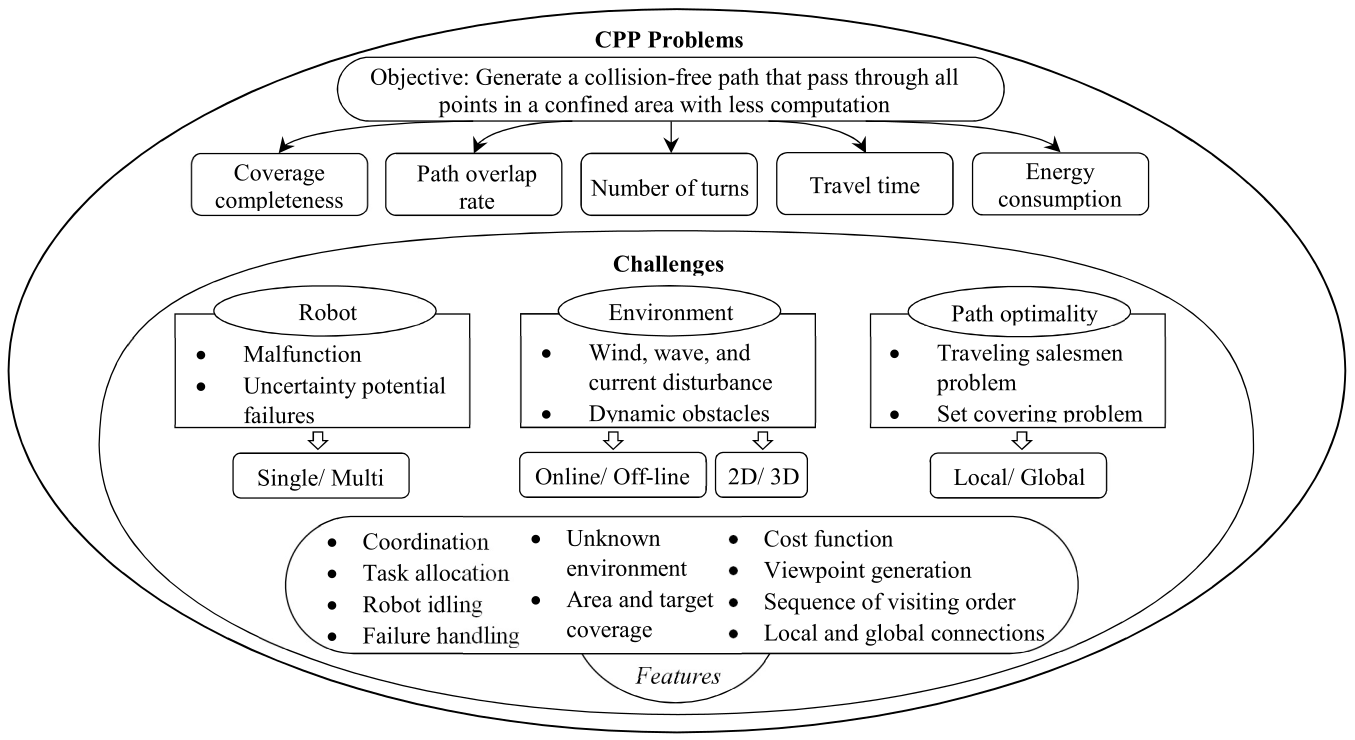
\includegraphics[width=\textwidth]{Images/general/overview_of_CPP.png}
    \caption{The objective and challenges in coverage path planning (CPP) problems.}
    \label{fig:overview_of_CPP}
\end{figure}

Over the years, researchers have developed a myriad of algorithms to address different aspects of path planning, ranging from basic algorithms to more advanced methodologies. CPP algorithms can be categorized into two approaches, classical algorithms, and heuristic-based algorithms. The summarized details of CPP algorithms according to the characteristics of the algorithms as stated in the paper \hyperlink{cite.main_review}{[2]} are classified as shown in (\autoref{fig:classifications_of_CPP}). 

\begin{figure}[htbp]
    \centering
    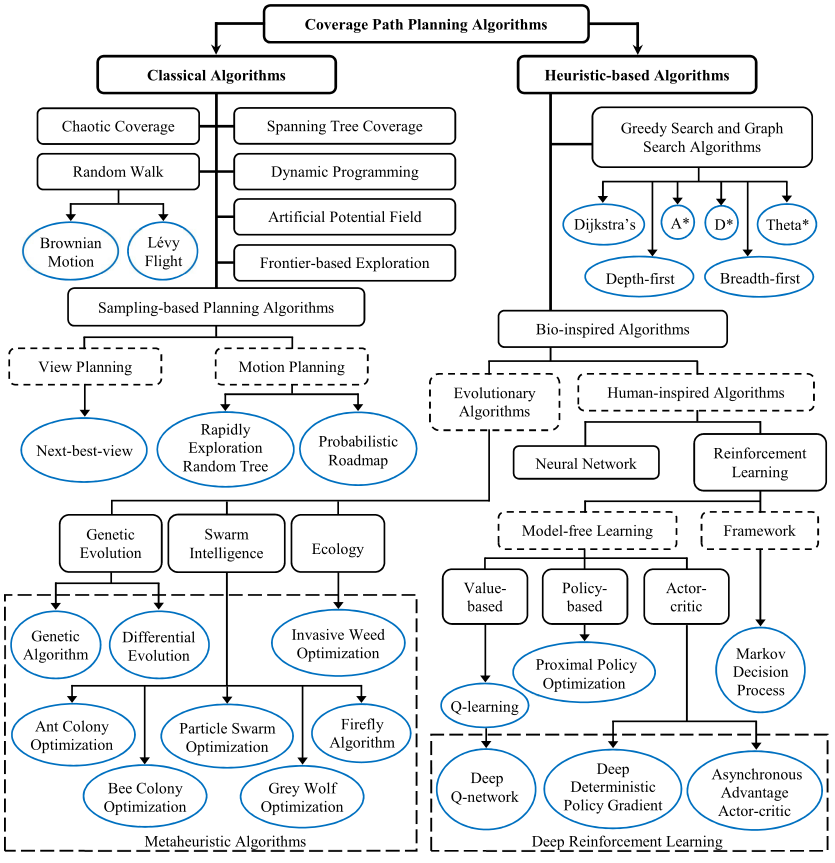
\includegraphics[height=22cm, width=\textwidth]{Images/general/general_classification.png}
    \caption{The classification of coverage path planning (CPP) algorithms.}
    \label{fig:classifications_of_CPP}
\end{figure}

\vspace{3mm}

Several algorithms relevant to coverage path planning for points or regions, which adhere to non-holonomic constraints with the objective of minimizing total route length, computational time, and energy consumption, are discussed below.


\subsection{Dubin's Path}

In the realm of geometric analysis and constrained path planning, the pioneering work of L.E. Dubins stands as a cornerstone, providing profound insights into the properties and characteristics of paths subject to curvature constraints. Dubins' seminal exploration, outlined in the paper \hyperlink{cite.dubins}{[1]}, lays a robust foundation for understanding the fundamental principles governing constrained path planning and provides critical insights into the properties of paths constrained by curvature.

\vspace{3mm}

At the core of Dubins' research lies the concept of R-geodesics, representing paths of minimal length under specified curvature constraints. This notion encapsulates the geometric essence of constrained paths, defining them as combinations of straight lines and circular arcs with a minimum radius of curvature, denoted as R. Dubins' theorem regarding the structure of R-geodesics in two dimensions provides a clear geometric understanding, asserting that such paths consist of no more than three segments, each comprising either a straight line or an arc of a circle with radius R. This theorem delineates the structure of minimal paths and imposes precise constraints on their composition, revealing the inherent simplicity of paths subject to curvature constraints.

\vspace{3mm}

Dubins rigorously proved the existence of R-geodesics using mathematical tools like Ascoli's theorem and concepts from E. Schmidt's proof of A. Schur's Lemma. These proofs confirm the theoretical existence of such paths and illuminate their analytical and geometric properties.

\vspace{3mm}

Dubins' work represents a significant milestone in the study of geometric analysis and constrained path planning, providing not only a solution to a specific geometric problem but also a methodological framework applicable to a broader class of problems in path planning and optimization. Therefore, many extensions of Dubins have been studied since then, integrating with other approaches to solve complex path planning problems. Due to its effectiveness towards curvature constraints and path length minimization, the Dubins path serves as a potential technique to inspire and inform further research into path planning algorithms for agricultural robots.


\subsection{Reeds-Shepp Paths}

Reeds-Shepp paths, introduced by J.A. Reeds and L.A. Shepp in the paper \hyperlink{cite.reeds}{[3]}, offers a flexible solution to optimal path planning for vehicles capable of moving forwards and backwards. Unlike Dubins paths, which only accommodate forward movement, Reeds-Shepp paths enhance maneuverability by incorporating reverse movements, doubling the range of possible maneuvers. This flexibility enables efficient navigation in complex environments, making them ideal for applications like robotics and autonomous vehicle navigation.

\vspace{3mm}

In agricultural robotics, Reeds-Shepp paths are particularly beneficial for tasks like weed removal, where precise navigation is essential. Their flexibility allows for efficient navigation through narrow spaces and around obstacles, reducing time and energy consumption. Reeds and Shepp's comprehensive analysis of Reeds-Shepp paths laid the foundation for subsequent research in optimal control and path planning, emphasizing the importance of considering a vehicle's full range of capabilities.





\subsection{Travelling Salesman Problem (TSP) with Neighborhoods} 

The Traveling Salesman Problem (TSP) represents a classic conundrum in optimization, challenging researchers to find the most efficient route for a salesman to visit a set of locations and return to the starting point while minimizing the total distance traveled. Renowned for its computational complexity and practical applications in logistics and route planning, the TSP has spurred numerous investigations into variants that more accurately reflect real-world scenarios.

\vspace{3mm}

One such variant, explored in the paper \hyperlink{cite.TSPN}{[4]}, introduces the concept of TSP with neighborhoods (TSPN). In this formulation, destinations are not singular points but rather areas or neighborhoods, complicating the problem by requiring the salesman to visit each neighborhood at least once without specifying exact points for each visit. TSPN is particularly relevant as it mirrors the challenge of navigating through regions (fields with weeds) rather than fixed points.

\vspace{3mm}

To address the challenges posed by TSPN, the paper introduces innovative approximation algorithms tailored to different types of neighborhoods, such as line segments or complex shapes described as "fat" regions. A notable contribution is the development of a constant factor approximation algorithm for neighborhoods represented as line segments, signifying a significant advancement in the field of geometric optimization.

\vspace{3mm}

A significant contribution of the paper is the m-guillotine method, which recursively subdivides the plane to approach a near-optimal solution. This method, along with key theoretical insights, underpins the algorithms' effectiveness in solving TSPN. However, it is essential to note that the TSPN problem is NP-hard, and the proposed algorithms provide only approximation solutions. While TSPN works with regions instead of points and strives to find the optimal solution, it does not explicitly consider the curvature constraints inherent in robotic path planning scenarios.











\subsection{Traveling Salesperson Problems for Dubins’ vehicle.}



After TSPN evolved from TSP, the challenges associated with optimal path planning for Dubins' vehicles, constrained by their minimum turning radius, have garnered significant attention. The paper \hyperlink{cite.TSP_with_dubins}{[5]} offers a thorough examination of these challenges and introduces innovative methodologies to overcome them.

\vspace{3mm}


At the core of this paper are two fundamental problems: the point-to-point shortest path problem (PTP) and the traveling salesperson problem (TSP) tailored for Dubins’ vehicles. These problems are crucial for developing algorithms capable of computing optimal or near-optimal paths for vehicles subject to nonholonomic constraints. the paper tackles the traveling salesperson problem (TSP) for Dubins’ vehicles, wherein the vehicle must visit a predefined set of locations in the most efficient route without revisiting any point. Acknowledging the computational complexity of exact solutions for larger point sets, the authors explore heuristic and approximation algorithms to efficiently approximate solutions.

\vspace{3mm}

The methodology outlined in the paper integrates rigorous mathematical frameworks and computational geometry to address the complexities of path planning for Dubins’ vehicles. By synthesizing Dubins constraints with the Traveling Salesperson Problem (TSP), the study offers a cohesive approach that bridges theoretical insights with practical solutions. this paper constitutes a significant contribution to the literature on path planning for nonholonomically constrained vehicles, paving the way for further advancements in navigating Dubins’ vehicles efficiently and effectively.











\subsection{Dubins Traveling Salesman Problem with Neighborhoods}

To address the challenges posed by regions in the Dubins Traveling Salesman Problem (DTSP), the paper \hyperlink{cite.DTSPN}{[6]} introduces a tailored formulation termed the Dubins Touring Regions Problem (DTRP). This novel approach aims to determine an optimal sequence of configurations for entering and exiting regions, all while minimizing the total path length. Unlike the conventional Traveling Salesman Problem (TSP), which focuses on finding the shortest route visiting a set of points, the DTSPN involves regions or neighborhoods, necessitating the vehicle to access each region at least once. This problem holds significant relevance in various applications, including autonomous drone surveillance, delivery systems, and robotic exploration, where vehicles must efficiently traverse specified areas while adhering to nonholonomic constraints.

\vspace{3mm}

The proposed algorithm for solving the DTRP leverages local iterative optimization techniques, taking into account the unique dynamics of Dubins vehicles. It begins with an initial sequence of region visits derived from solving an Euclidean TSP (ETSP), which serves as a proxy for the region centers. The algorithm then iteratively refines the entry and exit configurations to minimize the total tour length.

\vspace{3mm}

A key aspect of the solution method is its decoupled approach, optimizing the heading and position of each entry point independently. This simplification, facilitated by mathematical techniques that project the problem into a more manageable form, allows for efficient local optimization. The algorithm iterates until no further improvements can be made or a termination criterion is met, incorporating strategies to escape local minima by adjusting vehicle headings and repositioning at region boundaries.

\vspace{3mm}

Empirical validation of the algorithm demonstrates its effectiveness and efficiency across various scenarios, including different region shapes and configurations, particularly in dense environments where regions are close together. Comparative analysis against existing evolutionary algorithms showcases the proposed method's ability to produce high-quality solutions with significantly reduced computational time, making it suitable for real-time applications on modest hardware, such as onboard computers in UAVs.

\vspace{3mm}

Despite its capability to generate near-optimal paths while adhering to the non-holonomic constraints, the algorithm exhibits notable drawbacks in terms of computational efficiency. For instance, computing a near-optimal path for 30 regions may require over a minute, and the algorithm's performance further deteriorates with an increasing number of points, especially when they are closely positioned. Moreover, the algorithm's limitation in considering the overlap of regions represents a critical drawback, as it fails to account for this aspect in real-world scenarios, thereby impacting the path planning accuracy and efficiency.




\subsection{DTSPN with Overlappped Regions}



The paper \hyperlink{cite.overlap}{[7]} introduces the Intersecting Regions Algorithm (IRA) to address the challenges posed by intersecting regions in DTSPN. By explicitly considering the overlap among regions, IRA offers a more comprehensive solution compared to traditional methods. It leverages sampling within intersecting regions to construct feasible tours for autonomous vehicles, resulting in optimized route selection and more efficient path planning.

\vspace{3mm}

Furthermore, IRA reduces the computational complexity associated with path planning by adopting a polynomially scalable algorithmic structure. This scalability ensures IRA's viability even in scenarios with numerous regions of interest, where computational resources are limited. Monte Carlo simulations validate IRA's practical utility, showcasing significant performance enhancements, particularly in scenarios with high degrees of region overlap. However, despite its advancements, IRA still encounters challenges when dealing with a large number of points and close proximity points. These limitations highlight avenues for further research and development to enhance the algorithm's robustness and efficiency in addressing complex DTSPN scenarios.








\subsection{Path planning in confined spaces}


Navigating narrow and complex environments presents challenges for non-holonomic vehicles. In the paper \hyperlink{cite.mapping}{[8]}, the authors propose a path planning method tailored to address these challenges, focusing on generating paths with continuous curvature to ensure smooth operation in confined spaces.

\vspace{3mm}

The proposed method adopts a two-phase planning approach combining global and local strategies for efficient navigation. In the first phase, the authors employ the RTR (Rotate-Translate-Rotate) planner, a variation of the Rapidly Exploring Random Tree (RRT) method. This planner generates paths consisting of straight movements and in-place turning, simplifying complex maneuvering for navigating constrained spaces.

\vspace{3mm}

In the second phase, the global path is refined using the TTS local planning procedure. This planner approximates the initial path with a sequence of paths adhering to the vehicle's curvature constraints, ensuring smooth and feasible trajectories. The TTS planner can generate paths with continuous curvature turns (CC-turns) and straight segments, offering flexibility adaptable to various environmental constraints.

\vspace{3mm}

The paper also emphasizes maintaining similarity between global and local trajectories to avoid sudden changes in the path and ensure smooth passage through narrow regions. Ultimately, the objective is to enhance the capabilities of autonomous vehicles to operate safely and efficiently in diverse scenarios, thereby improving their practicality for everyday use.


% \newpage

% \section{Literature Review for Obstacle Avoidance.}


\subsection{Random walk (RW) algorithms}

Random walk (RW) algorithms, commonly employed in path planning (CPP) tasks, offer a stochastic approach to obstacle avoidance in robotics. By mimicking the random movements observed in natural phenomena, RW algorithms enable robots to navigate environments while adapting obstacles. Although primarily designed for exploration and coverage, RW algorithms can effectively avoid obstacles by dynamically adjusting movement directions based on environmental cues. However, their effectiveness and efficiency in obstacle-rich environments is limited, as random movements could lead to inefficient navigation.

\subsection{Dynamic Programming}
Dynamic Programming (DP) offers a robust approach to Coverage Path Planning (CPP), efficiently optimizing coverage paths while considering factors like obstacles and turns. DP's advantage lies in its ability to handle overlapping sub-problems and exploit optimal substructure, making it suitable for generating globally coverage paths. By optimizing the sequence of segments and connections, DP algorithms construct shorter and more efficient coverage paths, addressing challenges like coverage overlaps. However, scalability concerns arise with large-scale CPP problems, as DP algorithms require extensive computational resources and time to generate complete paths. 


\subsection{Artificial Potential Field (APF) Algorithm}

The artificial potential field (APF) algorithm is widely used for obstacle avoidance and navigation in Coverage Path Planning (CPP). By employing virtual repulsive forces around obstacles and attractive forces toward the goal, the APF algorithm guides robots while ensuring a safe distance from obstacles. The susceptibility of the artificial potential field (APF) algorithm to local optima presents a notable challenge, potentially leading to the entrapment of robots in specific environmental regions. Additionally, the algorithm's computation is resource-intensive, particularly in generating potential fields for the entire environment. Moreover, robots will experience repulsive forces not only from the front but also from the sides and behind obstacles, further complicating navigation.

\subsection{Spanning Tree Coverage Algorithms in coverage path planning}

Spanning Tree Coverage (STC) algorithms as mentioned in the paper \hyperlink{cite.spanning_tree}{[12]} offer a systematic approach to coverage path planning by dividing the workspace into disjoint cells and constructing spanning trees within them. This method allows robots to navigate around or through obstacles for comprehensive coverage. Initially, the workspace is partitioned into cells, and spanning trees are formed within these cells to guide robot movement. However, challenges arise when obstacles obstruct sub-cells within mega-cells, impeding complete coverage.

\vspace{3mm}

To mitigate this issue, researchers have proposed extensions like the full-STC algorithm, enabling robots to maximize area coverage by addressing free sub-cells. Optimization efforts focus on improving cell assignment and task distribution. Auction-based algorithms and wall-following approaches facilitate obstacle navigation within mega-cells. Yet, minimizing backtracking and increasing coverage rates remain priorities, especially in scenarios with partially occupied mega-cells.

\vspace{3mm}

Recent advancements aim to enhance energy efficiency and fault tolerance in real-world applications. Hybrid approaches combining frontier-based exploration with STC algorithms reduce energy consumption. Nonetheless, challenges persist, such as workload distribution imbalance. Despite these challenges, STC algorithms offer a systematic and efficient solution, particularly in environments with static obstacles. However, for large fields and complete coverage, discretization of the complete field is not feasible and optimal due to computational constraints and scalability issues.





\subsection{Sampling-Based Planning Algorithms for Obstacle Avoidance}

Sampling-based planning algorithms have become prominent tools for solving complex path planning problems in robotics, particularly in environments with numerous obstacles. These algorithms use random sampling to explore the configuration space, offering both heuristic and optimal solutions. Their probabilistic nature allows them to effectively handle the uncertainty and complexity inherent in real-world scenarios, making them suitable for applications requiring efficient navigation and obstacle avoidance. An overview of sampling-based planning algorithms is available in the paper cited as \hyperlink{cite.sampling_based_more_related}{[14]}.

\subsubsection{Probabilistic Roadmap (PRM)}

The Probabilistic Roadmap (PRM) algorithm constructs a roadmap by randomly sampling configurations within the robot's environment and connecting them with collision-free paths. This roadmap serves as a global map, enabling efficient path planning between start and goal configurations. While PRM is effective for static environments and provides a comprehensive exploration of the space, its random node placement can limit coverage near boundaries and obstacles, and it may incur high computational costs in densely populated environments.


\subsubsection{Randomized Potential Field (RPF)}

The Rapidly Exploring Random Tree (RRT) algorithm incrementally builds a tree by randomly sampling configurations and expanding the tree toward unexplored regions or towards the goal. RRT is suited for static environments due to its ability to rapidly explore the configuration space without needing a precomputed roadmap. However, while RRT efficiently finds feasible paths, the paths may not always be optimal. Variants like RRT* have been developed to improve path quality by providing asymptotically optimal solutions, addressing challenges in navigating through narrow passages and cluttered spaces.

\vspace{3mm}


However, sampling-based algorithms are not ideally suited for complete coverage path planning, as they are primarily designed for point-to-point navigation rather than comprehensive area coverage. Modeling non-holonomic constraints in coverage path planning presents additional challenges that necessitate alternative approaches. Implementing a sampling-based method for complete coverage by generating a roadmap for the entire environment is computationally intensive and impractical for large-scale environments.



\subsection{Greedy Search Algorithms in Coverage Path Planning}

Greedy search algorithms, such as Dijkstra's algorithm, make decisions based on the local optimal choice at each step, without considering global implications. For these approaches to find the goal point, a graph has to be generated before hand and shortest path will be ensured from that graph. This heuristic method is simple and fast but does not guarantee globally optimal solutions due to its short-term focus. In robotics, graph search algorithms like A*, D*, and Theta* are commonly used to plan and optimize coverage paths, employing strategies like boustrophedon motion or spiral patterns. These algorithms are crucial for obstacle avoidance, dynamically re-planning paths when encountering obstacles or blind spots to ensure continuous coverage. However, path searching in large grid maps poses computational challenges due to the vast search space, necessitating ongoing advancements to improve efficiency and reduce computation costs.


\subsubsection{Dijkstra's Algorithm in Coverage Path Planning}  

Dijkstra's algorithm is used to find the shortest path from a single source node to the goal node in a graph with non-negative edge costs. In coverage path planning (CPP), it helps optimize path sequences and minimize traversal costs, ensuring thorough coverage while avoiding obstacles. Applications include indoor navigation and optimizing coverage paths with minimal resource consumption. Despite its effectiveness. It will find the shortest path and is computationally expensive as compared to other graph search approaches.


\subsubsection{A* Algorithm in Coverage Path Planning}

The A* algorithm combines actual and estimated costs to determine the shortest path from a start node to a goal node, making it effective for CPP where minimizing cost is crucial. It has been used to optimize path sequences, reduce processing time, and ensure comprehensive coverage while avoiding obstacles. A* is valuable in CPP applications, balancing efficient pathfinding with comprehensive coverage, especially when tailored to address specific challenges in complex environments.


\subsubsection{Theta* Algorithm in Coverage Path Planning}

Theta* allows pathfinding in the graph, enabling more flexible and efficient navigation compared to other methods like A*. It is particularly useful for CPP in environments where precise path planning is essential. Practical applications include cleaning robots, where Theta* optimizes local backtracking paths to improve coverage time.


\vspace{3mm} 
 
The aforementioned graph search approaches are effective when the graph is predefined and the objective is to find the shortest path from source to goal. However, in coverage path planning, the objective shifts to covering the entire area. Prioritizing straight paths makes generating a comprehensive graph for the entire environment computationally expensive  and does not guarantee the generation of an optimal or near-optimal graph over the complete region that ensure the near optimal path. 



\subsection{Combinatorial Planning Techniques}

Combinatorial planning techniques emerged as a response to the need for efficient and systematic
methods to navigate robots through complex environments cluttered with obstacles. As robotics
applications expanded into domains such as manufacturing, logistics, and exploration, the
demand for reliable path planning algorithms became increasingly pronounced. Traditional
approaches often struggled to cope with the intricacies of real-world environments, leading to
the development of combinatorial planning techniques.

\vspace{3mm} 
 

These techniques were invented to provide a structured framework for path planning by
discretizing the continuous configuration space into a graph-based representation. By breaking
down the problem into manageable components, combinatorial planning methods aimed to
overcome the challenges posed by obstacles and non-trivial workspace geometries. They offered a systematic way to explore the configuration space, enabling robots to navigate from an initial
pose to a desired goal while avoiding collisions. Key algorithms in this field include Visibility Graphs, Voronoi Diagrams, Exact Cell Decomposition, and Approximate Cell Decomposition, each tailored to address specific challenges and requirements.


\subsubsection{Visibility Graphs}

Visibility Graphs are a fundamental combinatorial planning technique used to navigate robots through environments cluttered with obstacles. This method constructs a graph by connecting the initial and goal configurations through vertices representing the obstacles. By leveraging visibility between vertices, Visibility Graphs systematically derive collision-free paths that optimize for efficiency and optimality. The paths generated inherently minimize distance and traversal time, leading to efficient navigation. While Visibility Graphs are robust and produce optimal paths, their computational overhead in complex environments with numerous obstacles remains a limitation.


\subsubsection{Voronoi Diagrams}

Voronoi Diagrams offer a distinct approach in combinatorial planning by generating collision-free paths through a tessellation of space into regions based on proximity to a set of points. Each region, or Voronoi cell, encompasses locations closer to its defining point than to any other. This partitioning provides valuable insights into potential navigation paths, offering robustness to complex environments with irregular obstacle geometries. Voronoi Diagrams prioritize paths that maintain safe distances from obstacles, enhancing safety. However, they may produce sub-optimal paths in intricate environments and involve significant computational costs in construction.


\subsubsection{Exact Cell Decomposition}

Exact Cell Decomposition decomposes the free configuration space into trapezoidal cells using vertical side segments from polygon vertices, simplifying the path planning process by focusing on individual regions. This approach ensures comprehensive exploration of the environment, making it suitable for applications like surveillance, mapping, and search-and-rescue missions. It offers increased clearance from obstacles and scalability to varying environment sizes. However, it tends to produce sub-optimal paths in complex obstacle configurations and is limited to polygonal obstacles, which restricts its utility in non-polygonal environments.


\subsubsection{Approximate Cell Decomposition}


Approximate cell decomposition offers a grid-based approach to path planning, dividing the configuration space into fixed or variable-sized grids and labeling each cell as free or occupied to represent free space and obstacles. The advantage of this method is its flexibility in handling obstacles of various shapes and sizes, allowing for greater versatility in navigating complex environments. Pre-generated grids reduce computational time during path planning, resulting in faster planning times compared to methods that require graph generation and search.

\vspace{3mm}

However, approximate cell decomposition has limitations. It will struggle with dynamic obstacles, needing frequent grid updates to accommodate environmental changes, which increases complexity and decreases efficiency. Fixed resolution constraints can limit its ability to represent fine-grained details, affecting accuracy and precision in intricate environments. Additionally, representing a very large region with high-resolution grids will be computationally expensive, as maintaining detailed obstacle and free space information increases computational overhead.

\subsection{State Lattice Planning}
State lattice planning as stated in \hyperlink{cite.state_lattice}{[15]} is a systematic method designed to generate feasible paths for robots navigating continuous environments with non-holonomic constraints. This approach involves discretization, where the continuous space is divided into a finite number of nodes, each representing a possible robot pose, accounting for both position and orientation. The process continues with node expansion, ensuring that each node adheres to the robot's physical constraints, making the generated states traversable. This is followed by connectivity, where expanded states are connected to form a graph that represents possible paths through the environment. Path generation utilizes a graph search algorithm to identify the optimal path from the start to the goal state following the non-holonomic constraints.

\vspace{3mm}

State lattice planning offers several key advantages for robotic navigation. It ensures completeness, guaranteeing that if a feasible path exists, the algorithm will find it. This method also provides an optimal solution by identifying the shortest path, minimizing travel distance and time. Additionally, state lattice planning can dynamically replan paths in real-time in response to environmental changes or new constraints, enhancing the robot’s adaptability and safety in dynamic scenarios. 

\vspace{3mm}

Despite its advantages, state lattice planning has the limitation that generating an approximate straight path often necessitates a dense tree of nodes. This significantly increases computational time, particularly in environments with numerous obstacles. Thus, while state lattice planning provides a robust framework for path planning, its effectiveness can vary based on the specific requirements and constraints of the robotic application.

\vspace{3mm}


In addition to these classical techniques, several heuristic algorithms address exploration and coverage problems. These include boustrophedon motion, internal spiral algorithms, Voronoi partition approaches, Brick and Mortar algorithms, to name a few. Each algorithm offers unique strategies and approaches to address specific challenges in exploration and coverage, contributing to the diverse landscape of combinatorial planning in robotics.



\subsection{Other Classical and Heuristic Algorithms.}

In the realm of path planning for robotics, evolutionary algorithms (EAs) and human-inspired approaches have garnered considerable attention for their ability to find optimal or near-optimal solutions to complex optimization problems. One prominent example is Genetic Algorithms (GA), a metaheuristic inspired by natural genetic evolution, which has been extensively employed in solving various path planning problems. GA operates by iteratively evolving a population of potential solutions through mechanisms like crossover and mutation, eventually converging towards a solution that meets predefined criteria.

\vspace{3mm}


While GA offers the advantage of global search capability, it often suffers from poor stability and high computation time, particularly in scenarios with large search space complexity. To address these limitations, researchers have proposed enhancements such as multi-objective GA and hybrid approaches combining GA with other techniques like Dynamic Programming (DP) or simulated annealing. These adaptations aim to improve convergence speed and solution quality while mitigating the computational burden.

\vspace{3mm}


Another noteworthy EA is Differential Evolution (DE), which offers advantages such as quick convergence and robustness. DE operates by iteratively generating trial vectors through mutation, recombination, and selection processes, making it particularly suitable for optimization problems with complex search spaces. Researchers have explored various modifications to DE, such as combining it with roulette and multi-neighborhood operations, to enhance its performance in path planning tasks.

\vspace{3mm}


In addition to EAs, swarm intelligence algorithms have gained prominence for their ability to emulate collective behavior observed in natural systems. Particle Swarm Optimization (PSO), Ant Colony Optimization (ACO), and Bee Colony Optimization (BCO) are notable examples of swarm intelligence algorithms applied to path planning. These algorithms leverage the collective intelligence of swarm agents to efficiently explore and optimize paths in complex environments. However, they may face challenges such as local optima trapping and slow convergence rates, prompting researchers to propose enhancements like distributed algorithms and improved pheromone updating rules.

\vspace{3mm}


On the other hand, human-inspired algorithms, such as neural networks and reinforcement learning (RL), draw inspiration from the workings of the human brain to optimize decision-making processes in path planning. Neural networks, including feedforward and convolutional architectures, have been utilized to learn complex mappings between sensory inputs and actions, enabling robots to navigate and plan paths in dynamic environments. Reinforcement learning, a subset of machine learning, allows agents to learn optimal behaviors through trial-and-error interactions with the environment. RL algorithms like Q-learning and Deep Q-Networks (DQN) have shown promise in optimizing path planning tasks, albeit with challenges related to convergence speed and scalability.

\vspace{3mm}


Despite their potential, evolutionary and human-inspired approaches will not be suitable for scenarios requiring real-time path planning or where computational efficiency is paramount. These methods typically involve iterative optimization processes that will incur significant computation time, making them less practical for time-sensitive applications. Thus, while these approaches offer valuable insights into path planning optimization, their adoption may depend on the specific requirements and constraints of the robotics task at hand.


\subsection{Inspiration drawn from existing approaches}

From the approaches discussed in the literature review, some are efficient in computation time using heuristics but do not follow non-holonomic constraints. Others follow non-holonomic constraints but do not prioritize naturally straight paths, while some algorithms focus solely on path optimization, resulting in high computational times for generating the optimal path. Hence, it is clear that none of the above approaches can be used directly for our problem statement. A new approach was needed that reduces computational time using heuristics, adheres to non-holonomic constraints, and prioritizes straight paths.

\vspace{3mm}

To develop an efficient and effective path planning algorithm for coverage path planning, inspiration was drawn from state-of-the-art approaches to build and enhance the algorithm. They are listed as follows:

\begin{itemize}[noitemsep]
    \setlength{\itemsep}{7pt}
    \item Implementation of a vision cone approach to prioritize linear paths.
    \item Application of a combined criterion to select the optimal point within the vision cone.
    \item Computing the centroids from the intersection of the union of multiple regions to derive points from regions.
    \item Modeling the non-holonomic constraints in the global path to closely resemble the local path.
    \item Utilization of the Dubins open traveling salesman problem to determine the shortest path across multiple points.
    \item Implementation of decoupled Dubins constraints following the generation of linear paths.
    \item Adoption of a grid-based methodology for obstacle representation, while employing continuous space for free space.
    \item Leveraging state lattice planning to construct a graph that adheres to non-holonomic constraints.
    \item Implementation of the A* algorithm to ascertain the optimal path from the generated graph.
    \item Application of Reeds-Shepp paths to determine the shortest route between two points in the local path for efficient weed coverage.
\end{itemize}
% \newpage


% \section{Problem Statement}

We consider a robotic scenario wherein a four-wheel robot equipped with a mechanical CNC-inspired system for extraction operates within a defined area. The robot, characterized as non-holonomic, integrates the mechanical system beneath it, enabling movement along the x and y directions by approximately 60 cm, and vertically until ground contact. Due to its non-holonomic nature, the robot imposes kinematic constraints on turning, enforcing a minimum turning radius of 2 meters.

\vspace*{6mm} 


The operational environment comprises grass fields assumed to be uniform without any slopes (z=0), covering a real area of 120x90 square meters. Weed distribution within this area is heterogeneous, with approximately 60 percent of points clustered following a Gaussian distribution with varying variances. Weed positions are obtained via drone-based data collection, utilizing a deep learning model to identify weed locations. This dataset serves as the basis for complete coverage path planning.

\vspace*{6mm} 


Given the robot's mechanical implementation width of 60 cm, the operational region is discretized into points with each point representing an area of 30 cm, facilitating path planning optimization. The robot's velocity is constrained to 0.8 m/s on straight paths and 0.4 m/s on curved paths.

\vspace*{6mm} 


The primary objective of this research is to develop a path planning algorithm capable of covering all weed points within the designated area while adhering to the robot's non-holonomic constraints. Additionally, the algorithm aims to generate paths that approximate straight lines where feasible, ensuring comprehensive coverage of all points.

\vspace*{6mm} 

The objectives of the proposed algorithm include:

\begin{itemize}
    \item \textbf{Realistic Path Generation:} Develop paths that mimic natural movement patterns, enhancing operational realism.
    \item  \textbf{Computational Efficiency:} Minimize processing time and resources required for path planning.
    \item  \textbf{Energy Conservation:} Optimize energy consumption during path execution, enhancing overall operational efficiency.
    \item  \textbf{Field Operation Efficiency:} Facilitate efficient field operations, reducing time spent on weed detection and removal processes.
\end{itemize}

The algorithm should prioritize finding the shortest path distance to cover all weed points effectively while meeting the aforementioned objectives. The algorithm's performance will be evaluated based on the time taken to generate paths, the distance covered, and the energy consumed during path execution.

\vspace*{6mm} 


% \newpage


% \section{Experimental Setup}

\subsection{Environment}
The environment for our coverage motion planning algorithm is situated in a grass field characterized by small grass uniformly distributed across the area. The grass field is representative of typical agricultural settings, where weed management is essential for maintaining crop quality and productivity. As the grass matures, it is common for various unwanted plants, particularly weeds, to grow sporadically throughout the field. Our primary focus in this study is on the removal of Rumex (commonly known as dock weeds), which pose a significant challenge to farmers. However, the algorithm can be adapted to target other types of weeds based on specific requirements, the only that change would be the detection system to identify the target weed.

\subsection{Importance of Weed Removal}
Importance of Weed Removal
We are concentrating on Rumex plants due to their detrimental impact on agricultural productivity and livestock health. Although Rumex plants are not inherently toxic, their presence in cattle feed can adversely affect the quality of milk production. Ensuring the purity of grass fed to cattle is crucial for producing high-quality, bio milk, which is not only more beneficial for human consumption but also promotes better health and well-being of the cattle. Pure grass feed leads to higher nutritional value in milk, contributing to improved dairy products. Therefore, effective weed management, particularly the removal of Rumex plants, is essential for maintaining the quality and productivity of grass fields.


\vspace*{6mm} 


Traditionally, farmers have resorted to manually removing these weeds, a labor-intensive and time-consuming process. Manual removal becomes particularly arduous in large fields, imposing significant physical strain on farmers and limiting the efficiency of weed management. Automating this process with robotic systems offers a promising solution to enhance agricultural practices and improve farmers' quality of life.

\vspace*{6mm}

\subsection{The Robot}

\subsubsection{Overview}

To efficiently remove weeds from the grass field, we employ a robust, four-wheeled robot specifically designed for this task. This section provides an in-depth look at the robot's external and internal features, highlighting the components that enable it to navigate the field and execute precise weed extraction.

\subsubsection{External Features}

The robot features a four-wheeled design, ensuring stability and effective maneuverability across uneven terrain. The choice of a four-wheeled configuration is crucial as it supports the internal weed extraction system, which occupies most of the internal space. The wheels are equipped with treads suitable for grass fields, providing the necessary traction and mobility.

\vspace*{6mm}

\textbf{Localization and Orientation:} For accurate positioning and orientation in the open field, the robot is equipped with two Real-Time Kinematic (RTK) GPS systems. RTK GPS technology is ideal for this environment, offering centimeter-level accuracy in localization, which is essential for precise navigation and weed targeting.

\vspace*{6mm}


\textbf{Vision System:} The robot incorporates two strategically placed cameras. The front-facing camera is oriented towards the ground, scanning for weeds ahead of the robot. This early detection allows the local planner to adjust the robot's path accordingly, ensuring efficient navigation and weed targeting. The second camera is mounted at the bottom center of the robot, directly above the extraction mechanism. This camera provides an accurate view of the weed's position beneath the robot, facilitating precise extraction.


\subsubsection{Internal Features}

The internal mechanism of the robot is crucial for the precise and efficient removal of weeds. It comprises several key components: a processing unit, a battery system, and the main weed extraction system.


\vspace*{6mm}


\textbf{Processing Unit: } The processing unit serves as the brain of the robot, orchestrating the various functions and ensuring smooth operation. It processes data from the cameras and GPS systems, making real-time decisions to control the navigation and extraction processes. The unit is equipped with advanced algorithms for path planning, weed detection, and tool control, enabling the robot to perform its tasks autonomously and efficiently.


\vspace*{6mm}

\textbf{Battery System: }
The robot is powered by a robust battery system designed to provide sufficient energy for extended field operations. The battery pack is engineered for easy replacement, ensuring minimal downtime and continuous operation. This power system supports all onboard electronics, including the processing unit, cameras, GPS, and the weed extraction mechanism.


\vspace*{6mm}


\textbf{Weed Extraction System: }
The heart of the weed removal process is the weed extraction system, inspired by CNC machine technology. This system features two moving rails that allow the internal extraction mechanism to move in both the x and y directions. Controlled by the processing unit, these rails provide precise positioning capabilities. The extraction mechanism can move approximately 60 cm in both the x and y directions, covering a significant area beneath the robot. Once a weed is detected, the system moves the tool directly above the weed. The mechanical tool is then lowered in the negative z direction to engage the weed.

\vspace*{6mm}

The extraction tool is designed with sharp implements and rotates at high speed to destroy the weed effectively. This rotation ensures that the weed is thoroughly eradicated and cannot regrow. After destroying the weed, the remnants are left on the field, eliminating the need to carry them, which would otherwise burden the robot. The robot’s internal system, with its 60 cm movement range in both directions, allows for efficient navigation. Each detected weed point can be associated with a circular region within which the robot can maneuver to remove the weed. This approach not only aids in accurate weed extraction but also facilitates efficient path planning. By considering these regions, the planning algorithm can optimize the robot's path to cover all weed points effectively.

\vspace*{6mm}

\textbf{Adaptive Regions and Uncertainty Management: }
The regions around each weed point also serve to manage uncertainty in weed detection. If the position of a weed is detected with less accuracy, the associated region can be adjusted accordingly. A larger uncertainty reduces the size of the region to ensure the robot remains closer to the center, enhancing the likelihood of successful extraction. This adaptive approach allows the robot to handle variations in detection accuracy, maintaining high efficiency and precision in weed removal. The robot's internal features are meticulously designed to support the complex task of weed removal. The combination of precise movement capabilities, robust processing power, and adaptive region management ensures that the robot can effectively and efficiently eradicate weeds from the grass field.

\subsection{Constraints}

With a comprehensive understanding of the robot's capabilities and features, it is essential to delve into the constraints that arise due to its mechanical system and the nature of the field in which it operates. These constraints significantly influence the development of an effective motion planning algorithm.

\vspace*{6mm}

\textbf{Non-Holonomic Nature:}
The robot is equipped with four regular wheels, limiting its movement capabilities. Unlike holonomic robots, which can move in any direction, our robot cannot move sideways. It is constrained to forward and backward movements and must make turns to change its direction. This non-holonomic nature adds a layer of complexity to the motion planning algorithm, as it must account for the robot's inability to change its heading instantaneously.

\vspace*{6mm}

\textbf{Turning Radius:} The robot has a minimum turning radius of 2 meters, meaning it cannot make sharp turns. This constraint necessitates careful planning to ensure the robot can navigate around obstacles and reach all designated weed points without making turns that exceed its turning capabilities.

\vspace*{6mm}

\textbf{Speed Variations:} The robot's speed must be carefully regulated to prevent damage to the grass and ensure precise weed removal. When moving in a straight path, the robot operates at a velocity of 0.8 m/s. However, when making a turn, the velocity is reduced to 0.4 m/s to maintain the 2-meter turning radius. This adjustment helps in maintaining stability and accuracy during turns, which is critical for avoiding collateral damage to the grass and ensuring efficient weed extraction.

\vspace*{6mm}

\textbf{Kinematic Constraints:} Given its non-holonomic nature and the minimum turning radius, the robot cannot change its heading angle at a specific position. Instead, it requires a certain amount of space to turn and align itself in the desired direction. These kinematic constraints must be factored into the motion planning algorithm to ensure smooth and feasible navigation across the field.

\vspace*{6mm}

\textbf{Field Constraints:} The field is covered with grass and scattered weeds, particularly the rumex plants. The random distribution of weeds means the robot must navigate the entire field efficiently to locate and remove all weeds. The algorithm must account for this scattered distribution and plan paths that ensure comprehensive coverage without unnecessary overlaps.


\vspace*{6mm}



With a clear understanding of the robot's constraints, we can now proceed to develop a motion planning algorithm that leverages these constraints to ensure comprehensive and efficient weed removal. By integrating considerations for non-holonomic movement, adaptive speed control, optimized coverage, obstacle avoidance, and environmental adaptability, the algorithm will facilitate the robot's autonomous operation, making the weed removal process more efficient and reducing the burden on farmers. This strategic approach not only enhances the robot's performance but also contributes to maintaining the health of the grass and improving the overall quality of the field.

























\subsection{Remnants}


Benefits of Robotic Weed Removal
Deploying robots for weed removal in grass fields presents several advantages:

Increased Efficiency: Robots can operate continuously and systematically cover large areas, ensuring thorough removal of unwanted plants without fatigue.
Labor Savings: Automating weed removal reduces the need for manual labor, freeing farmers to focus on other essential tasks and reducing physical strain.
Precision: Advanced sensors and algorithms enable robots to identify and target specific weeds, minimizing damage to the surrounding grass and ensuring effective weed management.
Health Benefits: By eliminating the need for manual weed removal, farmers can avoid the physical exertion and potential health risks associated with prolonged exposure to outdoor conditions and repetitive movements.
Enhanced Livestock Health: Ensuring the purity of grass feed leads to healthier cattle, which in turn produce higher-quality milk, enhancing overall dairy production.


Experimental Objective
The primary objective of our experimental setup is to develop and validate a coverage motion planning algorithm that enables robots to efficiently navigate and manage weed removal in grass fields. By leveraging advanced robotic technology, we aim to automate the process of identifying and removing Rumex plants, ultimately improving agricultural productivity and promoting sustainable farming practices.

Methodology
The experimental setup involves the following key steps:

Field Analysis: Detailed mapping of the grass field to identify the distribution of grass and Rumex plants.
Algorithm Development: Creating a coverage motion planning algorithm tailored to navigate the field and target Rumex plants for removal.
Robotic Implementation: Equipping robots with necessary sensors and tools to detect and remove weeds, followed by field testing to ensure operational efficiency.
Performance Evaluation: Assessing the effectiveness of the robotic system in terms of coverage, weed removal accuracy, and operational efficiency.
By addressing the challenges of weed management through robotic automation, we aim to revolutionize agricultural practices, making farming more sustainable, efficient, and farmer-friendly. This innovative approach not only enhances the productivity of grass fields but also contributes to the overall well-being of livestock and farmers alike.
















Integrating Constraints into Motion Planning
Understanding the mechanical and field constraints is crucial for developing an effective coverage motion planning algorithm. These constraints guide the design of the algorithm to ensure it is practical and feasible under real-world conditions.

Path Planning with Non-Holonomic Constraints: The algorithm must plan paths that respect the robot's non-holonomic nature. This involves generating smooth, continuous paths that the robot can follow without needing to make sharp turns. Techniques such as Dubins curves, which are designed for non-holonomic vehicles, can be employed to create feasible paths that the robot can navigate.

Adaptive Speed Control: Incorporating variable speed control into the algorithm allows for safe and efficient navigation. The robot should move faster in straight paths to cover more ground quickly and slow down during turns to maintain stability and precision. This adaptive speed control also helps in preventing damage to the grass, ensuring that the robot's operations are minimally invasive.

Coverage Optimization: The algorithm should optimize the coverage pattern to ensure that all weeds are detected and removed efficiently. By considering the robot's 60 cm movement range in both directions, the algorithm can plan paths that cover larger areas without unnecessary backtracking. This optimization reduces the total time and energy required for weed removal.

Obstacle Avoidance and Navigation: The algorithm must include robust obstacle avoidance capabilities to navigate around natural terrain features and any unforeseen obstacles. This ensures the robot can continue its operation smoothly without interruptions.

Handling Environmental Variability: To ensure reliable performance under varying environmental conditions, the algorithm can incorporate sensor feedback to adjust the robot's path and speed in real-time. This adaptability enhances the robot's resilience and operational efficiency.
% \newpage

% \chapter{Methodology}

The main algorithm is comprised of two primary steps: data preprocessing and the behavior algorithm. In the data preprocessing phase, regions are converted into points by computing the centroids of their overlaps. The behavior algorithm phase utilizes these computed points to generate the complete path.

\section{Data Preprocessing}


Data preprocessing is a pivotal step in the research methodology, especially in the context of coverage path planning for weed removal in agricultural fields. This section delineates the comprehensive preprocessing procedures employed to ensure the precision and efficacy of the data used in the subsequent analysis.

\vspace{3mm}  


\textbf{Data Acquisition: }
The initial phase of preprocessing involves the acquisition of data pertaining to the weed positions within the field. This data collection is facilitated through the use of a drone for pinpointing the locations of weeds. The drone performs a systematic survey of the field, capturing high-resolution images to detect weed positions. The resultant data is then utilized as input for the coverage path planning module. Due to the developmental status of the drone, the current implementation involves manual data acquisition using a real-time kinematic GPS (RTK) system. The RTK system offers centimeter-level accuracy in pinpointing weed locations, which, for the purpose of this research, is considered sufficiently precise. 

\vspace{3mm}  


\textbf{Handling Data Uncertainty: }
In a practical scenario, the drone's output would include positional data of weeds along with an associated uncertainty measure, reflecting the inherent imprecision of the system. However, given the reliance on RTK data for this research phase, we assume perfect positional accuracy. This uncertainty measure will be used to define the regions of influence for each weed, ensuring that the coverage path planning algorithm accounts for the imprecision in the data. 


\vspace{3mm}  


\textbf{Region Definition and Overlap Management: } When data points from the drone indicate weed positions, these points often come with overlapping regions due to the growth patterns of weeds like Rumex, which tend to cluster.

\vspace{3mm}  


Overlap Reduction: To address overlaps, the preprocessing algorithm calculates the centroids of overlapping regions. Points within overlapping regions are consolidated to avoid duplication, ensuring that each weed cluster is represented by a single centroid. This consolidation reduces redundancy and enhances the efficiency of the coverage path planning.

\vspace{3mm}  


Non-Overlapping Weeds: For weeds whose regions do not overlap with others, the center of each weed is directly considered as a centroid. This step ensures that isolated weeds are accurately accounted for in the data set. The centroids of both overlapping and non-overlapping regions can be visualized in the \autoref{fig:overlape}. The green points represent the weeds, green circles represent the region of the weeds, and the red points represent the centroids of the regions. 

% selected field region.
\begin{figure}
    \centering
    \begin{tabular}{cc} 
        \begin{subfigure}{0.5\textwidth}
            \centering
            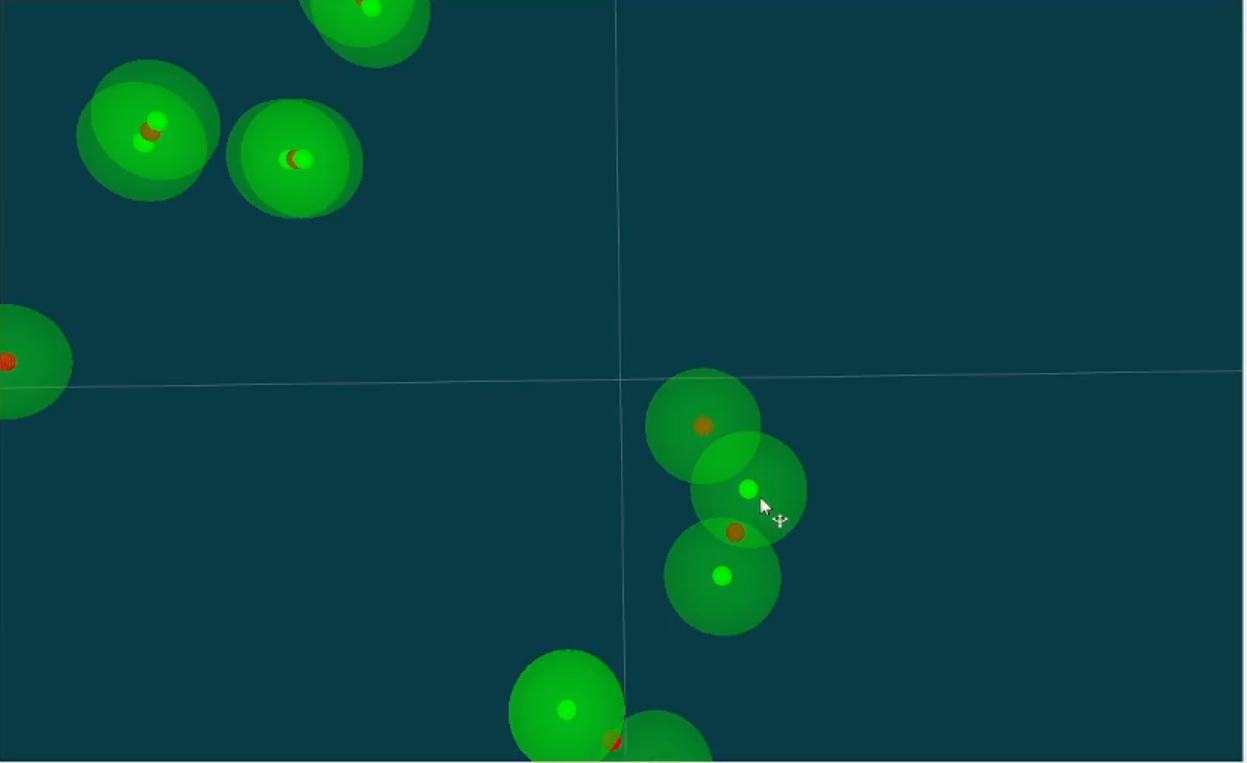
\includegraphics[width=\textwidth]{Images/Algorithm_no_obs/Centroid_1.png}
            % \caption{Selected Field Region}
        \end{subfigure} 
        &
        \begin{subfigure}{0.5\textwidth}
            \centering
            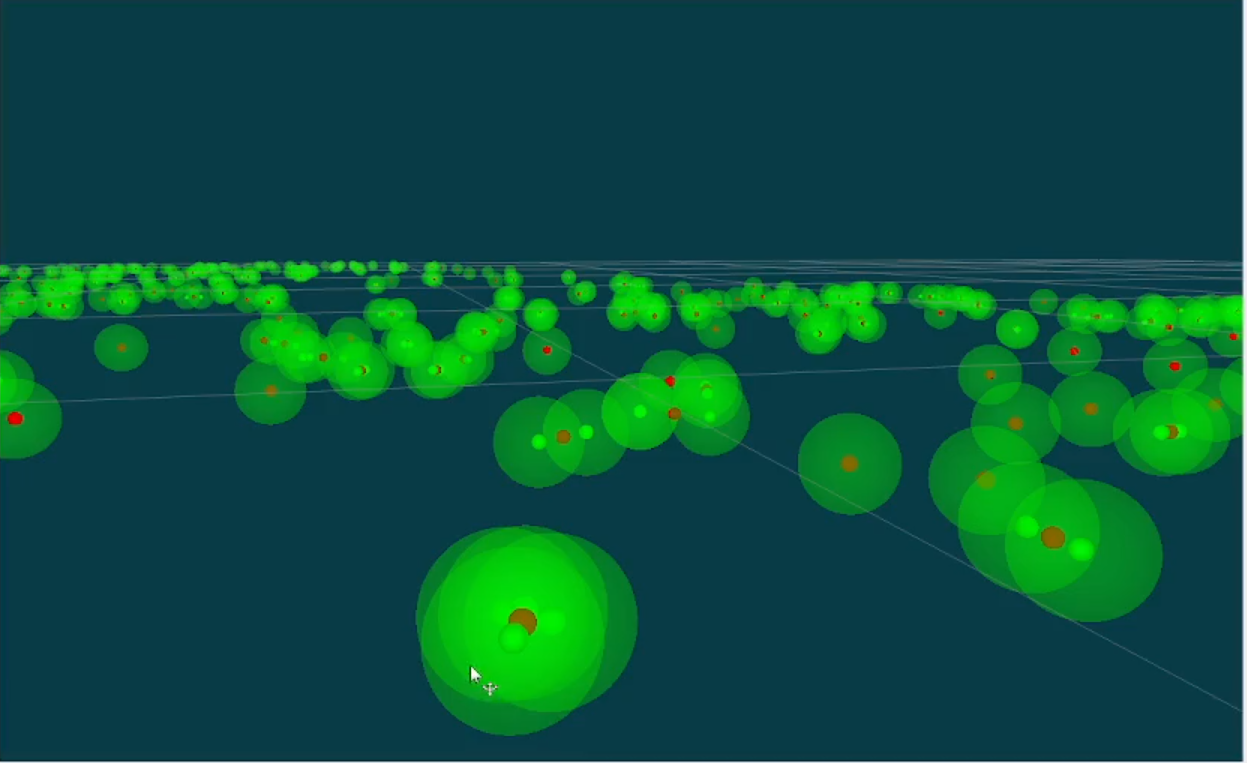
\includegraphics[width=\textwidth]{Images/Algorithm_no_obs/Centroid_2.png}
            % \caption{Points in the Region (Green)}
        \end{subfigure}
    \end{tabular}
    \caption{Centroids of overlapped regions.\label{fig:overlape}} 
\end{figure}

\vspace{3mm}  


\textbf{Data Integration and Optimization: }
By processing the data to identify centroids and manage overlaps, we achieve a significant reduction in the total number of points. Preliminary results indicate a reduction of at least 40\% in the number of data points, optimizing the dataset for coverage path planning. This reduction not only minimizes the total traversal length required for weed removal but also conserves energy and reduces redundant revisits.

\vspace{3mm}  


The processed data is then fed into the coverage path planning module, which utilizes the optimized set of points to devise an efficient path for weed removal, ensuring comprehensive coverage with minimal resource expenditure. The following figure illustrates the data preprocessing workflow, highlighting the steps taken to transform raw positional data into an optimized dataset ready for coverage path planning.

\vspace{3mm}  



This preprocessing approach ensures that the data fed into the coverage path planning algorithm is both accurate and efficient, laying a robust foundation for effective weed removal operations in agricultural fields.


% \newpage


% 
\subsection{Algorithm Description}




\section*{Data Preprocessing}


\subsection*{Region Definition and Overlap Management}

Given the robot’s extraction width of 60 cm, the field is divided into fixed regions. When data points from the drone indicate weed positions, these points often come with overlapping regions due to the growth patterns of weeds like Rumex, which tend to cluster.

Let:

\begin{itemize}
    \item $\mathbf{R}_i$ represent the region associated with data point $\mathbf{p}_i$.
    \item $\mathbf{C}$ be the set of centroids representing consolidated weed clusters.
\end{itemize}

\textbf{Overlap Reduction}

To address overlaps, the preprocessing algorithm calculates the centroids of overlapping regions. Points within overlapping regions are consolidated to avoid duplication, ensuring that each weed cluster is represented by a single centroid.

Let:

\begin{itemize}
    \item $\mathbf{O}_{ij}$ denote the overlap region between regions $\mathbf{R}_i$ and $\mathbf{R}_j$.
    \item $\mathbf{C}_k$ be the centroid representing the consolidated cluster of overlapping regions.
\end{itemize}

The centroid $\mathbf{C}_k$ can be calculated as the intersection of the overlapping regions:
\[
\mathbf{C}_k = \bigcap \mathbf{O}_{ij}
\]


\newpage

\section*{Vision Cone Strategy}

To effectively prioritize straight paths while minimizing computational complexity and time, we employ a vision cone mechanism for the robot. This vision cone is mathematically defined by two lines extending from the robot at a fixed angle and distance range.

Let:

\begin{itemize}
    \item $\theta$ be the angle of the vision cone.
    \item $d_{\text{min}}$ be the minimum distance of the vision cone.
    \item $d_{\text{max}}$ be the maximum distance of the vision cone.
    \item $\mathbf{p}_r$ be the current position of the robot.
    \item $\mathbf{h}_r$ be the heading direction of the robot.
\end{itemize}

The vision cone angle $\theta$ is determined by the robot’s minimum turning radius $R$. For instance, for a robot with a minimum turning radius of 2 meters, the angle of the cone on either side is set at 11 degrees:
\[
\theta = \pm11^\circ
\]

The distance range of the vision cone is defined by $d_{\text{min}}$ and $d_{\text{max}}$, where $d_{\text{min}}$ ensures that points too close to the robot are ignored, and $d_{\text{max}}$ sets the farthest point considered. For this scenario, the values are:
\[
d_{\text{min}} = 2 \text{ meters}
\]
\[
d_{\text{max}} = 100 \text{ meters}
\]

The vision cone allows the robot to consider only those points $\mathbf{p}_i$ within this cone from its current position $\mathbf{p}_r$ as potential next travel points. To determine if a point $\mathbf{p}_i$ is within the vision cone, we use the following criteria:

The Euclidean distance between $\mathbf{p}_r$ and $\mathbf{p}_i$ should be within the range $[d_{\text{min}}, d_{\text{max}}]$:
\[
d_{\text{min}} \leq \| \mathbf{p}_i - \mathbf{p}_r \| \leq d_{\text{max}}
\]

The angle $\varphi$ between the line connecting $\mathbf{p}_r$ to $\mathbf{p}_i$ and the robot's current heading $\mathbf{h}_r$ should be less than or equal to $\theta$:
\[
\varphi \leq \theta
\]

Where the angle $\varphi$ can be computed using the dot product:
\[
\varphi = \cos^{-1} \left( \frac{(\mathbf{p}_i - \mathbf{p}_r) \cdot \mathbf{h}_r}{\| \mathbf{p}_i - \mathbf{p}_r \| \| \mathbf{h}_r \|} \right)
\]

By narrowing the focus to relevant points within the vision cone, computational efficiency is enhanced. This selective consideration significantly reduces the computational effort required to determine the path, as it disregards points outside the cone. The time complexity of the vision cone strategy for considering all points within the cone from the robot's current position is $O(n)$. Thus, the vision cone mechanism proves to be an intelligent and effective strategy for the robot's navigation.


\vspace*{6mm}  


\subsection{Problem formlation and proof}

% In this section, we will convert a coverage path planning problem into three behavioral approach problems. To approach the problem of coverage path planning we will subdivide the problem into three problems and each behavioal approach will solve one of the subproblems. 

% The three subproblems are:

% Problem1: Given a set of points, find the path that covers maximum number of points and select the next best point to turn back towrds the centroid and continue the loop.


% Consider a set of points P = {p1, p2, ..., pn} in a 2D plane. The initial robot position Pr and orientation Or. Initially from the current orientation Or, we will sample m temporary orientations O1, O2, ..., Om. for each orientation Oi, we will compute the trajectory T1, T2,..., Tm and select the best trajectory that covers the maximum number of points T*. The selected trajectory T* will be the next best trajectory to cover the maximum number of points. After navigating the trajectory T*, the robot will compute the best point to turn back towards the centroid and continue the loop.

% Lemma V.1: Given the distance of the points in the vision cone and the distribution of points on either side of the robot's orientation, the robot can select the best point from this combination that ensure maximum coverage of points in the whole trajectory.

% Proof: When one sample of the orientation is selected in the first sample iteration, given robot current position and orientation. The robot will first compute all the visible points which are in the vision cone. Then it will select the some best points based on euclidean distance which ensures to select the points which are close to the robot to select more points in the trajectory. Thereafter, the robot will compute the distribution of points on either side of the robot's orientation. This will contribute to select the point that ensures maximum coverage of points in the whole trajectory. To combine both the distance of the points in the vision cone and the distribution of points on either side of the robot's orientation, both the values are normalized to the same scale and combined to select the best point. This will ensure the maximum coverage of points in the whole trajectory. This proofs that the robot selects the best point that ensures maximum coverage of points in the whole trajectory.



\theoremstyle{plain}


In this section, we aim to address a coverage path planning problem by decomposing it into three behavioral approach subproblems. Each subproblem will be tackled by a dedicated behavioral approach, collectively providing a comprehensive solution to the coverage path planning challenge.

\subsection*{Subproblems Overview}

\textbf{Problem 1:} Given a set of points, the objective is to determine the path that covers the maximum number of points and selects the optimal point for turning back towards the centroid to continue the traversal loop.

\vspace*{6mm}  

Consider a set of points $\mathbf{P} = \{ \mathbf{p}_1, \mathbf{p}_2, \ldots, \mathbf{p}_n \}$ in a 2D plane, along with the initial robot position $\mathbf{P}_r$ and orientation $\mathbf{O}_r$. Initially, the algorithm will sample $\mathbf{m}$ temporary orientations $\mathbf{O}_1, \mathbf{O}_2, \ldots, \mathbf{O}_m$. For each orientation $\mathbf{O}_i$, the trajectory $\mathbf{T}_1, \mathbf{T}_2, \ldots, \mathbf{T}_m$ will be computed, and the trajectory $\mathbf{T}^*$ with maximum point coverage will be selected. Following traversal along trajectory $\mathbf{T}^*$, the robot will determine the optimal point to turn back towards the centroid to continue the traversal loop.

\vspace*{6mm}  

\newtheorem{theorem}{theorem}[section]
\begin{theorem}
Selection of Optimal Point for Maximum Point Coverage

Given the distance of the points within the vision cone and the distribution of points on either side of the robot's orientation, it is guaranteed that the best combined score will ensure the maximum coverage of points in the entire trajectory.

\end{theorem}

\vspace*{6mm}  

\textbf{Proof:} Point Visibility Calculation:

Upon selecting a sample orientation $\mathbf{O}_i$ in the initial sampling iteration, the robot, positioned at its current location and orientation, will calculate all visible points within the vision cone. Let $\mathbf{V} = \{ \mathbf{v}_1, \mathbf{v}_2, \ldots, \mathbf{v}_k \}$ denote the set of visible points.

\vspace*{6mm}  

Point Selection Process:

The robot will then evaluate the visibility of points based on their Euclidean distance from the robot's position, aiming to select points in close proximity to the robot to maximize point coverage in the trajectory. Let $\mathbf{D} = \{ d_1, d_2, \ldots, d_k \}$ represent the distances of visible points from the robot's position. Let $\mathbf{D'} = \left\{ \frac{\max(\mathbf{D})}{d_1}, \frac{\max(\mathbf{D})}{d_2}, \ldots, \frac{\max(\mathbf{D})}{d_k} \right\}$ denote the normalized distance values.

\vspace*{6mm}  

Distribution of Points:

Concurrently, the robot will analyze the distribution of points on either side of its orientation, contributing to the selection of points that ensure comprehensive coverage across the trajectory. Let $\mathbf{Di} = \{ \mathbf{Di_L}, \mathbf{Di_R}\}$
denote the distribution of points on either side, both the values are normalized to the same scale for a fair comparison. All the points on the left side of the robot's orientation get the value $\mathbf{Di_L}$ and all the points on the right side of the robot's orientation get the value $\mathbf{Di_R}$.

\vspace*{6mm}  

Combination:

To integrate both the distance of points within the vision cone and the distribution of points relative to the robot's orientation, normalized distance and distribution are summed up for all the visible points. 


The combined metric $\mathbf{C'} = \mathbf{D'} + \mathbf{Di}'$ is computed.

\vspace*{6mm}  

Optimal Point Selection:

The optimal point $\mathbf{p}^*$ is selected based on the combined metric $\mathbf{C'}$, ensuring maximum coverage of points in the trajectory.

\vspace*{6mm}  

Therefore, this theorem guarantees that the best point selected by the robot ensures maximum coverage of points in the entire trajectory. 



% Next theorem is for intermediate points.


% \newtheorem{lemma}{lemma}[section]
% \begin{lemma}
% Given the current robot position and the next best point and a line between them. The intermediate points selected respects the non-holonomic constraints and straight path prioritization of the robot, if the distance of the intermediate points from the line is less than half of the minimum turning radius of the robot, and has a distance greater than the minimum turning radius from other intermediate points and end points of the connected line.

% Give the expression for the above claim.

% \end{lemma}

% Proof: 

% first of all the if the intermediate points to be selected has a distance greater than half times the minimum turning radius then those points will surely violate approximate straight line path and should be rejected.

% Seecondly, if the intermediate points have a distance less than the minimum turning radius from other intermediate points or end points of the connected line then those points will violate the non-holonomic constraints of the robot and will produce circles. 

% Therefore, to ensure the non-holonomic constraints and straight path prioritization to be modelled while also selecting the intermediate points, the above expression should be satisfied.

% Hence, this lemma proofs that if the intermediate points are selected with the above expression then the non-holonomic constraints and straight path prioritization of the robot will be respected.


% \theoremstyle{plain}
\newtheorem{lemma}{Lemma}[section]

\vspace*{6mm}  

\begin{lemma}
Given the current robot position $\mathbf{p}_r$ and the next best point $\mathbf{p}_{\text{next}}$ with a line segment $\mathbf{L}$ connecting them, the intermediate points $\{\mathbf{p}_{\text{int}1}, \mathbf{p}_{\text{int}2}, \ldots, \mathbf{p}_{\text{int}k}\}$ respect the non-holonomic constraints and straight path prioritization of the robot if they satisfy the following conditions:

\vspace*{6mm}  

1. The perpendicular distance $d_{i,L}$ from each intermediate point $\mathbf{p}_{\text{int}i}$ to the line $\mathbf{L}$ is less than half of the minimum turning radius $R_{\min}$ of the robot:
\[
d_{i,L} < \frac{R_{\min}}{2} \quad \forall i \in \{1, 2, \ldots, k\}
\]

\vspace*{6mm}  

2. The Euclidean distance $d_{i,j}$ between any two intermediate points $\mathbf{p}_{\text{int}i}$ and $\mathbf{p}_{\text{int}j}$ and between intermediate points and endpoints of the line segment $\mathbf{p}_r$ and $\mathbf{p}_{\text{next}}$ is greater than the minimum turning radius $R_{\min}$:
\[
d_{i,j} > R_{\min} \quad \forall i \neq j \quad \text{and} \quad d_{i,\mathbf{p}_r}, d_{i,\mathbf{p}_{\text{next}}} > R_{\min} \quad \forall i \in \{1, 2, \ldots, k\}
\]
\end{lemma}


\textbf{Proof:} 
To ensure the intermediate points respect the non-holonomic constraints and the straight path prioritization of the robot, we must validate the following conditions:

\vspace*{6mm}  

1. \textbf{Straight Path Prioritization:}
The intermediate points should lie close to the line segment $\mathbf{L}$ connecting $\mathbf{p}_r$ and $\mathbf{p}_{\text{next}}$. This is ensured if the perpendicular distance $d_{i,L}$ from each intermediate point $\mathbf{p}_{\text{int}i}$ to the line $\mathbf{L}$ is less than half of the minimum turning radius $R_{\min}$:
\[
d_{i,L} < \frac{R_{\min}}{2} \quad \forall i \in \{1, 2, \ldots, k\}
\]
If the perpendicular distance $d_{i,L}$ exceeds $\frac{R_{\min}}{2}$, the intermediate point $\mathbf{p}_{\text{int}i}$ deviates significantly from a straight line, thus violating the straight path prioritization.

\vspace*{6mm}  

2. \textbf{Non-Holonomic Constraints:}
The robot's non-holonomic constraints dictate that the turning radius $R_{\min}$ must be respected to prevent sharp turns or loops. This requires the Euclidean distance $d_{i,j}$ between any two intermediate points $\mathbf{p}_{\text{int}i}$ and $\mathbf{p}_{\text{int}j}$ and the distance between intermediate points and the endpoints of the line segment $\mathbf{p}_r$ and $\mathbf{p}_{\text{next}}$ to be greater than the minimum turning radius $R_{\min}$:
\[
d_{i,j} > R_{\min} \quad \forall i \neq j \quad \text{and} \quad d_{i,\mathbf{p}_r}, d_{i,\mathbf{p}_{\text{next}}} > R_{\min} \quad \forall i \in \{1, 2, \ldots, k\}
\]
If the distance $d_{i,j}$ is less than $R_{\min}$, the intermediate points would necessitate a turning radius smaller than $R_{\min}$, thereby violating the non-holonomic constraints of the robot.

\vspace*{6mm}  

Therefore, the intermediate points that satisfy these conditions will ensure that both the straight path prioritization and the non-holonomic constraints of the robot are respected.

\vspace*{6mm}  

Hence, this lemma proves that if the intermediate points are selected according to the expressions above, the non-holonomic constraints and straight path prioritization of the robot will be maintained.


% lemma:

% Given the best trajectory and its end point, to make a turn back towards the points that are not covered, the best point would be the one that is within the concurrent region constraint with maximum and minimum radius and whose angle difference with the current orientation is minimum. The best orientation of that point will be towards the centroid of the points which will ensure the maximum coverage of points in the next trajectory.

% proof:

% Given the end point of the trajectory with the objective to compute the next best point to make a turn which will encourage to cover more points in the next trajectory. 

% Since the robot has a minimum turning radius, the robot can only turn outside of a circular region of radius same as minimum turning radius. Hence to select the next best point to turn the point should be between minimum concurrent radius and maximum concurrent radius. 

% Maximum conconcurrent radius should be considered to obtain short path to make a turn and minimum concurrent radius should be considered to ensure the robot can turn within the region.

% The angle difference between the robot orientation and the vector from the robot to the point should be considered so that the next selected point should be on the edges of the points to cover more points in the next trajectory.

% In the initial alteast 40 percent of the coverage in every scenario, the more points will be towards the centroid, hence for the first ebhavior orientation should be set towards the centroid to ensure the maximum coverage of points in the next trajectory.


\vspace*{6mm}  



\begin{lemma}
Given the best trajectory $\mathbf{T}^*$ and its endpoint $\mathbf{p}_{\text{end}}$, the optimal next point $\mathbf{p}_{\text{opt}}$ for turning back towards the uncovered points lies within the concurrent region defined by radii $R_{\min}$ and $R_{\max}$, and has the minimum angle difference with the current orientation $\theta_{\text{cur}}$. The optimal orientation at $\mathbf{p}_{\text{opt}}$ is directed towards the centroid of all the points, ensuring maximum coverage in the next trajectory.
\end{lemma}

\textbf{Proof:} 

\vspace*{2mm}  



Given the endpoint $\mathbf{p}_{\text{end}}$ of the best trajectory $\mathbf{T}^*$, the objective is to compute the next best point $\mathbf{p}_{\text{opt}}$ to initiate a turn that maximizes the coverage of points in the subsequent trajectory.

\vspace{6mm}  


\textbf{Concurrent Region Constraint:}
The robot has a minimum turning radius $R_{\min}$, implying that it can only turn outside of a circular region of radius $R_{\min}$ centered at $\mathbf{p}_{\text{end}}$. To select the next best point to turn, the point should be between $R_{\min}$ and $R_{\max}$. Here, $R_{\max}$ is chosen to limit the search area, ensuring that the robot doesn't make unnecessarily large turns, which would result in longer paths and potential inefficiency. Therefore, the next point $\mathbf{p}_{\text{opt}}$ must lie within a concurrent region defined by the minimum radius $R_{\min}$ and a maximum radius $R_{\max}$:
\[
R_{\min} \leq \|\mathbf{p}_{\text{opt}} - \mathbf{p}_{\text{end}}\| \leq R_{\max}
\]
where $\|\cdot\|$ denotes the Euclidean distance.

\vspace*{6mm}  


\textbf{Angle Difference Minimization:}
To ensure a smooth turn, the angle difference between the robot's current orientation $\theta_{\text{cur}}$ and the vector $\overrightarrow{\mathbf{p}_{\text{end}}\mathbf{p}_{\text{opt}}}$ should be considered. This angle difference is computed for all points within the concurrent region. The point with the smallest angle difference is chosen as $\mathbf{p}_{\text{opt}}$, as this point is likely to be near the edge or on the boundary of the set of points, ensuring more points are covered in the next trajectory. The angle difference can be expressed as:
\[
\theta_{\text{opt}} = \arg\min_{\mathbf{p} \in \mathbf{P}_{\text{concurrent}}} |\theta - \theta_{\text{cur}}|
\]
where $\theta$ is the angle between the line segment $\overrightarrow{\mathbf{p}_{\text{end}}\mathbf{p}_{\text{opt}}}$ and the positive x-axis, and $\mathbf{P}_{\text{concurrent}}$ is the set of points within the concurrent region. This selection helps ensure that the next point $\mathbf{p}_{\text{opt}}$ is positioned to maximize coverage in the following trajectory.


\vspace*{6mm}  


\textbf{Optimal Orientation Towards Centroid:}
To maximize the coverage of points in the next trajectory, the optimal orientation at $\mathbf{p}_{\text{opt}}$ should be directed towards the centroid $\mathbf{C}$ of all the points $\mathbf{P}_{\text{rem}} = \{ \mathbf{p}_1, \mathbf{p}_2, \ldots, \mathbf{p}_n \}$. The centroid $\mathbf{C}$ is computed as:
\[
\mathbf{C} = \left( \frac{1}{n} \sum_{i=1}^{n} x_i, \frac{1}{n} \sum_{i=1}^{n} y_i \right)
\]
where $\mathbf{p}_i = (x_i, y_i)$ are the coordinates of the remaining points.

Thus, the optimal point $\mathbf{p}_{\text{opt}}$ is chosen based on the following criteria:
\[
\mathbf{p}_{\text{opt}} = \arg\min_{\mathbf{p} \in \mathbf{P}_{\text{concurrent}}} \{ |\theta_{\text{opt}} - \theta_{\text{cur}}| \mid R_{\min} \leq \|\mathbf{p} - \mathbf{p}_{\text{end}}\| \leq R_{\max} \}
\]
and the optimal orientation at $\mathbf{p}_{\text{opt}}$ is towards the centroid $\mathbf{C}$.



\vspace*{6mm}  


Hence, this lemma proves that selecting $\mathbf{p}_{\text{opt}}$ with the conditions above ensures the robot's non-holonomic constraints are respected and maximum coverage of points in the subsequent trajectory is achieved.



\vspace*{6mm}  


Problem2: Given a set of points, find the path that covers maximum number of points and select the next best point to circumnavigate the centroid and continue the loop.



Problem3: Given a set of points, find the dubins traveling salesman path that covers rest of the points with optimal path.


% \newpage

% 
\subsection{Algorithm Description}

Behavioral Approach for Coverage Path Planning in Agricultural Fields

\vspace*{6mm}  

Following the preprocessing phase aimed at resolving the regions associated with designated points, the subsequent imperative lies in formulating an algorithm capable of comprehensively covering all identified points. With the completion of preprocessing, the focus narrows down to ensuring the precise coverage of all points to effectively identify and extract weed infestations. Although the agricultural robot in question operates under non-holonomic constraints, the overarching objective transcends mere efficiency and the identification of the shortest path. Instead, the primary emphasis lies in achieving exhaustive point coverage while strategically favoring approximately linear trajectories.

\vspace*{6mm}   

The rationale behind prioritizing linear trajectories over strictly adhering to non-holonomic paths is multifaceted. Firstly, the adoption of more curved paths significantly heightens the risk of grass damage, thereby undermining the fundamental objective of preserving grass quality. Given the paramount importance of maintaining optimal grass conditions within agricultural fields, any approach that compromises this aspect inherently fails to align with the core objectives. Secondly, the energy consumption associated with traversing curved paths is substantially higher compared to linear trajectories. For the specific agricultural robot under consideration, empirical estimates suggest that traversing an equivalent path length via curved trajectories incurs an energy expenditure four times greater than that of linear paths. Consequently, the central objective of the algorithm resides in identifying the shortest path capable of encompassing all designated points while mitigating curvature and prioritizing linear trajectories.

\vspace*{6mm}  

The development of this behavioral approach necessitates a nuanced understanding of agricultural terrain dynamics, robot kinematics, and energy efficiency considerations. By integrating these facets into the algorithmic design process, the resultant solution seeks to strike a delicate balance between point coverage efficacy, grass preservation, and energy optimization.

\vspace*{6mm}  


\textbf{Vision Cone Strategy: }

\vspace*{6mm}  


At this stage, having acquired comprehensive global information about the points in the field, the next step involves prioritizing straight paths while minimizing computational complexity and time. An innovative approach is employed wherein the robot is equipped with a vision cone mechanism. This vision cone is defined by two lines extending from the robot at a fixed angle and distance. The angle of these lines is determined based on the robot's minimum turning radius. For instance, for a robot with a minimum turning radius of 2 meters, the angle of the cone on either side is set at 11 degrees. The distance to the end of the cone depends on the operational area of the robot but is set to a fixed distance of 100 meters for this scenario.

\vspace*{6mm}  


The vision cone allows the robot to consider only those points within this cone from its current position as potential next travel points. This selective consideration significantly reduces the computational effort required to determine the path, as it disregards points outside the cone. By narrowing the focus to relevant points within the vision cone, computational efficiency is enhanced, thus making the vision cone an intelligent and effective strategy.

\vspace*{6mm}  


\textbf{Algorithmic Framework: }


\vspace*{6mm}  

The algorithmic framework is designed to facilitate comprehensive point coverage while minimizing curvature and prioritizing linear trajectories. The behavioral approach adopted for the algorithm is hierarchical, comprising three distinct behaviors that are sequentially activated. The transition from one behavior to the next is contingent upon the degree of point coverage achieved.

\begin{enumerate}
    \item \textbf{Initial Behavior: }The algorithm commences with the first behavior, designed to initiate coverage from the starting point. This stage focuses on covering a substantial portion of the field, leveraging the vision cone to select the next travel points and maintaining the priority on straight paths.
    
    \item \textbf{Intermediate Behavior:} Upon achieving a certain threshold of point coverage, the algorithm transitions to the second behavior. This intermediate stage aims to further optimize coverage by adjusting the strategy based on the points that remain. The robot continues to utilize the vision cone but adopt a slightly more flexible criteria for point selection to ensure efficient coverage progression.
    
    \item \textbf{Final Behavior:} Once the intermediate behavior reaches its saturation point—where additional coverage gains diminish—the algorithm shifts to the final behavior. This stage is designed to ensure complete, 100\% coverage of all remaining points. The final behavior will incorporate more refined strategies to target any residual areas, ensuring no point is left uncovered.
\end{enumerate}

\vspace*{6mm}   


This hierarchical behavioral algorithm ensures a methodical and efficient approach to coverage path planning. By starting with broad coverage strategies and progressively refining the approach, the algorithm effectively balances the need for comprehensive point coverage with the constraints of the robot's kinematic capabilities and the operational goal of preserving grass quality. The vision cone mechanism plays a pivotal role in this process, enhancing computational efficiency and enabling intelligent path selection. 

\vspace*{6mm}   


\textbf{Rationale for Hierarchical Approach: } 

\vspace*{6mm}   


The hierarchical approach is adopted to improve convergence rate and coverage efficiency. If a single algorithm or behavior were followed throughout, the robot would cover many points initially but gradually cover fewer points over time, reducing the algorithm's accuracy and increasing the overall path length and operational time. By transitioning between different behaviors, the algorithm can adapt to the changing density and distribution of points, maintaining high efficiency throughout the coverage process.

\vspace*{6mm}   


This hierarchical strategy ensures that the algorithm remains effective even as the number of uncovered points decreases. By tailoring the approach to the specific conditions encountered at each stage, the robot can optimize its path, reduce unnecessary movements, and maintain high precision in point coverage. This not only conserves energy but also preserves the quality of the grass by minimizing excessive traversal. The adaptive nature of the hierarchical approach thus represents a robust and efficient solution for coverage path planning in agricultural fields.

\vspace*{6mm}  

\subsubsection{First Behavior: Initial Coverage (change its name)}






\begin{algorithm}[H]
    \caption{CompleteBehavioralAlgorithm}
    \begin{algorithmic}[1]
        \Statex \textbf{Input:} 2D points, initial robot pose, turning radius
        \Statex \textbf{Output:} Dubins path
        \newline
        \State $clustered\_points, behavior\_change\_perc \gets CentroidsAndAutoBehaviorShift(2D points)$
        \State $remaining\_points \gets clustered\_points$ 
        \State $covered\_perc \gets 0$
        \State $completed\_path \gets []$
        \While{True}
            \If{$covered\_perc < behavior\_change\_perc$}
                \State $straight\_path, remaining\_points \gets Behavior\_1(remaining\_points, number\_of\_sample- $ \par
                \hspace{\algorithmicindent} $ -orientations (Ns), robot\_pose, vision\_cone, centroid,concurrent\_region\_radii, step) $ \par

                \State $completed\_path \mathrel{+}= straight\_path$
                \State $robot\_pose \gets completed\_path[-1]$
                \State $covered\_perc \gets UpdateCoveragePerc(clustered\_points, remaining\_points)$
            \Else
                \State $straight\_path, remaining\_points \gets Behavior\_2(remaining\_points, number\_of\_sample- $ \par
                \hspace{\algorithmicindent} $ -orientations (Ns), robot\_pose, vision\_cone, centroid,concurrent\_region\_radii, step) $ \par
                \State $completed\_path \mathrel{+}= straight\_path$
                \State $robot\_pose \gets completed\_path[-1]$
                \State $covered\_perc \gets UpdateCoveragePerc(completed\_path, remaining\_points)$
            \EndIf
            \If{$len(straight\_path) == 0$}
                \State \textbf{break}
            \EndIf
        \EndWhile
        \State $dubins\_path \gets DubinsPath(completed\_path, turning\_radius)$
        \State $dotsp\_path \gets DOTSPPath(remaining\_points, turning\_radius)$
        \State $complete\_dubins\_path \gets dubins\_path + dotsp\_path$
        \State \Return $complete\_dubins\_path$
    \end{algorithmic}
\end{algorithm}

Convention to be followed for the algorithms:
\begin{multicols}{2}
\begin{itemize}[noitemsep,topsep=0pt]
    \item $P$: path.
    \item $p$: points.
    \item $r$: robot.
    \item $R$: Radius.
    \item $VC$: Vision cone.
    \item $C$: Centroid.
    \item $N_s$: Number of sample orientations.
    \item $ \delta$: Percentage.
    \item $step$: Step size.
    \item $O$: Orientation.
\end{itemize}
\end{multicols}

\vspace*{6mm}  

Description of the notations:

\begin{multicols}{2}
\begin{itemize}[noitemsep,topsep=0pt]
    \item $p_{cl}$: clustered points.
    \item $p_r$: remaining points.
    \item $\delta_{\text{bc}}$: behavior change percentage.
    \item $\delta_c$: coverage percentage.
    \item $P_c$: completed path.
    \item $P_s$: straight path.
    \item $R_{\text{conc}}$: concurrent region radii.
    \item $P_d$: Dubins path.
    \item $P_{dotsp}$: DOTSP path.
    \item $P_cd$: Complete Dubins path.
\end{itemize}
\end{multicols}

\begin{algorithm}[H]
    \caption{CompleteBehavioralAlgorithm}
    \label{alg:completebehavioralalgorithm}
    \begin{algorithmic}[1]
    \Require 2D points ($p_{2d}$), initial robot pose ($r_{\text{pos}}$), turning radius ($R_{\text{tu}}$) 
    \Ensure Dubins path $P_{cd}$
    \State $p_{cl}, \delta_{\text{bc}} \leftarrow$ CentroidsAndAutoBehaviorShift($p_{2d}$)
    \State $p_r \leftarrow p_{cl}$
    \State $\delta_c \leftarrow 0$
    \State $P_c \leftarrow []$
    
    \While{True}
        \If{$\delta_c <  \delta_{\text{bc}}$}
            \State $P_s, p_r \leftarrow$ Behavior\_1($p_r$, $N_s$, $r_{\text{pos}}$, $VC$, $C$, $R_{\text{conc}}$, $step$)
        \Else
            \State $P_s, p_r \leftarrow$ Behavior\_2($p_r$, $N_s$, $r_{\text{pos}}$, $VC$, $C$, $R_{\text{conc}}$, $step$)
        \EndIf
        
        \State $P_c \mathrel{+}= P_s$
        \State $r_{\text{pos}} \leftarrow P_c[-1]$
        \State $\delta_c \leftarrow$ UpdateCoveragePerc($P_c$, $p_r$)
        
        \If{$\text{len}(P_s) == 0$}
            \State \textbf{break}
        \EndIf
    \EndWhile
    
    \State $P_d \leftarrow$ DubinsPath($P_c$, $R_{\text{tu}}$)
    \State $P_{dotsp} \leftarrow$ DOTSPPath($p_r$, $R_{\text{tu}}$)
    \State $P_{cd} \leftarrow P_d + P_{dotsp}$

    \State \Return $P_{cd}$
    \end{algorithmic}
\end{algorithm}
    

    

\begin{algorithm}[H]
    \caption{AutoBehaviorShift}
    \begin{algorithmic}[1]
    \Statex \textbf{Input: } \textit{2D points}, \textit{centroid}, \textit{min\_radius}, \textit{max\_radius}, number of concurrent circles (\textit{N}).
    \Statex \textbf{Output: }\textit{behavior\_change\_percent}
    \newline
    \State $total\_perc \gets 0$
    \State $threshold\_perc \gets 50$
    \State $percent\_list \gets \text{GeneratePercentageList}(30, 80, N)$ \Comment{List from 30 to 80\% with N steps.}
    \State $concentric\_circles \gets \text{ConcentricCircles}(points, min\_radius, max\_radius, N)$
    \For{$i, curr\_radius \in concentric\_circles$}
        \State $curr\_perc\_points \gets \text{PointsPercentageInSubregion}(curr\_radius)$
        \State $total\_perc \gets total\_perc + curr\_perc\_points$
        \If{$total\_perc > threshold\_perc$}
            \State $behavior\_change\_percent \gets percent\_list[i]$
            \State \textbf{break}
        \EndIf
    \EndFor
    \State \Return $behavior\_change\_percent$
    \end{algorithmic}
\end{algorithm}


Description of the notations:
\begin{multicols}{2}
    \begin{itemize}[noitemsep,topsep=0pt]
        \item $\delta_to$: Total percentage
        \item $\delta_{thp}$: Threshold percentage
        \item $\delta_{list}$: List of percentages
        \item $cc$: Concentric circles
        \item $R_{cu}$: Current radius
        \item $p_{cu_\delta}$: Percentage of points in subregion
    \end{itemize}
\end{multicols}

\begin{algorithm}[H]
    \caption{AutoBehaviorShift}
    \label{alg:autobehaviorshift}
    \begin{algorithmic}[1]
    \Statex \textbf{Input: }  $P_{2d}$, $R_{\text{min}}$, $R_{\text{max}}$, $N$ 
    \Statex \textbf{Output: } $\delta_{\text{bc}}$ 
    \newline
    \State $\delta_{to} \leftarrow 0$ 
    \State $\delta_{thp} \leftarrow 50$ 
    \State $\delta_{list} \leftarrow \text{GeneratePercentageList}(30, 80, N)$ \Comment{List from 30 to 80\% with N steps.}
    \State $cc \leftarrow \text{ConcentricCircles}(P_{2d}$, $R_{\text{min}}$, $R_{\text{max}}$, $N$)
    \For{$i, R_{cu}$ \textbf{in} $cc$}
        \State $p_{cu_\delta} \leftarrow \text{PointsPercentageInSubregion}(R_{cu})$
        \State $\delta_{to} \leftarrow \delta_{to} + p_{cu_\delta}$
        \If{$\delta_to > \delta_{thp}$}
            \State $\delta_{\text{bc}} \leftarrow \delta_{list}[i]$
            \State \textbf{break}
        \EndIf
    \EndFor
    \State \Return $\delta_{\text{bc}}$
    \end{algorithmic}
    \end{algorithm}
    

    
    
    
    



\begin{algorithm}[H]
    \caption{Behavioral1}
    \begin{algorithmic}[1]
        \Statex \textbf{Input:} 2D points, number of sample orientations $Ns$, robot pose, vision cone, centroid, concurrent region radii, step.
        \Statex \textbf{Output:} Complete path, remaining points.
        \newline
        \State $complete\_path \gets []$
        \State $temporary\_path \gets [[], [], [], ..., Ns]$
        \State $points\_covered \gets [[], [], [], ..., Ns]$
        \State $sample\_orientations \gets SampleTheOrientations(robot\_pose[2], Ns, step)$
        
        \For{$i, orientation$ in $sample\_orientations$}
            \State $robot\_pose[2] \gets orientation$
            \While{no point is visible}
                \State $visible\_points \gets ComputeVisionConePoints(robot\_pose, vision\_cone)$
                \State $potential\_point \gets FindPotentialPoint(robot\_pose, visible\_points)$
                \If{potential\_point is None}
                \State \textbf{break}
                \EndIf
                \State $new\_orientation \gets FromCurrentPoseToPotentialPoint(robot\_pose, potential\_point)$
                \State $temporary\_path[i].append([potential\_point, new\_orientation])$

                \State $Intermediate\_points \gets CheckIntermediatePoints()$
                \State $temporary\_path[i].append(Intermediate\_points)$
                \State $points\_covered[i].append(len(temporary\_path))$
                \State $remaining\_points \gets all\_points - temporary\_path$
                \State $robot\_pose \gets [potential\_point, new\_orientation]$
            \EndWhile
        \EndFor
        
        \State $best\_orientation\_index \gets \text{argmax}(points\_covered[:])$
        \State $complete\_path \gets temporary\_path[best\_orientation\_index]$
        
        \State $robot\_pose \gets complete\_path[-1]$
        \State $turn\_point \gets PotentialPointToTurn(remaining\_points, concurrent\_region\_radii, robot\_pose)$
        \State $best\_orientation \gets TowardsCentroid(turn\_point, centroid)$
        \State $complete\_path.append([turn\_point, best\_orientation])$
        \State $remaining\_points.remove([turn\_point])$

        \State \Return $complete\_path, remaining\_points$
    \end{algorithmic}
\end{algorithm}

Description of the notations:
\begin{multicols}{2}
    \begin{itemize}[noitemsep,topsep=0pt]
        \item $P_{cs}: Complete straight path$
        \item $P_{t}: Temporary path$
        \item $p_{co}: Points covered$
        \item $O_{sa}: Sampled orientations$
        \item $p_v: Visible points$
        \item $p_{po}: Potential point$
        \item $O_n: New orientation$
        \item $p_{int}: Intermediate points$
        \item $O_{bi}: Best orientation index$
        \item $P_{tu}: Turn point$
        \item $O_b: Best orientation$
    \end{itemize}
\end{multicols}

\begin{algorithm}[H]
    \caption{Behavioral1}
    \label{alg:behavioral1}
    \begin{algorithmic}[1]

    \Require Set of 2D points ($P_{2d}$), clustered points ($p_{cl}$), number of sample orientations ($N_s$), robot pose ($r_{pos}$), vision cone ($VC$), centroid ($C$), concurrent region radii ($R_{\text{conc}}$), step size ($S$)

    \Ensure Complete straight path $P_{cs}$, remaining points $p_r$
    \State $P_{cs} \leftarrow []$
    \State $P_t \leftarrow [[] \text{ for } \_ \text{ in range}(N_s)]$
    \State $p_{co} \leftarrow [[] \text{ for } \_ \text{ in range}(N_s)]$
    \State $O_{sa} \leftarrow$ SampleTheOrientations($R_{pos}[2]$, $N_s$, $S$)
    
    \For{$i, O$ \textbf{in} $O_{sa}$}
        \State $R_{pos}[2] \leftarrow O$
        \While{no point is visible}
            \State $p_v \leftarrow$ ComputeVisionConePoints($r_{pos}$, $VC$)
            \State $p_{po} \leftarrow$ FindPotentialPoint($r_{pos}$, $p_v$)
            \If{$p_{po}$ is None}
                \State \textbf{break}
            \EndIf
            \State $O_n \leftarrow$ FromCurrentPoseToPotentialPoint($r_{pos}$, $p_{po}$)
            \State $P_t[i].\text{append}([p_{po}, O_n])$
            
            \State $p_{int} \leftarrow$ CheckIntermediatePoints($p_r$)
            \State $P_t[i].\text{append}(p_{int})$
            \State $p_c[i].\text{append}(\text{len}(P_t))$
            \State $p_r \leftarrow p_{cl} - P_t$
            \State $r_{pos} \leftarrow [p_{po}, O_n]$
        \EndWhile
    \EndFor
    
    \State $O_{bi} \leftarrow \text{argmax}(p_c[:])$
    \State $P_{cs} \leftarrow P_t[O_{bi}]$
    
    \State $r_{pos} \leftarrow P_{cs}[-1]$
    \State $p_{tu} \leftarrow$ PotentialPointToTurn($p_r$, $R_{\text{conc}}$, $r_{pos}$)
    \State $O_b \leftarrow$ TowardsCentroid($p_{tu}$, $C$)
    \State $P_{cs}.\text{append}([p_{tu}, O_b])$
    \State $p_r.\text{remove}([p_{tu}])$
    
    \State \Return $P_{cs}$, $p_r$
    \end{algorithmic}
    \end{algorithm}
    

    


\begin{algorithm}[H]
    \caption{Behavioral2}
    \begin{algorithmic}[1]
        \Statex \textbf{Input:} Set of 2D points, number of sample orientations $Ns$, robot pose, vision cone, centroid, concurrent region radii, step
        \Statex \textbf{Output:} Complete path, remaining points
        \newline
        \State $complete\_path \gets []$
        \State $temporary\_path \gets [[], [], [], ..., Ns]$
        \State $points\_covered \gets [[], [], [], ..., Ns]$
        \State $sample\_orientations \gets SampleTheOrientations(robot\_pose[2], Ns, step)$
        
        \For{$i, orientation$ in $sample\_orientations$}
            \State $robot\_pose[2] \gets orientation$
            \While{no point is visible}
                \State $visible\_points \gets ComputeVisionConePoints(robot\_pose, vision\_cone)$
                \State $potential\_point \gets FindPotentialPoint(robot\_pose, visible\_points)$
                \If{potential\_point is None}
                    \State \textbf{break}
                \EndIf
                \State $new\_orientation \gets FromCurrentPoseToPotentialPoint(robot\_pose, potential\_point)$
                \State $temporary\_path[i].append([potential\_point, new\_orientation])$
                \State $Intermediate\_points \gets CheckIntermediatePoints()$
                \State $temporary\_path[i].append(Intermediate\_points)$
                \State $points\_covered[i].append(len(temporary\_path))$
                \State $remaining\_points \gets all\_points - temporary\_path$
                \State $robot\_pose \gets [potential\_point, new\_orientation]$
            \EndWhile
        \EndFor
        
        \State $best\_orientation\_index \gets \text{argmax}(points\_covered[:])$
        \State $complete\_path \gets temporary\_path[best\_orientation\_index]$
        
        \State $turn\_point \gets PotentialPointToTurnCCW(remaining\_points, concurrent\_region\_radii, robot\_pose)$
        \State $best\_orientation \gets VectorsTowardsNextCCWPoint(turn\_point, remaining\_points)$
        \State $complete\_path.append([turn\_point, best\_orientation])$
        
        \State \Return $complete\_path, remaining\_points$
    \end{algorithmic}
\end{algorithm}


\begin{algorithm}[H]
    \caption{Behavioral2}
    \label{alg:behavioral2}
    \begin{algorithmic}[1]

    \Require Set of 2D points ($P_{2d}$), clustered points ($p_{cl}$), number of sample orientations ($N_s$), robot pose ($r_{pos}$), vision cone ($VC$), centroid ($C$), concurrent region radii ($R_{\text{conc}}$), step size ($S$)

    \Ensure Complete straight path $P_{cs}$, remaining points $p_r$
    \State $P_{cs} \leftarrow []$
    \State $P_t \leftarrow [[] \text{ for } \_ \text{ in range}(N_s)]$
    \State $p_{co} \leftarrow [[] \text{ for } \_ \text{ in range}(N_s)]$
    \State $O_{sa} \leftarrow$ SampleTheOrientations($R_{pos}[2]$, $N_s$, $S$)
    
    \For{$i, O$ \textbf{in} $O_{sa}$}
        \State $R_{pos}[2] \leftarrow O$
        \While{no point is visible}
            \State $p_v \leftarrow$ ComputeVisionConePoints($r_{pos}$, $VC$)
            \State $p_{po} \leftarrow$ FindPotentialPoint($r_{pos}$, $p_v$)
            \If{$p_{po}$ is None}
                \State \textbf{break}
            \EndIf
            \State $O_n \leftarrow$ FromCurrentPoseToPotentialPoint($r_{pos}$, $p_{po}$)
            \State $P_t[i].\text{append}([p_{po}, O_n])$
            
            \State $p_{int} \leftarrow$ CheckIntermediatePoints($p_r$)
            \State $P_t[i].\text{append}(p_{int})$
            \State $p_c[i].\text{append}(\text{len}(P_t))$
            \State $p_r \leftarrow p_{cl} - P_t$
            \State $r_{pos} \leftarrow [p_{po}, O_n]$
        \EndWhile
    \EndFor
    
    \State $O_{bi} \leftarrow \text{argmax}(p_c[:])$
    \State $P_{cs} \leftarrow P_t[O_{bi}]$
    
    \State $r_{pos} \leftarrow P_{cs}[-1]$
    \State $p_{tu} \leftarrow$ PotentialPointToTurnCCW($p_r$, $R_{\text{conc}}$, $r_{pos}$)
    \State $O_b \leftarrow$ VectorsTowardsNextCCWPoint($p_{tu}$, $p_r$)
    \State $P_{cs}.\text{append}([p_{tu}, O_b])$
    \State $p_r.\text{remove}([p_{tu}])$

    \State \Return $P_{cs}$, $p_r$
    \end{algorithmic}
    \end{algorithm}
    

    



\begin{algorithm}[H]
    \caption{DOTSPPath}
    \begin{algorithmic}[1]
        \Statex \textbf{Input:} Set of 2D points, initial robot position, turning radius
        \Statex \textbf{Output:} Dubins path
        \newline
        \State $start\_node \gets initial\_robot\_position$
        \State $Graph \gets GenerateGraph(2D\_points)$
        \State $Closed\_path \gets SolveClosedTSP(Graph, start\_node)$
        \State $open\_path \gets RemoveEdgeWithMaxWeightFromStartNode(Graph, start\_node)$
        
        \State $dubins\_path \gets DubinsPath(open\_path, turning\_radius)$
        
        \State \Return $dubins\_path$
    \end{algorithmic}
\end{algorithm}

Description of the notations:
\begin{multicols}{2}
\begin{itemize}[noitemsep,topsep=0pt]
    \item $sn$: Start node
    \item $G$: Graph
    \item $P_{clo}$: Closed path
    \item $P_{op}$: Open path
    \item $P_d$: Dubins path
\end{itemize}
\end{multicols}

\begin{algorithm}[H]
    \caption{DOTSPPath}
    \label{alg:dotsp_path}
    \begin{algorithmic}[1]
    \Require Set of 2D points $P_{2d}$, initial robot position $r_{\text{pos}}$, turning radius $R_{\text{tu}}$
    \Ensure Dubins path $P_d$
    \State $sn \leftarrow r_{\text{pos}}$
    \State $G \leftarrow$ GenerateGraph($P_{2d}$)
    \State $P_{clo} \leftarrow$ SolveClosedTSP($G$, $sn$)
    \State $P_{op} \leftarrow$ RemoveEdgeWithMaxWeightFromStartNode($G$, $sn$)
    \State $P_d \leftarrow$ DubinsPath($P_{op}$, $R_{\text{tu}}$)
    \State \Return $P_d$
    \end{algorithmic}
    \end{algorithm}
    

    


































Convention to be followed for the algorithms:
\begin{multicols}{2}
\begin{itemize}[noitemsep,topsep=0pt]
    \item $OB$: Obstacle.
    \item $OB_p$: Polygonal obstacles.
    \item $OB_e$: Extended obstacles.
    \item $g$: grid.
    \item $g_s$: grids.
    \item $p_{bu}$: Buffer points.
    \item $G$: Graph.
    \item $S$: Step.
    \item $SP$: Salient Point.
    \item $P_{re}$: Remaining path.
\end{itemize}
\end{multicols}
    



\begin{algorithm}[H] 
    \caption{CompleteBehavioralObstacleAvoidance}
    \begin{algorithmic}[1]
        \Statex \textbf{Input:} 2D points, initial robot pose, turning radius, polygonal obstacles, grid diameter, vision cone
        \Statex \textbf{Output:} Dubins path
        \newline
        \State $extended\_obstacles, grids, buffer\_points \gets SetupObstacles(polygonal\_obstacles,$
        \Statex \hspace{9cm} $grid\_diameter, vision\_cone)$

        \State $extended\_obstacles, grids, buffer\_points \gets SetupObstacles(polygonal\_obstacles, $
        \Statex \hspace{9cm} $grid\_diameter, vision\_cone)$
        \State $clustered\_points, behavior\_change\_percentage \gets CentroidsAndAutoBehaviorShi f t(2Dpoints)$
        \State $remaining\_points \gets clustered\_points$
        \State $covered\_percentage \gets 0$
        \State $completed\_path \gets []$
        \While{True}
            \If{$covered\_percentage < behavior\_change\_percentage$}
                \State $straight\_path, remaining\_points \gets Behavioral1(extended\_obstacles, grids, buffer\_points,$
                \Statex \hspace{\algorithmicindent} $remaining\_points, Ns, robot\_pose, vision\_cone, centroid, concurrent\_region\_radii, step)$
                \State $completed\_path \mathrel{+}= straight\_path$
                \State $robot\_pose \gets completed\_path[-1]$
                \State $covered\_percentage \gets UpdateCoveragePercentage(clustered\_points, remaining\_points)$
            \Else
                \State $straight\_path, remaining\_points \gets Behavioral2(extended\_obstacles, grids, buffer\_points,$
                \Statex \hspace{\algorithmicindent} $remaining\_points, Ns, robot\_pose, vision\_cone, centroid, concurrent\_region\_radii, step)$
                \State $completed\_path \mathrel{+}= straight\_path$
                \State $robot\_pose \gets completed\_path[-1]$
                \State $covered\_percentage \gets UpdateCoveragePercentage(completed\_path, remaining\_points)$
            \EndIf
            \If{$\text{len}(straight\_path) == 0$}
                \State \textbf{break}
            \EndIf
        \EndWhile
        \State $dubins\_path \gets DubinsPath(completed\_path, turning\_radius)$
        \State $remaining\_path \gets PathAroundObstaclesAlgorithm(remaining\_points, turning\_radius)$
        \State $complete\_dubins\_path \gets dubins\_path + remaining\_path$
        \State \Return $complete\_dubins\_path$
    \end{algorithmic}
\end{algorithm}



\begin{algorithm}[H]
    \caption{CompleteBehavioralAlgorithm}
    \label{alg:complete_behavioral_obstacle_avoidance}
    \begin{algorithmic}[1]
    \Require 2D points ($p_{2d}$), initial robot pose ($r_{\text{pos}}$), turning radius ($R_{\text{tu}}$), polygonal obstacles ($OB_p$), grid diameter ($g_d$), vision cone ($VC$) 
    \Ensure Dubins path $P_{cd}$

    \State $OB_e, g_s, p_{bu} \leftarrow$ SetupObstacles($OB_p$, $g_d$, $VC$)
    \State $p_{cl}, \delta_{\text{bc}} \leftarrow$ CentroidsAndAutoBehaviorShift($p_{2d}$)
    \State $p_r \leftarrow p_{cl}$
    \State $\delta_c \leftarrow 0$
    \State $P_c \leftarrow []$
    
    \While{True}
        \If{$\delta_c <  \delta_{\text{bc}}$}
            \State $P_s, p_r \leftarrow$ Behavior\_1($OB_p$, $g_d$, $p_{bu}$, $p_r$, $N_s$, $r_{\text{pos}}$, $VC$, $C$, $R_{\text{conc}}$, $step$)
        \Else
            \State $P_s, p_r \leftarrow$ Behavior\_2($OB_p$, $g_d$, $p_{bu}$, $p_r$, $N_s$, $r_{\text{pos}}$, $VC$, $C$, $R_{\text{conc}}$, $step$)
        \EndIf
        
        \State $P_c \mathrel{+}= P_s$
        \State $r_{\text{pos}} \leftarrow P_c[-1]$
        \State $\delta_c \leftarrow$ UpdateCoveragePerc($P_c$, $p_r$)
        
        \If{$\text{len}(P_s) == 0$}
            \State \textbf{break}
        \EndIf
    \EndWhile
    
    \State $P_d \leftarrow$ DubinsPath($P_c$, $R_{\text{tu}}$)
    \State $P_{re} \leftarrow$ PathAroundObstaclesAlgorithm($p_r$, $R_{\text{tu}}$)
    \State $P_{cd} \leftarrow P_d + P_{re}$

    \State \Return $P_{cd}$
    \end{algorithmic}
\end{algorithm}


% \begin{algorithm}[H]
%     \caption{CompleteBehavioralObstacleAvoidance}
%     \label{alg:complete_behavioral_obstacle_avoidance}
%     \begin{algorithmic}[1]
%     \Require Set of 2D points $P$, initial robot pose $R_{\text{init}}$, turning radius $R_{\text{turn}}$, polygonal obstacles $O$, grid diameter $D_{\text{grid}}$, vision cone $VC$
%     \Ensure Dubins path $D$
%     \State $eo, g, bp \leftarrow$ SetupObstacles($O$, $D_{\text{grid}}$, $VC$)
%     \State $cp, bcp \leftarrow$ CentroidsAndAutoBehaviorShift($P$)
%     \State $rp \leftarrow cp$
%     \State $cp \leftarrow 0$
%     \State $cpd \leftarrow []$
    
%     \While{True}
%         \If{$cp < bcp$}
%             \State $sp, rp \leftarrow$ Behavioral1($eo$,$g$, $bp$, $rp$, $Ns$, $R_{\text{init}}$, $VC$, $centroid$, $concurrent\_region\_radii$, $step$)
%         \Else
%             \State $sp, rp \leftarrow$ Behavioral2($eo$,$g$, $bp$, $rp$, $Ns$, $R_{\text{init}}$, $VC$, $centroid$, $concurrent\_region\_radii$, $step$)
%         \EndIf
        
%         \State $cpd \mathrel{+}= sp$
%         \State $R_{\text{init}} \leftarrow cpd[-1]$
%         \State $cp \leftarrow$ UpdateCoveragePercentage($cp$, $rp$)
        
%         \If{$\text{len}(sp) == 0$}
%             \State \textbf{break}
%         \EndIf
%     \EndWhile
    
%     \State $dp \leftarrow$ DubinsPath($cpd$, $R_{\text{turn}}$)
%     \State $rp \leftarrow$ PathAroundObstaclesAlgorithm($rp$, $R_{\text{turn}}$)
%     \State $D \leftarrow dp + rp$
%     \State \Return $D$
%     \end{algorithmic}
%     \end{algorithm}
    


    






\begin{algorithm}[H]
    \caption{Behavioral1}
    \begin{algorithmic}[1]
        \Statex \textbf{Input:} Extended polygonal obstacles, grids, set of 2D points, number of sample orientations \textit{Ns}, robot pose, vision cone, centroid, concurrent region radii, step
        \Statex \textbf{Output:} Complete path, remaining points
        \newline
        \State $complete\_path \gets []$
        \State $temporary\_path \gets [[], [], [], \ldots, Ns]$
        \State $points\_covered \gets [[], [], [], \ldots, Ns]$
        \State $sample\_orientations \gets SampleTheOrientations(robot\_pose[2], Ns, step)$
        \For{$i, orientation \in sample\_orientations$}
            \State $robot\_pose[2] \gets orientation$
            \While{no point is visible}
                \State $visible\_points \gets ComputeVisionConePoints(robot\_pose, vision\_cone)$
                \State $potential\_point \gets FindPotentialPoint(robot\_pose, visible\_points)$
                \If{$potential\_point$ is None}
                    \State \textbf{break}
                \EndIf
                \State $new\_orientation \gets FromCurrentPoseToPotentialPoint(robot\_pose, potential\_point)$
                \State $curr\_path \gets [[robot\_pose, potential\_point]]$
                \State $obstacle\_free\_path \gets ComputeObstacleFreePath(curr\_path, new\_orientation)$
                \State $temporary\_path[i] \mathrel{+}= obstacle\_free\_path$
                \State $Intermediate\_points \gets CheckIntermediatePoints()$
                \State $temporary\_path[i].append(Intermediate\_points)$
                \State $points\_covered[i].append(len(temporary\_path))$
                \State $remaining\_points \gets all\_points - temporary\_path$
                \State $robot\_pose \gets obstacle\_free\_path[-1]$
            \EndWhile
        \EndFor
        \State $best\_orientation\_index \gets argmax(points\_covered[:])$
        \State $complete\_path \gets temporary\_path[best\_orientation\_index]$
        \State $robot\_pose \gets complete\_path[-1]$
        \State $turn\_point \gets PotentialPointToTurn(remaining\_points, concurrent\_region\_radii, robot\_pose)$
        \State $best\_orientation \gets TowardsCentroid(turn\_point, centroid)$
        \State $curr\_path \gets [[robot\_pose, turn\_point]]$
        \State $obstacle\_free\_path \gets ComputeObstacleFreePath(curr\_path, best\_orientation)$
        \State $complete\_path \mathrel{+}= obstacle\_free\_path$
        \State $remaining\_points.remove(obstacle\_free\_path)$
        \State \Return $complete\_path, remaining\_points$
    \end{algorithmic}
\end{algorithm}


Description of the notations:
\begin{itemize}[noitemsep,topsep=0pt]
    \item $P_{cu}$: Current path
    \item $P_{OB free}$: Obstacle free path
\end{itemize}

\begin{algorithm}[H]
    \caption{Behavioral1}
    \label{alg:behavioral1}
    \begin{algorithmic}[1]

    \Require Extended polygonal obstacles ($OB_p$), grids ($g_d$), buffer points ($p_{bu}$), Set of 2D points ($P_{2d}$), clustered points ($p_{cl}$), number of sample orientations ($N_s$), robot pose ($r_{pos}$), vision cone ($VC$), centroid ($C$), concurrent region radii ($R_{\text{conc}}$), step size ($S$)

    \Ensure Complete straight path $P_{cs}$, remaining points $p_r$
    \State $P_{cs} \leftarrow []$
    \State $P_t \leftarrow [[] \text{ for } \_ \text{ in range}(N_s)]$
    \State $p_{co} \leftarrow [[] \text{ for } \_ \text{ in range}(N_s)]$
    \State $O_{sa} \leftarrow$ SampleTheOrientations($R_{pos}[2]$, $N_s$, $S$)
    
    \For{$i, O$ \textbf{in} $O_{sa}$}
        \State $R_{pos}[2] \leftarrow O$
        \While{no point is visible}
            \State $p_v \leftarrow$ ComputeVisionConePoints($r_{pos}$, $VC$)
            \State $p_{po} \leftarrow$ FindPotentialPoint($r_{pos}$, $p_v$)
            \If{$p_{po}$ is None}
                \State \textbf{break}
            \EndIf
            \State $O_n \leftarrow$ FromCurrentPoseToPotentialPoint($r_{pos}$, $p_{po}$)
            \State $P_{cu} \leftarrow$ [[$r_{pos}$, $p_{po}$]]
            \State $P_{OB free} \leftarrow$ ComputeObstacleFreePath($P_{cu}$, $O_n$)


            \State $P_t[i] \mathrel{+}= P_{OB free}$
            
            \State $p_{int} \leftarrow$ CheckIntermediatePoints($p_r$)
            \State $P_t[i].\text{append}(p_{int})$
            \State $p_c[i].\text{append}(\text{len}(P_t))$
            \State $p_r \leftarrow p_{cl} - P_t$
            \State $r_{pos} \leftarrow P_{OB free}[-1]$
        \EndWhile
    \EndFor
    
    \State $O_{bi} \leftarrow \text{argmax}(p_c[:])$
    \State $P_{cs} \leftarrow P_t[O_{bi}]$
    
    \State $r_{pos} \leftarrow P_{cs}[-1]$
    \State $p_{tu} \leftarrow$ PotentialPointToTurn($p_r$, $R_{\text{conc}}$, $r_{pos}$)
    \State $O_b \leftarrow$ TowardsCentroid($p_{tu}$, $C$)

    \State $P_{cu} \leftarrow$ [[$r_{pos}$, $p_{tu}$]]
    \State $P_{OB free} \leftarrow$ ComputeObstacleFreePath($P_{cu}$, $O_b$)

    \State $P_{cs} \mathrel{+}= P_{OB free}$
    \State $p_r.\text{remove}([P_{OB free}])$ 
    
    \State \Return $P_{cs}$, $p_r$
    \end{algorithmic}
    \end{algorithm}




% \begin{algorithm}[H]
%     \caption{Behavioral1}
%     \label{alg:behavioral1}
%     \begin{algorithmic}[1]
%     \Require Extended polygonal obstacles $EO$, grids $G$, set of 2D points $P$, number of sample orientations $Ns$, robot pose $R$, vision cone $VC$, centroid $C$, concurrent region radii $R_{\text{conc}}$, step size $S$
%     \Ensure Complete path $CP$, remaining points $RP$
%     \State $cp \leftarrow []$
%     \State $tp \leftarrow [[] \text{ for } \_ \text{ in range}(Ns)]$
%     \State $pc \leftarrow [[] \text{ for } \_ \text{ in range}(Ns)]$
%     \State $so \leftarrow$ SampleTheOrientations($R[2]$, $Ns$, $S$)
    
%     \For{$i, o$ \textbf{in} $so$}
%         \State $R[2] \leftarrow o$
%         \While{no point is visible}
%             \State $vp \leftarrow$ ComputeVisionConePoints($R$, $VC$)
%             \State $pp \leftarrow$ FindPotentialPoint($R$, $vp$)
%             \If{$pp$ is None}
%                 \State \textbf{break}
%             \EndIf
%             \State $no \leftarrow$ FromCurrentPoseToPotentialPoint($R$, $pp$)
%             \State $cpn \leftarrow [[R, pp]]$
%             \State $ofp \leftarrow$ ComputeObstacleFreePath($cpn$, $no$)
%             \State $tp[i] \mathrel{+}= ofp$
%             \State $ip \leftarrow$ CheckIntermediatePoints()
%             \State $tp[i].\text{append}(ip)$
%             \State $pc[i].\text{append}(\text{len}(tp))$
%             \State $RP \leftarrow P - tp$
%             \State $R \leftarrow$ ofp[-1]
%         \EndWhile
%     \EndFor
    
%     \State $boi \leftarrow \text{argmax}(pc[:])$
%     \State $cp \leftarrow tp[boi]$
%     \State $R \leftarrow cp[-1]$
%     \State $tp \leftarrow$ PotentialPointToTurn($RP$, $R_{\text{conc}}$, $R$)
%     \State $bo \leftarrow$ TowardsCentroid($tp$, $C$)
%     \State $cpn \leftarrow [[R, tp]]$
%     \State $ofp \leftarrow$ ComputeObstacleFreePath($cpn$, $bo$)
%     \State $cp \mathrel{+}= ofp$
%     \State $RP.\text{remove}(ofp)$
%     \State \Return $cp$, $RP$
%     \end{algorithmic}
%     \end{algorithm}
    

    








\begin{algorithm}[H]
    \caption{BehavioralAlgorithm2}
    \begin{algorithmic}[1]
        \Statex \textbf{Input:} Extended polygonal obstacles, grids, set of 2D points, number of sample orientations \textit{Ns}, robot pose, vision cone, centroid, concurrent region radii, step
        \Statex \textbf{Output:} Complete path, remaining points
        \newline
        \State $complete\_path \gets []$
        \State $temporary\_path \gets [[], [], [], \ldots, Ns]$
        \State $points\_covered \gets [[], [], [], \ldots, Ns]$
        \State $sample\_orientations \gets SampleTheOrientations(robot\_pose[2], Ns, step)$
        \For{$i, orientation \in sample\_orientations$}
            \State $robot\_pose[2] \gets orientation$
            \While{no point is visible}
                \State $visible\_points \gets ComputeVisionConePoints(robot\_pose, vision\_cone)$
                \State $potential\_point \gets FindPotentialPoint(robot\_pose, visible\_points)$
                \If{$potential\_point$ is None}
                    \State \textbf{break}
                \EndIf
                \State $new\_orientation \gets FromCurrentPoseToPotentialPoint(robot\_pose, potential\_point)$
                \State $curr\_path \gets [[robot\_pose, potential\_point]]$
                \State $obstacle\_free\_path \gets ComputeObstacleFreePath(curr\_path, new\_orientation)$
                \State $temporary\_path[i] \mathrel{+}= obstacle\_free\_path$
                \State $Intermediate\_points \gets CheckIntermediatePoints()$
                \State $temporary\_path[i].append(Intermediate\_points)$
                \State $points\_covered[i].append(len(temporary\_path))$
                \State $remaining\_points \gets all\_points - temporary\_path$
                \State $robot\_pose \gets obstacle\_free\_path[-1]$
            \EndWhile
        \EndFor
        \State $best\_orientation\_index \gets argmax(points\_covered[:])$
        \State $complete\_path \gets temporary\_path[best\_orientation\_index]$
        \State $robot\_pose \gets complete\_path[-1]$
        \State $turn\_point \gets PotentialPointToTurnCCW(remaining\_points, concurrent\_region\_radii, robot\_pose)$
        \State $best\_orientation \gets VectorsTowardsNextCCWPoint(turn\_point, remaining\_points)$
        \State $curr\_path \gets [[robot\_pose, turn\_point]]$
        \State $obstacle\_free\_path \gets ComputeObstacleFreePath(curr\_path, best\_orientation)$
        \State $complete\_path \mathrel{+}= obstacle\_free\_path$
        \State $remaining\_points.remove(obstacle\_free\_path)$
        \State \Return $complete\_path, remaining\_points$
    \end{algorithmic}
\end{algorithm}


\begin{algorithm}[H]
    \caption{BehavioralAlgorithm2}
    \label{alg:behavioral_algorithm_2}
    \begin{algorithmic}[1]

    \Require Extended polygonal obstacles ($OB_e$), grids ($g_d$), buffer points ($p_{bu}$), Set of 2D points ($P_{2d}$), clustered points ($p_{cl}$), number of sample orientations ($N_s$), robot pose ($r_{pos}$), vision cone ($VC$), centroid ($C$), concurrent region radii ($R_{\text{conc}}$), step size ($S$)

    \Ensure Complete straight path $P_{cs}$, remaining points $p_r$
    \State $P_{cs} \leftarrow []$
    \State $P_t \leftarrow [[] \text{ for } \_ \text{ in range}(N_s)]$
    \State $p_{co} \leftarrow [[] \text{ for } \_ \text{ in range}(N_s)]$
    \State $O_{sa} \leftarrow$ SampleTheOrientations($R_{pos}[2]$, $N_s$, $S$)
    
    \For{$i, O$ \textbf{in} $O_{sa}$}
        \State $R_{pos}[2] \leftarrow O$
        \While{no point is visible}
            \State $p_v \leftarrow$ ComputeVisionConePoints($r_{pos}$, $VC$)
            \State $p_{po} \leftarrow$ FindPotentialPoint($r_{pos}$, $p_v$)
            \If{$p_{po}$ is None}
                \State \textbf{break}
            \EndIf
            \State $O_n \leftarrow$ FromCurrentPoseToPotentialPoint($r_{pos}$, $p_{po}$)
            \State $P_{cu} \leftarrow$ [[$r_{pos}$, $p_{po}$]]
            \State $P_{OB free} \leftarrow$ ComputeObstacleFreePath($P_{cu}$, $O_n$)


            \State $P_t[i] \mathrel{+}= P_{OB free}$
            
            \State $p_{int} \leftarrow$ CheckIntermediatePoints($p_r$)
            \State $P_t[i].\text{append}(p_{int})$
            \State $p_c[i].\text{append}(\text{len}(P_t))$
            \State $p_r \leftarrow p_{cl} - P_t$
            \State $r_{pos} \leftarrow P_{OB free}[-1]$
        \EndWhile
    \EndFor
    
    \State $O_{bi} \leftarrow \text{argmax}(p_c[:])$
    \State $P_{cs} \leftarrow P_t[O_{bi}]$
    
    \State $r_{pos} \leftarrow P_{cs}[-1]$

    \State $p_{tu} \leftarrow$ PotentialPointToTurnCCW($p_r$, $R_{\text{conc}}$, $r_{pos}$)
    \State $O_b \leftarrow$ VectorsTowardsNextCCWPoint($p_{tu}$, $p_r$)


    \State $P_{cu} \leftarrow$ [[$r_{pos}$, $p_{tu}$]]
    \State $P_{OB free} \leftarrow$ ComputeObstacleFreePath($P_{cu}$, $O_b$)

    \State $P_{cs} \mathrel{+}= P_{OB free}$
    \State $p_r.\text{remove}([P_{OB free}])$ 
    
    \State \Return $P_{cs}$, $p_r$
    \end{algorithmic}
    \end{algorithm}



% \begin{algorithm}[H]
%     \caption{BehavioralAlgorithm2}
%     \label{alg:behavioral_algorithm_2}
%     \begin{algorithmic}[1]
%     \Require Extended polygonal obstacles $EO$, grids $G$, set of 2D points $P$, number of sample orientations $Ns$, robot pose $R$, vision cone $VC$, centroid $C$, concurrent region radii $R_{\text{conc}}$, step size $S$
%     \Ensure Complete path $CP$, remaining points $RP$
%     \State $cp \leftarrow []$
%     \State $tp \leftarrow [[] \text{ for } \_ \text{ in range}(Ns)]$
%     \State $pc \leftarrow [[] \text{ for } \_ \text{ in range}(Ns)]$
%     \State $so \leftarrow$ SampleTheOrientations($R[2]$, $Ns$, $S$)
    
%     \For{$i, o$ \textbf{in} $so$}
%         \State $R[2] \leftarrow o$
%         \While{no point is visible}
%             \State $vp \leftarrow$ ComputeVisionConePoints($R$, $VC$)
%             \State $pp \leftarrow$ FindPotentialPoint($R$, $vp$)
%             \If{$pp$ is None}
%                 \State \textbf{break}
%             \EndIf
%             \State $no \leftarrow$ FromCurrentPoseToPotentialPoint($R$, $pp$)
%             \State $cpn \leftarrow [[R, pp]]$
%             \State $ofp \leftarrow$ ComputeObstacleFreePath($cpn$, $no$)
%             \State $tp[i] \mathrel{+}= ofp$
%             \State $ip \leftarrow$ CheckIntermediatePoints()
%             \State $tp[i].\text{append}(ip)$
%             \State $pc[i].\text{append}(\text{len}(tp))$
%             \State $RP \leftarrow P - tp$
%             \State $R \leftarrow$ ofp[-1]
%         \EndWhile
%     \EndFor
    
%     \State $boi \leftarrow \text{argmax}(pc[:])$
%     \State $cp \leftarrow tp[boi]$
%     \State $R \leftarrow cp[-1]$
%     \State $tp \leftarrow$ PotentialPointToTurnCCW($RP$, $R_{\text{conc}}$, $R$)
%     \State $bo \leftarrow$ VectorsTowardsNextCCWPoint($tp$, $RP$)
%     \State $cpn \leftarrow [[R, tp]]$
%     \State $ofp \leftarrow$ ComputeObstacleFreePath($cpn$, $bo$)
%     \State $cp \mathrel{+}= ofp$
%     \State $RP.\text{remove}(ofp)$
%     \State \Return $cp$, $RP$
%     \end{algorithmic}
%     \end{algorithm}
    

\begin{algorithm}[H]
    \caption{SetupObstacleAlgorithm}
    \begin{algorithmic}[1]
        \Statex \textbf{Input:} Polygonal obstacles, grid diameter, vision cone, safe margin
        \Statex \textbf{Output:} Extended polygonal obstacles, occupancy grids, buffer points
        \newline
        \State $distance\_x, distance\_y \gets ComputeDistancesFor90DegreeTurn(vision\_cone)$
        \State $free\_grid\_distance \gets 1.5 \times distance\_y$
        \State $extended\_obstacles \gets ExtendPolygonForSafeMargin(polygonal\_obstacles, safe\_margin)$
        \State $grids \gets ComputeGrid(extended\_obstacles, grid\_diameter, free\_grid\_distance)$
        \State $buffer\_points \gets PointsSurroundingObstacles(extended\_obstacles)$
        \State \Return $extended\_obstacles, grids, buffer\_points$
    \end{algorithmic}
\end{algorithm}

Description of the notations:
\begin{itemize}[noitemsep,topsep=0pt]
    \item $dx$: Distance in the x direction at 90degree turn.
    \item $dy$: Distance in the y direction at 90degree turn.
    \item $fd$: Free grid space from obstacle edge.  
\end{itemize}

\begin{algorithm}[H]
    \caption{SetupObstacleAlgorithm}
    \label{alg:setup_obstacle_algorithm}
    \begin{algorithmic}[1]
    \Require polygonal obstacles ($OB_p$), grid diameter ($g_d$), vision cone ($VC$), safe margin ($sm$)
    \Ensure Extended polygonal obstacles ($OB_e$), grids ($g_s$), buffer points ($p_{bu}$)
    \State $dx, dy \leftarrow$ ComputeDistancesFor90DegreeTurn($VC$)
    \State $fd \leftarrow 1.5 \times dy$
    \State $OB_e \leftarrow$ ExtendPolygonForSafeMargin($OB_p$, $sm$)
    \State $g_s \leftarrow$ ComputeGrid($OB_e$, $g_d$, $fd$)
    \State $p_{bu} \leftarrow$ PointsSurroundingObstacles($OB_e$)
    \State \Return $OB_e$, $g_s$, $p_{bu}$
    \end{algorithmic}
    \end{algorithm}

    
% \begin{algorithm}[H]
%     \caption{SetupObstacleAlgorithm}
%     \label{alg:setup_obstacle_algorithm}
%     \begin{algorithmic}[1]
%     \Require Polygonal obstacles $PO$, grid diameter $GD$, vision cone $VC$, safe margin $SM$
%     \Ensure Extended polygonal obstacles $EO$, occupancy grids $G$, buffer points $BP$
%     \State $dx, dy \leftarrow$ ComputeDistancesFor90DegreeTurn($VC$)
%     \State $fd \leftarrow 1.5 \times dy$
%     \State $eo \leftarrow$ ExtendPolygonForSafeMargin($PO$, $SM$)
%     \State $g \leftarrow$ ComputeGrid($eo$, $GD$, $fd$)
%     \State $bp \leftarrow$ PointsSurroundingObstacles($eo$)
%     \State \Return $eo$, $g$, $bp$
%     \end{algorithmic}
%     \end{algorithm}


    

    



\begin{algorithm}[H]
    \caption{ComputeObstacleFreePath}
    \begin{algorithmic}[1]
        \Statex \textbf{Input:} Extended obstacles, grids, buffer points, complete path, current path, current orientation
        \Statex \textbf{Output:} Obstacle-free path
        \newline
        \State $robot\_pose \gets curr\_path[-1]$
        \State $is\_path\_in\_obstacle, obs\_idx \gets CheckPath(curr\_path, extended\_obstacles)$
        \If{is\_path\_in\_obstacle}
            \State $obstacle \gets extended\_obstacles[obs\_idx]$
            \State $grid \gets grids[obs\_idx]$
            \State $salient\_points \gets ExtractSalientPoints(obstacle, grid, buffer\_points, robot\_pose)$
            \State $G.initialize()$
            \State $step\_length \gets AutoSelectStepLength(robot\_pose, salient\_points)$
            \State $G, goal\_salient\_point, is\_goal\_found \gets GenerateGraph(G, robot\_pose, salient\_points,$ 
            \Statex \hspace{9cm} $step\_length, max\_generation)$
            \If{is\_goal\_found}
                \State $shortest\_path \gets AStarSearch(G, robot\_pose, goal\_salient\_point)$
                \State $obstacle\_free\_path \gets shortest\_path$
                \State \Return $obstacle\_free\_path$
            \Else
                \State $robot\_pose \gets complete\_path[-1]$  \Comment{move one step back in the path}
                \State \textbf{goto} GenerateGraph
            \EndIf
        \Else
            \State \Return $[[curr\_path[-1], curr\_orientation]]$
        \EndIf
    \end{algorithmic}
\end{algorithm}



Description of the notations:
\begin{multicols}{2}
\begin{itemize}[noitemsep,topsep=0pt]
    \item $obs_idx$: obstacle index.
    \item $S_l$: Graph step length.
    \item $gen_{max}$: Maximum generation for graph.
    \item $P_{sh}$: Shortest path.
\end{itemize}
\end{multicols}

\begin{algorithm}[H]
    \caption{ComputeObstacleFreePath}
    \label{alg:compute_obstacle_free_path}
    \begin{algorithmic}[1]
    \Require Extended obstacles ($OB_e$), grids ($g_s$), buffer points ($p_{bu}$), complete path ($P_c$), current path ($P_{cu}$), current orientation ($O_{cu}$)
    \Ensure Obstacle-free path ($P_{OB free}$)

    \State $r_{pos} \leftarrow P_{cu}[-1]$
    \State $is\_path\_in\_obstacle, obs\_idx \leftarrow$ CheckPath($P_{cu}$, $OB_e$)
    \If{$is\_path\_in\_obstacle$}
        \State $OB\leftarrow OB_e[obs\_idx]$
        \State $g \leftarrow g_s[obs\_idx]$
        \State $SP \leftarrow$ ExtractSalientPoints($OB$, $g$, $p_{bu}$, $r_{pos}$)
        \State $G.\text{initialize}()$
        \State $S_l \leftarrow$ AutoSelectStepLength($r_{pos}$, $SP$)
        \State $G$, $goal\_SP$, $is\_goal\_found \leftarrow$ GenerateGraph($G$,$r_{pos}$,$SP$,$S_l$,$gen_{max}$)
        \If{$is\_goal\_found$}
            \State $P_{sh} \leftarrow$ AStarSearch($G$,$r_{pos}$, $goal\_SP$)
            \State $P_{OB free} \leftarrow P_{sh}$
            \State \Return $P_{OB free}$
        \Else
            \State $r_{pos} \leftarrow P_c[-1]$ \Comment{Move one step back in the path}
            \State \textbf{goto} GenerateGraph (step 9)
        \EndIf
    \Else
        \State \Return $[[P_{cu}[-1], O_{cu}]]$
    \EndIf
    \end{algorithmic}
    \end{algorithm}






% \begin{algorithm}[H]
%     \caption{ComputeObstacleFreePath}
%     \label{alg:compute_obstacle_free_path}
%     \begin{algorithmic}[1]
%     \Require Extended obstacles $EO$, grids $G$, buffer points $BP$, complete path $CP$, current path $CPN$, current orientation $CO$
%     \Ensure Obstacle-free path $OFP$
%     \State $R \leftarrow CPN[-1]$
%     \State $is\_path\_in\_obstacle, obs\_idx \leftarrow$ CheckPath($CPN$, $EO$)
%     \If{$is\_path\_in\_obstacle$}
%         \State $obstacle \leftarrow EO[obs\_idx]$
%         \State $grid \leftarrow G[obs\_idx]$
%         \State $salient\_points \leftarrow$ ExtractSalientPoints($obstacle$, $grid$, $BP$, $R$)
%         \State $G.\text{initialize}()$
%         \State $sl \leftarrow$ AutoSelectStepLength($R$, $salient\_points$)
%         \State $G$, $goal\_salient\_point$, $is\_goal\_found \leftarrow$ GenerateGraph($G$,$R$,$salient\_points$,$sl$,$max\_generation$)
%         \If{$is\_goal\_found$}
%             \State $shortest\_path \leftarrow$ AStarSearch($G$,$R$, $goal\_salient\_point$)
%             \State $OFP \leftarrow shortest\_path$
%             \State \Return $OFP$
%         \Else
%             \State $R \leftarrow CP[-1]$ \Comment{Move one step back in the path}
%             \State \textbf{goto} GenerateGraph
%         \EndIf
%     \Else
%         \State \Return $[[CPN[-1], CO]]$
%     \EndIf
%     \end{algorithmic}
%     \end{algorithm}
    

    



\begin{algorithm}[H]
    \caption{PathAroundObstaclesAlgorithm}
    \begin{algorithmic}[1]
        \Statex \textbf{Input:} Extended obstacles, 2D points, robot pose, turning radius
        \Statex \textbf{Output:} Path
        \newline
        \State $points\_list, robot\_obs\_idx \gets PointsCloseToObstacle(extended\_obstacles, 2D\_points)$
        \State $curr\_points \gets points\_list[robot\_obs\_idx]$    \Comment{Robot  close to an obstacle will be the first.}
        \State $curr\_obs \gets extended\_obstacles[robot\_obs\_idx]$
        \State $Path \gets []$
        \For{$i$ \textbf{in} \textbf{range}(len(extended\_obstacles))}
            \State $G.initialize()$
            \State $G \gets GenerateVisibilityGraph(curr\_obs, curr\_points, robot\_pose)$ 
            \State $path\_through\_all\_points \gets CoverageGraphSearch(G, robot\_pose)$
            \State $Path \mathrel{+}= path\_through\_all\_points$
            \State $robot\_pose \gets path\_through\_all\_points[-1]$
            \State $curr\_obs, obs\_idx \gets FindNearestObstacle(robot\_pose, points\_list)$
            \State $curr\_points \gets points\_list[obs\_idx]$
        \EndFor
        \State \Return $Path$
    \end{algorithmic}
\end{algorithm}

Description of the notations:
\begin{itemize}[noitemsep,topsep=0pt]
    \item $P_{list}$: Points list
    \item $P_{cu}$: Current points
    \item $P_{cov}$: path through all points of one obstacle.  
\end{itemize}

\begin{algorithm}[H]     
    \caption{PathAroundObstaclesAlgorithm}  
    \label{alg:path_around_obstacles_algorithm}
    \begin{algorithmic}[1]
    \Require Extended obstacles ($OB_e$), 2D points ($P_{2d}$), robot pose ($r_{pos}$), turning radius ($R_{tu}) $
    \Ensure Path ($P$)

    \State $p_{list}, robot\_obs\_idx \leftarrow$ PointsCloseToObstacle($OB_e$, $P_{2d}$)
    \State $p_{cu} \leftarrow p_{list}[robot\_obs\_idx]$    \Comment{Robot close to an obstacle will be the first.}
    \State $OB_{cu} \leftarrow OB_e[robot\_obs\_idx]$
    \State $P \leftarrow []$
    \For{$i$ \textbf{in} range(len($OB_e$))}
        \State $G.\text{initialize}()$
        \State $G \leftarrow$ GenerateVisibilityGraph($OB_{cu}$, $p_{cu}$, $r_{pos}$)
        \State $P_{cov} \leftarrow$ CoverageGraphSearch($G$, $r_{pos}$)
        \State $P \mathrel{+}= P_{cov}$
        \State $r_{pos} \leftarrow P_{cov}[-1]$
        \State $OB_{cu}, obs\_idx \leftarrow$ FindNearestObstacle($r_{pos}$, $p_{list}$)
        \State $p_{cu} \leftarrow p_{list}[obs\_idx]$
    \EndFor
    \State \Return $P$
    \end{algorithmic}
    \end{algorithm}



% \begin{algorithm}[H]     
%     \caption{PathAroundObstaclesAlgorithm}  
%     \label{alg:path_around_obstacles_algorithm}
%     \begin{algorithmic}[1]
%     \Require Extended obstacles $EO$, 2D points $P$, robot pose $R$, turning radius $R\_turn$
%     \Ensure Path $PATH$
%     \State $points\_list, robot\_obs\_idx \leftarrow$ PointsCloseToObstacle($EO$, $P$)
%     \State $curr\_points \leftarrow points\_list[robot\_obs\_idx]$    \Comment{Robot close to an obstacle will be the first.}
%     \State $curr\_obs \leftarrow EO[robot\_obs\_idx]$
%     \State $PATH \leftarrow []$
%     \For{$i$ \textbf{in} range(len($EO$))}
%         \State $G.\text{initialize}()$
%         \State $G \leftarrow$ GenerateVisibilityGraph($curr\_obs$, $curr\_points$, $R$)
%         \State $path\_through\_all\_points \leftarrow$ CoverageGraphSearch($G$, $R$)
%         \State $PATH += path\_through\_all\_points$
%         \State $R \leftarrow path\_through\_all\_points[-1]$
%         \State $curr\_obs, obs\_idx \leftarrow$ FindNearestObstacle($R$, $points\_list$)
%         \State $curr\_points \leftarrow points\_list[obs\_idx]$
%     \EndFor
%     \State \Return $PATH$
%     \end{algorithmic}
%     \end{algorithm} 
    

    


\vspace*{6mm}  
 
The algorithm begins by receiving the centroids of the overlaps between the regions of the raw points as input. It takes the initial position and orientation of the robot, where the position remains fixed while the orientation is treated as a temporary orientation. From this temporary orientation, the algorithm considers an angular range of twenty-four degrees on either side. Within this range, it samples six orientations on each side, resulting in a total of thirteen orientations, including the initial orientation.

\vspace*{6mm}  

The algorithm designates the current orientation as the leftmost extreme orientation. Using this position and orientation, it then starts selecting the next point to navigate to. At this stage, the algorithm employs the vision cone mechanism, characterized by an 11-degree angle on either side and extending 100 meters forward. The primary objective at this juncture is to select the next most suitable point within the vision cone.

\vspace*{6mm}  

To determine the next best suitable point, the algorithm extracts the five closest points from the current position and orientation within the vision cone. These points are regarded as intermediate potential points. For each of these intermediate points, the algorithm computes the distribution of points on either side of the current orientation across the entire vision cone. A combined score is then calculated for each intermediate point based on the distance from the robot and the distribution of points in the long run. Both the distance and the distribution are normalized before calculating the combined score. The point with the highest combined score is deemed the best potential candidate and is selected as the next point to navigate to. This scoring method is intelligent as it considers not only the distance but also the future distribution of points, thereby facilitating more efficient coverage as the robot progresses.

\vspace*{6mm}  

Once the best potential point is selected, it becomes the next point for navigation. The robot's orientation at this new point is updated based on the direction vector from the robot to the selected point. The robot then moves to this potential point with the updated orientation. This process is repeated, with the robot continually navigating to the next potential point until no points are visible within the vision cone. This pattern encourages the robot to move in an approximately straight line whenever possible. When the robot can no longer find any points within the vision cone, it indicates that the robot has reached the extreme end of the points. At this point, the number of points covered in this orientation is recorded.

\vspace*{6mm}  

Returning to Initial Position and Orientation

After completing the initial coverage path, the robot will return to its starting position and orientation. The robot then considers the next orientation in the set of thirteen sampled orientations and proceeds to complete an approximately straight path in that direction, recording the number of points covered along each path. This process is repeated for all thirteen orientations. Upon completing paths for all orientations, the orientation that results in the maximum number of points covered is selected as the optimal orientation for further navigation.
\vspace*{6mm}  

Incorporating Non-Holonomic Constraints for Turns
\vspace*{6mm}  

When making a turn, the robot must adhere to its non-holonomic constraints. To address this, the algorithm considers a circular region around the robot with defined minimum and maximum radii. The minimum radius is set to one and a half times the robot's minimum turning radius, ensuring feasible turns. The initial maximum radius is set to three times the minimum turning radius. If no points are found within this initial circular region, the outer radius is incrementally increased by two units until the maximum radius limit is reached.
\vspace*{6mm}  

Within this circular region, the algorithm identifies all potential points and filters them further. The selection process involves evaluating each point based on a combined score, considering both the distance from the robot and the angle differnce between the robot's orientation and the vector from the robot to the potential point. both the entities are normalized before comparison. A lower distance and a smaller orientation deviation result in a higher score for the point. The point with the highest score is selected as the next potential point for the robot to navigate to when making a turn.
\vspace*{6mm}  

Orientation Towards Centroid

At the beginning of the algorithm, the centroid of the entire set of points is computed. When selecting a point for the turn, the orientation is determined by the vector from the selected point towards this centroid. This selected point becomes the next navigation target, and the orientation towards the centroid becomes the new temporary orientation for the robot.

\vspace*{6mm}  

Continuing the Path and Making Turns

Upon reaching the end of a complete path, the robot needs to execute a turn. This turn is represented by a single completed path, after which the robot continues the same pattern of operation. From the point where the turn is made, the robot selects thirteen orientations and navigates along each one, completing a path and recording the number of points covered. The orientation that results in the maximum number of points covered is then selected as the optimal orientation for continued navigation. This process is iterative and continues throughout the robot's operation.

\vspace*{6mm}  

Focus on Points Near the Centroid

This first behavior of the robot emphasizes covering more points near the centroid of the data and not covering points on the outer sides. Initially, the robot covers a significant number of points with each path. However, as the number of turns increases, the coverage rate decreases. This reduction in efficiency occurs because the robot focuses on points near the centroid as after each turn it faces toward the centroid, resulting in majority of the points covered are in the central region. Consequently, while this behavior ensures substantial coverage, it becomes less efficient over time as fewer new points are covered with each turn.

\vspace*{6mm}  

Coverage Efficiency and Convergence Rate

Although this behavior can cover most or all points in the data, the coverage rate diminishes, and convergence takes longer. This limitation highlights the need for a hierarchical approach with multiple behaviors. By transitioning between behaviors, the algorithm can maintain high efficiency and improve the convergence rate, ensuring comprehensive and timely coverage of all points.

\vspace*{6mm}  



\textbf{Second behavior: Intermediate behavior:} 

\vspace*{6mm}   

Boundary-Focused Coverage Strategy

The second behavior of the algorithm is designed to enhance the coverage rate and improve the convergence efficiency. Upon transitioning from the first to the second behavior, the algorithm takes all remaining points as input, considering the current position and orientation of the robot. At this stage, the density of uncovered points is lower near the centroid and higher towards the boundaries of the operational area. Therefore, the second algorithm focuses on covering points located along the periphery rather than near the centroid.

\vspace*{6mm}   

Orientation Sampling and Path Selection

The algorithm begins similarly by selecting thirteen orientations from the robot's current position and orientation. The robot navigates along each orientation, completing a path and recording the number of points covered. The orientation resulting in the highest number of points covered is selected as the optimal direction for continued navigation. This ensures that the robot always moves in the direction that maximizes point coverage.

\vspace*{6mm}   

Refined Criteria for Selecting Turning Points

A critical difference in this behavior lies in the method for selecting the next best point to make a turn. The algorithm considers a circular region around the robot with predefined minimum and maximum radii similarly as of first behavior. Within this region, the algorithm evaluates all potential points, applying refined selection criteria. The criteria prioritize points with the smallest absolute orientation difference from the robot's current orientation and the shortest distance from the robot's current position. By doing so, the algorithm ensures that the robot makes smooth, efficient turns that align with its non-holonomic constraints.

\vspace*{6mm}   

The point with the least orientation difference and the shortest distance is chosen as the next point for making a turn. Unlike the first behavior, where the orientation towards the centroid was prioritized, the orientation of this potential point is directed towards the next point along the same moving orientation. For example, if the potential point lies clockwise to the robot's current orientation, the robot's new orientation will aim towards the next nearest point with the smallest clockwise orientation difference, and the same applies for counterclockwise points. This new orientation becomes the temporary orientation, and the robot continues the process of orientation sampling and selection with the goal of maximizing point coverage.

\vspace*{6mm}   

Enhanced Coverage and Convergence

This behavior is particularly effective in covering points along the boundaries and in regions with higher point density, thereby increasing the overall coverage rate and convergence efficiency of the algorithm. While the first behavior predominantly focuses on points near the centroid, the second behavior shifts attention to the boundary points, ensuring a more balanced and comprehensive coverage pattern.

\vspace*{6mm}   

By following a systematic circular pattern, the robot can cover most of the points in the data set. This transition from centroid-focused coverage to boundary-focused coverage allows the algorithm to address the limitations of the first behavior, which tends to become less efficient as more points near the centroid are covered. The hierarchical combination of these behaviors ensures that the robot effectively covers the entire field, optimizing both the coverage rate and the overall efficiency of the operation.

\vspace*{6mm}   

Enhancing Coverage with Intermediate Points

To further improve the coverage rate and convergence of the algorithm, an additional mechanism is incorporated into both the first and the second behaviors. This enhancement involves covering intermediate points along each path between two selected points. The algorithm checks for points that lie close to the current path within a certain threshold distance. Regardless of the distance between the two primary points on the path, these intermediate points are included in the coverage plan.

\vspace*{6mm}   

The orientation for these intermediate points is determined based on their position. If multiple points exist close to the path, the orientation is directed towards the next intermediate point in sequence. For the last intermediate point, the orientation is towards the final end point.

\vspace*{6mm}   

Another criterion for selecting intermediate points depends on the distance between the two primary points of the path. If this distance is substantial, points that are slightly farther but within the threshold are also considered. In such cases, the algorithm allows for a minor compromise on the straightness of the path to cover more points, thereby further enhancing the coverage rate and convergence efficiency.

\vspace*{6mm}   

Efficiency of Combined Behaviors

Both the first and second behaviors, along with the enhancement for intermediate points, ensure complete coverage of the points. These behaviors have been experimentally validated to provide good coverage rates and convergence for the algorithm. However, the efficiency in terms of coverage rate, convergence speed, and path length diminishes after approximately eighty-five to ninety percent of the points are covered. At this stage, the algorithm tends to cover fewer points per turn and makes multiple turns to cover just two or three points.

\vspace*{6mm}   

This inefficiency results in longer paths and higher energy consumption, which contradicts the goal of minimizing path length and conserving energy. This challenge highlights the necessity for a third behavior. The third behavior aims to optimize the final stages of the coverage process by allowing slight deviations from straight paths to cover more points efficiently, thus reducing the overall path length and energy consumption.

\vspace*{6mm}   





\textbf{Final Behavior: Completing Coverage: }


\vspace*{6mm}   

Final Behavior: Completing Coverage
The third and final behavior of the algorithm addresses the coverage of the few remaining points, which are sparsely distributed across the area. At this stage, the concept of the vision cone is removed, as maintaining strict straightness is no longer prioritized. Although straight paths are typically more energy-efficient, the robot would consume more energy traveling long straight paths while covering fewer points. Instead, small circular turns with a radius of 3 meters are preferred, allowing the robot to avoid long straight paths of up to 100 meters. This approach optimizes energy usage by prioritizing the coverage of remaining points over path straightness.

\vspace*{6mm}   

To determine the optimal path for these remaining points, the algorithm employs the Dubins open traveling salesman problem (TSP), leveraging the concepts described in a seminal paper by X.

\vspace*{6mm}   

Overview of the Traveling Salesman Problem (TSP)
The traveling salesman problem is a classic optimization challenge in computer science and operations research. It seeks to find the shortest route that visits a set of cities and returns to the original city, with the primary challenge being to determine the optimal sequence of cities to minimize total travel distance. This problem is NP-hard, meaning there is no known polynomial-time algorithm that can solve it exactly for large instances.

\vspace*{6mm}   

Open Traveling Salesman Problem (Open TSP)
The open TSP is a variant of the classic TSP where the salesman does not need to return to the starting city after visiting all other cities. This relaxation allows for more flexibility in route planning and can lead to different optimal solutions. The open TSP is particularly useful in scenarios where a return trip is unnecessary or infeasible, such as delivery routes or exploration missions. In our case, the robot does not need to return to the starting point, making the open TSP more suitable for our problem. Nevertheless, the non-holonomic constraints of the robot must be considered.

\vspace*{6mm}   

Dubins Open Traveling Salesman Problem (Dubins Open TSP)
The Dubins open TSP extends the open TSP by accounting for the non-holonomic constraints of vehicles, such as turning radius and orientation. It seeks to find the shortest path that visits a set of points while respecting the vehicle's kinematic constraints. The Dubins path, named after mathematician L. F. Dubins, provides the shortest path for vehicles with a fixed turning radius. By applying Dubins paths to the open TSP, the algorithm can generate efficient and feasible routes for vehicles with non-holonomic constraints.

\vspace*{6mm}   

Application to the Final Coverage
The final behavior leverages the Dubins open TSP to efficiently cover the remaining points. Initially, the shortest path between the points is computed using the open TSP. Subsequently, Dubins constraints are applied to ensure the path is feasible for the robot. This method not only ensures complete coverage of the remaining points but also reduces the overall path length and energy consumption. By adopting this approach, the algorithm significantly improves the coverage rate and convergence speed, achieving comprehensive coverage in an efficient manner.

\vspace*{6mm}   

This integrated strategy, comprising the first, second, and final behaviors, enables the robot to cover all points in the agricultural field effectively. Each behavior is tailored to optimize different stages of the coverage process, from focusing on dense central areas to sparsely populated boundaries and finally to the remaining isolated points. This hierarchical and adaptive approach ensures that the robot operates efficiently, minimizing both path length and energy consumption throughout the coverage process.


\vspace*{6mm}   



Hierarchical Behavioral Algorithm for Coverage Path Planning
These three behaviors are meticulously designed to optimize the coverage of points in an area while minimizing the path length and energy consumption of the robot. The algorithm demonstrates a sophisticated approach to coverage path planning, particularly suited to agricultural fields, but adaptable to other domains as well.

\vspace*{6mm}   

\textbf{Automatic Shift Between Behaviors: }
A critical aspect of this behavioral algorithm is the decision-making process for shifting from one behavior to the next. Different data distributions require varying coverage percentages to optimize this transition. Determining the optimal shift point is challenging and necessitates extensive experimentation and testing to achieve the best coverage rate and convergence.

\vspace*{6mm}   

The performance of the algorithm can significantly vary depending on when the shift between behaviors occurs. For the same dataset, different coverage percentages for behavior shifts can greatly influence the coverage rate and convergence efficiency. Therefore, it is essential to tailor the shift points for each specific dataset rather than relying on a fixed percentage.

\vspace*{6mm}   

Computing the Optimal Coverage Percentage
One of the standout features of this behavioral algorithm is its ability to determine the near-optimal coverage percentage for shifting behaviors. Once the dataset is pre-processed, the algorithm computes the best percentage coverage for behavior shifts as follows:

\begin{itemize}
    \item \textbf{Centroid and Concentric Circles:  }The algorithm first computes the centroid of the dataset. Imaginary concentric circles are then centered at the centroid, with varying radii extending outward until all points are encompassed.
    \item \textbf{Point Distribution Analysis:  }The percentage of points within each concentric region is calculated. The behavioral shift percentage is determined based on a threshold percentage found through experimentation and testing, which is 50 percent. The points are counted in each region, starting from the innermost circle, and the percentages are accumulated until the threshold is reached.
    \item \textbf{Threshold Determination:  }The region where the threshold percentage is exceeded dictates the coverage percentage for the behavior shift. If the threshold is reached in the innermost region, indicating a dense point distribution near the centroid, the first behavior will be more effective, and the shift percentage will be automatically set to a higher percent (e.g., 60-70\%). Conversely, if the threshold is reached in the outer regions, suggesting denser distribution near the boundaries, the second behavior becomes more pertinent, and the shift percentage is automatically set to a lower percent (e.g., 30-40\%) by the algorithm.
\end{itemize} 

\vspace*{6mm}   

This intellectually behavior shifting enables the algorithm to determine the optimal coverage percentage, thereby enhancing the overall coverage rate and convergence efficiency. By integrating these calculated shift points, the hierarchical behavioral algorithm adapts dynamically to different datasets, ensuring that the robot operates efficiently across various scenarios. This adaptive approach significantly improves the algorithm's performance, as demonstrated in the subsequent results.  

\vspace*{6mm}   


% \newpage

% 
\subsection{Obstacle Avoidance}



\vspace*{6mm}  

Obstacle Avoidance in Coverage Path Planning
Obstacle avoidance is a crucial component of coverage path planning (CPP), applicable in various contexts such as agricultural fields, warehouses, and more. In agricultural fields, static obstacles include trees, rocks, houses, and other structures, collectively referred to as keep-out zones. This discussion focuses on the avoidance of static obstacles within the scope of coverage path planning.

\vspace*{6mm}  


The CPP algorithm considers several inputs and constraints. The robot operates with non-holonomic constraints, meaning it cannot move directly sideways and must follow a path that considers its motion limitations. The total area to be covered is defined, ensuring the robot stays within the designated field. Obstacles are represented as polygons of various shapes and sizes, which the robot must avoid. Additionally, the vision cone defines the area that the robot can see and use for straight-path approximation, aiding in real-time obstacle detection and avoidance.

\vspace*{6mm}  

Prior to executing the algorithm, comprehensive data about the field is collected using a drone. The drone flies over the field, capturing images to generate a detailed map. This map is instrumental in defining the grid for path planning and identifying and mapping out obstacles accurately. By having all the necessary data beforehand, the CPP algorithm can be initialized with a complete overview of the field, including obstacles.

\vspace*{6mm}  

One of the critical aspects of the CPP algorithm is its efficiency in obstacle avoidance. Given that the robot will encounter obstacles multiple times during its operation, it is essential that the algorithm minimizes the computation time required for each avoidance maneuver. The algorithm should be optimized to quickly navigate around obstacles. Path adjustments must be computed swiftly to ensure minimal disruption to the overall coverage path. By focusing on these efficiency improvements.


\vspace*{6mm}  





Obstacle Avoidance in Coverage Path Planning
The obstacle avoidance algorithm in coverage path planning (CPP) consists of two main components:

\vspace*{6mm}  

Initial setup once all the data is received.
Real-time operation where the robot follows the path generated by the algorithm.


\vspace*{6mm}  


Initial Setup
The initial setup begins once the algorithm receives the total area, obstacles represented by their vertices, and the vision cone. The first crucial step is to account for the robot's physical dimensions by creating a configuration space. This ensures that the algorithm considers the robot's actual operating space, not just a point in the field.

\vspace*{6mm}  

CPP operates in continuous space for path planning, but representing obstacles solely in continuous space is computationally prohibitive, especially in obstacle-rich environments. On the other hand, completely using discrete space is impractical for large fields, such as agricultural areas, because methods like occupancy grids would be too expensive to generate and manage over extensive areas.

\vspace*{6mm}  

To address this, a hybrid approach is adopted. Continuous space is used for general path planning, while obstacles are represented in both continuous and discrete spaces. Discrete space involves creating separate occupancy grids for each obstacle. A critical challenge here is determining the size of the grid cells: they must be small enough to accurately represent the obstacle yet large enough to avoid excessive computational load. The algorithm addresses this by generating dynamic grids based on the size of the obstacle and the robot's non-holonomic constraints.

\vspace*{6mm}  

Dynamic Grid Generation
The initial objective is to dynamically generate an occupancy grid for each obstacle. The algorithm begins by extending the vertices of each polygonal obstacle to create a safe zone around it. This extended obstacle is then approximated as a rectangle using the minimum and maximum coordinates of the extended polygon.

\vspace*{6mm}  

To generate the grid for this approximated obstacle, the algorithm considers the robot's non-holonomic constraints. It calculates a curve using the two extreme angles of the vision cone and a step length, ensuring the robot can navigate this curve with the minimum turning radius until a 90-degree turn is achieved. At this point, the changes in the x and y coordinates (dx and dy) are recorded. These values are used to determine the grid's dimensions, with an allowance of 1.5 times the curve distance along the robot's heading and half the obstacle's width. This setup ensures that the robot can navigate around the obstacle even with its non-holonomic constraints.

\vspace*{6mm}  

Once the grid size is determined, the grid cells are generated. The cell size is chosen based on the robot's dimensions: larger robots do not require fine grids as they cannot move cell by cell. Therefore, an appropriate grid cell size is selected to suit the robot's size.

\vspace*{6mm}  

The setup includes two main components:

\vspace*{6mm}  

Occupancy Grid: Represents the grid cells.
Grid Centers: Points within the grid cells used to obtain salient points for obstacle avoidance in the world space. 

\vspace*{6mm}  

For each obstacle, point data is generated over the occupancy grid. The algorithm extracts points around the obstacle's boundary, known as buffer points. These buffer points help in navigating around the obstacles efficiently.


\vspace*{6mm}  













Dynamic Obstacle Avoidance in Coverage Path Planning
This section outlines the second phase of the obstacle avoidance algorithm, focusing on the real-time aspects of navigation once the initial setup is complete. After setting up the obstacles and generating the necessary grids, the algorithm proceeds to follow a regular behavioral approach for path planning.

\vspace*{6mm}  

The path generation process begins as described previously. However, this time, the algorithm includes a mechanism to detect collisions with obstacles. If no obstacles are detected along the planned path, the behavioral algorithm operates normally. When an obstacle is detected, the algorithm initiates a sequence of steps to navigate around it.

\vspace*{6mm}  

Collision Detection and Salient Point Identification
Upon detecting an obstacle in the path, the algorithm first identifies a line along the robot’s heading and checks for intersection points with the obstacle. At this stage, buffer points—previously defined around the obstacle—become critical. The algorithm identifies the furthest buffer point along the robot's heading, which marks the end of the line. It then calculates the perpendicular distances from this line to all buffer points, selecting two points on either side of the line at the maximum distance. These points are designated as salient points, serving as key navigational targets to avoid the obstacle.

\vspace*{6mm}  

Once the salient points are determined, they become the goal points for the robot to bypass the obstacle. The robot's current position is the starting point for this avoidance maneuver. The algorithm then checks whether the robot is inside the grid. If the robot is outside the grid, the salient points are directly used as goal points, and the robot navigates towards them following its non-holonomic constraints. The grid is designed such that if the robot is at the edge, it can avoid the obstacle by reaching these extreme points directly.

\vspace*{6mm}  

Graph-Based Path Finding
If the robot is inside the grid, a more complex process ensures that the robot can reach the salient points while adhering to its motion constraints. A graph-based approach is utilized to find the shortest and feasible path from the robot's current position to the salient points using the grid cells.

\vspace*{6mm}  

Efficient and rapid graph generation is crucial, as this process must occur each time an obstacle is encountered. The algorithm employs two extreme angles of the vision cone and a step length to create the graph. Each iteration produces a new generation of grid cells. For instance, if the robot occupies one cell, the next generation, based on the two extreme angles and step length, will occupy two cells. Subsequent generations expand similarly, covering more cells until the goal point is included in the graph.

\vspace*{6mm}  

One challenge in this graph-based approach is balancing the step length. If the step length is too short, the graph requires many generations to reach the goal point, increasing computational time. Conversely, if the step length is too long, the graph may become sparse, risking the possibility of not adequately covering the goal point and potentially passing through it.


\vspace*{6mm}  





To ensure an efficient and adaptive approach to obstacle avoidance, the algorithm dynamically determines the step length for graph generation. By allowing the algorithm to decide the step length, it can find a near-optimal length that generates a sparse graph initially, gradually becoming denser as it approaches the goal point. This adaptive strategy optimizes computational efficiency while ensuring thorough coverage.

\vspace*{6mm}  

Automating the selection of step length involved an experimental analysis to understand its dependence on various parameters. Notably, the distance to the salient point emerged as a significant factor. By conducting experiments with different salient point positions and step lengths, a linear relationship between the distance and step length was identified. Consequently, the algorithm fits a line to this data at the outset, enabling it to automatically determine the dynamic step length based on the distance to the salient point. This near-optimal step length encourages the algorithm to generate a sparse graph initially, gradually densifying it as it approaches the goal point. This approach significantly enhances computational efficiency.

\vspace*{6mm}  

Once the graph is generated, multiple paths from the robot's position to the salient point are available. The algorithm employs an A* search over the graph to find the shortest path. The intermediate points along this path serve as the route to avoid the obstacle and reach the goal point efficiently and swiftly. Subsequently, the regular behavior resumes for further coverage of the designated points.

\vspace*{6mm}  

If the generated graph does not include the goal point, indicating that the goal point is unreachable within the constraints, the algorithm retraces one step back in the path. It then repeats the process from the point where the obstacle was detected, ensuring that the robot can circumvent the obstacle and complete its coverage path planning seamlessly.

\vspace*{6mm}  

This iterative process repeats each time an obstacle is encountered, enabling the robot to efficiently navigate around obstacles and reach its designated goal points. This comprehensive approach ensures robust obstacle avoidance within the coverage path planning algorithm, facilitating efficient and timely completion of tasks.

\vspace*{6mm}  




The obstacle avoidance approach in coverage path planning addresses several critical challenges with innovative solutions. These include dynamic grid selection to balance computational complexity and accuracy, employing a hybrid space approach to represent obstacles, and optimizing computational time through dynamic step length determination. The algorithm dynamically adjusts step length based on the distance to the salient point, ensuring near-optimal path planning efficiency. Additionally, utilizing both continuous and discrete spaces allows for efficient representation of obstacles. Moreover, employing an A* search algorithm facilitates the determination of the optimal shortest path, enabling swift and effective obstacle avoidance. These integrated strategies ensure robust obstacle avoidance within the coverage path planning algorithm, enhancing overall efficiency and effectiveness.


\vspace*{6mm}  

% \newpage

% 
\chapter{Simulation Test and Analysis}


This section presents a thorough exploration of the proposed complete coverage path planning algorithm tailored for agricultural field applications. It unfolds into two distinct sections:

\vspace{3mm}  

\textbf{Simulation Setup:} 

This section is dedicated to providing a detailed exposition of the simulation setup. Meticulous attention is directed towards delineating the experimental framework within which the simulation tests are conducted.

\vspace{3mm}  

\textbf{Simulation Results and Analysis:}  

Comprehensive empirical findings obtained from the meticulously designed simulation experiments within the aforementioned framework are detailed in this section. Key performance metrics are analyzed to provide the assessment of the algorithm's performance under diverse scenarios. we conduct a thorough analysis of the empirical results, meticulously scrutinizing each detail. Through this examination, we aim to discern the operational dynamics of the algorithm, identify its strengths, and pinpoint areas for potential refinement.


\section{Simulation Setup}


The simulation setup is meticulously designed to emulate the real-world operational environment of an agricultural field, ensuring that the algorithm's performance can be rigorously tested under realistic conditions. The global coverage path planning is initially performed using Matplotlib, followed by testing in a simulation environment leveraging the Robot Operating System (ROS) and the Gazebo simulator.

\vspace{3mm}  

In the context of coverage path planning for agricultural fields, it is crucial to account for varying plant distributions. Therefore, different datasets are used to represent diverse scenarios, with the aim of assessing the algorithm's robustness under varying initial conditions and plant distributions. Specifically, the simulation setup incorporates different datasets with the same initial position and orientation of the robot to demonstrate the algorithm's adaptability.

\vspace{3mm}  

\textbf{Dataset Description:}
\vspace{3mm}  


To comprehensively evaluate the algorithm, six distinct datasets are employed within the flat field of 120m x 120m area, with each dataset containing different numbers of points: 250, 500, 2000, 4000, 6000, and 10,000. Each primary dataset is further subdivided into four sub-datasets, characterized by different spatial distributions:

\begin{itemize}
    \item Random Distribution: Points are distributed randomly throughout the field.
    \item Clustered Distribution (4 Clusters): 20\% of the points are distributed randomly, while 80\% are distributed in four clusters with distinct Gaussian distribution variances.
    \item Clustered Distribution (6 Clusters): 20\% of the points are distributed randomly, with the remaining 80\% distributed in six clusters, each with distinct means and variances.
    \item Clustered Distribution (10 Clusters): 20\% of the points are randomly distributed, and 80\% are in ten clusters, each characterized by unique Gaussian distribution parameters.
\end{itemize}

This results in a total of 24 different datasets, meticulously crafted to test the algorithm's robustness across various scenarios, including variations in the number of points, their distribution patterns, the number of clusters, and the statistical properties of these clusters. Such comprehensive testing ensures that the algorithm is robust and adaptable to real-world agricultural environments, where plant distributions can significantly vary.

\vspace{3mm}  

Performance Metrics
The performance of the algorithm is evaluated using several critical metrics across all datasets:

\begin{itemize}
    \item Computational Time: The time required for the algorithm to compute the coverage path.
    \item Field Operation Time: The actual time taken for the robot to complete the coverage task.
    \item Total Path Length: The total distance traveled by the robot.
    \item Number of Turns: The total number of turns the robot makes during its operation.
    \item Energy Consumption: The energy used by the robot to complete the coverage task.
    \item Coverage Efficiency: The percentage of points covered by the robot within the operational time.
\end{itemize}
These metrics provide a comprehensive assessment of the algorithm's efficiency, effectiveness, and overall performance under different test scenarios.

\vspace{3mm}  

\textbf{Processor Specifications:}


Processor: AMD® Ryzen 5 Pro 5675U with Radeon Graphics x 12.


Processing Speed: 2.3 GHz, Number of Cores: 6, and RAM: 16 GB.


\vspace{3mm}  

\textbf{Visual Representation of the Dataset}

The distribution of points across the different datasets can be visualized in (\autoref{fig:Dataset}), illustrating the varying scenarios used to test the algorithm's robustness.


% Dataset visualization
\begin{figure}[p]
    \centering
    \begin{tabular}{ccc}
         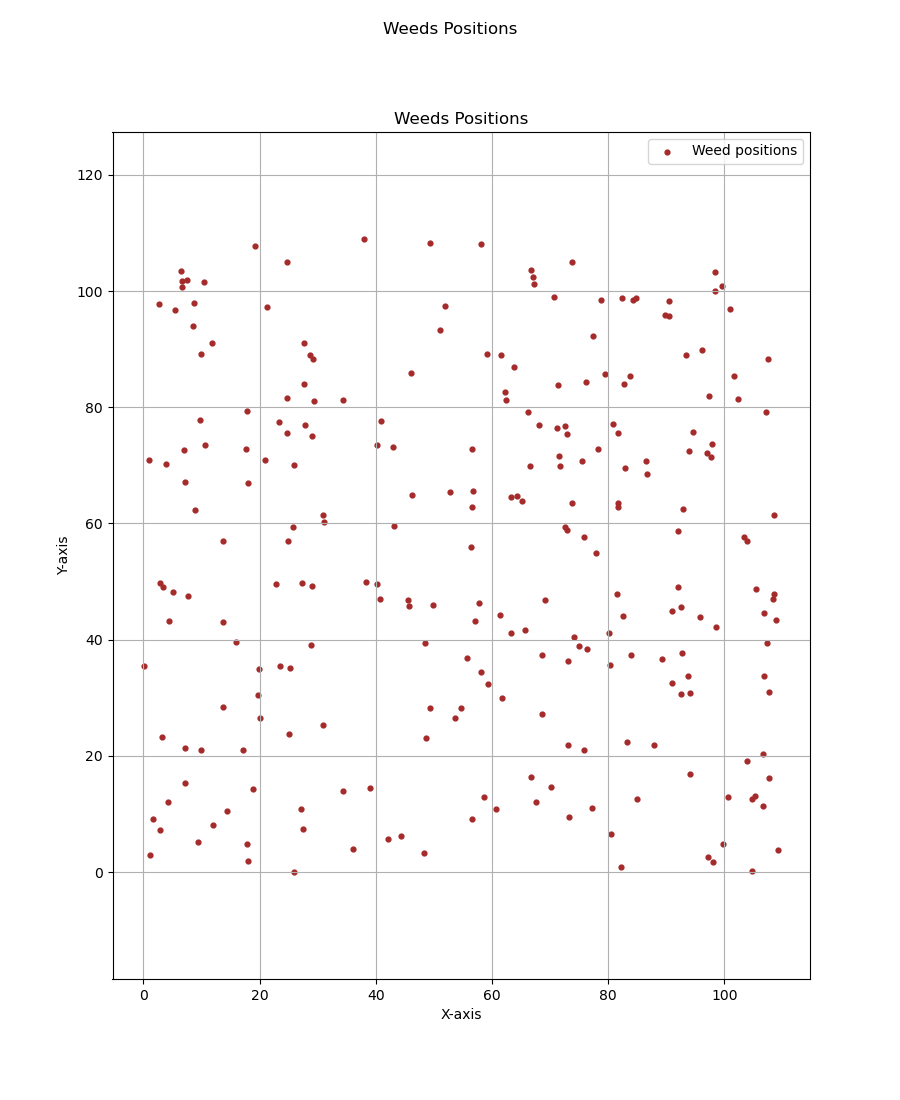
\includegraphics[height=36mm,width=0.24\textwidth]{Images/data/01.png}
        & 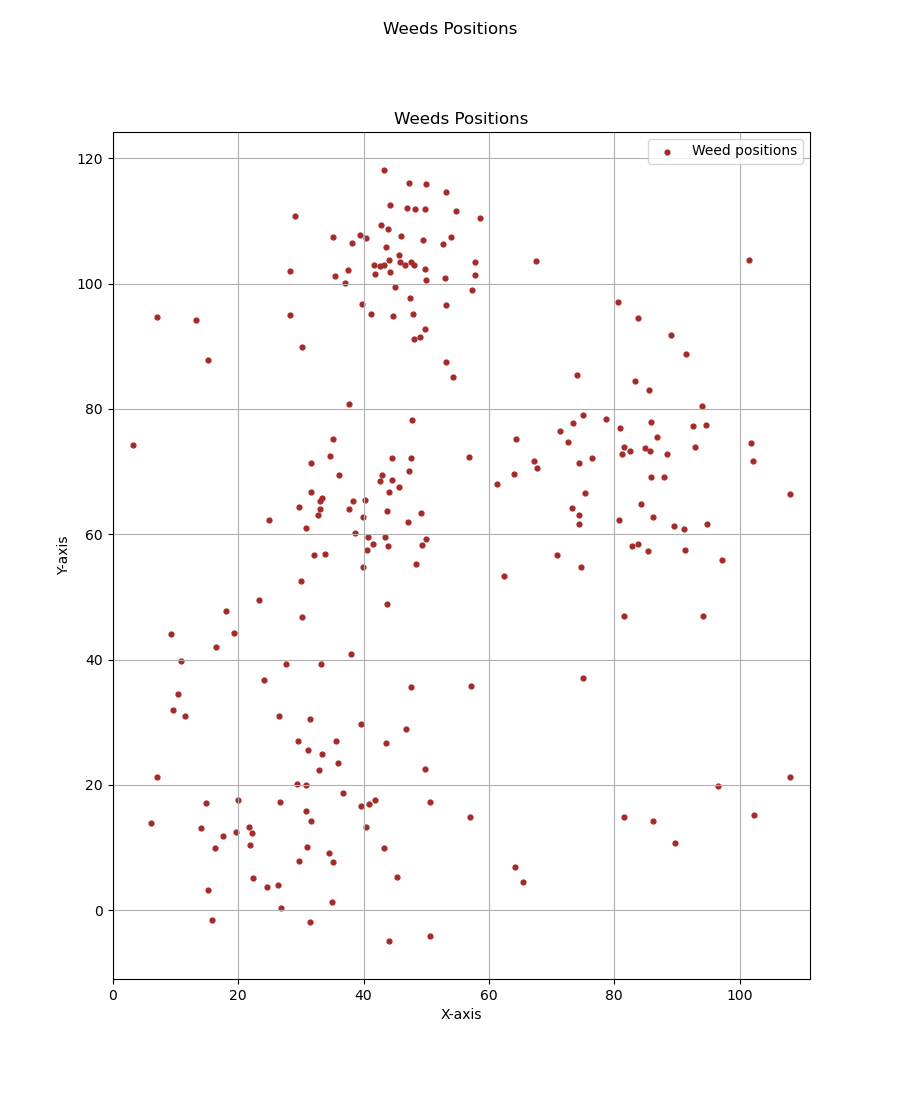
\includegraphics[height=36mm,width=0.24\textwidth]{Images/data/02.png}
        & 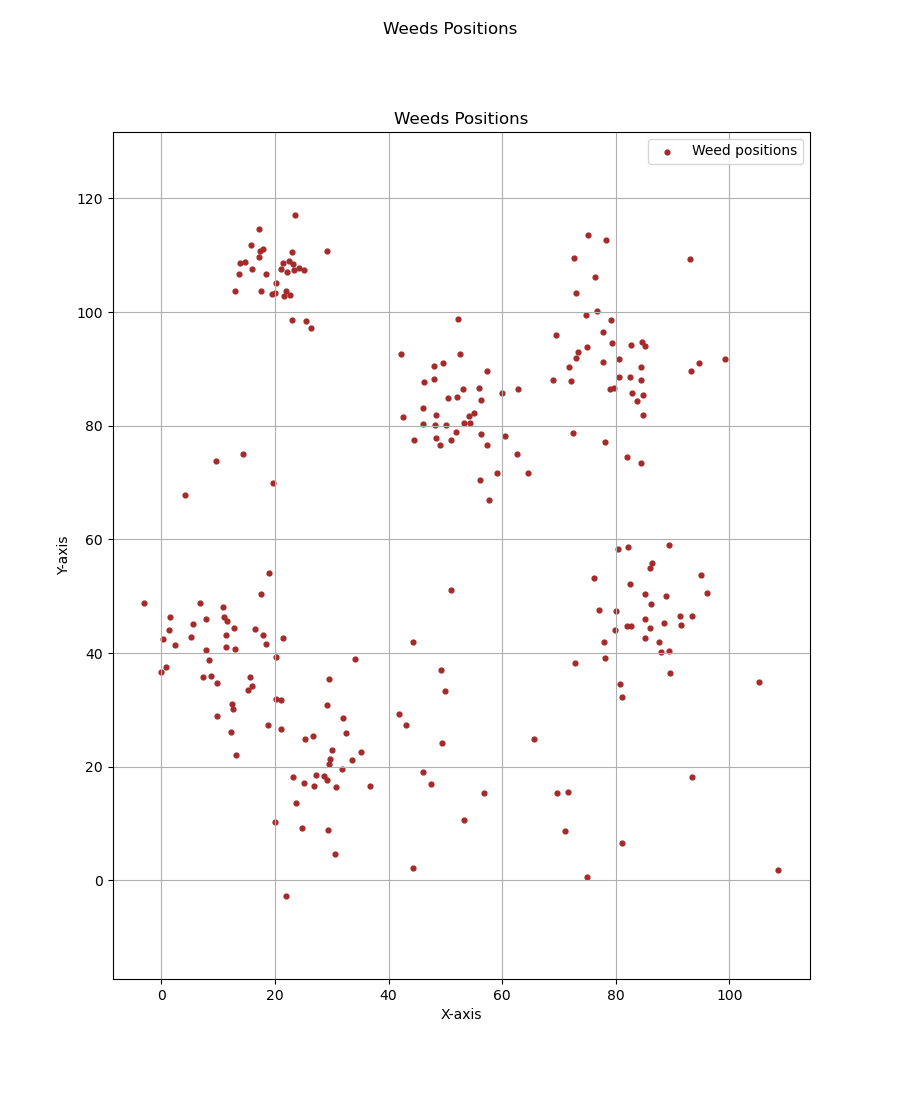
\includegraphics[height=36mm,width=0.24\textwidth]{Images/data/03.png}
         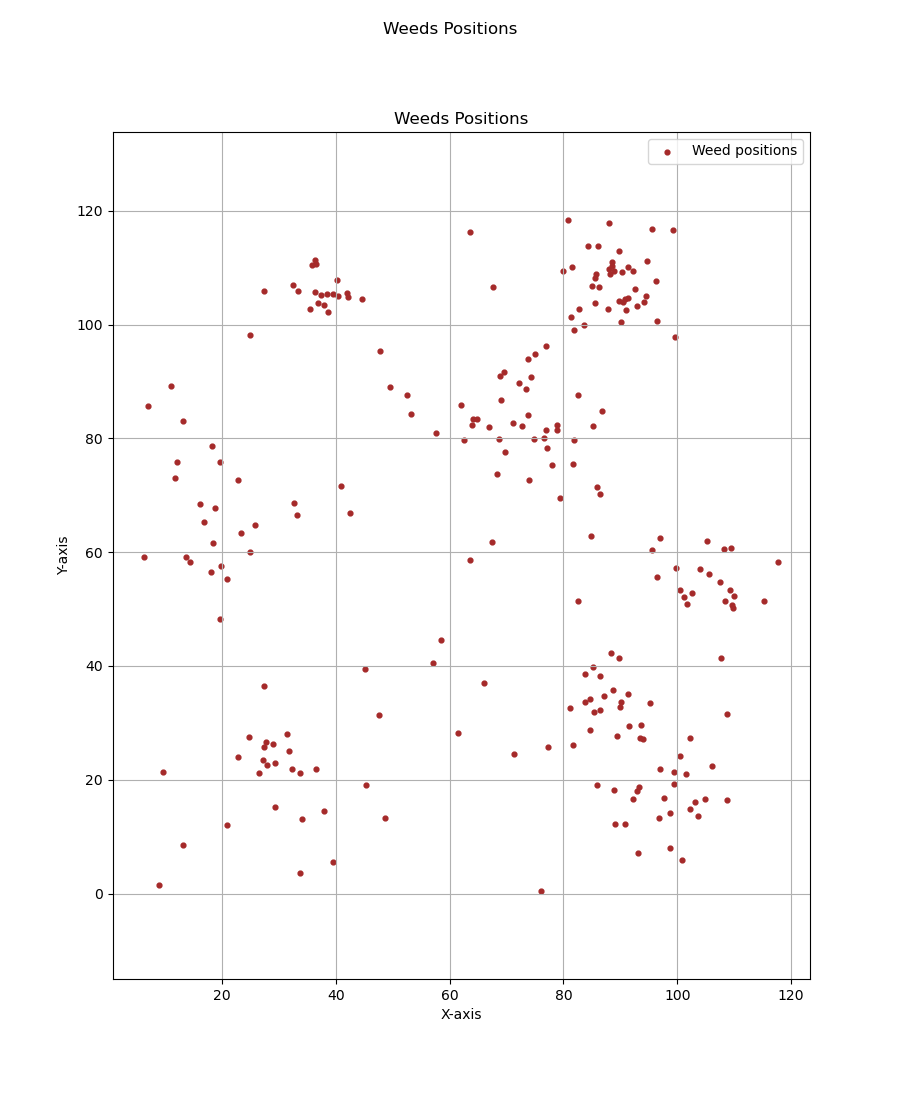
\includegraphics[height=36mm,width=0.24\textwidth]{Images/data/04.png}\\[-4pt]

        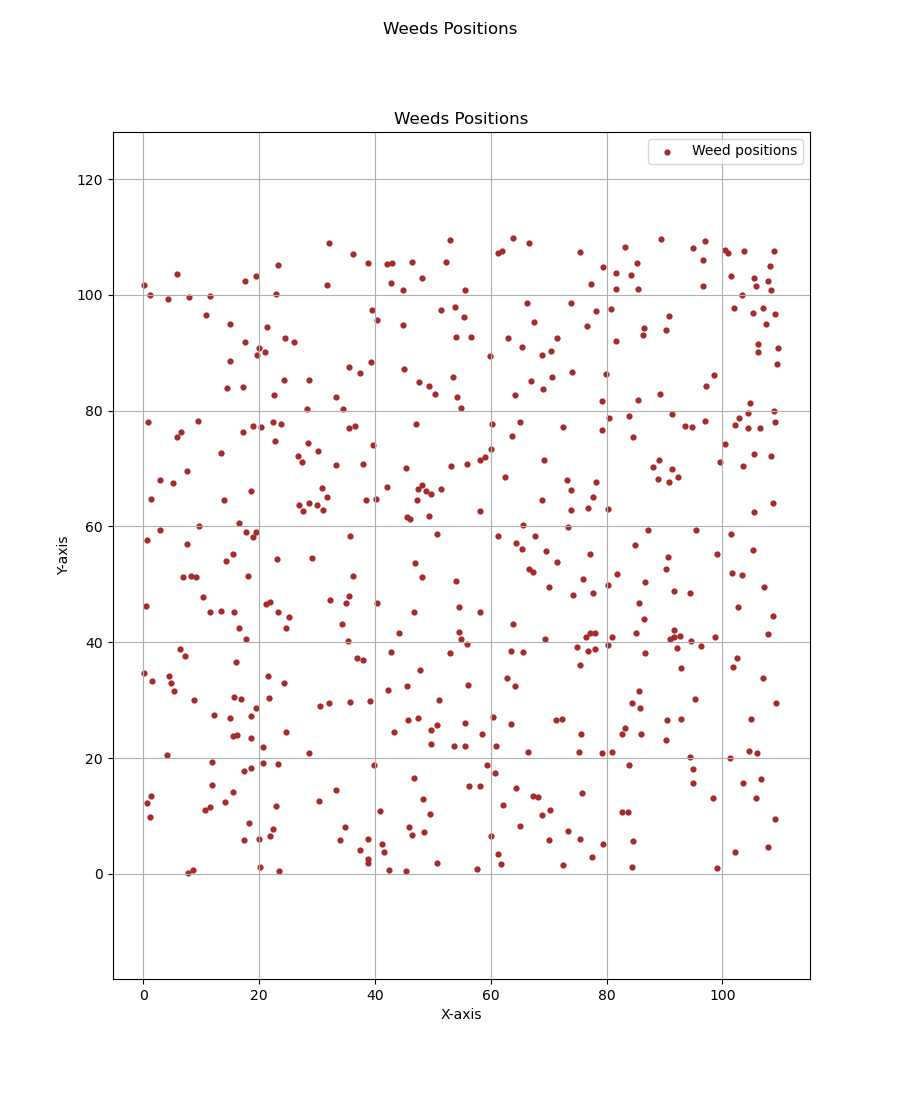
\includegraphics[height=36mm,width=0.24\textwidth]{Images/data/11.png}
        & 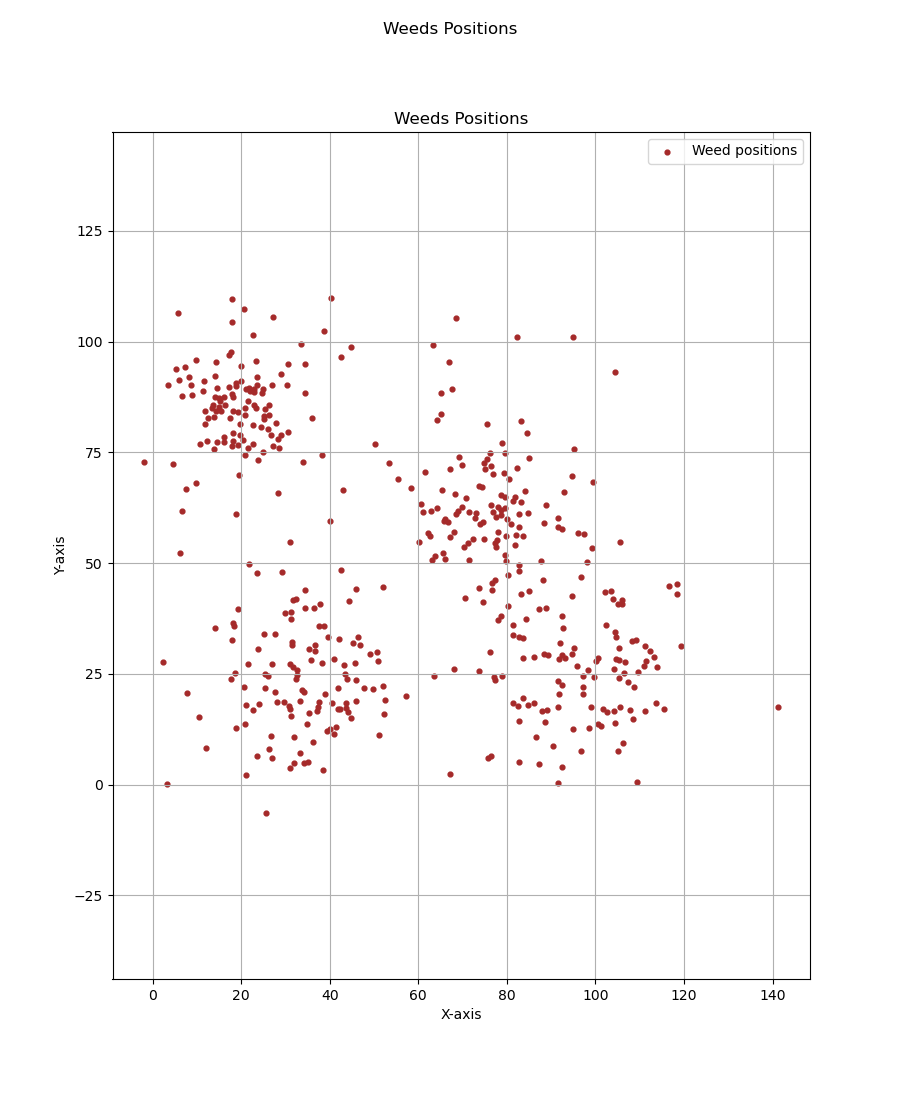
\includegraphics[height=36mm,width=0.24\textwidth]{Images/data/12.png}
        & 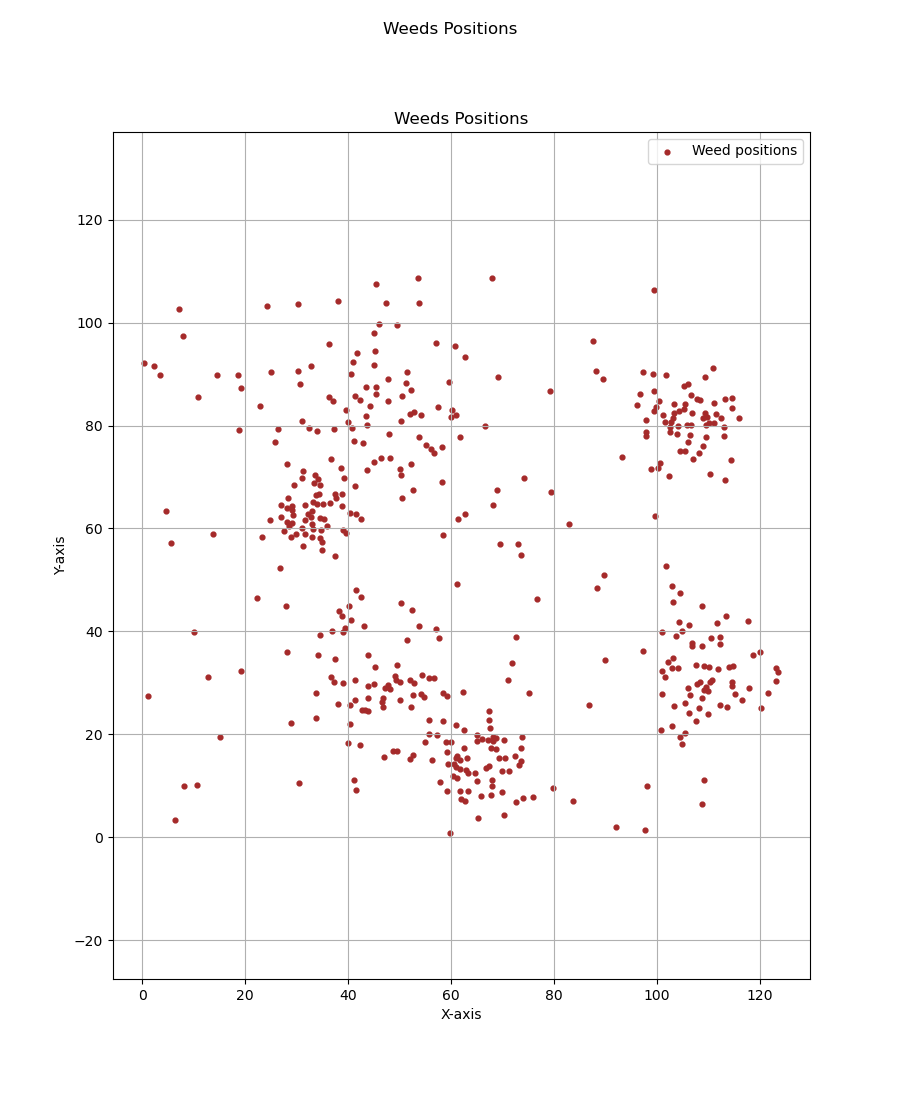
\includegraphics[height=36mm,width=0.24\textwidth]{Images/data/13.png}
        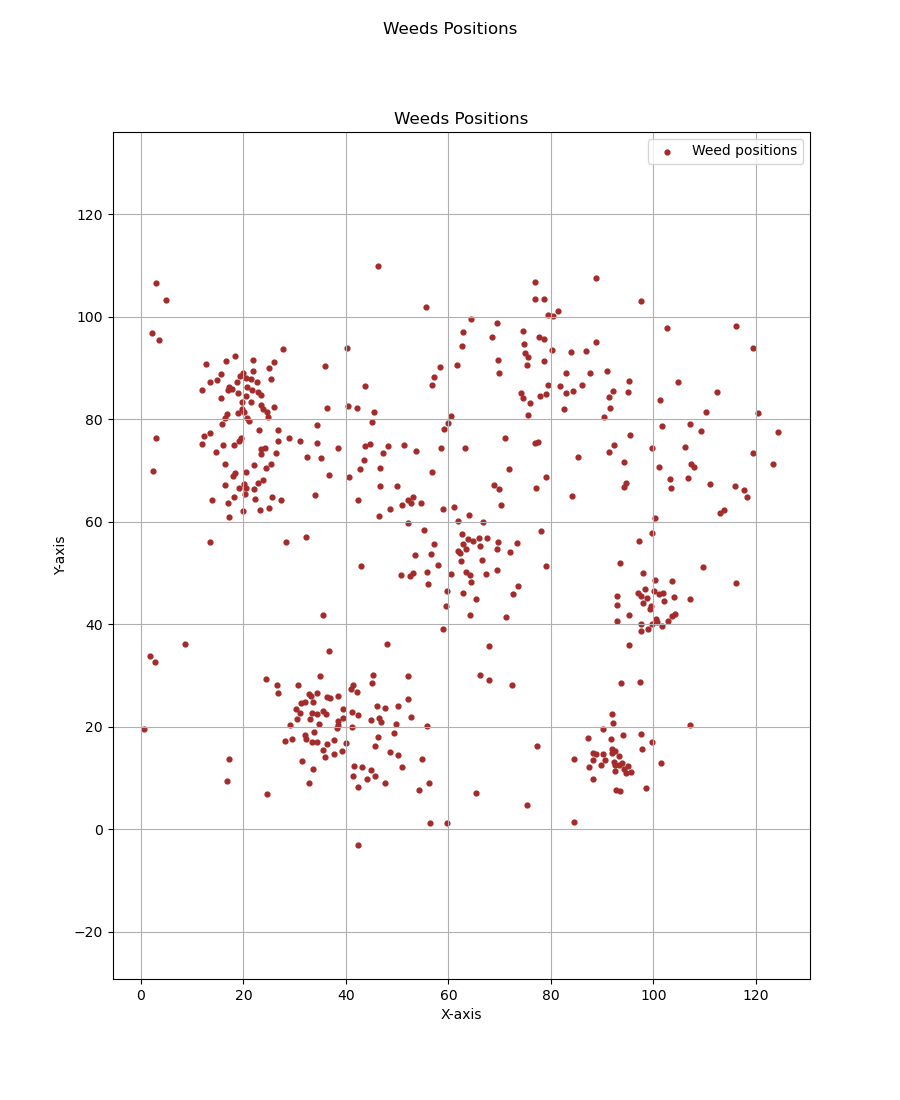
\includegraphics[height=36mm,width=0.24\textwidth]{Images/data/14.png}\\[-4pt]

        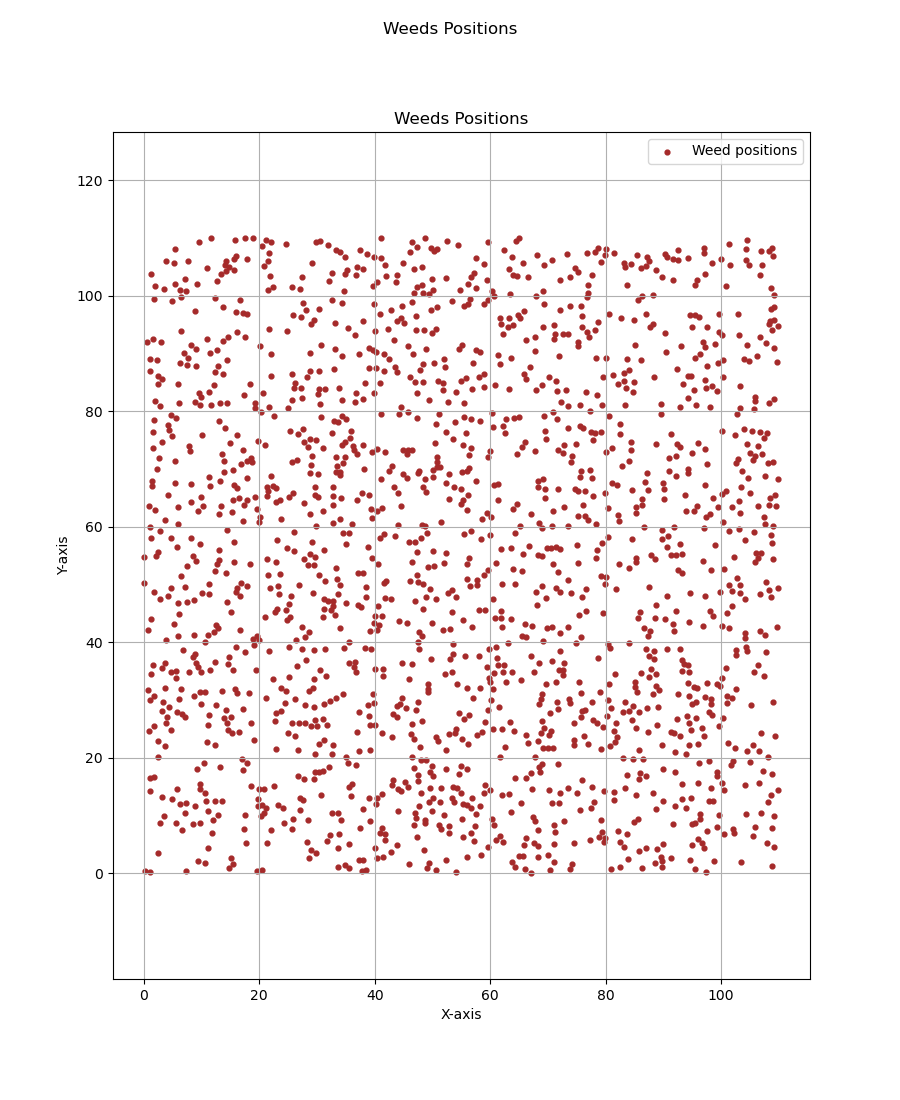
\includegraphics[height=36mm,width=0.24\textwidth]{Images/data/21.png}
        & 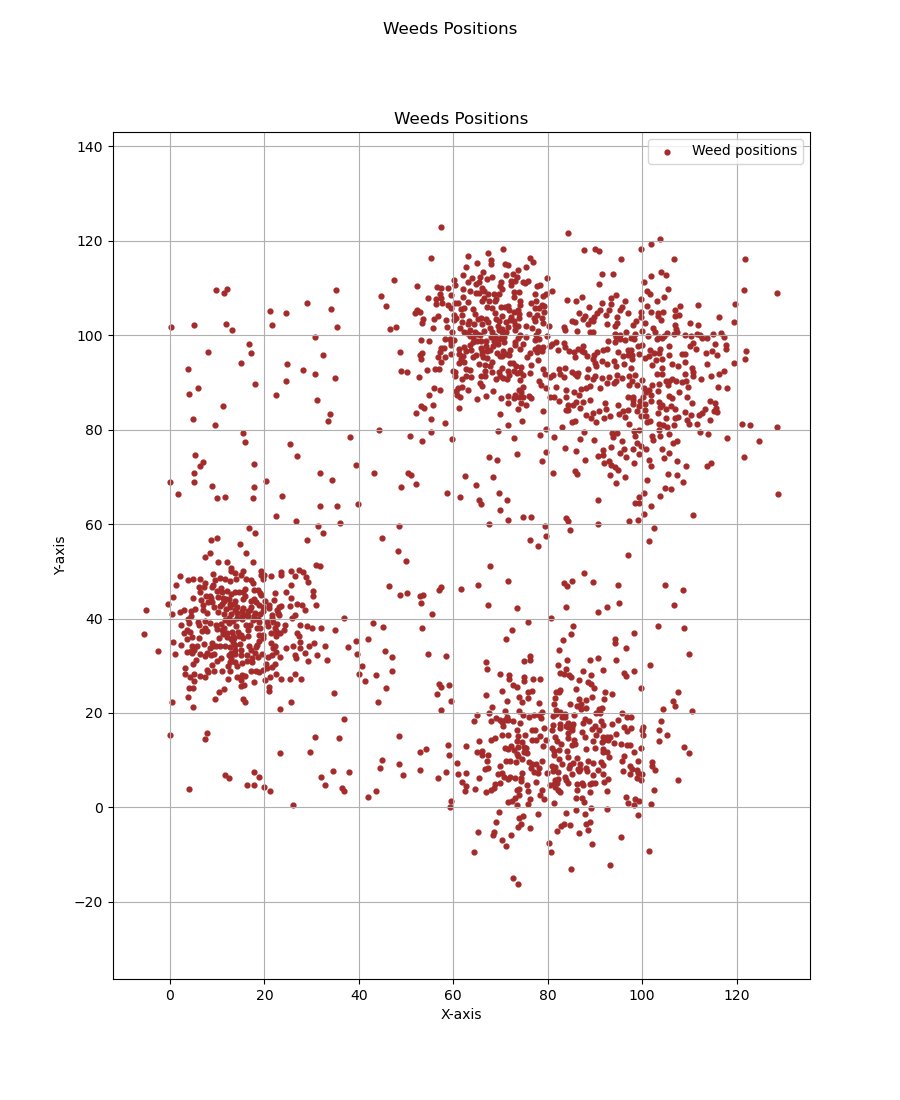
\includegraphics[height=36mm,width=0.24\textwidth]{Images/data/22.png}
        & 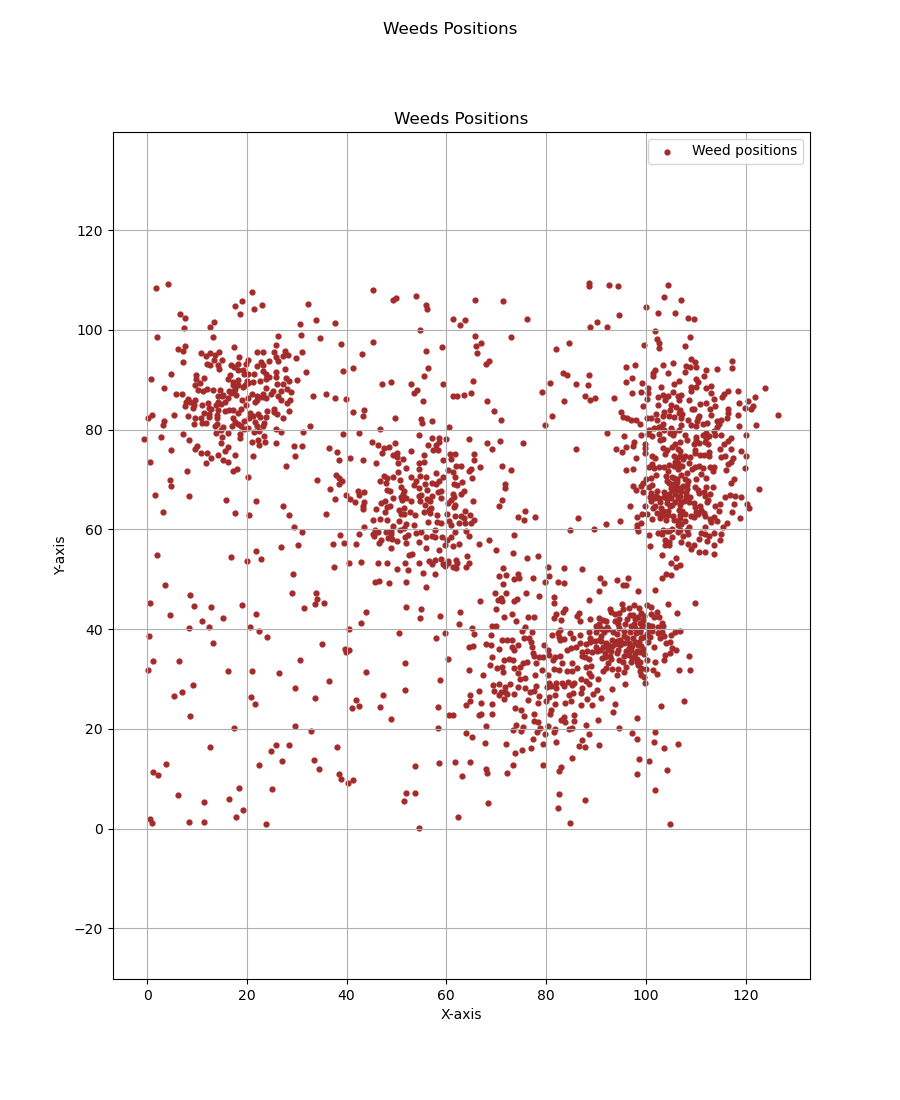
\includegraphics[height=36mm,width=0.24\textwidth]{Images/data/23.png}
         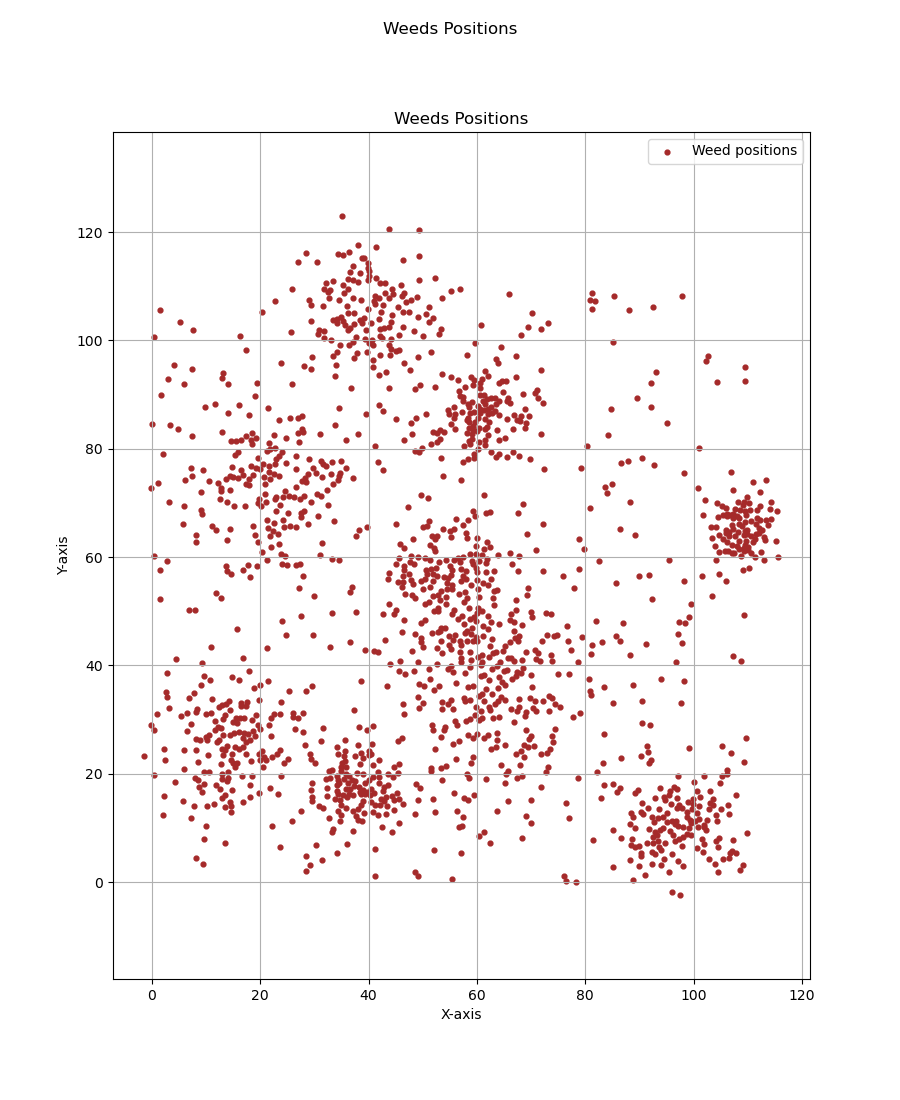
\includegraphics[height=36mm,width=0.24\textwidth]{Images/data/24.png}\\[-4pt]

         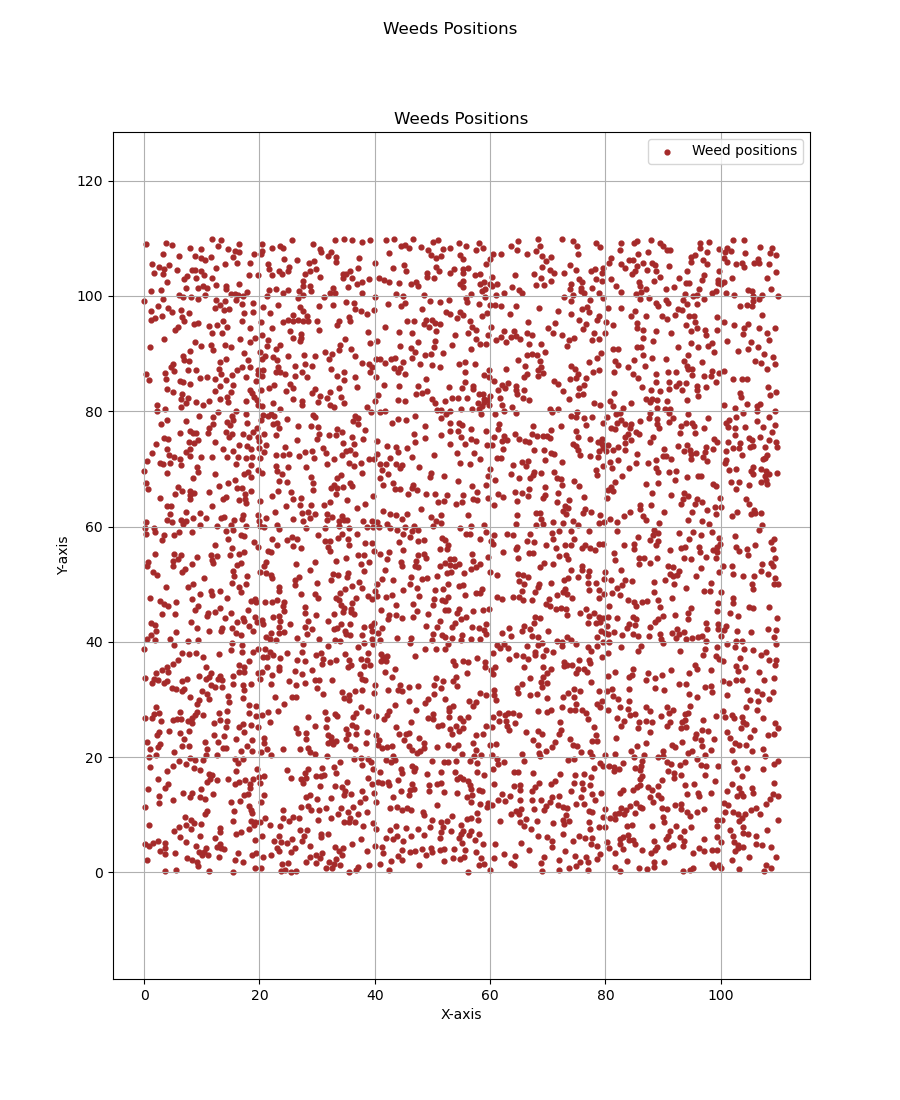
\includegraphics[height=36mm,width=0.24\textwidth]{Images/data/31.png}
        & 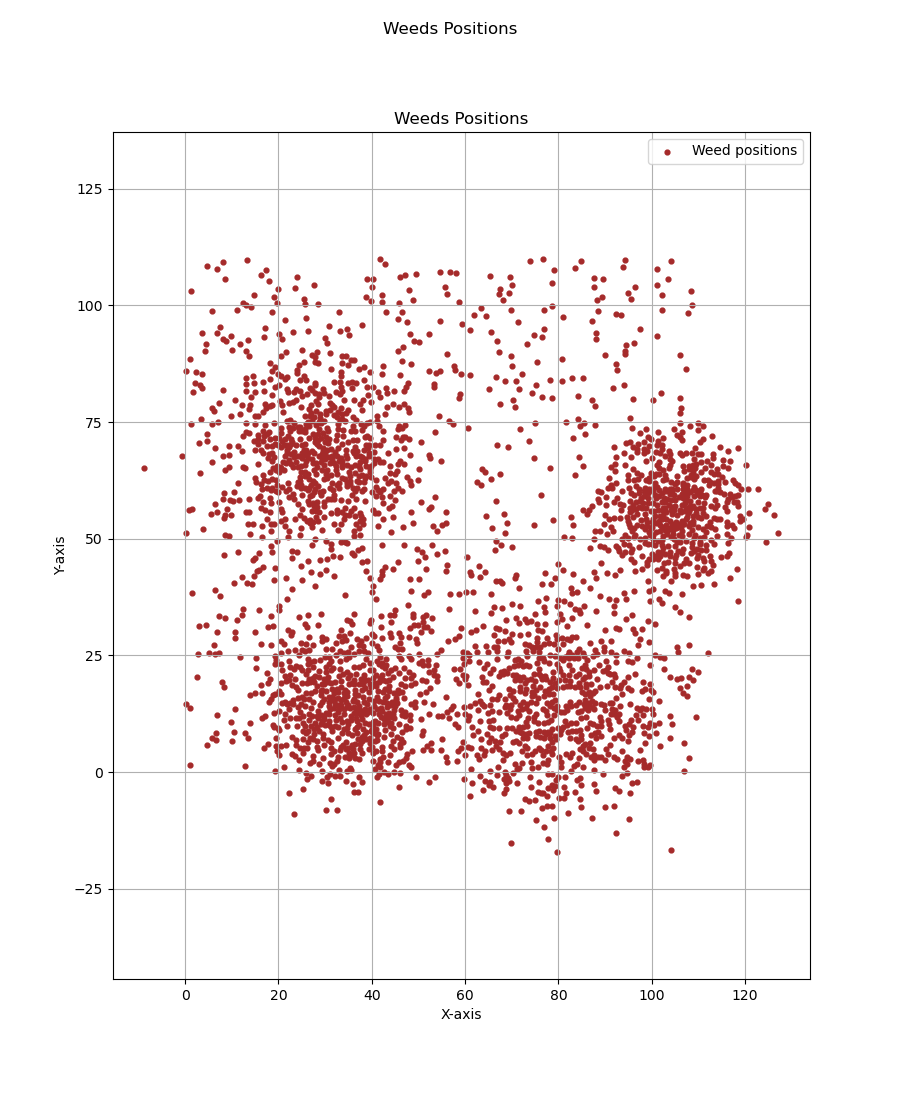
\includegraphics[height=36mm,width=0.24\textwidth]{Images/data/32.png}
        & 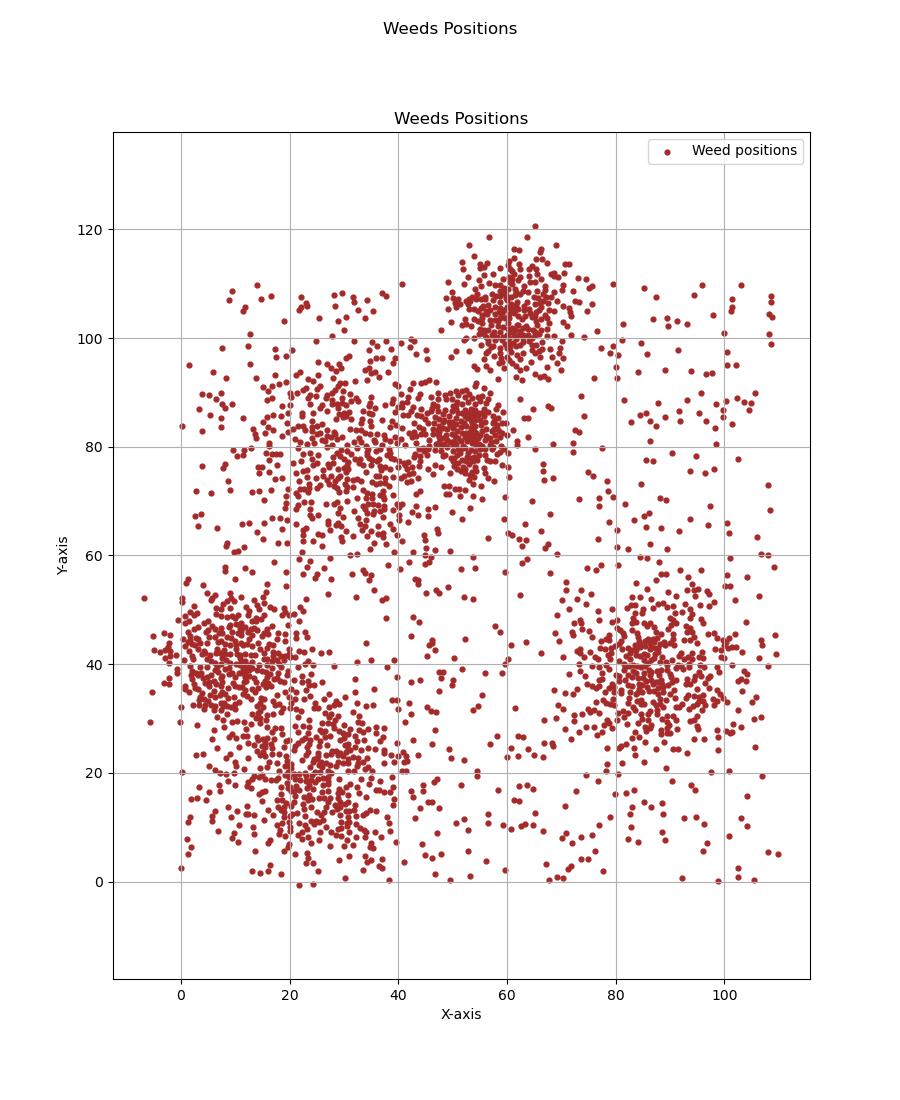
\includegraphics[height=36mm,width=0.24\textwidth]{Images/data/33.png}
         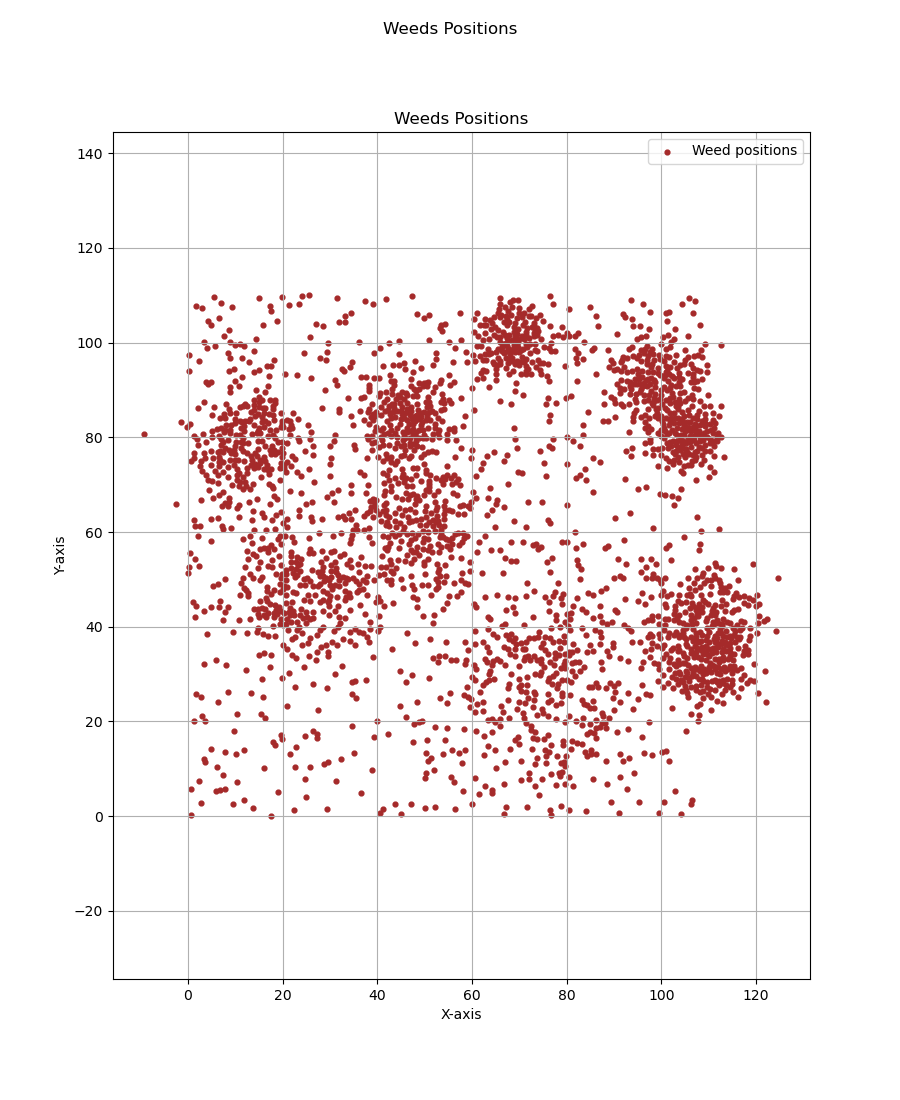
\includegraphics[height=36mm,width=0.24\textwidth]{Images/data/34.png}\\[-4pt]


        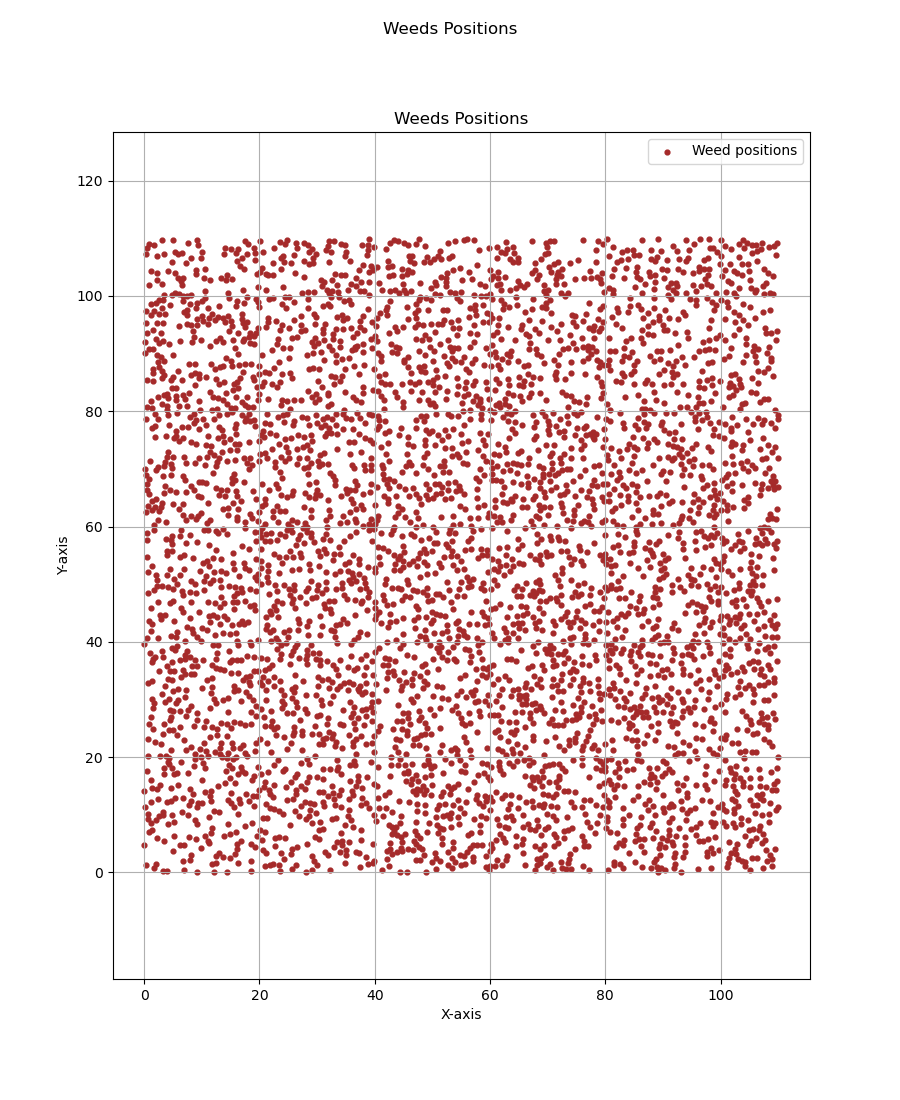
\includegraphics[height=36mm,width=0.24\textwidth]{Images/data/41.png}
        & 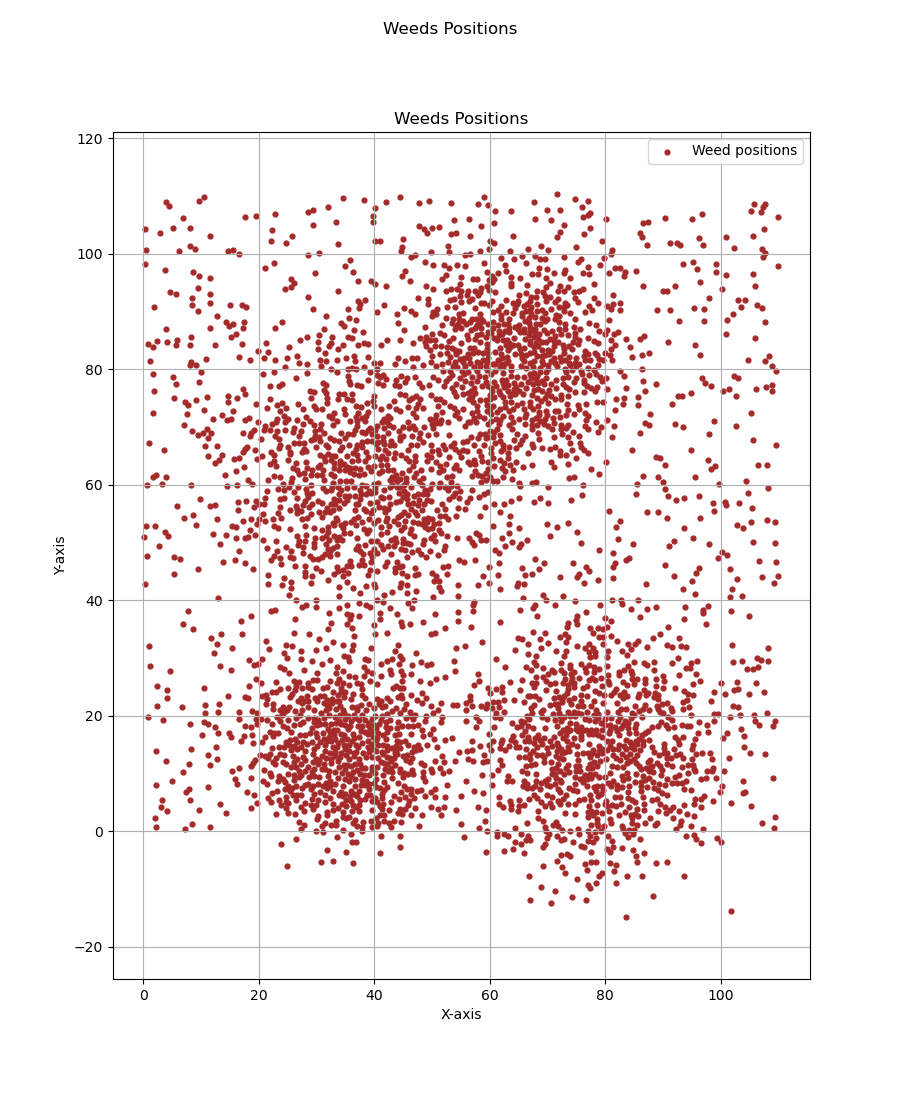
\includegraphics[height=36mm,width=0.24\textwidth]{Images/data/42.png}
        & 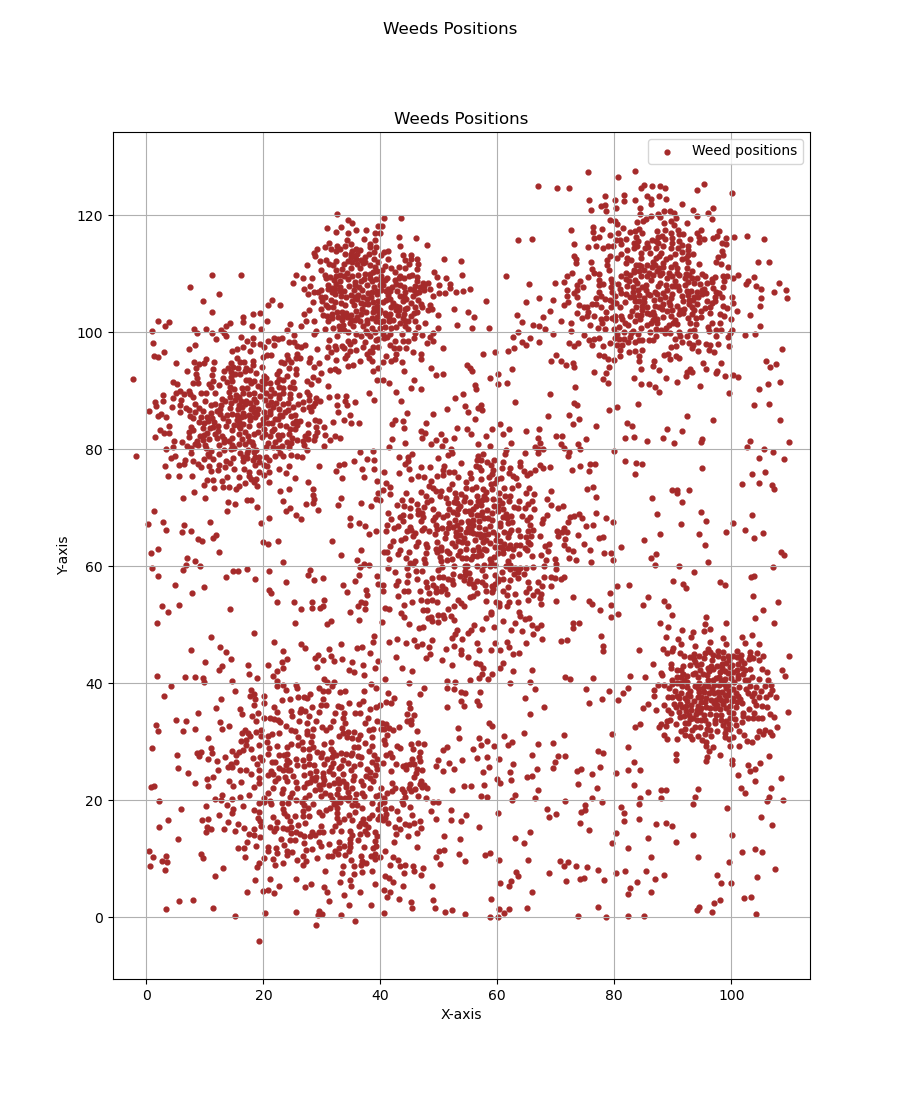
\includegraphics[height=36mm,width=0.24\textwidth]{Images/data/43.png}
        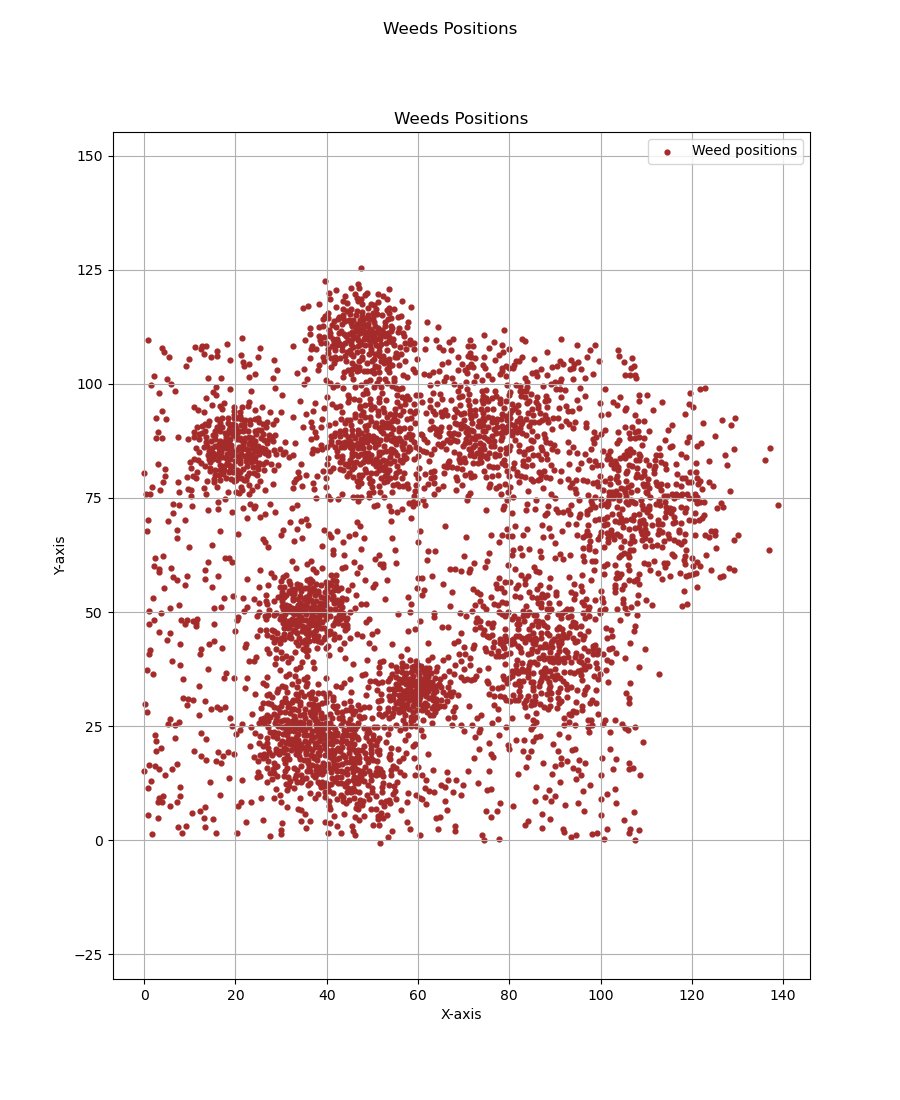
\includegraphics[height=36mm,width=0.24\textwidth]{Images/data/44.png}\\[-4pt]

        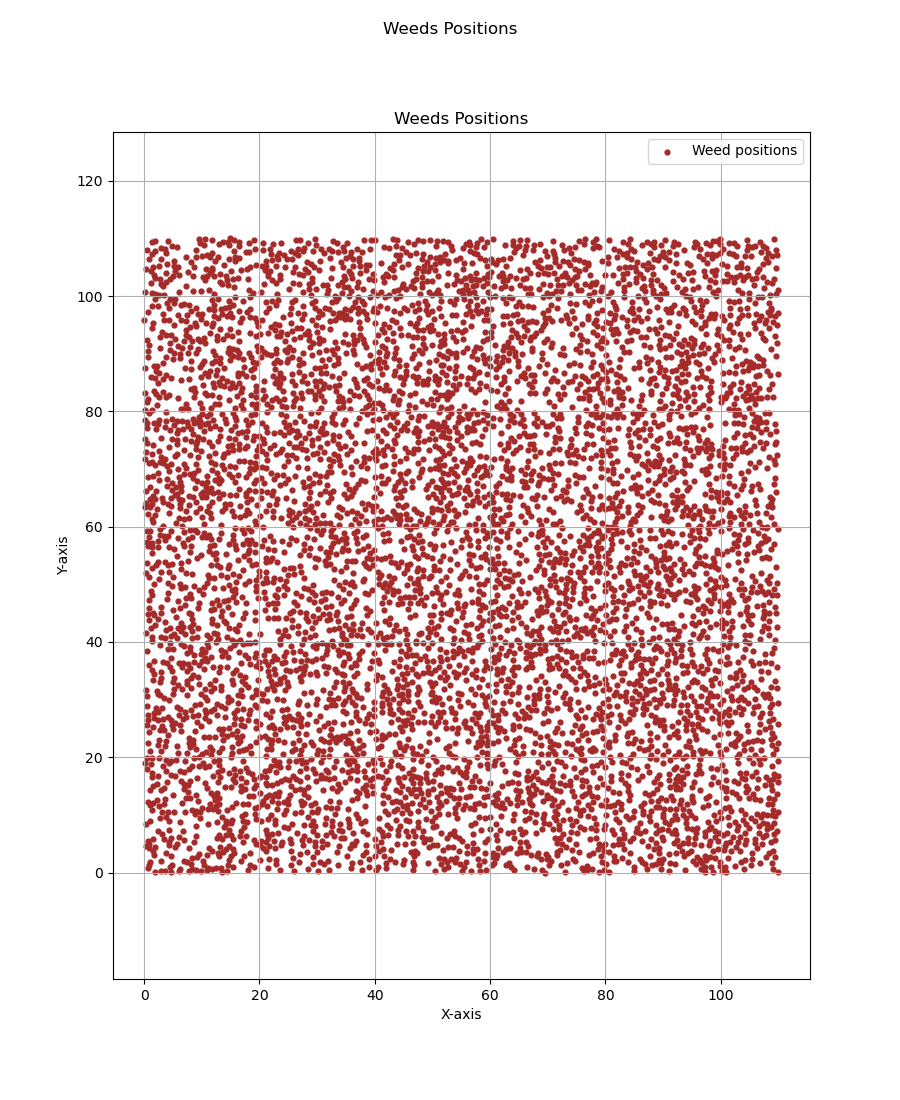
\includegraphics[height=36mm,width=0.24\textwidth]{Images/data/51.png}
        & 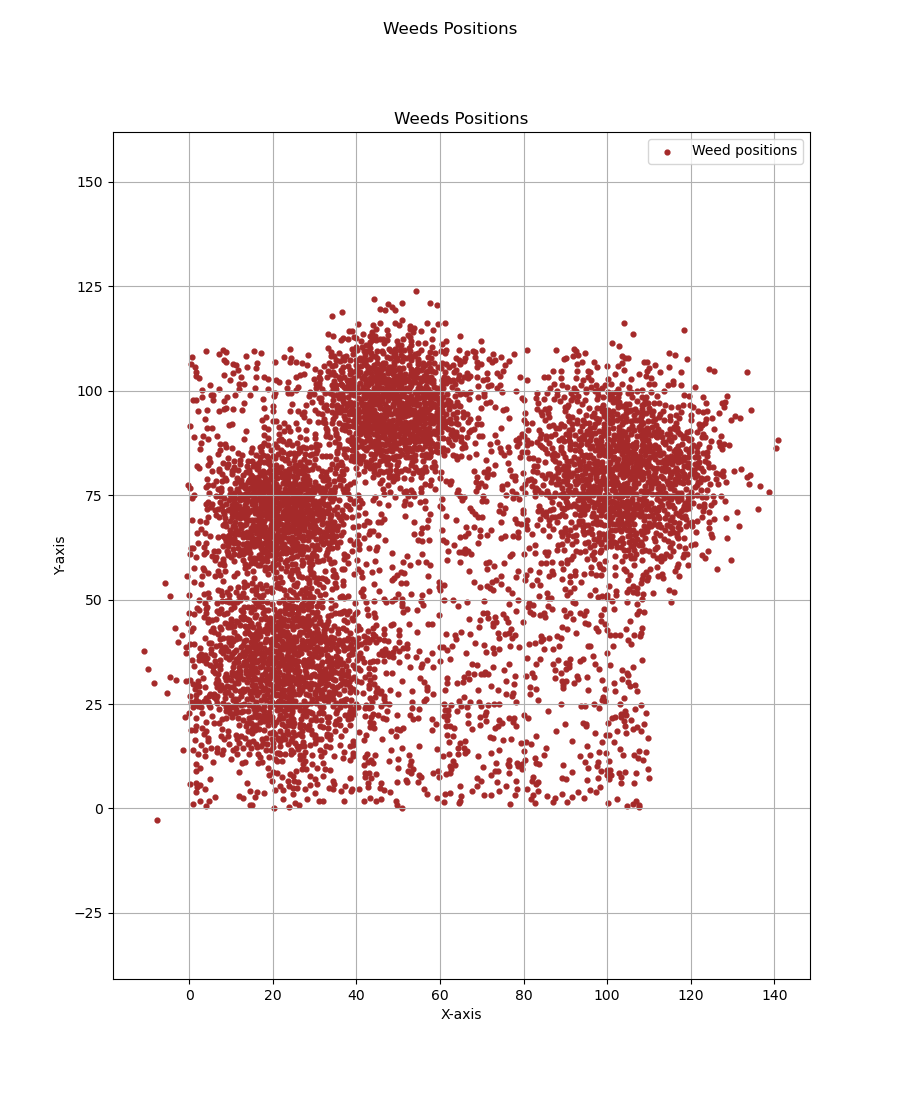
\includegraphics[height=36mm,width=0.24\textwidth]{Images/data/52.png}
        & 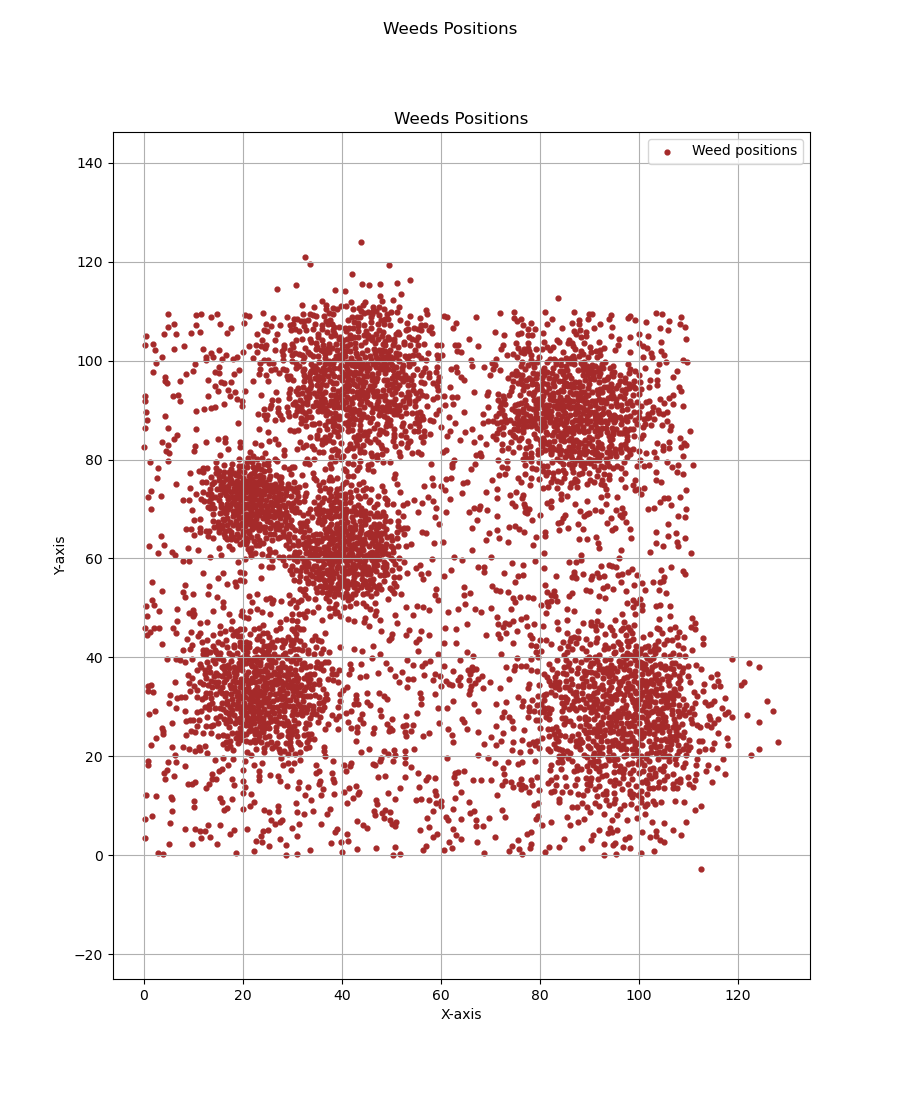
\includegraphics[height=36mm,width=0.24\textwidth]{Images/data/53.png}
        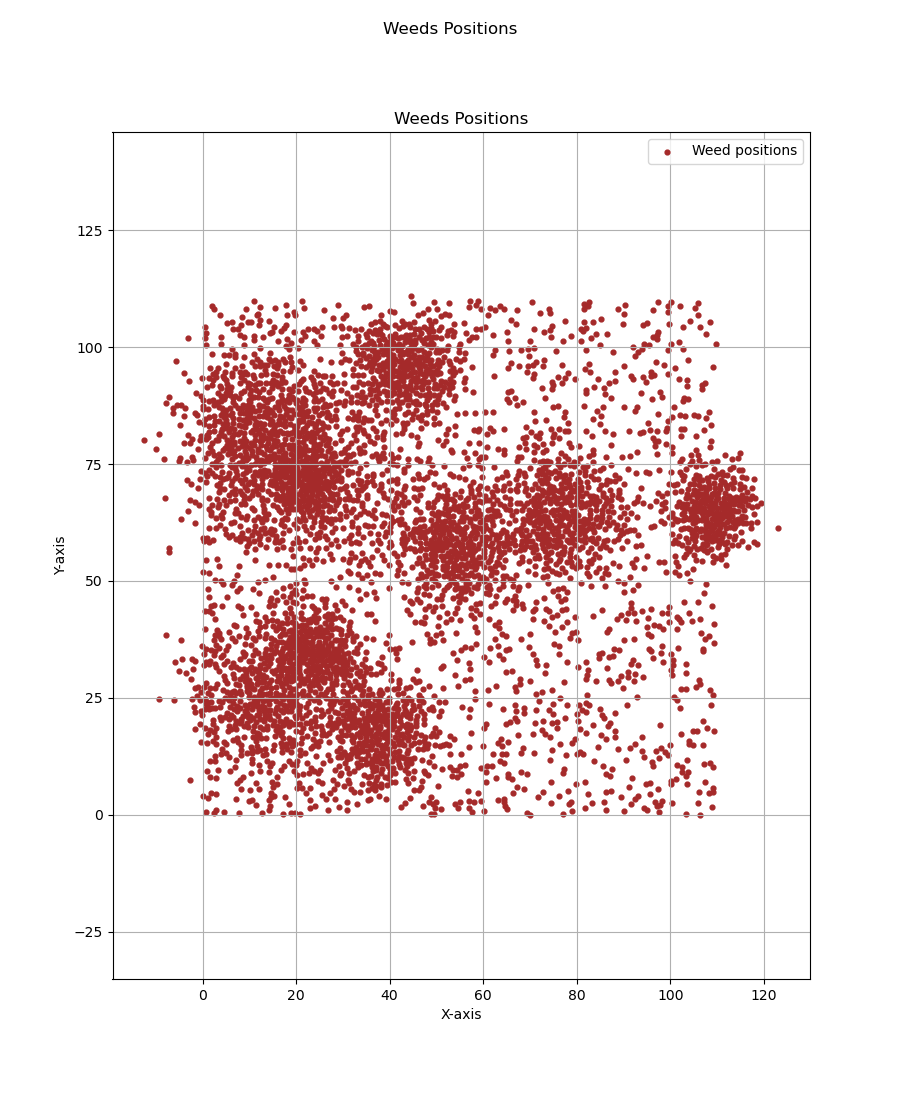
\includegraphics[height=36mm,width=0.24\textwidth]{Images/data/54.png}\\[-4pt]
        
    \end{tabular}
    \caption{Dataset.\label{fig:Dataset}}
\end{figure}


\section{Simulation Results and Analysis}

This section presents the detailed results and analysis of the simulation experiments conducted to evaluate the robustness of the proposed complete coverage path planning behavioral algorithm. The empirical findings are meticulously analyzed to provide insights into the algorithm's performance under diverse scenarios, enabling a comprehensive assessment of its efficiency and effectiveness. 

\vspace{3mm}  

\textbf{Experimental Consistency}
To ensure the validity of comparisons and isolate the effects of different datasets on the algorithm's performance, the initial position and orientation of the robot were kept constant throughout all experiments. Additionally, the parameters for both the robot and the algorithm were consistently maintained across all trials.


\vspace{3mm}  

\textbf{Robot Constraints and Algorithm Parameters: } 


The robot's constraints and operational parameters are set to realistic values to ensure the validity of the simulation results. The parameters' data can be visualized in (\autoref{tab:constraints_and_parameters_1}), offering a comprehensive overview of the robot's physical and operational characteristics.

% % % % % Table robot parameters 1
\begin{table}[H] 
    \centering
    \caption{Robot and algorithm Constraints and Parameters}
    \label{tab:constraints_and_parameters_1}
    \begin{tabular}{|c|c|}
    \hline
    \rowcolor[HTML]{FFCC67} 
    \textit{\textbf{Constraints and Parameters}}                                    & \textit{\textbf{Values}} \\ \hline
    \rowcolor[HTML]{BBF6F4} 
    \textit{Robot initial position}                                                 & {[}60.0, 1.0{]}          \\ \hline
    \rowcolor[HTML]{BBF6F4} 
    \textit{Robot initial orientation}                                              & 120                      \\ \hline
    \rowcolor[HTML]{BBF6F4} 
    \textit{Search angle of the vision cone}                                        & ±11                      \\ \hline
    \rowcolor[HTML]{BBF6F4} 
    \textit{Minimum search radius of the vision cone.}                              & 1.25                     \\ \hline
    \rowcolor[HTML]{BBF6F4} 
    \textit{Maximum search radius of the vision cone.}                              & 100                      \\ \hline
    \rowcolor[HTML]{BBF6F4} 
    \textit{Minimum turning radius allowed for the robot.}                          & 2.0                      \\ \hline
    \rowcolor[HTML]{BBF6F4} 
    \textit{robot velocity on curved paths.}                                        & 0.4                      \\ \hline
    \rowcolor[HTML]{BBF6F4} 
    \textit{robot velocity on straight paths.}                                      & 0.8                      \\ \hline
    \rowcolor[HTML]{BBF6F4} 
    \textit{Distance used to compute field time taken on curved paths.}             & 7.85                     \\ \hline
    \rowcolor[HTML]{BBF6F4} 
    \textit{Number of points to consider in the vision cone.}                       & 5                        \\ \hline
    \rowcolor[HTML]{BEF7F5} 
    \textit{Minimum distance between intermediate points, and start and end point.} & 2.7                      \\ \hline
    \rowcolor[HTML]{BEF7F5} 
    \textit{Minimum distance between intermediate points.}                          & 2                        \\ \hline
    \rowcolor[HTML]{BEF7F5} 
    \textit{Maximum distance of the point form the path.}                           & 0.6                      \\ \hline
    \end{tabular}
    \end{table}



\vspace{3mm}   







The algorithm parameters are also meticulously defined to ensure consistent performance across all experiments. These parameters are set based on the robot's physical constraints and operational requirements, ensuring that the algorithm operates within realistic boundaries.

\vspace{3mm}

The algorithm was designed to initially compute the global coverage path using straight lines. Subsequently, Dubins paths are generated for each line segment to ensure the shortest feasible path between each pair of points, optimizing the overall path length. The (\autoref{fig:straight_path}) illustrate the straight paths generated by the algorithm for different datasets.

% Straight_path
\begin{figure}[p]
    \centering
    \begin{tabular}{ccc}
         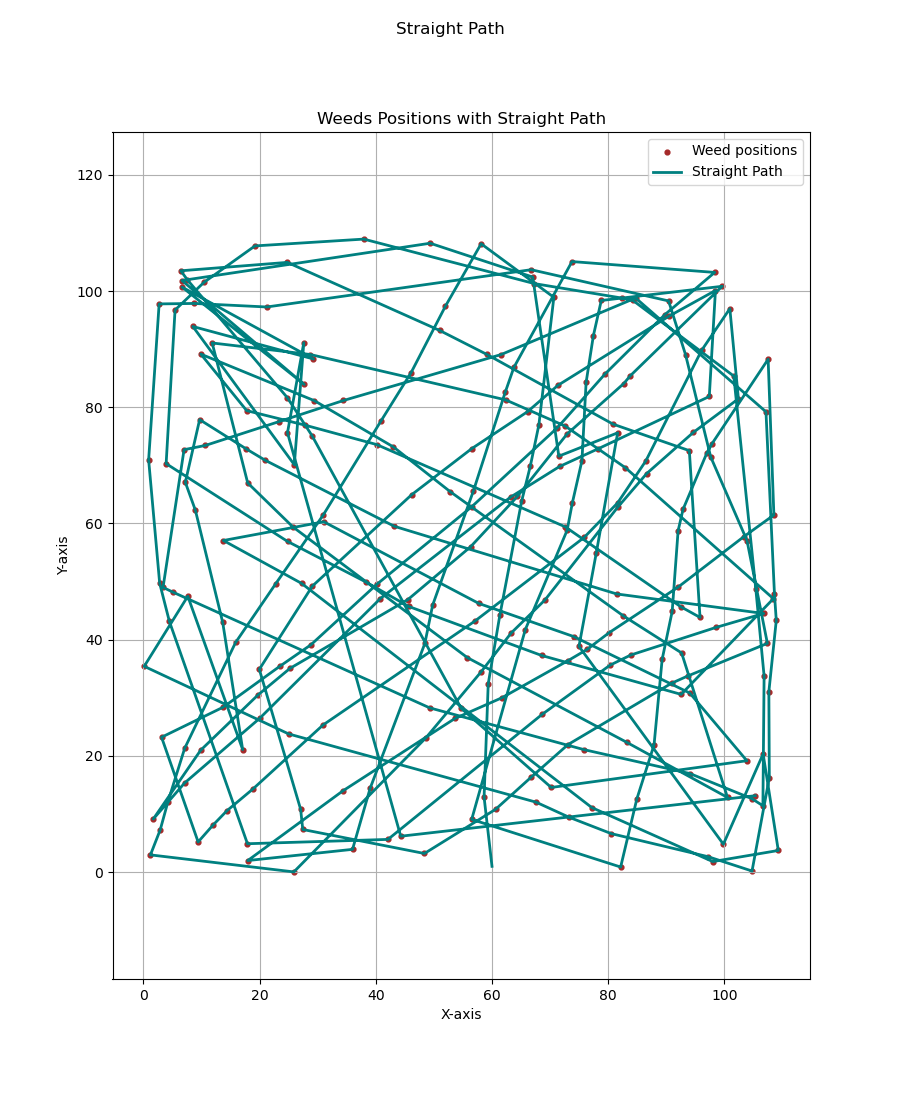
\includegraphics[height=36mm,width=0.24\textwidth]{Images/simulation_no_obs/straight_paths/01.png}
        & 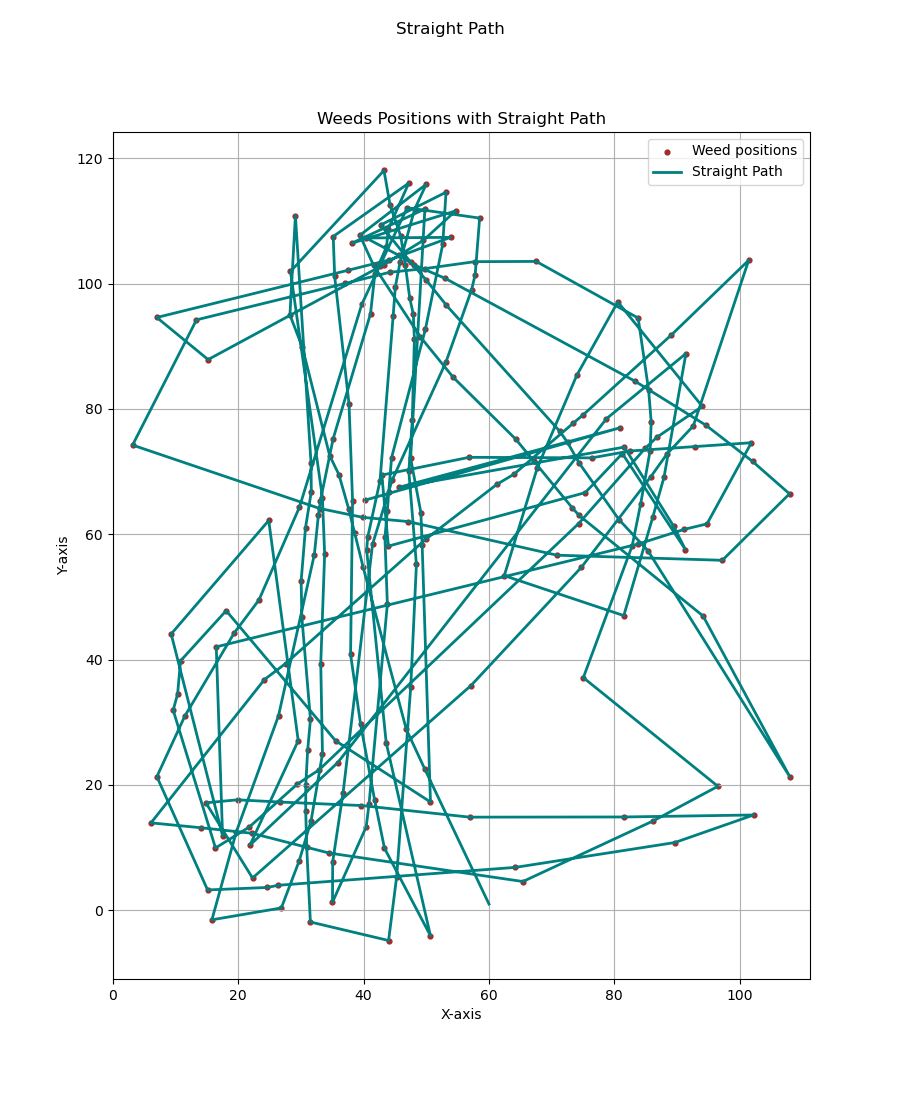
\includegraphics[height=36mm,width=0.24\textwidth]{Images/simulation_no_obs/straight_paths/02.png}
        & 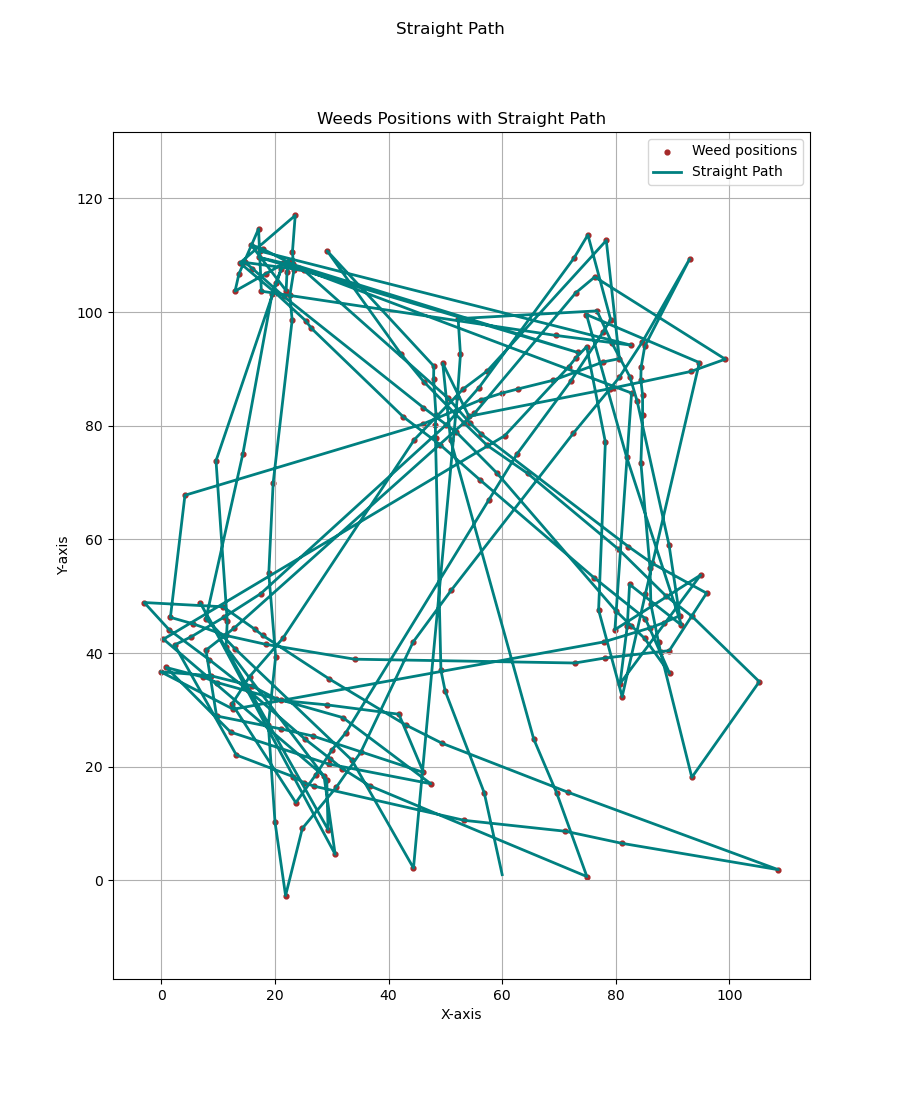
\includegraphics[height=36mm,width=0.24\textwidth]{Images/simulation_no_obs/straight_paths/03.png}
         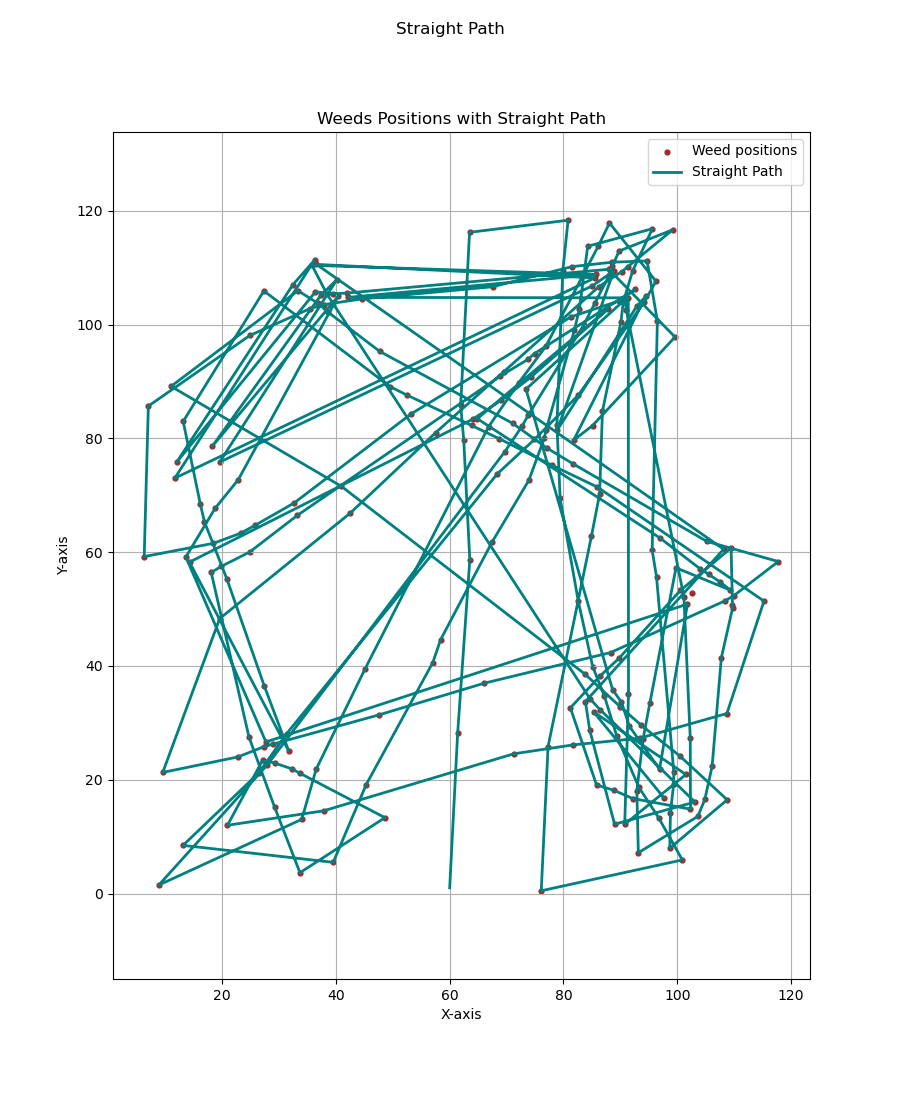
\includegraphics[height=36mm,width=0.24\textwidth]{Images/simulation_no_obs/straight_paths/04.png}\\[-4pt]

        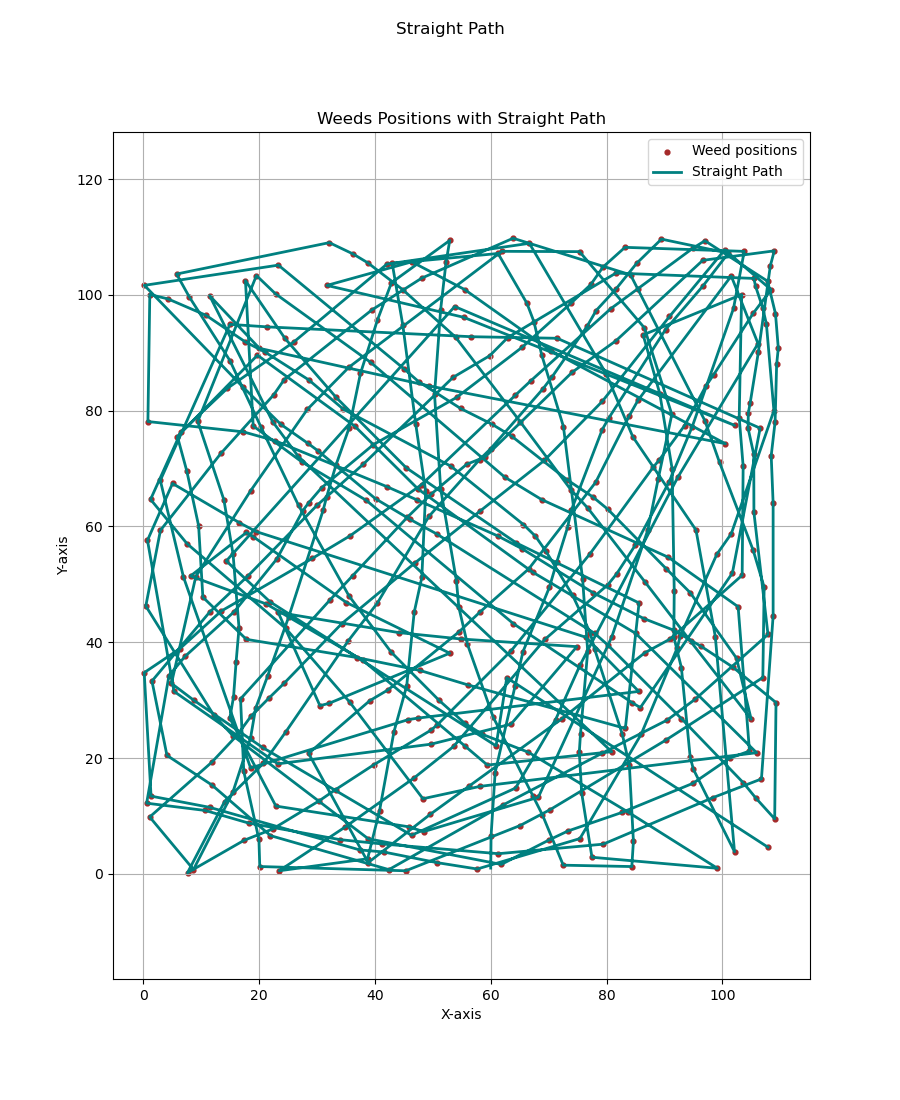
\includegraphics[height=36mm,width=0.24\textwidth]{Images/simulation_no_obs/straight_paths/11.png}
        & 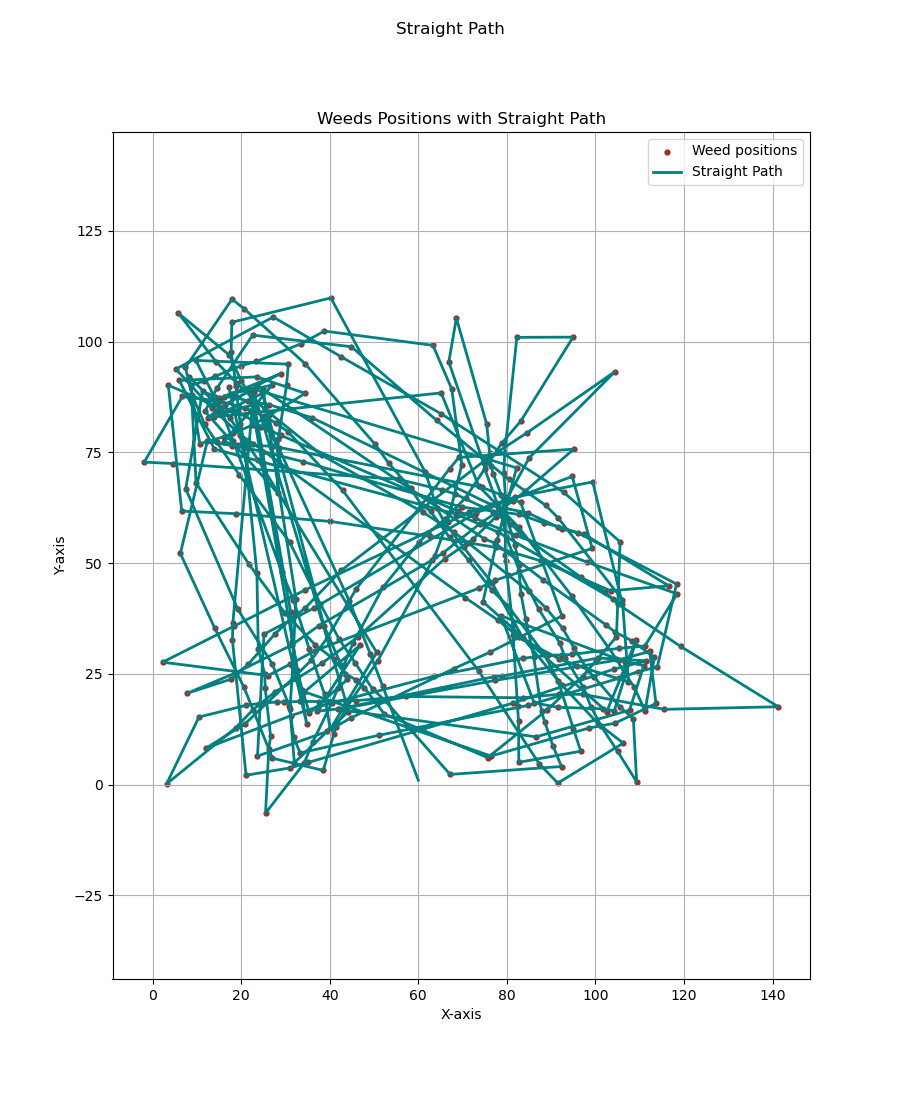
\includegraphics[height=36mm,width=0.24\textwidth]{Images/simulation_no_obs/straight_paths/12.png}
        & 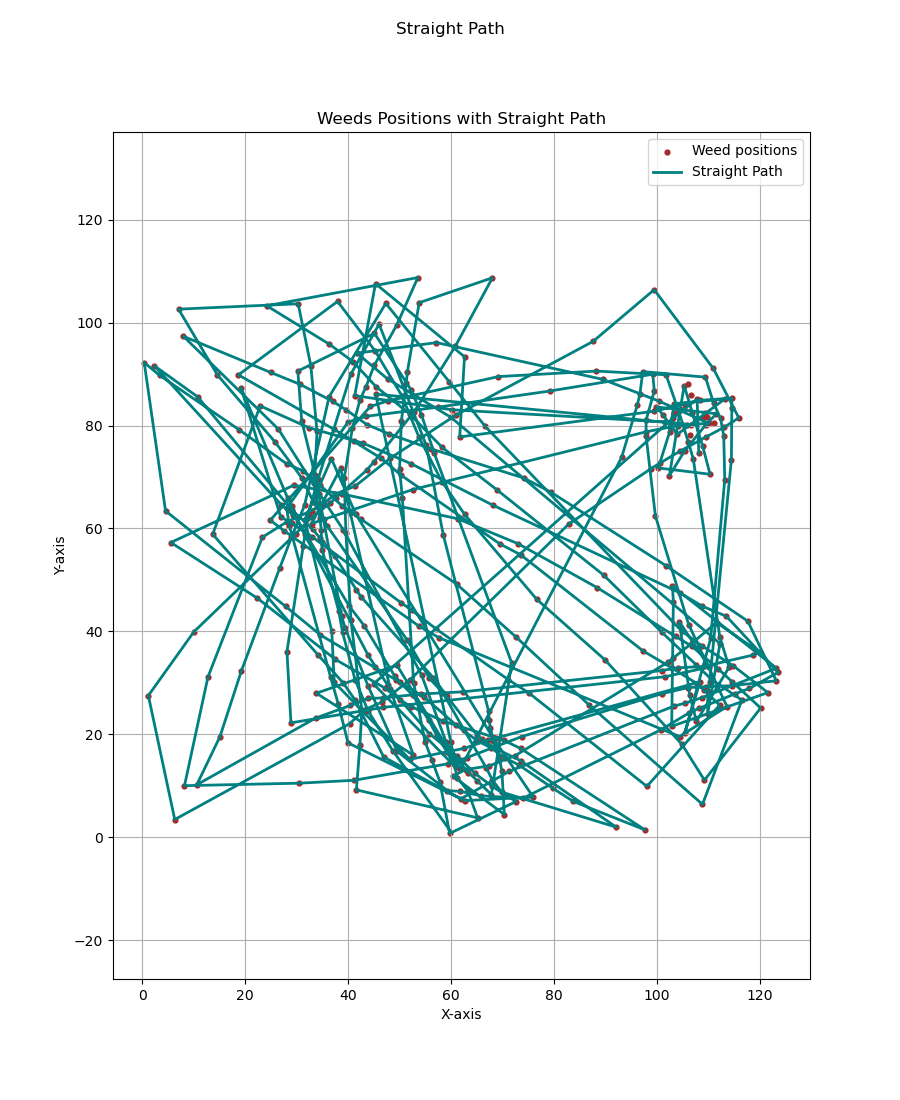
\includegraphics[height=36mm,width=0.24\textwidth]{Images/simulation_no_obs/straight_paths/13.png}
        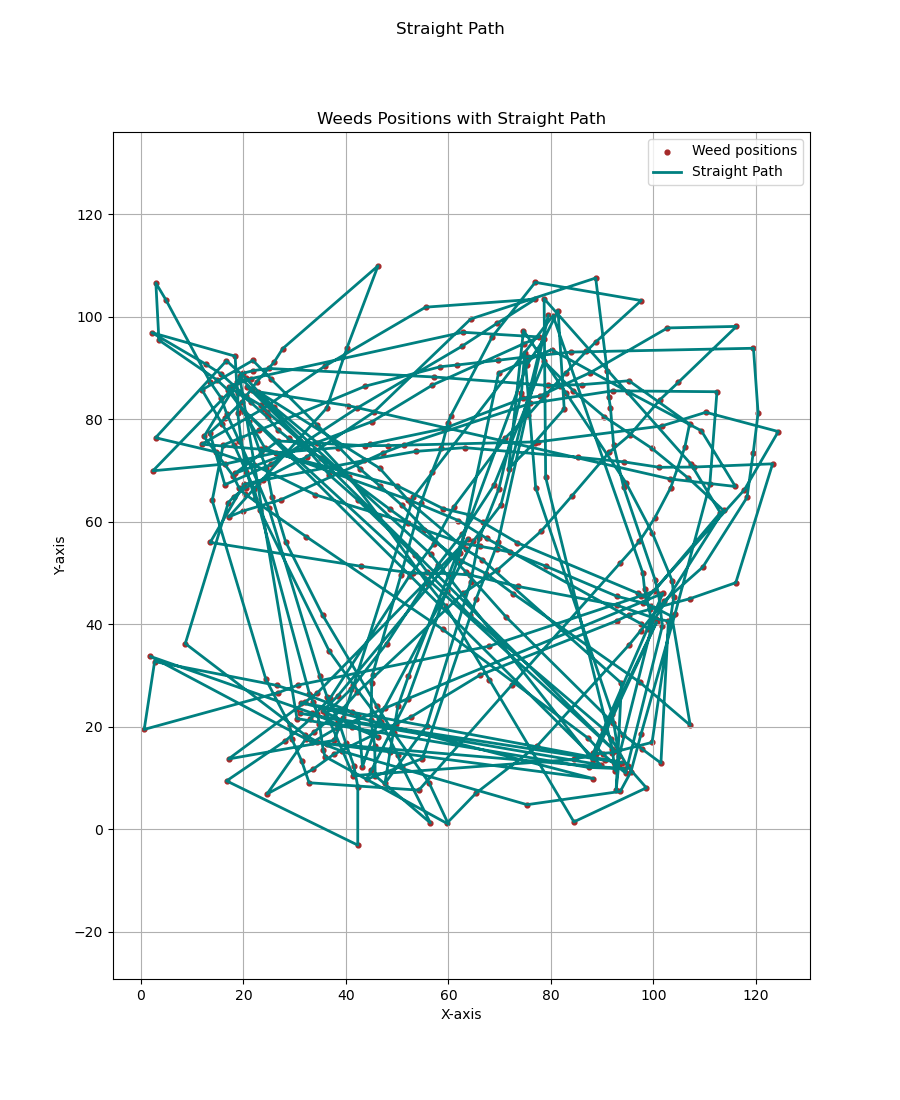
\includegraphics[height=36mm,width=0.24\textwidth]{Images/simulation_no_obs/straight_paths/14.png}\\[-4pt]

        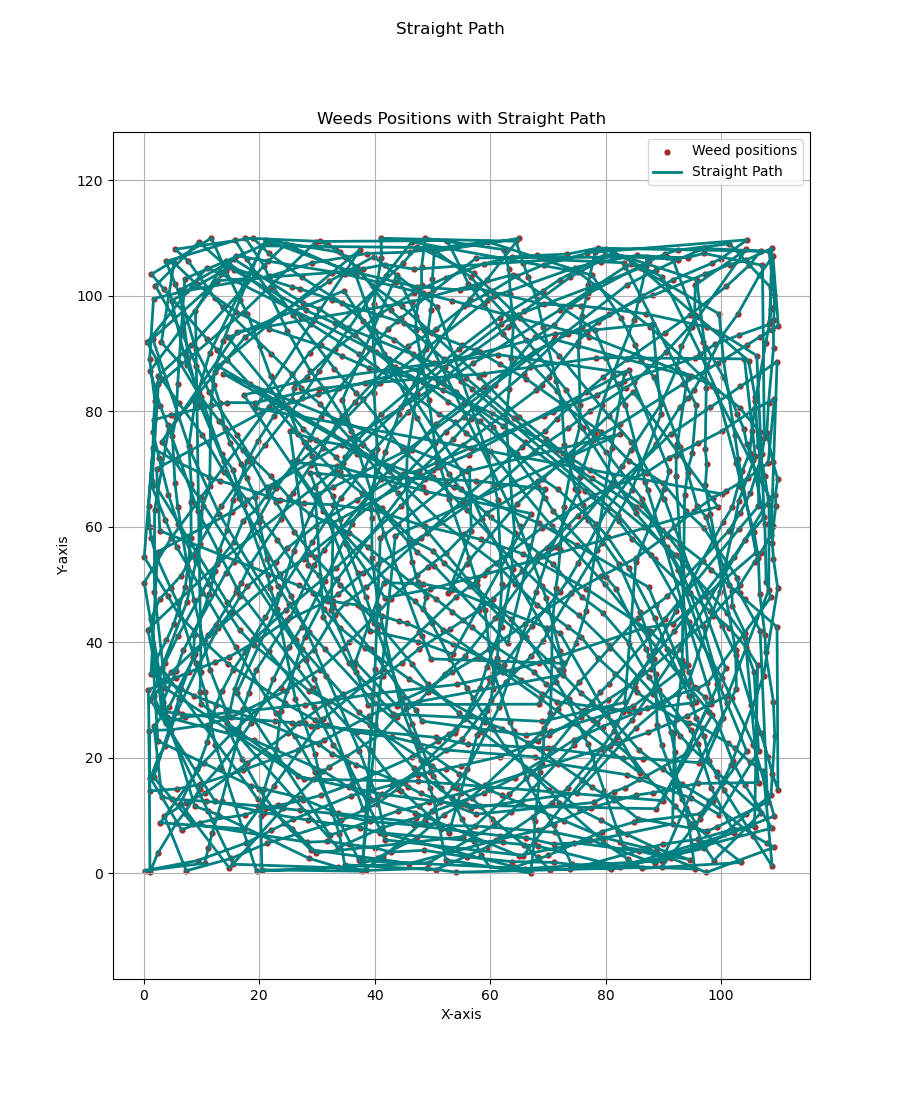
\includegraphics[height=36mm,width=0.24\textwidth]{Images/simulation_no_obs/straight_paths/21.png}
        & 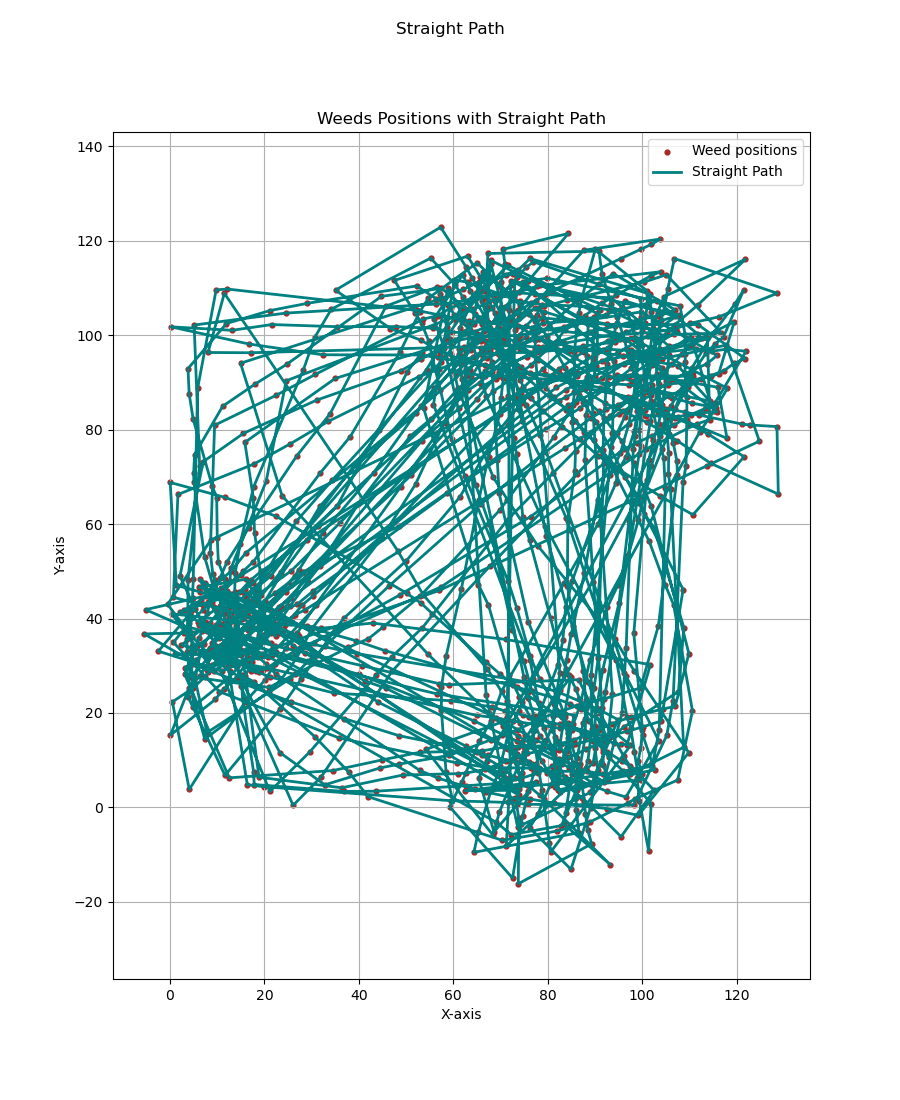
\includegraphics[height=36mm,width=0.24\textwidth]{Images/simulation_no_obs/straight_paths/22.png}
        & 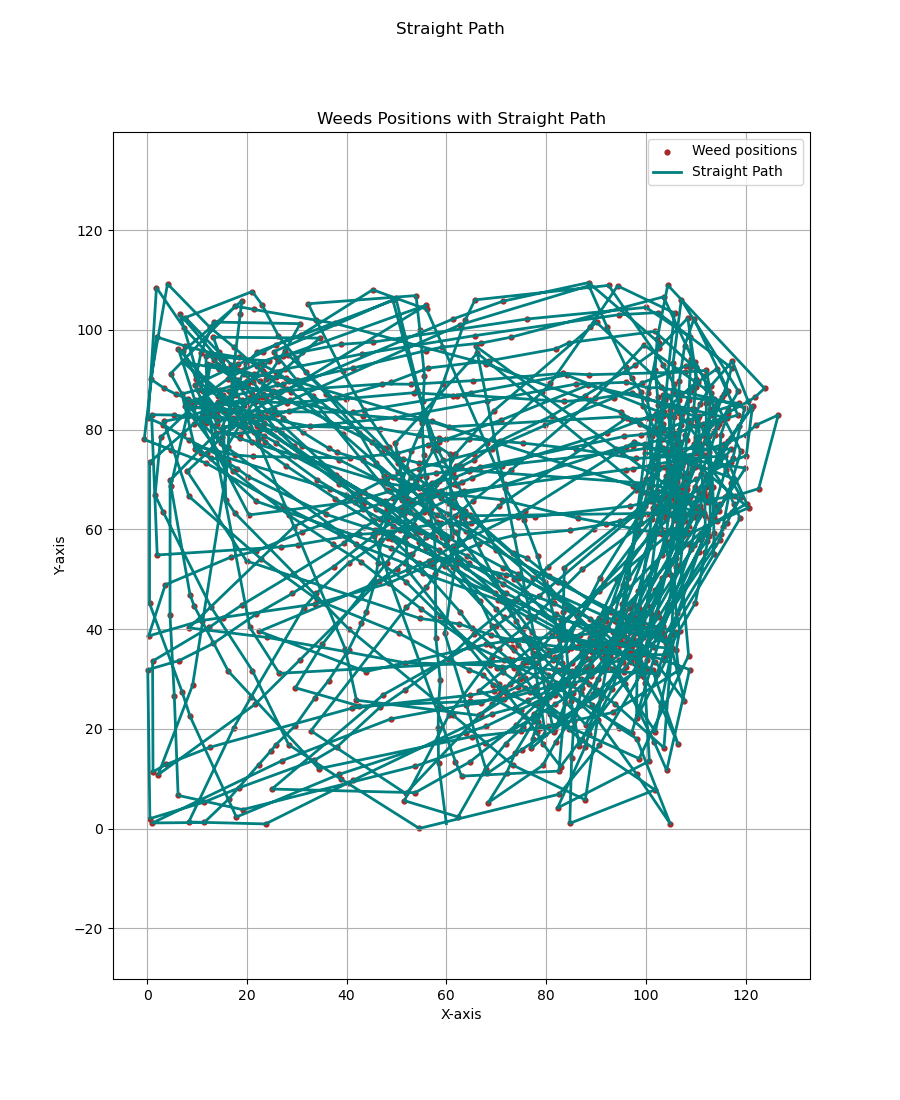
\includegraphics[height=36mm,width=0.24\textwidth]{Images/simulation_no_obs/straight_paths/23.png}
         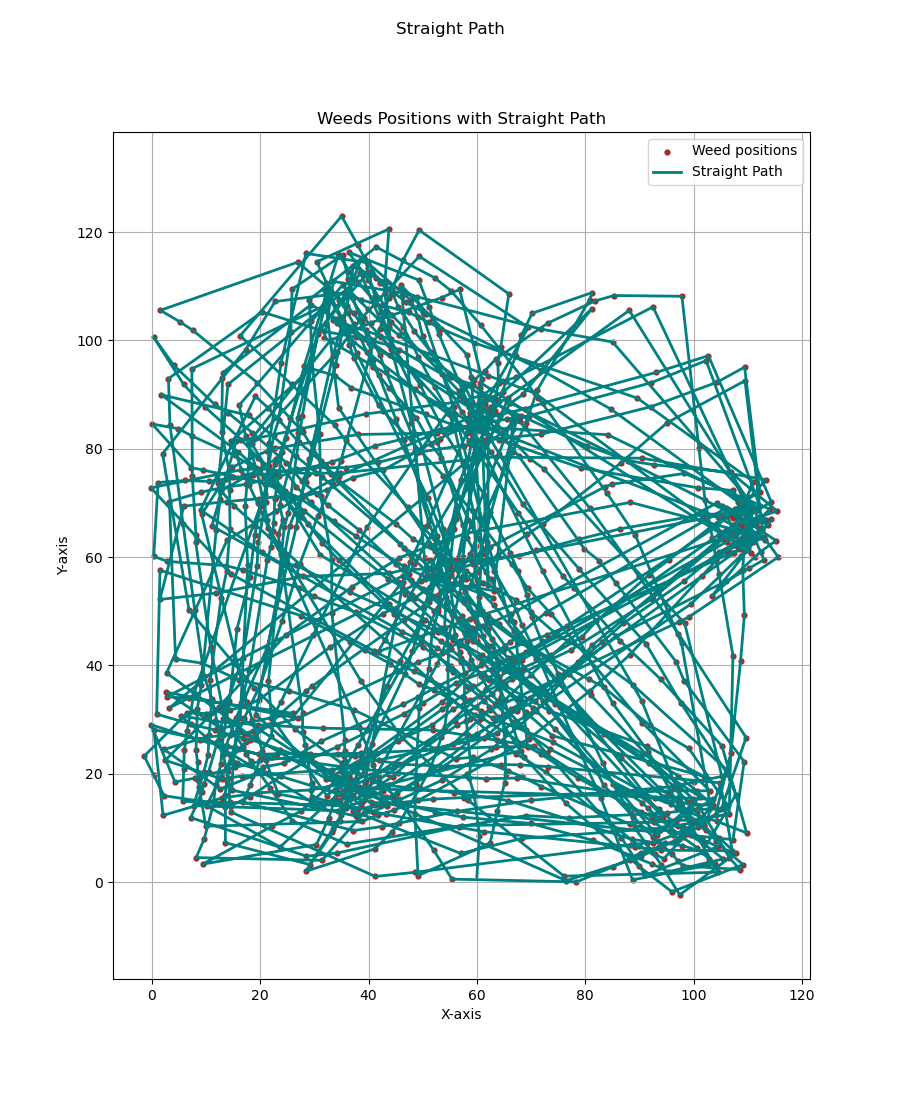
\includegraphics[height=36mm,width=0.24\textwidth]{Images/simulation_no_obs/straight_paths/24.png}\\[-4pt]

         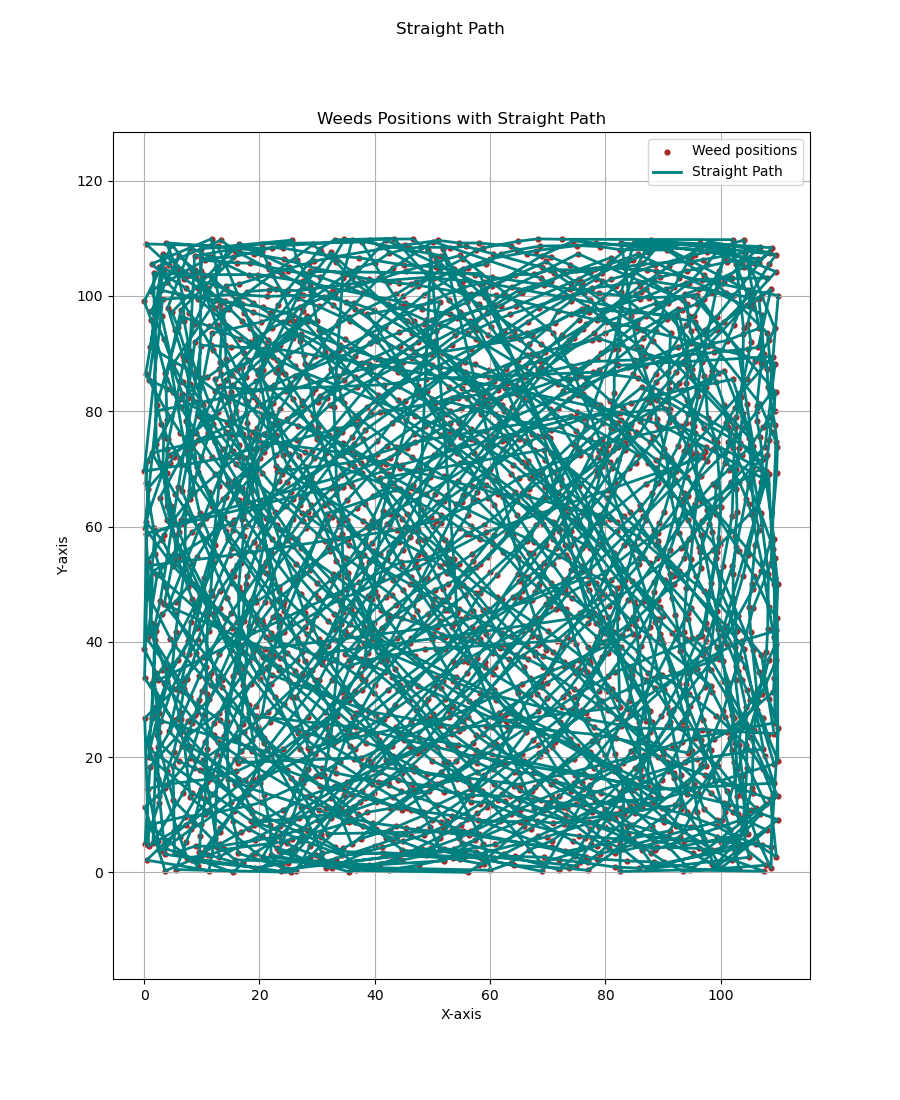
\includegraphics[height=36mm,width=0.24\textwidth]{Images/simulation_no_obs/straight_paths/31.png}
        & 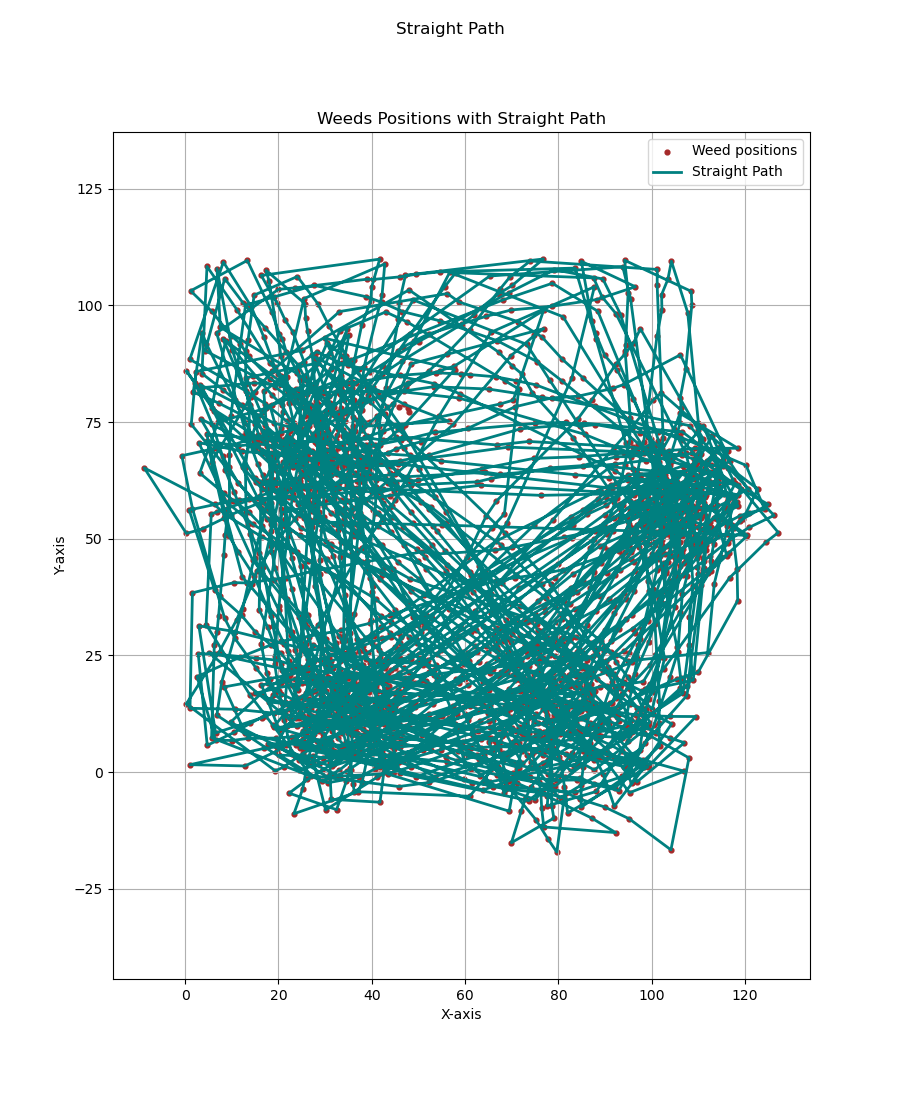
\includegraphics[height=36mm,width=0.24\textwidth]{Images/simulation_no_obs/straight_paths/32.png}
        & 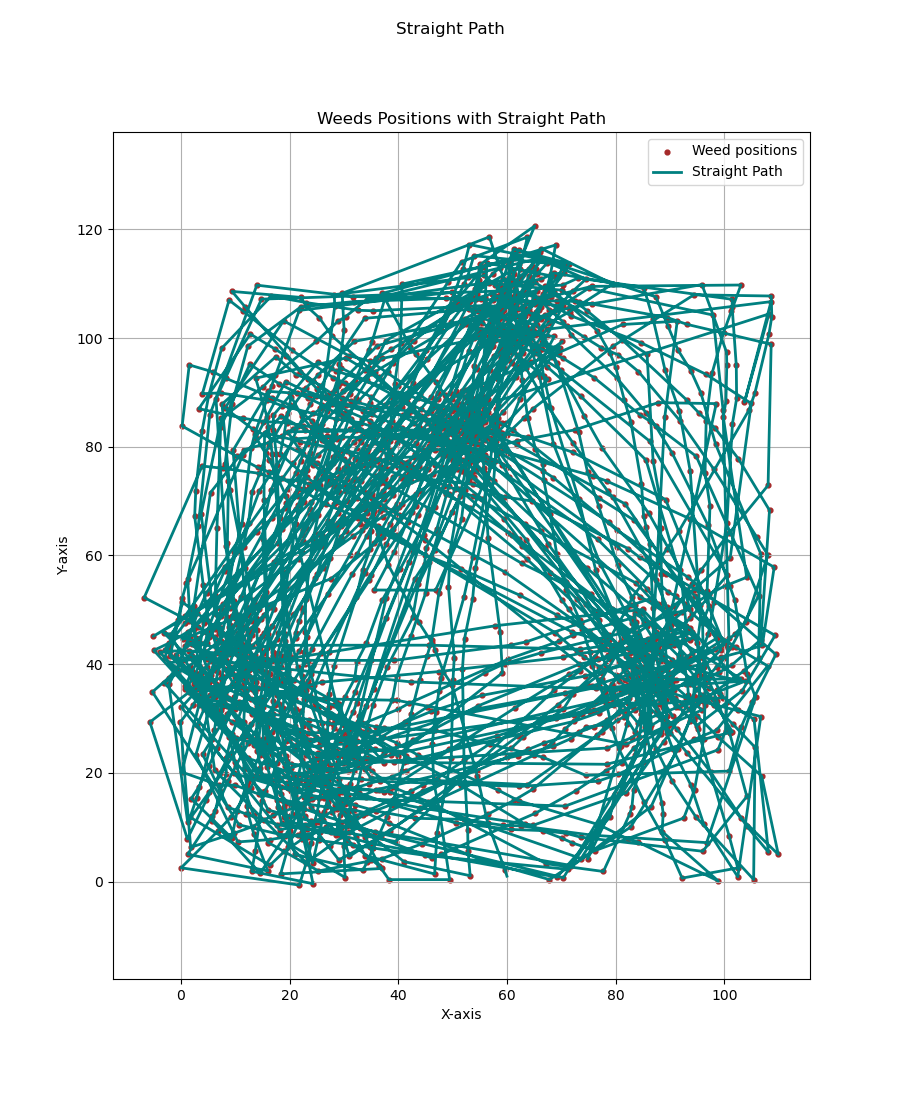
\includegraphics[height=36mm,width=0.24\textwidth]{Images/simulation_no_obs/straight_paths/33.png}
         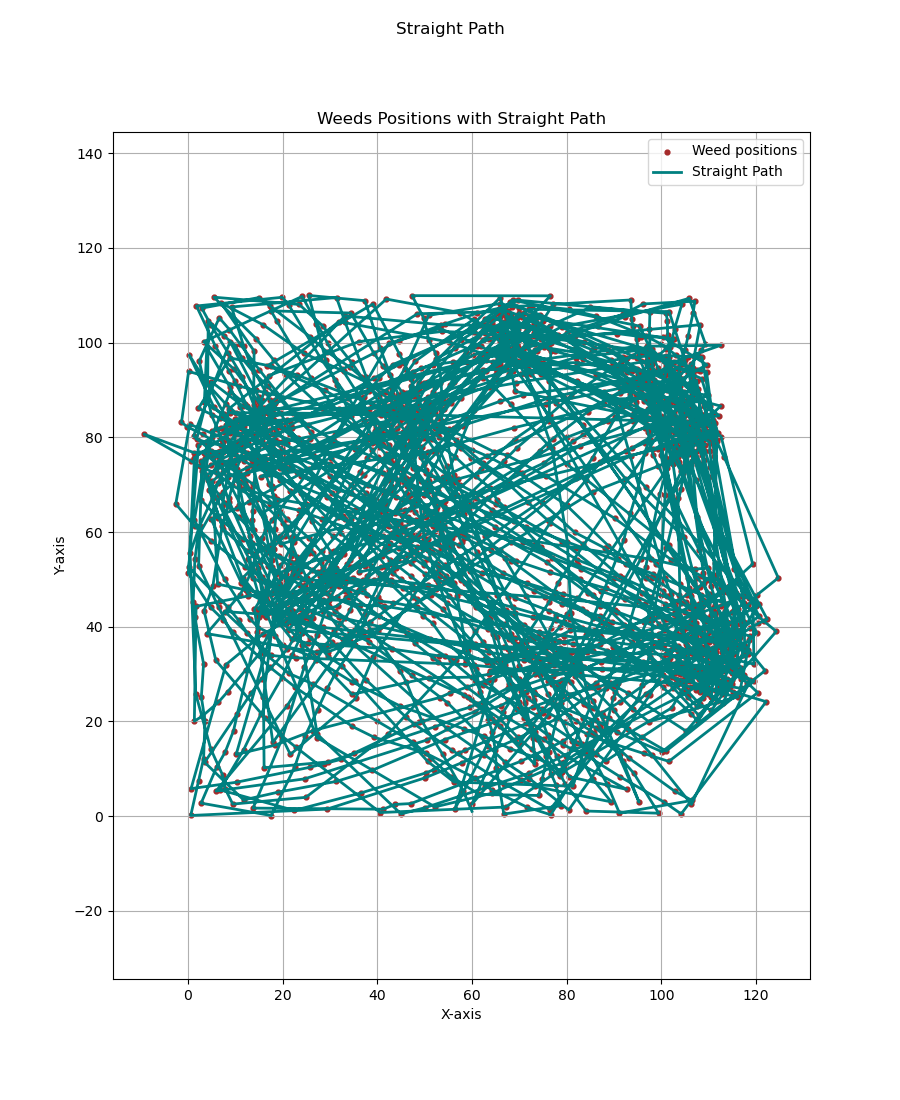
\includegraphics[height=36mm,width=0.24\textwidth]{Images/simulation_no_obs/straight_paths/34.png}\\[-4pt]


        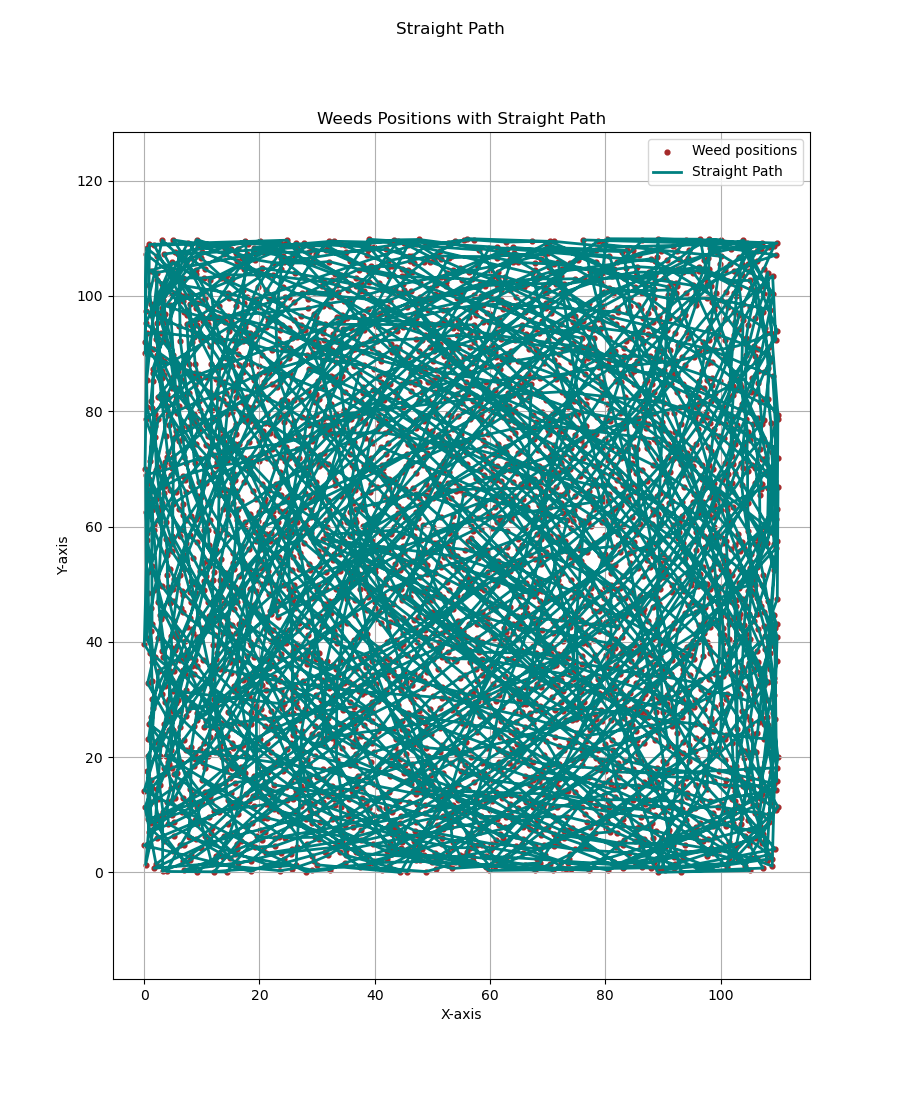
\includegraphics[height=36mm,width=0.24\textwidth]{Images/simulation_no_obs/straight_paths/41.png}
        & 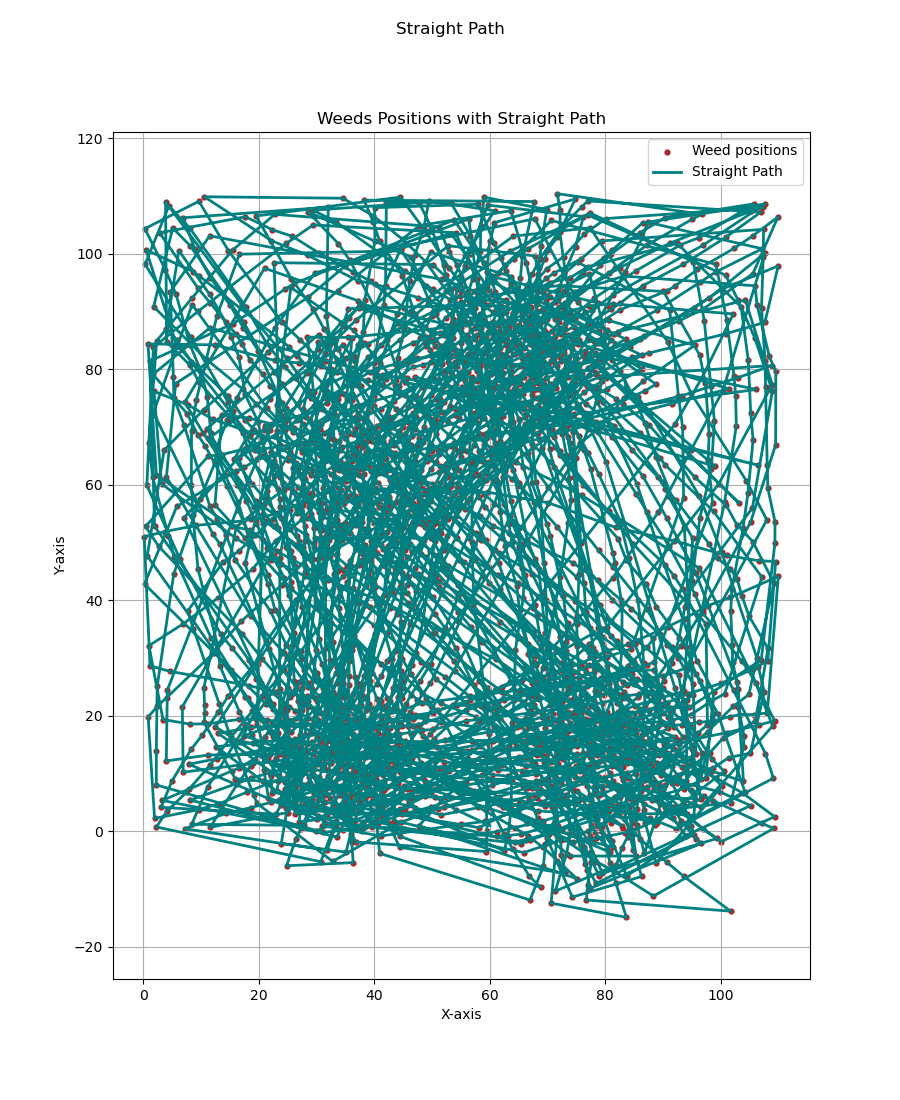
\includegraphics[height=36mm,width=0.24\textwidth]{Images/simulation_no_obs/straight_paths/42.png}
        & 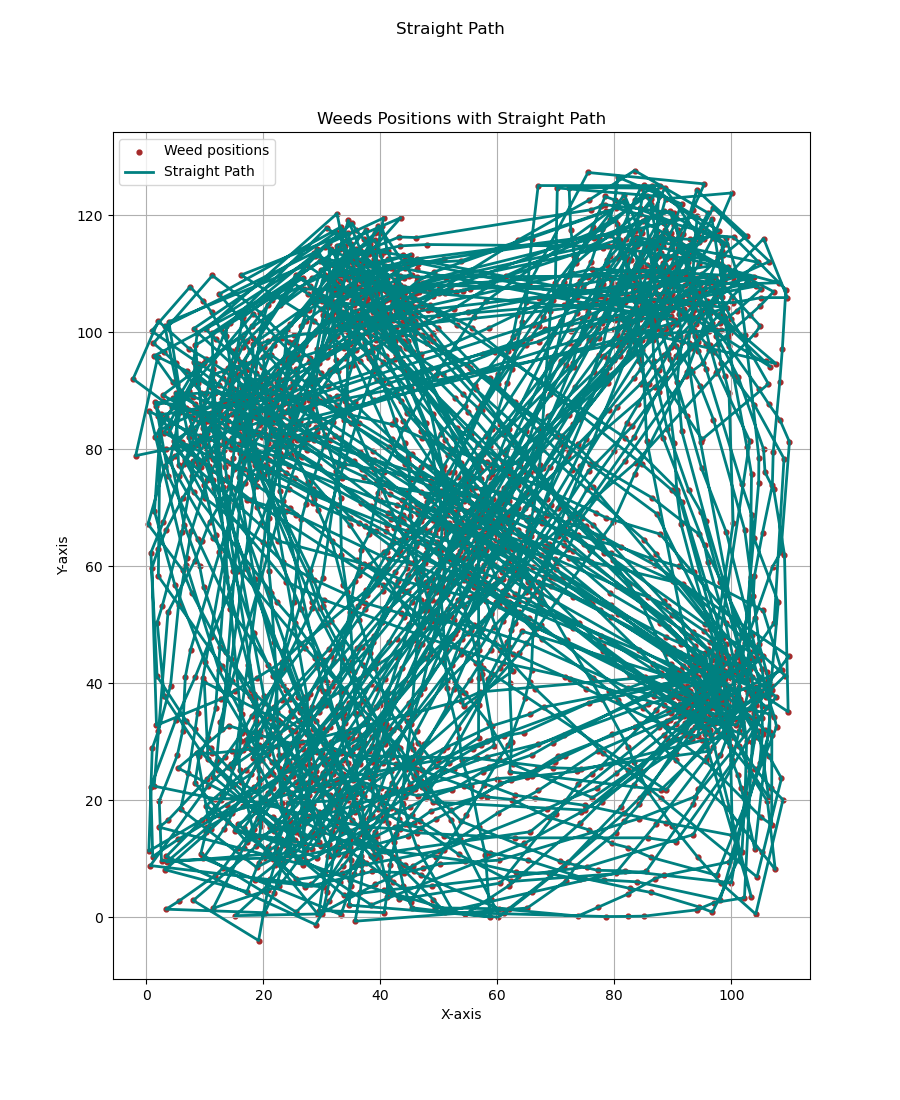
\includegraphics[height=36mm,width=0.24\textwidth]{Images/simulation_no_obs/straight_paths/43.png}
        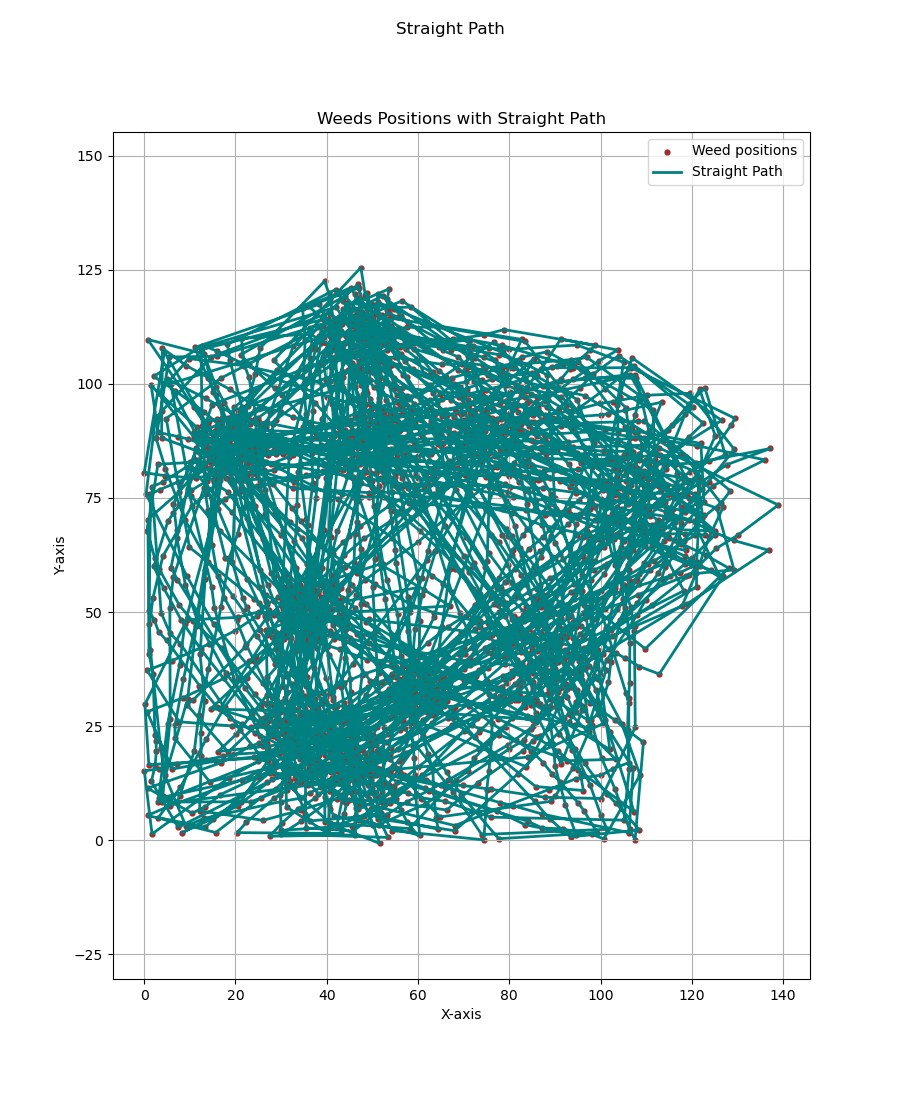
\includegraphics[height=36mm,width=0.24\textwidth]{Images/simulation_no_obs/straight_paths/44.png}\\[-4pt]

        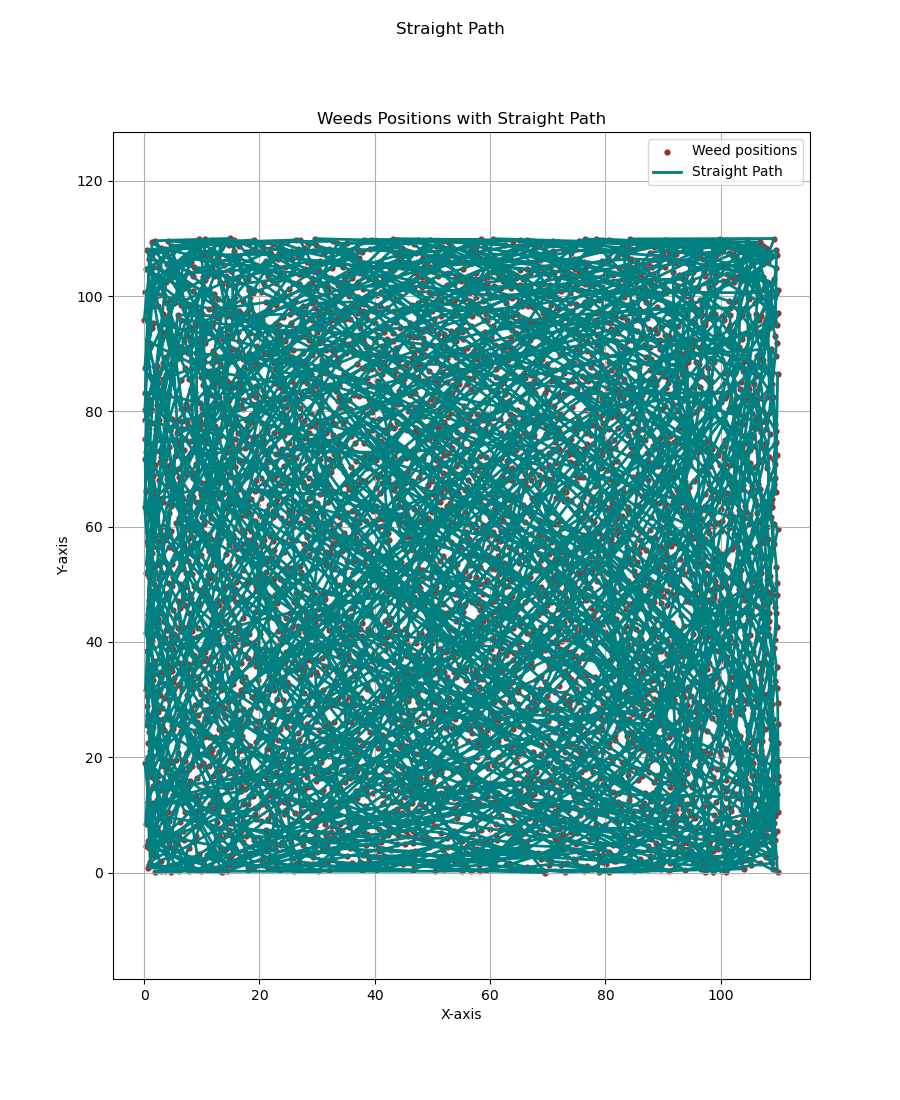
\includegraphics[height=36mm,width=0.24\textwidth]{Images/simulation_no_obs/straight_paths/51.png}
        & \includegraphics[height=36mm,width=0.24\textwidth]{Images/simulation_no_obs/straight_paths/52.png}
        & \includegraphics[height=36mm,width=0.24\textwidth]{Images/simulation_no_obs/straight_paths/53.png}
        \includegraphics[height=36mm,width=0.24\textwidth]{Images/simulation_no_obs/straight_paths/54.png}\\[-4pt]

    \end{tabular}
    \caption{Straight Path.\label{fig:straight_path}}
\end{figure}


\vspace{3mm}


Once the Dubins paths are generated from the straight paths, the resultant paths can be visualized in the (\autoref{fig:dubins_path}). These figures showcase the robot's traversal across different datasets, illustrating how the algorithm adapts to various point distributions.
% Dubin's path
\begin{figure}[p]
    \centering
    \begin{tabular}{ccc}
         \includegraphics[height=36mm,width=0.24\textwidth]{Images/simulation_no_obs/dubins_path/01.png}
        & \includegraphics[height=36mm,width=0.24\textwidth]{Images/simulation_no_obs/dubins_path/02.png}
        & \includegraphics[height=36mm,width=0.24\textwidth]{Images/simulation_no_obs/dubins_path/03.png}
         \includegraphics[height=36mm,width=0.24\textwidth]{Images/simulation_no_obs/dubins_path/04.png}\\[-4pt]

        \includegraphics[height=36mm,width=0.24\textwidth]{Images/simulation_no_obs/dubins_path/11.png}
        & \includegraphics[height=36mm,width=0.24\textwidth]{Images/simulation_no_obs/dubins_path/12.png}
        & \includegraphics[height=36mm,width=0.24\textwidth]{Images/simulation_no_obs/dubins_path/13.png}
        \includegraphics[height=36mm,width=0.24\textwidth]{Images/simulation_no_obs/dubins_path/14.png}\\[-4pt]

        \includegraphics[height=36mm,width=0.24\textwidth]{Images/simulation_no_obs/dubins_path/21.png}
        & \includegraphics[height=36mm,width=0.24\textwidth]{Images/simulation_no_obs/dubins_path/22.png}
        & \includegraphics[height=36mm,width=0.24\textwidth]{Images/simulation_no_obs/dubins_path/23.png}
         \includegraphics[height=36mm,width=0.24\textwidth]{Images/simulation_no_obs/dubins_path/24.png}\\[-4pt]

         \includegraphics[height=36mm,width=0.24\textwidth]{Images/simulation_no_obs/dubins_path/31.png}
        & \includegraphics[height=36mm,width=0.24\textwidth]{Images/simulation_no_obs/dubins_path/32.png}
        & \includegraphics[height=36mm,width=0.24\textwidth]{Images/simulation_no_obs/dubins_path/33.png}
         \includegraphics[height=36mm,width=0.24\textwidth]{Images/simulation_no_obs/dubins_path/34.png}\\[-4pt]


        \includegraphics[height=36mm,width=0.24\textwidth]{Images/simulation_no_obs/dubins_path/41.png}
        & \includegraphics[height=36mm,width=0.24\textwidth]{Images/simulation_no_obs/dubins_path/42.png}
        & \includegraphics[height=36mm,width=0.24\textwidth]{Images/simulation_no_obs/dubins_path/43.png}
        \includegraphics[height=36mm,width=0.24\textwidth]{Images/simulation_no_obs/dubins_path/44.png}\\[-4pt]

        \includegraphics[height=36mm,width=0.24\textwidth]{Images/simulation_no_obs/dubins_path/51.png}
        & \includegraphics[height=36mm,width=0.24\textwidth]{Images/simulation_no_obs/dubins_path/52.png}
        & \includegraphics[height=36mm,width=0.24\textwidth]{Images/simulation_no_obs/dubins_path/53.png}
        \includegraphics[height=36mm,width=0.24\textwidth]{Images/simulation_no_obs/dubins_path/54.png}\\[-4pt]

    \end{tabular}
    \caption{Dubin's Path.\label{fig:dubins_path}}
\end{figure}



\vspace{3mm}

The performance metrics for all datasets are summarized in the (\autoref{tab:performance_metrics}). These metrics provide insights into the algorithm's computational efficiency, operational effectiveness, and overall robustness.

% Metrics for CPP.
\begin{table}[]
    \centering
    \caption{Results for the performance metrics.}
    \label{tab:performance_metrics}
    \small
    \begin{tabular}{cllllll}
    \hline
    \rowcolor[HTML]{67D5DA} 
    \multicolumn{1}{l}{\cellcolor[HTML]{67D5DA}\textit{\textbf{\begin{tabular}[c]{@{}l@{}}No. of\\  points\end{tabular}}}} & \textit{\textbf{Cases}} & \textit{\textbf{\begin{tabular}[c]{@{}l@{}}Computation \\ Time in secs.\end{tabular}}} & \textit{\textbf{\begin{tabular}[c]{@{}l@{}}Field Operation\\  Time in sec.\end{tabular}}} & \textit{\textbf{\begin{tabular}[c]{@{}l@{}}Route length\\  in meters\end{tabular}}} & \textit{\textbf{\begin{tabular}[c]{@{}l@{}}No. of \\ Turns.\end{tabular}}} & \textit{\textbf{\begin{tabular}[c]{@{}l@{}}Energy \\ Consumption \\ in KWh.\end{tabular}}} \\ \hline
    \rowcolor[HTML]{FFFFC7} 
    \cellcolor[HTML]{FFFFC7}                                                                                               & case 1                  & 0.858553886                                                                            & 6282.400938                                                                               & 4652.945                                                                            & 48                                                                         & 5783.34459                                                                                 \\ \cline{2-7} 
    \rowcolor[HTML]{FFFFC7} 
    \cellcolor[HTML]{FFFFC7}                                                                                               & case 2                  & 0.775789261                                                                            & 5125.168209                                                                               & 3769.005                                                                            & 41                                                                         & 4734.555207                                                                                \\ \cline{2-7} 
    \rowcolor[HTML]{FFFFC7} 
    \cellcolor[HTML]{FFFFC7}                                                                                               & case 3                  & 0.788151503                                                                            & 5413.822753                                                                               & 3985.978                                                                            & 44                                                                         & 5022.177564                                                                                \\ \cline{2-7} 
    \rowcolor[HTML]{FFFFC7} 
    \multirow{-4}{*}{\cellcolor[HTML]{FFFFC7}250}                                                                          & case 4                  & 0.825942278                                                                            & 6216.01818                                                                                & 4620.695                                                                            & 44                                                                         & 5656.894864                                                                                \\ \hline
    \rowcolor[HTML]{FFFFC7} 
    \cellcolor[HTML]{FFFFC7}                                                                                               & case 1                  & 1.842700005                                                                            & 9520.140257                                                                               & 7027.363                                                                            & 75                                                                         & 8793.612844                                                                                \\ \cline{2-7} 
    \rowcolor[HTML]{FFFFC7} 
    \cellcolor[HTML]{FFFFC7}                                                                                               & case 2                  & 1.696401358                                                                            & 9151.211911                                                                               & 6788.619                                                                            & 67                                                                         & 8366.468569                                                                                \\ \cline{2-7} 
    \rowcolor[HTML]{FFFFC7} 
    \cellcolor[HTML]{FFFFC7}                                                                                               & case 3                  & 1.940592766                                                                            & 8589.717644                                                                               & 6336.544                                                                            & 67                                                                         & 7914.394434                                                                                \\ \cline{2-7} 
    \rowcolor[HTML]{FFFFC7} 
    \multirow{-4}{*}{\cellcolor[HTML]{FFFFC7}500}                                                                          & case 4                  & 1.609200478                                                                            & 9761.624722                                                                               & 7250.2                                                                              & 70                                                                         & 8898.700417                                                                                \\ \hline
    \rowcolor[HTML]{FFFFC7} 
    \cellcolor[HTML]{FFFFC7}                                                                                               & case 1                  & 9.04812026                                                                             & 21751.64778                                                                               & 16189.858                                                                           & 154                                                                        & 19816.55759                                                                                \\ \cline{2-7} 
    \rowcolor[HTML]{FFFFC7} 
    \cellcolor[HTML]{FFFFC7}                                                                                               & case 2                  & 8.591621161                                                                            & 22226.37676                                                                               & 16650.701                                                                           & 144                                                                        & 20041.90077                                                                                \\ \cline{2-7} 
    \rowcolor[HTML]{FFFFC7} 
    \cellcolor[HTML]{FFFFC7}                                                                                               & case 3                  & 7.65038085                                                                             & 18446.73883                                                                               & 13728.721                                                                           & 131                                                                        & 16813.77138                                                                                \\ \cline{2-7} 
    \rowcolor[HTML]{FFFFC7} 
    \multirow{-4}{*}{\cellcolor[HTML]{FFFFC7}2000}                                                                         & case 4                  & 8.155776024                                                                            & 20839.67217                                                                               & 15547.469                                                                           & 139                                                                        & 18820.91894                                                                                \\ \hline
    \rowcolor[HTML]{FFFFC7} 
    \cellcolor[HTML]{FFFFC7}                                                                                               & case 1                  & 24.18394971                                                                            & 32301.69933                                                                               & 24191.259                                                                           & 210                                                                        & 29136.75914                                                                                \\ \cline{2-7} 
    \rowcolor[HTML]{FFFFC7} 
    \cellcolor[HTML]{FFFFC7}                                                                                               & case 2                  & 20.85941482                                                                            & 29871.08874                                                                               & 22356.011                                                                           & 198                                                                        & 27018.91147                                                                                \\ \cline{2-7} 
    \rowcolor[HTML]{FFFFC7} 
    \cellcolor[HTML]{FFFFC7}                                                                                               & case 3                  & 18.23963118                                                                            & 27659.4681                                                                                & 20620.054                                                                           & 192                                                                        & 25141.65448                                                                                \\ \cline{2-7} 
    \rowcolor[HTML]{FFFFC7} 
    \multirow{-4}{*}{\cellcolor[HTML]{FFFFC7}4000}                                                                         & case 4                  & 19.22349644                                                                            & 29701.58872                                                                               & 22222.31                                                                            & 200                                                                        & 26932.31049                                                                                \\ \hline
    \rowcolor[HTML]{FFFFC7} 
    \cellcolor[HTML]{FFFFC7}                                                                                               & case 1                  & 45.23673987                                                                            & 39851.80224                                                                               & 29777.382                                                                           & 262                                                                        & 35947.48179                                                                                \\ \cline{2-7} 
    \rowcolor[HTML]{FFFFC7} 
    \cellcolor[HTML]{FFFFC7}                                                                                               & case 2                  & 33.23154497                                                                            & 34821.16749                                                                               & 26039.854                                                                           & 236                                                                        & 31597.65399                                                                                \\ \cline{2-7} 
    \rowcolor[HTML]{FFFFC7} 
    \cellcolor[HTML]{FFFFC7}                                                                                               & case 3                  & 30.80121374                                                                            & 35035.83592                                                                               & 26223.169                                                                           & 230                                                                        & 31639.66906                                                                                \\ \cline{2-7} 
    \rowcolor[HTML]{FFFFC7} 
    \multirow{-4}{*}{\cellcolor[HTML]{FFFFC7}6000}                                                                         & case 4                  & 32.34737062                                                                            & 35496.36509                                                                               & 26570.832                                                                           & 226                                                                        & 31893.13207                                                                                \\ \hline
    \rowcolor[HTML]{FFFFC7} 
    \cellcolor[HTML]{FFFFC7}                                                                                               & case 1                  & 122.6808474                                                                            & 50681.89334                                                                               & 38128.675                                                                           & 308                                                                        & 45382.07468                                                                                \\ \cline{2-7} 
    \rowcolor[HTML]{FFFFC7} 
    \cellcolor[HTML]{FFFFC7}                                                                                               & case 2                  & 74.37674475                                                                            & 45367.87779                                                                               & 34118.252                                                                           & 277                                                                        & 40641.60223                                                                                \\ \cline{2-7} 
    \rowcolor[HTML]{FFFFC7} 
    \cellcolor[HTML]{FFFFC7}                                                                                               & case 3                  & 65.54510021                                                                            & 42291.24514                                                                               & 31650.696                                                                           & 278                                                                        & 38197.59611                                                                                \\ \cline{2-7} 
    \rowcolor[HTML]{FFFFC7} 
    \multirow{-4}{*}{\cellcolor[HTML]{FFFFC7}10000}                                                                        & case 4                  & 62.76576424                                                                            & 42801.16425                                                                               & 32154.031                                                                           & 274                                                                        & 38606.73138                                                                                \\ \hline
    \end{tabular}
    \end{table}



\vspace{3mm} 


The coverage rate plot over the field time offers a visual representation of the algorithm's performance across the whole datasets. This plot demonstrates how effectively the algorithm achieves coverage over time, allowing for a comparative analysis of its efficiency under varying point distributions and densities. This plot can be visualized in (\autoref{fig:coverage_plots}).   

% Coverage rate plot
\begin{figure}[p]
    \centering
    \begin{tabular}{ccc}
         \includegraphics[height=36mm,width=0.24\textwidth]{Images/simulation_no_obs/coverage_plots/01.png}
        & \includegraphics[height=36mm,width=0.24\textwidth]{Images/simulation_no_obs/coverage_plots/02.png}
        & \includegraphics[height=36mm,width=0.24\textwidth]{Images/simulation_no_obs/coverage_plots/03.png}
         \includegraphics[height=36mm,width=0.24\textwidth]{Images/simulation_no_obs/coverage_plots/04.png}\\[-4pt]

        \includegraphics[height=36mm,width=0.24\textwidth]{Images/simulation_no_obs/coverage_plots/11.png}
        & \includegraphics[height=36mm,width=0.24\textwidth]{Images/simulation_no_obs/coverage_plots/12.png}
        & \includegraphics[height=36mm,width=0.24\textwidth]{Images/simulation_no_obs/coverage_plots/13.png}
        \includegraphics[height=36mm,width=0.24\textwidth]{Images/simulation_no_obs/coverage_plots/14.png}\\[-4pt]

        \includegraphics[height=36mm,width=0.24\textwidth]{Images/simulation_no_obs/coverage_plots/21.png}
        & \includegraphics[height=36mm,width=0.24\textwidth]{Images/simulation_no_obs/coverage_plots/22.png}
        & \includegraphics[height=36mm,width=0.24\textwidth]{Images/simulation_no_obs/coverage_plots/23.png}
         \includegraphics[height=36mm,width=0.24\textwidth]{Images/simulation_no_obs/coverage_plots/24.png}\\[-4pt]

         \includegraphics[height=36mm,width=0.24\textwidth]{Images/simulation_no_obs/coverage_plots/31.png}
        & \includegraphics[height=36mm,width=0.24\textwidth]{Images/simulation_no_obs/coverage_plots/32.png}
        & \includegraphics[height=36mm,width=0.24\textwidth]{Images/simulation_no_obs/coverage_plots/33.png}
         \includegraphics[height=36mm,width=0.24\textwidth]{Images/simulation_no_obs/coverage_plots/34.png}\\[-4pt]


        \includegraphics[height=36mm,width=0.24\textwidth]{Images/simulation_no_obs/coverage_plots/41.png}
        & \includegraphics[height=36mm,width=0.24\textwidth]{Images/simulation_no_obs/coverage_plots/42.png}
        & \includegraphics[height=36mm,width=0.24\textwidth]{Images/simulation_no_obs/coverage_plots/43.png}
        \includegraphics[height=36mm,width=0.24\textwidth]{Images/simulation_no_obs/coverage_plots/44.png}\\[-4pt]

        \includegraphics[height=36mm,width=0.24\textwidth]{Images/simulation_no_obs/coverage_plots/51.png}
        & \includegraphics[height=36mm,width=0.24\textwidth]{Images/simulation_no_obs/coverage_plots/52.png}
        & \includegraphics[height=36mm,width=0.24\textwidth]{Images/simulation_no_obs/coverage_plots/53.png}
        \includegraphics[height=36mm,width=0.24\textwidth]{Images/simulation_no_obs/coverage_plots/54.png}\\[-4pt]

    \end{tabular}
    \caption{Coverage plots.\label{fig:coverage_plots}}
    \end{figure}


The performance metrics plots provide a visual representation for better understanding of the algorithm's performance across different datasets. Therefore, separate plots for each performance metric are generated to analyze the algorithm's performance under varying scenarios. These plots can be visualized in the (\autoref{fig:Computation_time}), (\autoref{fig:Energy_expenditure}), (\autoref{fig:Route_length}), and (\autoref{fig:Field_operation_time}).


\begin{figure}[H]
    \centering
    \includegraphics[width=\textwidth]{Images/plots/no_obs/Computation_time.png}
    \caption{Computation Time.}
    \label{fig:Computation_time}
\end{figure}

\begin{figure}[H]
    \centering
    \includegraphics[width=\textwidth]{Images/plots/no_obs/Energy.png}
    \caption{Energy Expenditure.}
    \label{fig:Energy_expenditure}
\end{figure}

\begin{figure}[H]
    \centering
    \includegraphics[width=\textwidth]{Images/plots/no_obs/Route_length.png}
    \caption{Route Length.}
    \label{fig:Route_length}
\end{figure}

\begin{figure}[H]
    \centering
    \includegraphics[width=\textwidth]{Images/plots/no_obs/Field_time.png}
    \caption{Field Operation Time.}
    \label{fig:Field_operation_time}
\end{figure}


The proposed algorithm operates by initially generating straight paths and subsequently applying Dubins paths to ensure feasibility given the robot's constraints. The straight paths, as visualized in the initial results, are approximately linear, aiming to cover the maximum number of points while maintaining minimal path length. This demonstrates the algorithm's ability to generate efficient coverage paths.

\vspace{3mm} 

The Dubins path results further validate the algorithm's capability to model the robot's constraints effectively. An inability to model these constraints accurately would result in numerous infeasible circular paths. The primary objective of employing this behavioral approach is to sustain a high coverage rate from start to finish across various data distributions. The results indicate that the algorithm successfully maintains a high coverage rate irrespective of the distribution type. It is noteworthy that the coverage rate is initially very high and gradually decreases, attributed to the diminishing number of points left to cover after a significant percentage of coverage. Nonetheless, the coverage rate remains high, indicating efficient coverage by the algorithm. The percentage coverage also suggests that the point at which the algorithm changes behavior is near-optimal; otherwise, a gradual increase in coverage rate would be observed if the change occurred at a different percentage.

\vspace{3mm} 

The computation time plot across all datasets indicates an expected increase in computation time with the number of points. However, the rise in computation time is notable. For instance, even in the largest case of 10,000 points with random distribution, the computation time is 122.68 seconds, which is remarkably low as compared to current state-of-the-art approaches following the non-holonoomic constraints. This efficiency is further highlighted by the average computation time of 60 seconds for other scenarios, demonstrating the algorithm's computational efficiency. This is particularly significant as no real agricultural field would have a purely random distribution, making the algorithm's performance even more impressive in practical scenarios.

\vspace{3mm} 

Similarly, the route length increases with the number of points as the robot needs to traverse more straight lines to cover all points. It is noteworthy that the maximum route length for each dataset occurs with random distribution and decreases significantly with fewer clusters, increasing again as the number of clusters rises.

\vspace{3mm} 

Field operation time and energy consumption are derived from the route length, factoring in the robot's maximum allowable velocity on straight and curved paths. The robot can move at twice the speed on straight paths compared to curved paths without damaging crops. The parameters used for the current robot, as outlined in the table, provide a close approximation of real values, although the exact curved distance is challenging to estimate with this pipeline. Energy consumption is approximated to be four times higher on curved paths than on straight paths. The plots above reflect these estimations. 


 
% \newpage 

% 
\chapter{Simulation Test and Analysis with obstacles} 


This section presents a comprehensive examination of the proposed complete coverage path planning algorithm, tailored to handle static polygonal obstacles in agricultural field applications. The section is divided into two key parts: Simulation Setup and Results \& Analysis.

\section{Simulation Setup}

This subsection provides a detailed description of the simulation setup, focusing on the experimental framework within which the tests are conducted.

\vspace{3mm}  


The simulation environment is meticulously crafted to replicate real-world agricultural fields, incorporating static polygonal obstacles to simulate common structures such as trees, rocks, or buildings that serve as keep-out zones. This realistic setup ensures that the algorithm's performance is rigorously evaluated under practical conditions.

\vspace{3mm}  

This simulation environment is setup utilizing a realistic field data obtained from the field manually and inclusion of the obstacles within the field. While the point distribution remains unchanged, the obstacles' shapes, sizes, and numbers vary across different scenarios. Strategic placement of obstacles tests the algorithm's adaptability and robustness. Five distinct datasets are used to assess the algorithm's performance under varying obstacle configurations, increasing in complexity with each set.



\vspace{3mm}  

Dataset Description

To thoroughly evaluate the algorithm, five distinct datasets are employed within a flat 120m x 120m field, each containing different numbers and configurations of obstacles:

\begin{itemize}
    \item Set1: Contains one rectangular obstacle of size 10m x 10m.
    \item Set2: Contains two rectangular obstacles of sizes 10m x 10m and 4m x 4m.
    \item Set3: Contains three convex polygonal obstacles of distinct sizes and shapes.
    \item Set4: Contains six convex polygonal obstacles of different sizes and shapes.
    \item Set5: Contains six polygonal obstacles of varying sizes and shapes, including concave and extremely long obstacles.
\end{itemize}
This hierarchical arrangement of datasets, with increasing complexity, ensures comprehensive testing of the algorithm's robustness and adaptability to real-world agricultural environments, where obstacles can vary significantly.

\vspace{3mm}  

Performance Metrics
The algorithm's performance is evaluated using several critical metrics across all datasets:

\begin{itemize}
    \item Computational Time: The time required for the algorithm to compute the coverage path.
    \item Field Operation Time: The actual time taken for the robot to complete the coverage task.
    \item Total Path Length: The total distance traveled by the robot.
    \item Number of Turns: The total number of turns the robot makes during its operation.
    \item Energy Consumption: The energy used by the robot to complete the coverage task.
    \item Coverage Efficiency: The percentage of points covered by the robot within the operational time.
\end{itemize}
These metrics provide a comprehensive assessment of the algorithm's efficiency, effectiveness, and overall performance under different test scenarios.


\vspace{3mm}  

\textbf{Visual Representation of the Dataset}

The (\autoref{fig:obstacles_dataset}) illustrates the five different datasets used in the simulation experiments, showcasing the shapes, sizes, numbers, and locations of obstacles within the field. This visual representation aids in understanding the varying complexities introduced by the obstacles.


% % % % Dataset image
\begin{figure}[htbp]
    \centering
    \begin{tabular}{ccc}
         \includegraphics[height=36mm,width=0.24\textwidth]{Images/simulation_obs/Data/1.png}
        & \includegraphics[height=36mm,width=0.24\textwidth]{Images/simulation_obs/Data/2.png}
         \includegraphics[height=36mm,width=0.24\textwidth]{Images/simulation_obs/Data/3.png}\\[-4pt]

        \includegraphics[height=36mm,width=0.24\textwidth]{Images/simulation_obs/Data/4.png}
        & \includegraphics[height=36mm,width=0.24\textwidth]{Images/simulation_obs/Data/5.png}

    \end{tabular}
    \caption{Obstacles Dataset.\label{fig:obstacles_dataset}}
\end{figure}



\section{Simulation Results and Analysis}

This section details the results and analysis of simulation experiments designed to evaluate the robustness of the proposed complete coverage path planning algorithm in the presence of static polygonal obstacles. The empirical findings are meticulously analyzed to provide insights into the algorithm's performance across diverse scenarios, offering a comprehensive assessment of its efficiency and effectiveness.

\vspace{3mm}  

\textbf{Experimental Consistency}
To ensure the validity of comparisons and isolate the effects of different datasets on the algorithm's performance, the initial position and orientation of the robot were kept constant throughout all experiments. Additionally, the parameters for both the robot and the algorithm were consistently maintained across all trials.

\vspace{3mm}  

\textbf{Robot Constraints and Algorithm Parameters: } 


The robot's constraints and operational parameters are set to realistic values to ensure the validity of the simulation results. These data can be visualized in (\autoref{tab:constraints_and_parameters_obs}).

% % % % Table robot parameters 1
\begin{table}[]
    \centering
    \caption{Constraints and Parameters in presence of obstacles.}
    \label{tab:constraints_and_parameters_obs}
    \begin{tabular}{|c|c|}
    \hline
    \rowcolor[HTML]{FFCC67} 
    \textit{\textbf{Constraints and Parameters}}                                    & \textit{\textbf{Values}}       \\ \hline
    \rowcolor[HTML]{CBF9FC} 
    \textit{Robot initial position}                                                 & {[}60.0, 1.0{]}                \\ \hline
    \rowcolor[HTML]{CBF9FC} 
    \textit{Robot initial orientation}                                              & 45                             \\ \hline
    \rowcolor[HTML]{CBF9FC} 
    \textit{Search angle of the vision cone}                                        & ±11                            \\ \hline
    \rowcolor[HTML]{CBF9FC} 
    \textit{Minimum search radius of the vision cone.}                              & 1.25                           \\ \hline
    \rowcolor[HTML]{CBF9FC} 
    \textit{Maximum search radius of the vision cone.}                              & 100                            \\ \hline
    \rowcolor[HTML]{CBF9FC} 
    \textit{Minimum turning radius allowed for the robot.}                          & 2.0                            \\ \hline
    \rowcolor[HTML]{CBF9FC} 
    \textit{robot velocity on curved paths.}                                        & 0.4                            \\ \hline
    \rowcolor[HTML]{CBF9FC} 
    \textit{robot velocity on straight paths.}                                      & 0.8                            \\ \hline
    \rowcolor[HTML]{CBF9FC} 
    \textit{Distance used to compute field time taken on curved paths.}             & 7.85                           \\ \hline
    \rowcolor[HTML]{CBF9FC} 
    \textit{Number of points to consider in the vision cone.}                       & 5                              \\ \hline
    \rowcolor[HTML]{CBF9FC} 
    \textit{Minimum distance between intermediate points, and start and end point.} & 2.7                            \\ \hline
    \rowcolor[HTML]{CBF9FC} 
    \textit{Minimum distance between intermediate points.}                          & 2                              \\ \hline
    \rowcolor[HTML]{CBF9FC} 
    \textit{Maximum distance of the intermediate point form the path.}              & 0.6                            \\ \hline
    \rowcolor[HTML]{CBF9FC} 
    \textit{Graph search extreme angles}                                            & ±11                            \\ \hline
    \rowcolor[HTML]{CBF9FC} 
    \textit{buffer distance around obstacles.}                                      & 1                              \\ \hline
    \rowcolor[HTML]{CBF9FC} 
    \textit{Extend polygon distance for safe region.}                               & 1.4                            \\ \hline
    \rowcolor[HTML]{CBF9FC} 
    \textit{Graph generation step reduction iteration.}                             & 3                              \\ \hline
    \rowcolor[HTML]{CBF9FC} 
    \textit{Grid diameter.}                                                         & 0.4                            \\ \hline
    \rowcolor[HTML]{CBF9FC} 
    \textit{Max generation for graph generation.}                                   & 18                             \\ \hline
    \rowcolor[HTML]{CBF9FC} 
    \textit{Minimum step length for graph generation.}                              & 1.2                            \\ \hline
    \rowcolor[HTML]{CBF9FC} 
    \textit{Total operational area.}                                                & {[}{[}-2,0{]}, {[}90,120{]}{]} \\ \hline
    \rowcolor[HTML]{CBF9FC} 
    \textit{Distance between waypoints.}                                            & 10                             \\ \hline
    \end{tabular}
    \end{table}


The algorithm parameters are also meticulously defined to ensure consistent performance across all experiments. These parameters are set based on the robot's physical constraints and operational requirements, ensuring that the algorithm operates within realistic boundaries.

\vspace{3mm} 

The algorithm was designed to initially compute the global coverage path using straight lines. Subsequently, Dubins paths are generated for each line segment to ensure the shortest feasible path between each pair of points, optimizing the overall path length. The (\autoref{fig:straight_path_obs}) illustrate the straight obstacle free paths generated by the algorithm for all the datasets.

% % % % Straight_path with obstacles   
\begin{figure}[]
    \centering
    \begin{tabular}{ccc} 
         \includegraphics[height=36mm,width=0.24\textwidth]{Images/simulation_obs/obs_straight/1.png}
        & \includegraphics[height=36mm,width=0.24\textwidth]{Images/simulation_obs/obs_straight/2.png}
         \includegraphics[height=36mm,width=0.24\textwidth]{Images/simulation_obs/obs_straight/3.png}\\[-4pt]

        \includegraphics[height=36mm,width=0.24\textwidth]{Images/simulation_obs/obs_straight/4.png}
        & \includegraphics[height=36mm,width=0.24\textwidth]{Images/simulation_obs/obs_straight/5.png} 

    \end{tabular}
    \caption{Straight Path.\label{fig:straight_path_obs}}
\end{figure}


\vspace{3mm}

The resulting path after applying dubins constraints are depicted in the (\autoref{fig:dubins_path_obs}). These visual representations portray the robot's movement across diverse datasets, providing insight into the algorithm's adaptability amidst varying obstacles. 



% % % % Dubins_path with obstacles   
\begin{figure}[htbp]
    \centering
    \begin{tabular}{ccc} 
         \includegraphics[height=36mm,width=0.24\textwidth]{Images/simulation_obs/obs_dubins/1.png}
        & \includegraphics[height=36mm,width=0.24\textwidth]{Images/simulation_obs/obs_dubins/2.png}
         \includegraphics[height=36mm,width=0.24\textwidth]{Images/simulation_obs/obs_dubins/3.png}\\[-4pt]

        \includegraphics[height=36mm,width=0.24\textwidth]{Images/simulation_obs/obs_dubins/4.png}
        & \includegraphics[height=36mm,width=0.24\textwidth]{Images/simulation_obs/obs_dubins/5.png} 

    \end{tabular}
    \caption{Dubins' Path.\label{fig:dubins_path_obs}}
\end{figure}

\vspace{3mm}  

The (\autoref{tab:performance_metrics_obs}) summarizes the performance metrics for all datasets, offering valuable insights into the algorithm's computational efficiency, operational effectiveness, and overall robustness.

% % % Table for perfromance metrics with obstacles
\begin{table}[H]
    \centering
    \caption{Results for the performance metrics.}
    \label{tab:performance_metrics_obs}
    \begin{tabular}{llllll}
    \hline
    \rowcolor[HTML]{67D5DA} 
    \textit{\textbf{Cases}} & \textit{\textbf{\begin{tabular}[c]{@{}l@{}}Computation \\ Time in secs.\end{tabular}}} & \textit{\textbf{\begin{tabular}[c]{@{}l@{}}Field Operation\\  Time in sec.\end{tabular}}} & \textit{\textbf{\begin{tabular}[c]{@{}l@{}}Route length\\  in meters\end{tabular}}} & \textit{\textbf{\begin{tabular}[c]{@{}l@{}}No. of \\ Turns.\end{tabular}}} & \textit{\textbf{\begin{tabular}[c]{@{}l@{}}Energy \\ Consumption \\ in KWh.\end{tabular}}} \\ \hline
    \rowcolor[HTML]{FFFFC7} 
    case 1                  & 13.32                                                                                  & 14612.4                                                                                   & 10637.003                                                                           & 134                                                                        & 13792.7026                                                                                 \\ \hline
    \rowcolor[HTML]{FFFFC7} 
    case 2                  & 20.762                                                                                 & 15170.4                                                                                   & 11028.086                                                                           & 141                                                                        & 14348.6364                                                                                 \\ \hline
    \rowcolor[HTML]{FFFFC7} 
    case 3                  & 35.71                                                                                  & 15094.8                                                                                   & 11079.932                                                                           & 127                                                                        & 14070.7815                                                                                 \\ \hline
    \rowcolor[HTML]{FFFFC7} 
    case 4                  & 93.918                                                                                 & 18694.8                                                                                   & 13738.529                                                                           & 155                                                                        & 17388.7787                                                                                 \\ \hline
    \rowcolor[HTML]{FFFFC7} 
    case 5                  & 58.307                                                                                 & 16160.4                                                                                   & 12010.546                                                                           & 117                                                                        & 14765.8961                                                                                 \\ \hline
    \end{tabular}
    \end{table}

\vspace{3mm}

Additionally, the coverage rate plot over the field time provides a visual depiction of the algorithm's performance across all datasets. This plot illustrates how efficiently the algorithm achieves coverage over time, facilitating a comparative analysis of its efficiency under varying scenarios. Please refer to (\autoref{fig:coverage_plots_obs}) for visualization of the coverage plots.

% % % % coverage plots with obstacles   
\begin{figure}[H]
    \centering
    \begin{tabular}{ccc} 
         \includegraphics[height=36mm,width=0.24\textwidth]{Images/simulation_obs/coverage_plots/1.png}
        & \includegraphics[height=36mm,width=0.24\textwidth]{Images/simulation_obs/coverage_plots/2.png}
         \includegraphics[height=36mm,width=0.24\textwidth]{Images/simulation_obs/coverage_plots/3.png}\\[-4pt]

        \includegraphics[height=36mm,width=0.24\textwidth]{Images/simulation_obs/coverage_plots/4.png}
        & \includegraphics[height=36mm,width=0.24\textwidth]{Images/simulation_obs/coverage_plots/5.png} 

    \end{tabular}
    \caption{Coverage plots.\label{fig:coverage_plots_obs}} 
\end{figure}


The remaining points after the completion of the second behavior in presence of obstacles are depicted in the (\autoref{fig:remaining_points_obs}). 

% % % % remaining points with obstacles   
\begin{figure}[H]
    \centering
    \begin{tabular}{ccc} 
         \includegraphics[height=36mm,width=0.24\textwidth]{Images/simulation_obs/left_points_near_obs/1.png}
        & \includegraphics[height=36mm,width=0.24\textwidth]{Images/simulation_obs/left_points_near_obs/2.png}
         \includegraphics[height=36mm,width=0.24\textwidth]{Images/simulation_obs/left_points_near_obs/3.png}\\[-4pt]

        \includegraphics[height=36mm,width=0.24\textwidth]{Images/simulation_obs/left_points_near_obs/4.png}
        & \includegraphics[height=36mm,width=0.24\textwidth]{Images/simulation_obs/left_points_near_obs/5.png} 

    \end{tabular}
    \caption{Remaining points after second behavior.\label{fig:remaining_points_obs}} 
\end{figure}

The path obtained for the remaining points utiizing the third behavior can be visualized in the (\autoref{fig:remaining_path_obs}). 

% % % % remaining points path with obstacles   
\begin{figure}[H]
    \centering
    \begin{tabular}{ccc} 
         \includegraphics[height=36mm,width=0.24\textwidth]{Images/simulation_obs/left_points_covered_obs/1.png}
        & \includegraphics[height=36mm,width=0.24\textwidth]{Images/simulation_obs/left_points_covered_obs/2.png}
         \includegraphics[height=36mm,width=0.24\textwidth]{Images/simulation_obs/left_points_covered_obs/3.png}\\[-4pt]

        \includegraphics[height=36mm,width=0.24\textwidth]{Images/simulation_obs/left_points_covered_obs/4.png}
        & \includegraphics[height=36mm,width=0.24\textwidth]{Images/simulation_obs/left_points_covered_obs/5.png} 

    \end{tabular}
    \caption{Path for remaining points.\label{fig:remaining_path_obs}} 
\end{figure}


Each perfromance metrics for all the datasets are plotted for better visualization and analysis of the algorithm's performance. The plots are depicted in the (\autoref{fig:Computation_time_obs}), (\autoref{fig:Energy_expenditure_obs}), (\autoref{fig:Route_length_obs}), (\autoref{fig:Field_operation_time_obs}), and (\autoref{fig:number_of_turns_obs}).


\begin{figure}[H]
    \centering
    \includegraphics[width=\textwidth]{Images/plots/obs/computation_time.png}
    \caption{Computation Time.}
    \label{fig:Computation_time_obs}
\end{figure}

\begin{figure}[H]
    \centering
    \includegraphics[width=\textwidth]{Images/plots/obs/Energy.png}
    \caption{Energy Expenditure.}
    \label{fig:Energy_expenditure_obs}
\end{figure}

\begin{figure}[H]
    \centering
    \includegraphics[width=\textwidth]{Images/plots/obs/route_length.png}
    \caption{Route Length.}
    \label{fig:Route_length_obs}
\end{figure}

\begin{figure}[H]
    \centering
    \includegraphics[width=\textwidth]{Images/plots/obs/Field time.png}
    \caption{Field Operation Time.}
    \label{fig:Field_operation_time_obs}
\end{figure}

\begin{figure}[H]
    \centering
    \includegraphics[width=\textwidth]{Images/plots/obs/Number of turns.png}
    \caption{Number of Turns.}
    \label{fig:number_of_turns_obs}
\end{figure}


\textbf{Analysis: }

From the above plots for computational time, it is evident that computational time increases as the number and complexity of obstacles in the area increase. This is due to the hybrid space approach employed (combining continuous and discrete methods). As is well known, discrete approaches generally require more computation time compared to continuous methods. In our case, an increase in the number or size of obstacles results in a larger discrete space region, thereby increasing computational time. Additionally, as the number of obstacles increases, the likelihood of the path colliding with obstacles rises, necessitating repeated graph generation and path computation for each collision. Therefore, more obstacles and more complex shapes contribute to increased computational time.


\vspace{3mm}

However, despite these challenges, the algorithm consistently computes paths within a reasonable timeframe. Even in the most extreme case (case 4, characterized by extensively large, convex, and concave obstacles), the maximum computation time recorded was 93.91 seconds (1.56 minutes). This is well within the acceptable range for agricultural field applications and demonstrates greater efficiency compared to most existing coverage path planning approaches with obstacle avoidance. The efficiency of the algorithm can be attributed to the automatic selection of the step length during graph generation, which is dynamically adjusted to expedite the process. Even in scenarios where frequent path collisions with obstacles occur, the algorithm adaptively modifies the step length to circumvent these obstacles, thereby reducing overall computation time.


\vspace{3mm}

Regarding route length, energy expenditure, and field operation time, the results indicate that for the same data distribution with varying number and size of the obstacles, these performance metrics remain relatively consistent across different cases. This highlights the robustness of the algorithm; despite the increased number and complexity of obstacles, the algorithm can compute near-optimal, smooth, natural paths that minimize energy consumption, field operation time, and the number of turns.
  
% \newpage

% 
\subsection{Real robot testing and analysis} 

This section details the implementation of the proposed Complete Coverage Path Planning (CCP) algorithm on a real robot platform, addressing both scenarios with and without obstacles. The subsequent analysis of the experimental results is provided. The section is organized into two main parts: Experimental Setup and Results \& Analysis.

\subsection{Experimental Setup}

This subsection provides a comprehensive description of the real robot setup, emphasizing the experimental framework within which the tests are conducted.

\vspace*{6mm}   


The real-world experiments were conducted using a specially designed robot platform equipped with a camera for weed detection and extraction, and a GPS module for localization. This robot is specifically engineered to operate in grass fields. The robot can be visualized in Figure X below.

\vspace*{6mm}   


To perform the tests on the real robot platform, a small region of the complete field was selected, and only the weed positions within this area were considered. Testing on the entire field was impractical due to its extensive size and the significant time required for complete coverage. Therefore, a smaller region was chosen for practical testing purposes. Additionally, complete coverage was not pursued due to time constraints. Instead, the robot was programmed to cover 42\% of the points, with the expectation that the robot would behave similarly even with full coverage. This assumption is based on the robot's ability to mimic its behavior in the simulation accurately. The selected region for experimentation and the specific points utilized for the tests are shown in the figures below.

\vspace*{6mm}   


Apart from these adjustments, all the robot constraints and parameters were kept consistent with those discussed in the simulation setup. Two experimental cases were considered: one without obstacles and the other with obstacles. For the scenario involving obstacles, two polygonal obstacles (one concave and one convex) were introduced. The figures below depict both experimental scenarios.

\vspace*{6mm}   


The objective of demonstrating the CCP algorithm on a real robot platform is twofold: to showcase the alignment between the simulated global trajectory and the actual trajectory followed by the robot, and to evaluate the algorithm's effectiveness in weed removal. Specifically, the analysis focuses on how many weeds the robot successfully removes compared to the number planned by the global planner. Since the robot relies on its local planner, any deviation from the global planner's trajectory could result in missed weeds or the coverage of additional, unintended weed points.

\vspace*{6mm}   


This approach aims to highlight the practical applicability and robustness of the CCP algorithm in real-world agricultural settings, emphasizing its ability to adapt to various environmental conditions and obstacles while maintaining efficient operational performance.

\vspace*{6mm}   


\textbf{Real Robot Results and Analysis:}    

\subsection{Simulation Results and Analysis}

Initially, the real-world experiment was conducted on the first case without obstacles. Given that only 42\% coverage was used to demonstrate the results on the real robot, the global trajectory obtained from the simulation is depicted below. After executing the test on the real robot in the field, the actual path followed by the robot using the local planner is provided in the subsequent figure.

\vspace*{6mm}   


The number of weeds planned by the local planner to be extracted was X, and the number of weeds actually removed by the robot was Y. The alignment between the global and local trajectories can be visualized in the figure below. To quantify this alignment, the absolute trajectory error (ATE) and relative pose error (RPE) were calculated, metrics commonly used in visual odometry literature. The ATE was x, and the RPE was y. Additional results, if available, can be visualized in the figure below.

\vspace*{6mm}   


Similarly, the same procedure was performed for the second case with obstacles. The global trajectory from the simulation and the local trajectory from the real robot are shown below. In this scenario, the number of weeds planned for extraction by the local planner was X, and the number of weeds actually removed by the robot was Y. The alignment between the two trajectories is illustrated in the figure below. The absolute trajectory error was x, and the relative pose error was y. Any additional results obtained are also visualized in the figure below.

\vspace*{6mm}   


\textbf{Analysis: }

From the results, it can be summarized that the local planner (real robot) closely follows the global planner, demonstrating the accuracy of the global planner in modeling the robot's constraints in a manner that aligns well with the local planner. A key focus is the comparison between the number of weeds planned for extraction and the number of weeds actually removed. Ideally, these numbers should match as closely as possible, depending on the alignment between the local and global trajectories.

\vspace*{6mm}   

If the robot accurately follows the global trajectory, it will cover and extract all the planned weeds. Conversely, if there is a deviation, the robot may fail to extract some of the planned weeds and instead remove others that were not targeted. These additional weeds would have been covered in subsequent passes, and the missed weeds would remain uncovered, resulting in incomplete coverage.

\vspace*{6mm}   

Thus, the alignment between the global and local trajectories is crucial and can be assessed using the absolute trajectory error and relative pose error. These trajectory error metrics indirectly indicate the efficiency of the algorithm and the alignment between the global and local planners. Therefore, complete coverage is more likely if the trajectory deviation is minimal, whereas greater deviation compromises coverage completeness, leaving some weed points untreated.

\vspace*{6mm}   

By ensuring minimal deviation, the proposed CCP algorithm can achieve efficient and effective coverage, thus validating its applicability in real-world agricultural scenarios. The detailed analysis underscores the importance of trajectory alignment in achieving the desired operational outcomes.

\vspace*{6mm}  
  
% \newpage


% 
\subsection{Real robot testing and analysis} 

This section details the implementation of the proposed Complete Coverage Path Planning (CCP) algorithm on a real robot platform, addressing both scenarios with and without obstacles. The subsequent analysis of the experimental results is provided. The section is organized into two main parts: Experimental Setup and Results \& Analysis.

\subsection{Experimental Setup}

This subsection provides a comprehensive description of the real robot setup, emphasizing the experimental framework within which the tests are conducted.

\vspace*{6mm}   


The real-world experiments were conducted using a specially designed robot platform equipped with a camera for weed detection and extraction, and a GPS module for localization. This robot is specifically engineered to operate in grass fields. The robot can be visualized in Figure X below.

\vspace*{6mm}   


To perform the tests on the real robot platform, a small region of the complete field was selected, and only the weed positions within this area were considered. Testing on the entire field was impractical due to its extensive size and the significant time required for complete coverage. Therefore, a smaller region was chosen for practical testing purposes. Additionally, complete coverage was not pursued due to time constraints. Instead, the robot was programmed to cover 42\% of the points, with the expectation that the robot would behave similarly even with full coverage. This assumption is based on the robot's ability to mimic its behavior in the simulation accurately. The selected region for experimentation and the specific points utilized for the tests are shown in the figures below.

\vspace*{6mm}   


Apart from these adjustments, all the robot constraints and parameters were kept consistent with those discussed in the simulation setup. Two experimental cases were considered: one without obstacles and the other with obstacles. For the scenario involving obstacles, two polygonal obstacles (one concave and one convex) were introduced. The figures below depict both experimental scenarios.

\vspace*{6mm}   


The objective of demonstrating the CCP algorithm on a real robot platform is twofold: to showcase the alignment between the simulated global trajectory and the actual trajectory followed by the robot, and to evaluate the algorithm's effectiveness in weed removal. Specifically, the analysis focuses on how many weeds the robot successfully removes compared to the number planned by the global planner. Since the robot relies on its local planner, any deviation from the global planner's trajectory could result in missed weeds or the coverage of additional, unintended weed points.

\vspace*{6mm}   


This approach aims to highlight the practical applicability and robustness of the CCP algorithm in real-world agricultural settings, emphasizing its ability to adapt to various environmental conditions and obstacles while maintaining efficient operational performance.

\vspace*{6mm}   


\textbf{Real Robot Results and Analysis:}    

\subsection{Simulation Results and Analysis}

Initially, the real-world experiment was conducted on the first case without obstacles. Given that only 42\% coverage was used to demonstrate the results on the real robot, the global trajectory obtained from the simulation is depicted below. After executing the test on the real robot in the field, the actual path followed by the robot using the local planner is provided in the subsequent figure.

\vspace*{6mm}   


The number of weeds planned by the local planner to be extracted was X, and the number of weeds actually removed by the robot was Y. The alignment between the global and local trajectories can be visualized in the figure below. To quantify this alignment, the absolute trajectory error (ATE) and relative pose error (RPE) were calculated, metrics commonly used in visual odometry literature. The ATE was x, and the RPE was y. Additional results, if available, can be visualized in the figure below.

\vspace*{6mm}   


Similarly, the same procedure was performed for the second case with obstacles. The global trajectory from the simulation and the local trajectory from the real robot are shown below. In this scenario, the number of weeds planned for extraction by the local planner was X, and the number of weeds actually removed by the robot was Y. The alignment between the two trajectories is illustrated in the figure below. The absolute trajectory error was x, and the relative pose error was y. Any additional results obtained are also visualized in the figure below.

\vspace*{6mm}   


\textbf{Analysis: }

From the results, it can be summarized that the local planner (real robot) closely follows the global planner, demonstrating the accuracy of the global planner in modeling the robot's constraints in a manner that aligns well with the local planner. A key focus is the comparison between the number of weeds planned for extraction and the number of weeds actually removed. Ideally, these numbers should match as closely as possible, depending on the alignment between the local and global trajectories.

\vspace*{6mm}   

If the robot accurately follows the global trajectory, it will cover and extract all the planned weeds. Conversely, if there is a deviation, the robot may fail to extract some of the planned weeds and instead remove others that were not targeted. These additional weeds would have been covered in subsequent passes, and the missed weeds would remain uncovered, resulting in incomplete coverage.

\vspace*{6mm}   

Thus, the alignment between the global and local trajectories is crucial and can be assessed using the absolute trajectory error and relative pose error. These trajectory error metrics indirectly indicate the efficiency of the algorithm and the alignment between the global and local planners. Therefore, complete coverage is more likely if the trajectory deviation is minimal, whereas greater deviation compromises coverage completeness, leaving some weed points untreated.

\vspace*{6mm}   

By ensuring minimal deviation, the proposed CCP algorithm can achieve efficient and effective coverage, thus validating its applicability in real-world agricultural scenarios. The detailed analysis underscores the importance of trajectory alignment in achieving the desired operational outcomes.

\vspace*{6mm}  
  
% \newpage

% 
\chapter{Discussion}

The results presented in the previous section shed light on the performance of three distinct approaches – the lawnmower approach, behavioral approach, and graph search approach – for weed removal in agricultural fields. Each approach offers unique advantages and challenges, contributing to a comprehensive understanding of their suitability for real-world implementation.

\vspace{3mm} 

\textbf{Lawnmower Approach}


The lawnmower approach is characterized by its simplicity, resulting in consistent and low computation times across all datasets. Its linear path formation facilitates straightforward trajectory planning, making it suitable for smaller field sizes and less complex terrains. However, as the complexity of the field increases, the scalability of the lawnmower approach becomes limited. Furthermore, the linear path formation contributes to longer route lengths, higher field operation times, and increased energy consumption, ultimately impacting operational efficiency. Despite these limitations, the lawnmower approach remains a robust and reliable option for weed removal tasks in simpler agricultural environments. Therefore, if the field is relatively straightforward and compact, and the primary concern is not optimizing route length, minimizing field time, or reducing energy consumption, then the lawnmower approach presents a viable choice.

\vspace{3mm} 

\textbf{Graph Search Approach}


The graph search approach is centered around generating optimal paths by conceptualizing the field as a graph, with nodes representing key points of interest. By leveraging graph search algorithms, this approach achieves the shortest route lengths and field operation times, ideal for maximizing efficiency in weed removal operations. However, its notable computational overhead, particularly with larger datasets, poses a significant challenge. Despite its computational demands, the graph search approach prioritizes optimality over simplicity, resulting in longer computation times but ensuring minimal energy consumption for smaller datasets. Nonetheless, its real-time adaptability in dynamic environments is limited, necessitating extensive computational resources for path planning. Despite these challenges, the ability of the graph search approach to identify optimal paths makes it a promising option for weed removal tasks in controlled agricultural settings. It is a suitable choice when computational time and naturally straight paths are not primary concerns, and the main focus is on minimizing route length, energy consumption, and field operation time. However, for larger datasets, the graph search approach will exhibit similar energy consumption as of other aproaches due to the increased presence of curved paths. Therefore, it may not be the most suitable option if energy consumption and computation time are significant concerns, particularly for larger datasets. 

\vspace{3mm} 

\textbf{Behavioral Approach}

The behavioral approach offers a versatile and adaptable solution, capable of dynamically adjusting trajectories based on field conditions and encountered obstacles. By prioritizing straight paths, it achieves competitive computation times, especially effective for smaller datasets. However, scalability becomes a concern as the number of points increases, resulting in longer computation times compared to the lawnmower approach but significantly lower than the graph search approach. Despite this, the behavioral approach strikes a pragmatic balance between route length and field operation time, presenting a practical compromise between simplicity and optimality. Its inherent adaptability to diverse field topologies renders it suitable for a broad spectrum of agricultural applications.

\vspace{3mm} 

In scenarios where straightness is not a primary concern, the behavioral approach can still yield comparable results to the graph search approach by adjusting the region of the robot's vision cone. Thus, the behavioral approach emerges as a promising option for weed removal tasks in complex and varied agricultural environments, where adaptability and operational efficiency are paramount. It serves as a suitable choice when computational time and energy consumption are significant considerations, with a primary emphasis on achieving a balance between route length and field operation time.

\vspace{3mm} 

However, the current implementation's prioritization of straight paths may not be optimal when straightness and computational time are less critical, and energy consumption, route length, and field operation time take precedence, particularly for smaller datasets. Nonetheless, for larger datasets, the behavioral approach remains a viable option, offering comparable results to the graph search approach and demonstrating its efficacy in addressing the challenges of agricultural field operations.
% \newpage

% 
\subsection{Future Directions}


The findings from the comparative analysis underscore the need for further exploration and refinement of the behavioral approach in agricultural and other path planning tasks. The following future research directions are proposed to address key challenges and capitalize on opportunities for improvement:

\vspace*{6mm}

\begin{itemize}
    \item \textbf{Enhanced Obstacle Avoidance: } The current obstacle avoidance strategy in the behavioral approach primarily focuses on checking obstacles during the generation of straight paths, potentially resulting in trajectories that approach the corners of obstacles. To address this limitation, an advanced obstacle avoidance methodology could be implemented, integrating obstacle checking directly into the Dubins path generation phase. This enhancement would involve seamlessly incorporating obstacle detection and avoidance mechanisms throughout the trajectory planning process. By doing so, the algorithm would yield smoother and more efficient paths, particularly in environments characterized by intricate obstacle layouts, while ensuring avoidance of obstacle corners.
    
    \item \textbf{Dynamic Obstacle Adaptation: } Extending the behavioral approach to dynamically adapt to moving obstacles presents an exciting avenue for future research. While the current implementation successfully generates grids for static obstacles, enhancing the algorithm to account for dynamic obstacles would require associating grids with other robots or moving objects whose positions are known. By integrating real-time sensor data and predictive modeling techniques, the algorithm could dynamically adjust its trajectory to avoid collisions with moving obstacles, thus enabling multi-robot coordination and dynamic obstacle avoidance in agricultural and other environments.
    
    \item \textbf{Sensor-Based Obstacle Avoidance: } Leveraging sensor data for obstacle detection and avoidance represents another promising direction for enhancing the behavioral approach. By integrating sensors such as LiDAR or cameras, the algorithm can detect obstacles in its environment and autonomously navigate around them. In scenarios where moving obstacles with unknown positions are encountered, an automatic grid generation mechanism could be employed to guide the robot away from potential collision points. This sensor-based approach offers increased adaptability and robustness, enabling the algorithm to effectively navigate complex and dynamic environments.
    
    \item \textbf{Generalization to Other Planning Problems: } Beyond its application in coverage path planning, the behavioral approach holds potential for addressing a broader range of planning problems. Given its efficient computational performance and adaptive nature, slight modifications to the algorithm could render it suitable for tasks such as trajectory planning, path optimization, and path following in various domains. Leveraging the algorithm's inherent flexibility and scalability opens avenues for exploring its applicability to various planning challenges, thereby driving the advancement of autonomous systems in agriculture and beyond.
\end{itemize}

\vspace*{6mm}

In summary, the future directions outlined above aim to refine and extend the capabilities of the behavioral approach, paving the way for more robust, adaptive, and versatile solutions in motion planning.
% \newpage

% %=== Conclusion and Recommendations ===

\chapter{Conclusion}

This thesis presents a detailed investigation into the development of a novel coverage path planning (CPP) algorithm for autonomous agricultural robots, specifically aimed at the efficient removal of Rumex weeds in grasslands. The central focus was to create a behavioral algorithm that adheres to non-holonomic constraints, prioritizes straight paths, is computationally efficient, and enhances coverage efficiency.

\vspace{3mm}   

The proposed behavioral algorithm dynamically adapts its behaviors to ensure near-optimal coverage and efficient navigation in complex environments. Research findings demonstrate that this algorithm consistently outperforms other methods regarding computation time, path straightness, coverage rate, route length, energy consumption, and weed extraction efficiency. Its adaptability allows the strategy to evolve throughout the coverage process, ensuring optimal performance across various environments.

\vspace{3mm}   

This approach contributes to CPP by introducing several innovations: automatic behavior changes, the use of a hybrid space (continuous and discrete), dynamic grid generation based on obstacle sizes, and  generating approximate straight paths, even in complex environment.

\vspace{3mm}   

Two algorithm variants were developed: one for environments without obstacles and another for those with obstacles. Comparative analyses with other methods such as graph search and the lawnmower approach showed that the proposed behavioral algorithm maintains a higher coverage rate and efficiently extracts planned weeds.

\vspace{3mm}   

In addition to its technical merits, the algorithm advances the field of CPP by offering a flexible, efficient, and adaptive solution. This research establishes a strong foundation for future work, encouraging further exploration and refinement of these algorithms. Future research should focus on applicability to dynamic obstacles and multi-robot systems, further enhancing the capabilities of autonomous systems in both agricultural and non-agricultural domains.
%=== END OF CONCLUSION === 
\newpage

% \newpage

% \begin{thebibliography}{9}

\setlength{\itemsep}{1pt}

\bibitem{dubins} 
Dubins, L.E., 1957. On curves of minimal length with a constraint on average curvature, and with prescribed initial and terminal positions and tangents. American Journal of mathematics, 79(3), pp.497-516.

\bibitem{main_review}
Tan, C.S., Mohd-Mokhtar, R. and Arshad, M.R., 2021. A comprehensive review of coverage path planning in robotics using classical and heuristic algorithms. IEEE Access, 9, pp.119310-119342.

\bibitem{reeds}
Reeds, J. and Shepp, L., 1990. Optimal paths for a car that goes both forwards and backwards. Pacific journal of mathematics, 145(2), pp.367-393.

\bibitem{TSPN}
Dumitrescu, A. and Mitchell, J.S., 2003. Approximation algorithms for TSP with neighborhoods in the plane. Journal of Algorithms, 48(1), pp.135-159.

\bibitem{TSP_with_dubins}
Savla, K., Frazzoli, E. and Bullo, F., 2005, June. On the point-to-point and traveling salesperson problems for Dubins' vehicle. In Proceedings of the 2005, American Control Conference, 2005. (pp. 786-791). IEEE.

\bibitem{DTSPN}
Váňa, P. and Faigl, J., 2015, September. On the dubins traveling salesman problem with neighborhoods. In 2015 IEEE/RSJ International Conference on Intelligent Robots and Systems (IROS) (pp. 4029-4034). IEEE.

\bibitem{overlap}
Isaacs, J.T. and Hespanha, J.P., 2013. Dubins traveling salesman problem with neighborhoods: A graph-based approach. Algorithms, 6(1), pp.84-99.

\bibitem{mapping}
Choudhary, A., Kobayashi, Y., Arjonilla, F.J., Nagasaka, S. and Koike, M., 2021, January. Evaluation of mapping and path planning for non-holonomic mobile robot navigation in narrow pathway for agricultural application. In 2021 IEEE/SICE International Symposium on System Integration (SII) (pp. 17-22). IEEE.

\bibitem{random_walk}
Kegeleirs, M., Garzón Ramos, D. and Birattari, M., 2019, July. Random walk exploration for swarm mapping. In Annual conference towards autonomous robotic systems (pp. 211-222). Cham: Springer International Publishing.

\bibitem{dynamic_programming}
Zhou, P., Wang, Z.M., Li, Z.N. and Li, Y., 2012, September. Complete coverage path planning of mobile robot based on dynamic programming algorithm. In 2nd International Conference on Electronic \& Mechanical Engineering and Information Technology (pp. 1837-1841). Atlantis Press.

\bibitem{artificial_potential_field} 
Yan, J., Li, Y., Song, Z. and Zhang, Q., 2019. Research on UAV coverage path planning algorithm based on improved artificial potential field method. Oper. Res. Fuzziol., 9(4), pp.264-270.

\bibitem{spanning_tree} 
Gabriely, Y. and Rimon, E., 2001. Spanning-tree based coverage of continuous areas by a mobile robot. Annals of mathematics and artificial intelligence, 31, pp.77-98.

\bibitem{sampling_based} 
Lin, Y. and Saripalli, S., 2017. Sampling-based path planning for UAV collision avoidance. IEEE Transactions on Intelligent Transportation Systems, 18(11), pp.3179-3192.

\bibitem{sampling_based_more_related}
Karaman, S., 2012. Sampling-based algorithms for optimal path planning problems (Doctoral dissertation, Massachusetts Institute of Technology).

\bibitem{state_lattice}
Pivtoraiko, M., Knepper, R.A. and Kelly, A., 2007. Optimal, smooth, nonholonomic mobile robot motion planning in state lattices. Robotics Institute, Carnegie Mellon University, Pittsburgh, PA, Tech. Rep. CMU-RI-TR-07-15.

\bibitem{}
Galceran, E. and Carreras, M., 2013. A survey on coverage path planning for robotics. Robotics and Autonomous systems, 61(12), pp.1258-1276.

\bibitem{}
Muthukumaran, S., Ganesan, M., Dhanasekar, J. and Babu Loganathan, G., 2021. Path Planning Optimization for Agricultural Spraying Robots Using Hybrid Dragonfly–Cuckoo Search Algorithm. Alinteri Journal of Agriculture Sciences, 36(1), pp.2564-7814.

\bibitem{}
Gajjar, S., Bhadani, J., Dutta, P. and Rastogi, N., 2017, May. Complete coverage path planning algorithm for known 2d environment. In 2017 2nd IEEE International Conference on Recent Trends in Electronics, Information \& Communication Technology (RTEICT) (pp. 963-967). IEEE.

\bibitem{}
Kalaivanan, S. and Kalpana, R., 2017, June. Coverage path planning for an autonomous robot specific to agricultural operations. In 2017 International Conference on Intelligent Computing and Control (I2C2) (pp. 1-5). IEEE.

\bibitem{}
Victerpaul, P., Saravanan, D., Janakiraman, S. and Pradeep, J., 2017. Path planning of autonomous mobile robots: A survey and comparison. Journal of Advanced Research in Dynamical and Control Systems, 9(12), pp.1535-1565.

\bibitem{}
Zhao, S. and Hwang, S.H., 2024. Complete coverage path planning scheme for autonomous navigation ROS-based robots. ICT Express, 10(1), pp.83-89.

\bibitem{}
Sánchez-Ibáñez, J.R., Pérez-del-Pulgar, C.J. and García-Cerezo, A., 2021. Path planning for autonomous mobile robots: A review. Sensors, 21(23), p.7898.


\bibitem{}
Khan, A., Noreen, I. and Habib, Z., 2017. On Complete Coverage Path Planning Algorithms for Non-holonomic Mobile Robots: Survey and Challenges. J. Inf. Sci. Eng., 33(1), pp.101-121.

\bibitem{wow}  
Pěnička, R., Faigl, J., Váňa, P. and Saska, M., 2017, June. Dubins orienteering problem with neighborhoods. In 2017 International Conference on Unmanned Aircraft Systems (ICUAS) (pp. 1555-1562). IEEE.

\bibitem
Faigl, J. and Pěnička, R., 2017, September. On close enough orienteering problem with dubins vehicle. In 2017 IEEE/RSJ International Conference on Intelligent Robots and Systems (IROS) (pp. 5646-5652). IEEE.

\bibitem
Pěnička, R., Faigl, J., Váňa, P. and Saska, M., 2017. Dubins orienteering problem. IEEE Robotics and Automation Letters, 2(2), pp.1210-1217.

\bibitem
Drchal, J., Faigl, J. and Váňa, P., 2020. WiSM: Windowing surrogate model for evaluation of curvature-constrained tours with Dubins vehicle. IEEE Transactions on Cybernetics, 52(2), pp.1302-1311.

\bibitem
Vána, P. and Faigl, J., 2018, June. Optimal Solution of the Generalized Dubins Interval Problem. In Robotics: Science and Systems.

\bibitem
Faigl, J., Váňa, P., Saska, M., Báča, T. and Spurný, V., 2017, September. On solution of the Dubins touring problem. In 2017 European Conference on Mobile Robots (ECMR) (pp. 1-6). IEEE.

\bibitem
Faigl, J., Váňa, P. and Drchal, J., 2020, October. Fast sequence rejection for multi-goal planning with dubins vehicle. In 2020 IEEE/RSJ International Conference on Intelligent Robots and Systems (IROS) (pp. 6773-6780). IEEE.

\bibitem
Váňa, P. and Faigl, J., 2015. On sampling based methods for the dubins traveling salesman problem with neighborhoods.



\bibitem
Faigl, J., Váňa, P. and Deckerová, J., 2019. Fast heuristics for the 3-D multi-goal path planning based on the generalized traveling salesman problem with neighborhoods. IEEE Robotics and Automation Letters, 4(3), pp.2439-2446.




\bibitem
Kapoutsis, A.C., Chatzichristofis, S.A. and Kosmatopoulos, E.B., 2017. DARP: Divide areas algorithm for optimal multi-robot coverage path planning. Journal of Intelligent \& Robotic Systems, 86, pp.663-680.

\bibitem
Zafar, M.N. and Mohanta, J.C., 2018. Methodology for path planning and optimization of mobile robots: A review. Procedia computer science, 133, pp.141-152.

\bibitem
Pandey, A., Pandey, S. and Parhi, D.R., 2017. Mobile robot navigation and obstacle avoidance techniques: A review. Int Rob Auto J, 2(3), p.00022.

\bibitem
Chołodowicz, E. and Figurowski, D., 2017. Mobile robot path planning with obstacle avoidance using particle swarm optimization. Pomiary Automatyka Robotyka, 21(3), pp.59-68.

\bibitem
Islam, M.R., Protik, P., Das, S. and Boni, P.K., 2021. Mobile robot path planning with obstacle avoidance using chemical reaction optimization. Soft Computing, 25, pp.6283-6310.

\bibitem
Hameed, I.A., 2014. Intelligent coverage path planning for agricultural robots and autonomous machines on three-dimensional terrain. Journal of Intelligent \& Robotic Systems, 74(3), pp.965-983.

\bibitem
Selek, A., Seder, M., Brezak, M. and Petrović, I., 2022. Smooth complete coverage trajectory planning algorithm for a nonholonomic robot. Sensors, 22(23), p.9269.

\bibitem
Petereit, J., 2017. Adaptive State× Time Lattices: A contribution to mobile robot motion planning in unstructured dynamic environments (Vol. 27). KIT Scientific Publishing.

\bibitem
Choset, H., Lynch, K.M., Hutchinson, S., Kantor, G.A. and Burgard, W., 2005. Principles of robot motion: theory, algorithms, and implementations. MIT press.

\bibitem
Kalaivanan, S. and Kalpana, R., 2017, June. Coverage path planning for an autonomous robot specific to agricultural operations. In 2017 International Conference on Intelligent Computing and Control (I2C2) (pp. 1-5). IEEE.

\bibitem
Bormann, R., Jordan, F., Hampp, J. and Hägele, M., 2018, May. Indoor coverage path planning: Survey, implementation, analysis. In 2018 IEEE International Conference on Robotics and Automation (ICRA) (pp. 1718-1725). IEEE.

\bibitem
Pandey, A., Pandey, S. and Parhi, D.R., 2017. Mobile robot navigation and obstacle avoidance techniques: A review. Int Rob Auto J, 2(3), p.00022.

\bibitem
Kümpel, J., Sparbert, J., Tibken, B. and Hofer, E.P., 1999, August. Quadtree decomposition of configuration space for robot motion planning. In 1999 European Control Conference (ECC) (pp. 277-282). IEEE.



\bibitem
Dahiya, C. and Sangwan, S., 2018. Literature review on travelling salesman problem. International Journal of Research, 5(16), pp.1152-1155.

\bibitem
Yan, X., Zhang, C., Luo, W., Li, W., Chen, W. and Liu, H., 2012. Solve traveling salesman problem using particle swarm optimization algorithm. International Journal of Computer Science, 9(6), pp.264-271.

\bibitem
Raman, V. and Gill, N.S., 2017. Review of different heuristic algorithms for solving Travelling Salesman Problem. International Journal of Advanced Research in Computer Science, 8(5).

\bibitem
Váňa, P. and Faigl, J., 2020. Optimal solution of the Generalized Dubins Interval Problem: finding the shortest curvature-constrained path through a set of regions. Autonomous Robots, 44(7), pp.1359-1376.

\bibitem
Sankaranarayanan, A. and Vidyasagar, M., 1990, May. A new path planning algorithm for moving a point object amidst unknown obstacles in a plane. In Proceedings., IEEE International Conference on Robotics and Automation (pp. 1930-1936). IEEE.

\bibitem
Surynek, P., 2009, May. A novel approach to path planning for multiple robots in bi-connected graphs. In 2009 IEEE international conference on robotics and automation (pp. 3613-3619). IEEE.

\bibitem
Isaacs, J.T. and Hespanha, J.P., 2013. Dubins traveling salesman problem with neighborhoods: A graph-based approach. Algorithms, 6(1), pp.84-99.

\bibitem
Peng, C. and Isler, V., 2020. Visual coverage path planning for urban environments. IEEE Robotics and Automation Letters, 5(4), pp.5961-5968.

\bibitem
Viet, H.H., Dang, V.H., Laskar, M.N.U. and Chung, T., 2013. BA*: an online complete coverage algorithm for cleaning robots. Applied intelligence, 39, pp.217-235.

\bibitem
Hameed, I.A., 2017, July. Coverage path planning software for autonomous robotic lawn mower using dubins' curve. In 2017 IEEE International Conference on Real-time Computing and Robotics (RCAR) (pp. 517-522). IEEE.

\bibitem
Hameed, I.A., 2014. Intelligent coverage path planning for agricultural robots and autonomous machines on three-dimensional terrain. Journal of Intelligent \& Robotic Systems, 74(3), pp.965-983.

\bibitem
Zuo, G., Zhang, P. and Qiao, J., 2010, March. Path planning algorithm based on sub-region for agricultural robot. In 2010 2nd International Asia Conference on Informatics in Control, Automation and Robotics (CAR 2010) (Vol. 2, pp. 197-200). IEEE.

\bibitem
Barrientos, A., Colorado, J., Cerro, J.D., Martinez, A., Rossi, C., Sanz, D. and Valente, J., 2011. Aerial remote sensing in agriculture: A practical approach to area coverage and path planning for fleets of mini aerial robots. Journal of Field Robotics, 28(5), pp.667-689.

\bibitem
Hameed, I.A., Bochtis, D. and Sørensen, C.A., 2013. An optimized field coverage planning approach for navigation of agricultural robots in fields involving obstacle areas. International journal of advanced robotic systems, 10(5), p.231.

\bibitem
Zhou, K., Jensen, A.L., Sørensen, C.G., Busato, P. and Bothtis, D.D., 2014. Agricultural operations planning in fields with multiple obstacle areas. Computers and electronics in agriculture, 109, pp.12-22.

\bibitem
Sandamurthy, K. and Ramanujam, K., 2020. A hybrid weed optimized coverage path planning technique for autonomous harvesting in cashew orchards. Information Processing in Agriculture, 7(1), pp.152-164.

\end{thebibliography}
% \newpage

\appendix

\titleformat{\section}
{\normalfont\fontsize{20}{18}\selectfont\bfseries} % Adjust font size here
{\thesection}{1em}{}
\section{Appendix}

\subsection{Experiment and Metrics Links}

\begin{enumerate}

    \item Effect of Behavior Change Percent: \href{https://wandb.ai/ifros12/Experimental%20analysis?nw=nwuser100mazhar}{Click Here}

    \item Lawnmower Algorithm Performance Metrics: \href{https://wandb.ai/ifros12/Lawnmover-Performance-of-path-planning-algorithm-on-generated-datasets?nw=nwuser100mazhar}{Click Here}

    \item Behavioral Algorithm Performance Metrics: \href{https://wandb.ai/ifros12/Performance-of-path-planning-algorithm-on-generated-datasets?nw=nwuser100mazhar}{Click Here}

    \item Obstacle Avoidance Algorithm Performance Metrics: \href{https://wandb.ai/ifros12/Obstacle_Avoidance?nw=nwuser100mazhar}{Click Here}

\end{enumerate}  

\subsection{Videos}   

\begin{enumerate} 

    \item Simulation Videos link: \href{https://drive.google.com/drive/folders/1ghZ-SwVe9e1kkVuyyWjtDfGGD4DIKDZL?usp=sharing}{Click Here}

    \item Real Robot Videos Link: \href{https://drive.google.com/drive/folders/1_um-cWXaYxNhjvmqr1OVyq-HWnAr_75R?usp=sharing}{Click Here}


\end{enumerate}

\newpage

% (\autoref{fig:Dataset})
% \caption{Dataset.\label{fig:Dataset}}

% (Algorithm \autoref{alg:completebehavioralalgorithm})
% \hyperlink{cite.dubins}{[1]}
\end{document}
